% !TeX program = xelatex
\documentclass{qbook}

\hypersetup{
  pdftitle={数学分析（上册）},
  pdfauthor={邹应},
  pdfsubject={数学分析教材重排本}
}
\graphicspath{{figure/}}
\captionsetup{bi-first}
\renewcommand{\thefigure}{\thechapter-\arabic{figure}}

% TikZ 重绘全书插图所需（本仓库统一使用，非一次性正文宏）
\usepackage{pgfplots}
\usepgfplotslibrary{fillbetween}
\pgfplotsset{compat=1.18}
% 全书插图统一为黑色、无采样点标记（原书为黑白印刷，避免 pgfplots 默认彩色循环与默认 mark=*）
\pgfplotsset{every axis plot post/.append style={black, mark=none}}
\usetikzlibrary{patterns,patterns.meta,calc,decorations.markings}


% Long-form Chinese body: Source Han/Noto Serif; headings: Source Han/Noto Sans.
% Prefer static Source Han font files so XeLaTeX can select real bold weights.
\IfFontExistsTF{Source Han Serif CN}{%
  \setCJKmainfont[
    BoldFont={Source Han Serif CN Bold},
    ItalicFont={KaiTi}
  ]{Source Han Serif CN}
  \setCJKsansfont[
    BoldFont={Source Han Sans CN Bold}
  ]{Source Han Sans CN}
  \setCJKmonofont{FangSong}
}{%
  \IfFontExistsTF{Noto Serif SC}{%
    \setCJKmainfont[AutoFakeBold=2,ItalicFont={KaiTi}]{Noto Serif SC}
    \setCJKsansfont[AutoFakeBold=2]{Noto Sans SC}
    \setCJKmonofont{FangSong}
  }{%
    \IfFontExistsTF{Noto Serif CJK SC}{%
      \setCJKmainfont[AutoFakeBold=2,AutoFakeSlant=.2]{Noto Serif CJK SC}
      \setCJKsansfont[AutoFakeBold=2]{Noto Sans CJK SC}
      \setCJKmonofont{Noto Sans Mono CJK SC}
    }{%
      \setCJKmainfont[AutoFakeBold=2,AutoFakeSlant=.2]{SimSun}
      \setCJKsansfont[AutoFakeBold=2]{Microsoft YaHei}
      \setCJKmonofont{FangSong}
    }
  }
}
\newenvironment{sourceexample}[1]{%
  \Needspace{6\baselineskip}%
  \begin{exaBox}\qbookcompactdisplays\allowdisplaybreaks[4]\par\smallskip\noindent
  {\small\sffamily\bfseries\color{sthlmGreen}例\if\relax\detokenize{#1}\relax\else\ #1\fi}%
  \par\nopagebreak[4]\noindent
}{\par\smallskip\end{exaBox}}


% define set

\newcommand{\N}{\mathbb{N}}
\newcommand{\Z}{\mathbb{Z}}
\newcommand{\Q}{\mathbb{Q}}
\newcommand{\R}{\mathbb{R}}
\newcommand{\C}{\mathbb{C}}


% recall formula
\newcommand\remember[2]{
	\makeatletter
	\expandafter\gdef\csname @labeled:#1\endcsname{#2}\label{#1}#2
	\makeatother
}
\newcommand\recall[1]{
	\makeatletter
	\csname @labeled:#1\endcsname\tag{\ref{#1}}
	\makeatother
}


\providecommand{\tightlist}{\setlength{\itemsep}{0pt}\setlength{\parskip}{0pt}}
\providecommand{\lt}{\mathrel{<}}
\providecommand{\nin}{\notin}
\providecommand{\nightharpoonup}{\mathrel{\not\!\rightharpoonup}}

% 附录“符号索引/名词索引”中的“章·节·段”交叉引用：跳转到对应小节
\newcommand{\idxref}[3]{\hyperref[sec:#1-#2-#3]{#1·#2·#3}}
\setlength{\tabcolsep}{4pt}

% Pandoc-generated nested lists can begin while their outer item is still
% empty.  Finish that item and collapse the otherwise empty wrapper line.
% A proof is also implemented internally as a list, but it is not an empty
% wrapper: a list at the start of a proof must begin below the proof heading.
\makeatletter
\newif\ifqbookinproof
\AtBeginEnvironment{proof}{%
  \qbookinprooftrue
  \setlist[enumerate]{topsep=3pt,itemsep=2pt,parsep=0pt,partopsep=0pt}%
  \setlist[itemize]{topsep=3pt,itemsep=2pt,parsep=0pt,partopsep=0pt}%
}
\newcommand{\qbookstartnestedlist}{%
  \ifqbookinproof
    \leavevmode\par\nobreak
  \else
    \if@newlist
      \leavevmode\par\nobreak\vspace{-\baselineskip}%
    \fi
  \fi
}
\BeforeBeginEnvironment{enumerate}{\qbookstartnestedlist}
\BeforeBeginEnvironment{itemize}{\qbookstartnestedlist}
\makeatother

\begin{document}
\begin{sloppypar}
  \frontmatter
  \pagestyle{empty}
  \begin{titlepage}
    \centering
    \vspace*{4cm}
    {\rmfamily\fontsize{36}{44}\selectfont\bfseries 数学分析\par}
    \vspace{1.2cm}
    {\rmfamily\LARGE 上册\par}
    \vspace{1.0cm}
    \begin{tikzpicture}[x=1.25cm,y=1.25cm]
      % A restrained analysis motif: function, tangent and integral area.
      \draw[->,gray!55,line width=.45pt] (-3.15,0) -- (3.35,0)
        node[below right=-1pt] {$x$};
      \draw[->,gray!55,line width=.45pt] (0,-.12) -- (0,2.35)
        node[above left=-1pt] {$y$};
      \fill[C1!11]
        (.35,0) --
        plot[domain=.35:1.55,samples=40,smooth,variable=\x]
          ({\x},{.08*\x*\x*\x-.4*\x+1}) --
        (1.55,0) -- cycle;
      \draw[C1,line width=1.15pt]
        plot[domain=-3:3,samples=100,smooth,variable=\x]
          ({\x},{.08*\x*\x*\x-.4*\x+1});
      \draw[sthlmGreen!85!black,line width=.75pt]
        plot[domain=1.15:2.85,samples=2,variable=\x]
          ({\x},{.56*\x-.28});
      \fill[sthlmGreen!85!black] (2,.84) circle (1.25pt);
      \node[C1,above left] at (2.95,1.92) {$f(x)$};
      \node[sthlmGreen!70!black,above] at (2.65,1.20) {$T_a$};
      \node[C1!75!black,font=\small] at (.95,.28)
        {$\displaystyle \int_a^b f(x)\,\mathrm dx$};
    \end{tikzpicture}
    \vfill
     {\CJKfontspec{KaiTi}\Huge 邹应\par}
    \vspace{1.5cm}
    {\rmfamily\Large 高等教育出版社\quad 1995\par}
    \vspace*{2cm}
  \end{titlepage}
  \include{tex/frontmatter}
  \tableofcontents

  \mainmatter
  \pagestyle{fancy}
  \include{tex/chapter01}
  \chapter{实数的构造}

严格的实数理论是在19世纪的后半叶才由Cantor和Dedekind等数学家完整地建立起来的。这一章我们介绍Cantor的实数构造理论。

\section{实数的定义}

Cantor是以有理数系为基础用引进有理数Cauchy序列等价类的方法来定义实数的.关于有理数集$\Q$,我们已经在第1章§2例9中严格定义它了,并在同一节的习题9中详细列出了它的基本性质,因此现在我们可以来介绍Cantor实数构造理论了.

\subsection{有理数Cauchy序列}

% 2026.08.10

\begin{mydef*}{}

从$\N$到$\Q$的任一映射\(r: \N \to \Q\) 称为一个有理数序列,简记为\(\langle r_n \rangle\). \(r_n\ (n \in \N)\) 称为此序列的第$n$项或通项。

\end{mydef*}

\begin{sourceexample}{1}

以下列各项:

\begin{enumerate}[label=\arabic*)]
\item
  \[r_n = \frac{1}{10^n} (n \in \mathbb{N});\]
\item
  \[r_n = 1 + \frac{1}{1!} + \frac{1}{2!} + \cdots + \frac{1}{n!} (n \in \mathbb{N});\]
\item
  \[r_n = 1 + \frac{1}{2} + \frac{1}{3} + \cdots + \frac{1}{n} \quad (n \in \mathbb{N})\]
\end{enumerate}

为通项的序列都是有理数序列。

\end{sourceexample}



\begin{mydef*}{}

我们称有理数序列\(\langle r_n \rangle\) 是Cauchy序列,如果它具有下述性质：

\[(\forall\,0<\varepsilon\in \Q)(\exists N\in \N)
(\forall\,n,m\in \N,\ n,m\geqslant N) \Longrightarrow |r_n - r_m| < \varepsilon. \tag{*} \]

显然性质(*)也可以表示成下述等价的形式:

\[(\forall 0 < \varepsilon \in \mathbb{Q}) (\exists N \in \mathbb{N}) (\forall n, k \in \mathbb{N}, n \geqslant \N) \Longrightarrow |r_{n+k} - r_n| < \varepsilon \]


\end{mydef*}



\begin{sourceexample}{2}

证明有理数序列\(\left\langle \frac{1}{10^n} \right\rangle\) 是Cauchy序列.

事实上,\(\forall n\) ,\(m \in \mathbb{N}\) 且\(m \geqslant n\) , 有

\[\left| \frac{1}{10^n} - \frac{1}{10^m} \right| = \frac{1}{10^n} \left| 1 - \frac{1}{10^{m-n}} \right| \le \frac{1}{10^n} < \frac{1}{n}\]

\[\forall\,0<\varepsilon=\frac{q}{p}\in\mathbb Q,\]
由\(\frac1n<\frac qp\) 知,取\(N=p\),则

\[\forall n, m \in \mathbb{N}, n, m \geqslant N \Longrightarrow \left| \frac{1}{10^n} - \frac{1}{10^m} \right| < \frac{1}{n} < \frac{q}{p}.\]

因此\(\left\langle \frac{1}{10^n}\right\rangle\) 是有理数Cauchy序列。

\end{sourceexample}



\begin{sourceexample}{3}

证明有理数序列\(\left\langle 1 + \frac{1}{1!} + \frac{1}{2!} + \cdots + \frac{1}{n!} \right\rangle\)是Cauchy序列。

事实上，若令\(r_n = 1 + \frac{1}{1!} + \frac{1}{2!} + \cdots + \frac{1}{n!}\)，则\(\forall n, k \in \mathbb{N}\)有

\begin{align*}
	0 < r_{n+k} - r_n &= \frac{1}{(n+1)!} + \frac{1}{(n+2)!} + \dots + \frac{1}{(n+k)!} \\
	&< \frac{1}{(n+1)!} + \frac{1}{(n+1)!(n+1)} + \dots + \frac{1}{(n+1)!(n+1)^{k-1}} \\
	&= \frac{1}{(n+1)!}\left(1 + \frac{1}{n+1} + \dots + \frac{1}{(n+1)^{k-1}}\right) \\
	&< \frac{1}{(n+1)!} \cdot \frac{1}{1 - \frac{1}{n+1}} = \frac{1}{n \cdot n!} \le \frac{1}{n}.
\end{align*}


\[\forall\,0<\varepsilon=\frac{q}{p}\in\mathbf \Q,\]

由\(\frac1n<\frac qp\)知，若取\(N=p\)，则
\[
\forall n, k \in \mathbb{N},\; n \geqslant N \Longrightarrow |r_{n+k} - r_n| < \frac{1}{n} < \frac{q}{p}.
\]

因此\(\left\langle 1 + \frac{1}{1!} + \frac{1}{2!} + \dots + \frac{1}{n!} \right\rangle\)是有理数Cauchy序列。


\end{sourceexample}


\begin{sourceexample}{4}

证明由下述递推公式

\[r_0=1,\qquad r_n=\frac{1}{1+r_{n-1}}\quad(n\in\mathbb N)\]

所定义的有理数序列是Cauchy序列.

首先容易证明\(\frac{1}{2} \leqslant r_n \leqslant 1 (\forall n \in \mathbb{N}).\)

其次由

\[|r_{n+1} - r_n| = \left| \frac{1}{1+r_n} - \frac{1}{1+r_{n-1}} \right| = \frac{|r_{n-1} - r_n|}{(1+r_n)(1+r_{n-1})}\]

\[\leq \frac{4}{9} |r_n - r_{n-1}| \leq \cdots\]

\[\leq \left(\frac{4}{9}\right)^n |r_1 - r_0| < \left(\frac{4}{9}\right)^n\]

得到：对任意\(n,k\in\mathbb N\)且\(n\ge2\),

\[\begin{aligned}
	|r_{n+k}-r_n|
	&\le |r_{n+k}-r_{n+k-1}|+|r_{n+k-1}-r_{n+k-2}|+\cdots+|r_{n+1}-r_n|\\
	&<\left(\frac49\right)^{n+k-1}+\left(\frac49\right)^{n+k-2}+\cdots+\left(\frac49\right)^n.
\end{aligned}\]

\[< \left(\frac{4}{9}\right)^n \cdot 2 \left(\frac{1}{2}\right)^n \cdot 2 = \frac{1}{2^{n-1}} < \frac{1}{n-1}.\]

\[\forall \ 0 < \epsilon = \frac{q}{p} \in \mathbb{Q}\] ,由\(\frac{1}{n-1} < \frac{q}{p}\) 知若取\(N = p+1\) ,则

\[\forall n, k \in \mathbb{N}, n \geqslant N \Longrightarrow |r_{n+k} - r_n| < \frac{1}{n-1} < \frac{q}{p}.\]

因此序列\(\langle r_n \rangle\) 是有理数Cauchy序列。

\end{sourceexample}



现在设\(\langle r_n \rangle\) 是任一有理数序列,由Cauchy序列的定义可知,\(\langle r_n \rangle\) 不是Cauchy序列当且仅当:

\[(\exists 0 < \varepsilon_0 \in \mathbb{Q}) (\forall n \in \mathbb{N}) (\exists k_n, m_n \in \mathbb{N}, k_n, m_n \ge n) \Longrightarrow |r_{k_n} - r_{m_n}| \ge \varepsilon_0 \]


\begin{sourceexample}{5}

证明有理数序列\(\left\langle1+\frac{1}{2}+\frac{1}{3}+\cdots+\frac{1}{n}\right\rangle\) 不是Cauchy 序列。

事实上,\(\forall n \in \mathbb{N}\) ,

\[|r_{2n}-r_n|=\frac{1}{n+1}+\frac{1}{n+2}+\cdots+\frac{1}{2n}>\frac{2n-n}{2n}=\frac{1}{2}.\]

因此 \[\left\langle 1 + \frac{1}{2} + \frac{1}{3} + \cdots + \frac{1}{n} \right\rangle\] 不是Cauchy序列。

\end{sourceexample}

我们用 $E$ 表示由所有的有理数 Cauchy 序列组成的集合。$E \ne \varnothing$，因为 $\forall a \in \mathbb{Q}$，常值有理数序列 $\langle a \rangle \in E$。

在 $E$ 上我们定义加法“$+$”、乘法“$\cdot$”及数乘运算如下：

对于任意 $\langle r_n \rangle, \langle s_n \rangle \in E$ 和任意 $\lambda \in \mathbb{Q}$，我们规定：

\[
\langle r_n \rangle + \langle s_n \rangle \stackrel{\triangle}{=} \langle r_n + s_n \rangle; \qquad
\langle r_n \rangle \cdot \langle s_n \rangle \stackrel{\triangle}{=} \langle r_n s_n \rangle;
\]

\[
\lambda \langle r_n \rangle \stackrel{\triangle}{=} \langle \lambda r_n \rangle.
\]

我们有下述定理:

\begin{mythm}{}{PropertyE}

集合 \(E\) 具有下述性质：

\begin{enumerate}[label=\arabic*)]
	\item \(\forall \langle r_n \rangle \in E\)，\(\langle r_n \rangle\) 是有界的，即 \(\exists\,0<M\in\mathbb{Q}\)，\(\forall n\in\mathbb{N}\)，\(|r_n|\leq M\)；
	\item \(\forall \langle r_n \rangle, \langle s_n \rangle \in E\)，\(\forall \lambda \in \mathbb{Q}\)，有
	\[
	\langle r_n \rangle + \langle s_n \rangle,\quad
	\langle r_n \rangle \cdot \langle s_n \rangle,\quad
	\lambda \langle r_n \rangle \in E.
	\]
\end{enumerate}

\end{mythm}



\begin{proof}

集合 \(E\) 具有下述性质：

\begin{enumerate}[label=\arabic*)]
	\item 设 \(\langle r_n \rangle \in E\). 由定义，对 \(\bar{\varepsilon}=1\)，
	\[
	\exists N\in\mathbb{N},\ \forall n\ge N \Longrightarrow |r_n-r_N|<1.
	\]
	\[
	\implies |r_n| \leqslant |r_n - r_N| + |r_N| < 1 + |r_N|.
	\]
	令 \(M=\max(|r_1|,|r_2|,\dots,|r_{N-1}|,1+|r_N|)\)，则\footnote[1]{$\min,\max$分别表示英文maximum, minimum的头三个字母。}
	\[
	0<M\in\mathbb{Q},\ \forall n\in\mathbb{N},\ |r_n|\leq M.
	\]
	
	\item 设 \(\lambda \in \mathbb{Q}\)，\(\langle r_n \rangle,\langle s_n \rangle \in E\). 于是由定义有
	\[
	(\forall\,0<\varepsilon\in\mathbb{Q})\ 
	\begin{cases}
		(\exists N_1\in\mathbb{N})(\forall n,m\in\mathbb{N},\,n,m\geqslant N_1)\\
		\quad\Longrightarrow |r_n-r_m|<\varepsilon,\\[4pt]
		(\exists N_2\in\mathbb{N})(\forall n,m\in\mathbb{N},\,n,m\geqslant N_2)\\
		\quad\Longrightarrow |s_n-s_m|<\varepsilon.
	\end{cases}
	\]
	取 \(N=\max(N_1,N_2)\)，则
	\[
	\forall n,m\in\mathbb{N},\,n,m\geq N \Longrightarrow |r_n-r_m|<\varepsilon\ \text{且}\ |s_n-s_m|<\varepsilon.
	\]
	于是
	\[
	|(r_n+s_n)-(r_m+s_m)| < |r_n-r_m|+|s_n-s_m| < \varepsilon+\varepsilon = 2\varepsilon,
	\]
	因此 \(\langle r_n \rangle + \langle s_n \rangle \in E\).
	
	为了证明 \(\langle r_n \rangle \cdot \langle s_n \rangle \in E\)，由第 1) 条所证知存在 \(0<A,B\in\mathbb{Q}\)，使得 \(\forall n\in\mathbb{N}\)，\(|r_n|\leq A\)，\(|s_n|\leq B\). 于是
	\[
	\forall n,m\in\mathbb{N},\,n,m\geq N \Longrightarrow |r_n s_n - r_m s_m|
	\]
	\[
	\leq |r_n|\,|s_n-s_m| + |s_m|\,|r_n-r_m|
	< A\varepsilon + B\varepsilon = (A+B)\varepsilon.
	\]
	因此 \(\langle r_n \rangle \cdot \langle s_n \rangle \in E\).
	
	\item 最后证明 \(\lambda \langle r_n \rangle \in E\).
	
	若 \(\lambda=0\)，则 \(\lambda\langle r_n\rangle = \langle 0\rangle \in E\).
	
	若 \(\lambda\neq 0\)，则
	\[
	\forall n,m\in\mathbb{N},\,n,m\geq N \Longrightarrow |\lambda r_n - \lambda r_m| = |\lambda|\,|r_n-r_m| < |\lambda|\varepsilon.
	\]
	因此 \(\lambda \langle r_n \rangle \in E\).
\end{enumerate}

\end{proof}

现在我们介绍实数集的构造

\subsection{实数集的构造}

在$E$上定义关系\(\mathscr{R}\) 如下:

\[\begin{aligned}
\forall\langle r_n\rangle,\langle s_n\rangle\in E,\qquad
\langle r_n\rangle\mathscr R\langle s_n\rangle
\iff{}&(\forall\,0<\varepsilon\in\mathbb Q)(\exists N\in\mathbb N)\\
& (\forall n\in\mathbb N, n\ge N)\Longrightarrow |r_n-s_n|<\varepsilon.
\end{aligned}\]

容易验证\(\mathscr R\)是\(E\)上的一个等价关系.

\begin{mydef*}{}

$E$关于\(\mathscr R\)的商集\(E/\mathscr R\)称为\textbf{实数集},记为$\R$. $\R$中的每一个元素\(x\)称为\textbf{实数}.

\end{mydef*}

现在设\(x\in\mathbb R\)是任一实数.由于\(x\)是一个\(\mathscr R\)等价类,所以我们有:

\[\forall\langle r_n\rangle,\langle s_n\rangle\in x,\qquad
x=\widetilde{\langle r_n\rangle}=\widetilde{\langle s_n\rangle}.\]

下面我们将要在$\R$上定义加法与乘法运算,为此先证明下述命题.

\begin{myprop*}{}

设\(\langle r_n\rangle,\langle r'_n\rangle,\langle s_n\rangle,\langle s'_n\rangle\in E\),如果\(\langle r_n\rangle\mathscr R\langle r'_n\rangle\),\(\langle s_n\rangle\mathscr R\langle s'_n\rangle\),那末

\[(\langle r_n \rangle + \langle s_n \rangle) \mathscr{R}(\langle r'_n \rangle + \langle s'_n \rangle), (\langle r_n \rangle \cdot \langle s_n \rangle) \mathscr{R}(\langle r'_n \rangle \cdot \langle s'_n \rangle).\]

\end{myprop*}



\begin{proof}

首先由 \(\langle r'_n \rangle, \langle s_n \rangle \in E\) 及\rthm{thm:PropertyE} 知
\[
\exists\,0<A,B\in\mathbb{Q},\ \forall n\in\mathbb{N},\ |r'_n|\leq A,\ |s_n|\leq B.
\]

另一方面，由于 \(\langle r_n \rangle \sim \langle r'_n \rangle\)，\(\langle s_n \rangle \sim \langle s'_n \rangle\)，故有
\[
(\forall\,0<\varepsilon\in\mathbb{Q})\ 
\begin{cases}
	(\exists N_1\in\mathbb{N})(\forall n\in\mathbb{N},\,n\geqslant N_1) \Longrightarrow |r_n-r'_n|< \varepsilon,\\[4pt]
	(\exists N_2\in\mathbb{N})(\forall n\in\mathbb{N},\,n\geqslant N_2) \Longrightarrow |s_n-s'_n|<\varepsilon.
\end{cases}
\]

令 \(N=\max(N_1,N_2)\)，则我们有
\begin{align*}
	\forall n\in\mathbb{N},\,n\geqslant N &\Longrightarrow |(r_n+s_n)-(r'_n+s'_n)|
	\leq |r_n-r'_n| + |s_n-s'_n| < 2\varepsilon,\\[4pt]
	&\Longrightarrow |r_n s_n - r'_n s'_n|
	\leq |s_n|\,|r_n-r'_n| + |r'_n|\,|s_n-s'_n| \\
	& < B\varepsilon + A\varepsilon = (A+B)\varepsilon.
\end{align*}

因此
\[
(\langle r_n \rangle + \langle s_n \rangle) \sim (\langle r'_n \rangle + \langle s'_n \rangle),\qquad
(\langle r_n \rangle \cdot \langle s_n \rangle) \sim (\langle r'_n \rangle \cdot \langle s'_n \rangle).
\]

\end{proof}

这个命题说明，若 \(x,y\in \R\)，\(\langle r_n\rangle,\langle r'_n\rangle\in x\)，\(\langle s_n\rangle,\langle s'_n\rangle\in y\)，则
\[
\widetilde{\langle r_n\rangle+\langle s_n\rangle}
= \widetilde{\langle r'_n\rangle+\langle s'_n\rangle},\qquad
\widetilde{\langle r_n\rangle\cdot\langle s_n\rangle}
= \widetilde{\langle r'_n\rangle\cdot\langle s'_n\rangle}.
\]

也就是说，\(\langle r_n\rangle+\langle s_n\rangle\) 与 \(\langle r_n\rangle\cdot\langle s_n\rangle\) 是两个只与 \(x,y\) 有关而与 \(x,y\) 的代表元的选择无关的实数。因此在 \(\R\) 上按下面定义中的方式定义实数的加法与乘法就是合理的。

\begin{mydef*}{}

\(\forall x,y\in\mathbb \R\),令\(x=\widetilde{\langle x_n\rangle}\),\(y=\widetilde{\langle y_n\rangle}\). \(x\)与\(y\)的和\(x+y\)及积\(x\cdot y\)分别定义为:

\[x+y=\widetilde{\langle x_n\rangle+\langle y_n\rangle},\qquad
x\cdot y=\widetilde{\langle x_n\rangle\cdot\langle y_n\rangle}.\]

关于实数的加法与乘法的运算性质,我们在下一节中讨论。


\end{mydef*}


\subsection{习 题}

\begin{exercise}
  \item 证明以下列各 \(r_n\) 为通项的有理数序列是 Cauchy 序列：
  \[
  \begin{alignedat}{3}
    1)\;& r_n=\frac{1}{n^2},\qquad&
    2)\;& r_n=\frac{n}{n^3+1},\qquad&
    3)\;& r_n=\frac{a^n}{n!}\quad(a\in\mathbb{Q});\\
    4)\;& r_n=\sum_{k=1}^{n}\frac{1}{k^2},&
    5)\;& r_n=\sum_{k=1}^{n}\frac{(-1)^k}{k},&
    6)\;& r_n=\sum_{k=1}^{n}\frac{1}{k^k}.
  \end{alignedat}
  \]
\end{exercise}

\begin{exercise}
  \item 设 \(\langle r_n\rangle\) 是如下定义的有理数序列：
  \[
  \begin{aligned}
    r_1&=0.1,\\
    r_2&=0.101,\\
    r_3&=0.101001,\\[-2pt]
       &\ \vdots\\[-2pt]
    r_n&=0.\,1\,01\,001\,\cdots\,
    \underbrace{00\cdots 0}_{n-1\text{ 个 }0}1,\\[-2pt]
       &\ \vdots
  \end{aligned}
  \]
  证明 \(\langle r_n\rangle\) 是 Cauchy 序列。
\end{exercise}

\begin{exercise}
  \item 证明：对任意 \(r_0,r_1\in\mathbb{Q}\)，由下述递推公式
  \[
  r_{n+1}=\frac{1}{2}(r_n+r_{n-1}),\qquad n\in\mathbb{N},
  \]
  所定义的 \(\langle r_n\rangle\) 是有理数 Cauchy 序列。
\end{exercise}

\begin{exercise}
  \item 设 \(\langle r_n\rangle\) 是任一有理数序列。如果存在一个有理数 \(l\)，它具有下述性质：
  \[
  (\forall\,0<\varepsilon\in\mathbb{Q})(\exists\,N\in\mathbb{N})
  (\forall\,n\in\mathbb{N},\ n\geq N)
  \Longrightarrow |r_n-l|<\varepsilon,
  \]
  则称 \(\langle r_n\rangle\) 收敛于 \(l\)，并记为
  \(\displaystyle\lim_{n\to+\infty}r_n=l\)。
  \begin{enumerate}[label=\arabic*)]
    \item 证明：任何一个收敛的有理数序列是 Cauchy 序列。
    \item 设 \(\langle r_n\rangle\) 与 \(\langle s_n\rangle\) 是两个有理数序列，并且
    \[
    \lim_{n\to+\infty}r_n=\lim_{n\to+\infty}s_n=l.
    \]
    证明序列 \(\langle r_n\rangle\) 与 \(\langle s_n\rangle\) 等价。
    \item 证明：任何一个收敛的有理数序列是有界的。
  \end{enumerate}
\end{exercise}

\begin{exercise}
  \item 设 \(\langle r_n\rangle\) 是任一有理数 Cauchy 序列。证明下述三个结论中有一个并且只有一个成立：
  \begin{enumerate}[label=\arabic*)]
    \item \(\displaystyle\lim_{n\to+\infty}r_n=0\)；
    \item \((\exists\,0<M\in\mathbb{Q})(\exists\,N\in\mathbb{N})
    (\forall\,n\in\mathbb{N},\ n\geq N)\Longrightarrow r_n>M\)；
    \item \((\exists\,0<M\in\mathbb{Q})(\exists\,N\in\mathbb{N})
    (\forall\,n\in\mathbb{N},\ n\geq N)\Longrightarrow r_n<-M\)。
  \end{enumerate}
\end{exercise}

\begin{exercise}
  \item 设 \(\mathscr{X}\) 是有理数 Cauchy 序列集合 \(E\) 的一个非空子集合。我们称 \(\mathscr{X}\) 是 \(E\) 的一个理想，如果 \(\mathscr{X}\) 具有下述性质：
  \begin{enumerate}[label=\arabic*)]
    \item 对任意 \(\langle r_n\rangle,\langle s_n\rangle\in\mathscr{X}\)，有
    \[
    \langle-r_n\rangle\in\mathscr{X},\qquad
    \langle r_n\rangle+\langle s_n\rangle\in\mathscr{X};
    \]
    \item 对任意 \(\langle a_n\rangle\in E\) 及
    \(\langle r_n\rangle\in\mathscr{X}\)，有
    \[
    \langle a_n\rangle\cdot\langle r_n\rangle\in\mathscr{X}.
    \]
  \end{enumerate}
  我们称 \(\mathscr{X}\) 是 \(E\) 的一个极大理想，如果 \(\mathscr{X}\) 是 \(E\) 的一个理想，并且 \(E\) 中不存在满足
  \[
  \mathscr{X}\subsetneq\mathscr{Y}\subsetneq E
  \]
  的理想 \(\mathscr{Y}\)。
  \begin{enumerate}[label=\arabic*)]
    \item 证明
    \[
    \mathscr{X}
    =\left\{\langle r_n\rangle\in E\ \middle|\
    \lim_{n\to+\infty}r_n=0\right\}
    \]
    是 \(E\) 的一个理想。
    \item 设 \(\mathscr{J}\) 是 \(E\) 的任一理想，使得
    \(\mathscr{X}\subsetneq\mathscr{J}\)，令
    \(\langle s_n\rangle\in\mathscr{J}-\mathscr{X}\)。试证明：
    \begin{enumerate}[label=\alph*)]
      \item 存在 \(\langle r_n\rangle\in E\)，使得
      \[
      \langle r_n\rangle+\langle s_n\rangle\in\mathscr{X},\qquad
      r_n+s_n\neq0\quad(\forall n\in\mathbb{N}),
      \]
      并且
      \[
      \left\langle\frac{1}{r_n+s_n}\right\rangle\in E;
      \]
      \item 常值序列 \(\langle1\rangle\in\mathscr{J}\)；
      \item 由此推出 \(\mathscr{X}\) 是一个极大理想。
    \end{enumerate}
  \end{enumerate}
\end{exercise}

\section{实数集$\R$的群性质}

%2026.08.11

\subsection{$\R$关于加法的群性质}
	\label{sec:2-2-1}

\begin{mythm}{}{addtivegroup}

实数集$\mathbb{R}$关于加法运算是一个交换群,即下述性质成立:

\begin{enumerate}[label=\arabic*)]
	\item \(\forall x, y \in \mathbb{R}, x + y = y + x\);
	\item \(\forall x,y,z \in \mathbb{R}\), \((x+y)+z = x+(y+z)\);
	\item 存在零元素0, 使得\(\forall x \in \mathbb{R}\), \(x + 0 = x\);
	\item \(\forall x \in \mathbb{R}\), 存在负元素, 记为\(-x\), 使得 \(x + (-x) = 0\).
\end{enumerate}

\end{mythm}

\begin{proof}

设$x = \widetilde{\langle x_n \rangle} , y = \widetilde{\langle y_n \rangle}, z = \widetilde{\langle z_n \rangle}$ , 由定义


	\[x + y = \widetilde{\langle x_n \rangle + \langle y_n \rangle}  = \widetilde{\langle x_n + y_n \rangle} = \widetilde{\langle y_n \rangle + \langle x_n \rangle} = y + x\] 
	 
	\[(x + y) + z = \widetilde{\langle x_n \rangle + \langle y_n \rangle} + \widetilde{\langle z_n \rangle} = \widetilde{\langle x_n + y_n + z_n \rangle}\]
	\[= \widetilde{\langle x_n \rangle} + \widetilde{\langle y_n \rangle + \langle z_n \rangle} = x + (y + z)\] 

因此1)、2)成立.

现证3). 因为\(0 \in \mathbb{Q}\) ,若令\(0_n = 0 (\forall n \in \mathbb{N})\) ,则\(\langle 0_n \rangle \in E\) ,记\(0 = \widetilde{\langle 0_n \rangle}\) .那末

\[x + 0 = \widetilde{\langle x_n \rangle} + \widetilde{\langle 0_n \rangle} = \widetilde{\langle x_n + 0_n \rangle} = \widetilde{\langle x_n \rangle} = x\]

最后证 4) .记\(-x = \widetilde{\langle -x_n \rangle}\) ,则\(-x \in \mathbb{R}\) 并且

\[x + (-x) = \widetilde{\langle x_n \rangle} + \widetilde{\langle -x_n \rangle} = \widetilde{\langle x_n - x_n \rangle} = \widetilde{\langle 0_n \rangle} = 0\]

\end{proof}

\subsection{$\R-\{0\}$关于乘法的群性质}

在介绍\(\R - \{0\}\) 关于乘法的群性质之前,我们先证明下述引理。

\begin{mylemma*}{}

\(\forall x \in \mathbb{R} - \{0\}\) ,存在有理数$r > 0$ 及$x$的一个代表\(\langle r_n \rangle\) 使得

\[(\forall n \in \mathbb{N}, r_n \geqslant r) \text{或者} (\forall n \in \mathbb{N}, r_n \leqslant -r)\]

\end{mylemma*}


\begin{proof}

设\(\langle x_n \rangle\) 是$x$的任一代表.由于$x = 0$,故\(\langle x_n \rangle\) 不 等价于\(\langle 0_n \rangle\) .因此

\[(\exists 0 < \varepsilon_0 \in \mathbb{Q}) (\forall n \in \mathbb{N}) (\exists k_n \in \mathbb{N}, k_n \geqslant n) \Longrightarrow |x_{k_n}| = |x_{k_n} - 0_n| \geq \varepsilon_0 \]

另一方面,由于\(\langle x_n \rangle \in E\) ,对于\(\varepsilon_0 > 0\) ,存在\(N \in \mathbb{N}\) 使得\(\forall n, m \in \mathbb{N}, n, m \geqslant N \Longrightarrow |x_n - x_m| < \varepsilon_0 / 2\) .

下面分两种情形讨论:

\begin{enumerate}[label=\arabic*)]

\item \(x_{k_N} \geqslant \varepsilon_0\) : 这时我们有\(\forall n \in \mathbb{N}, n \geqslant k_N > N \Longrightarrow |x_n - x_{k_N}| < \varepsilon_0/2\) .

因为\(x_{k_N} - x_n \leqslant |x_n - x_{k_N}|\) ,所以

\[|x_n| \ge x_{k_N} - |x_n - x_{k_N}| > \varepsilon_0 - \varepsilon_0/2 = \varepsilon_0/2\]

定义有理数序列\(\langle r_u \rangle\) 如下:


\[r_n = \begin{cases} \varepsilon_0/2, & \forall n < k_N; \\ x_n, \quad  \forall n \geqslant k_N \end{cases}\]

那末\(\langle r_n \rangle \in E\) ,并且\(x = \widetilde{\langle r_n \rangle}\) .显然我们有\(\forall n \in \mathbb{N}, r_n \geq \varepsilon_0/2\) .

\item 这时我们有\(\forall n \in \mathbb{N}, n \geqslant k_N > N \Longrightarrow |x_n - x_{k_N}| < \varepsilon_0/2\) .

由于\(x_n - x_{k_N} \leq |x_n - x_{k_N}|\) , 故

\[|x_n \leq x_{k_N} + |x_n - x_{k_N}| < -\varepsilon_0 + \varepsilon_0/2 = -\varepsilon_0/2\]

若我们定义有理数序列\(\langle r_n \rangle\) 为:

\[r_n = \begin{cases} -\varepsilon_0/2, & \forall n < k_N; \\ x_n, \quad  \forall n \geq k_N, \end{cases}\]

则\(\langle r_n \rangle \in E\) , 并且\(x = \widetilde{\langle r_n \rangle } \) .对于此\(\langle r_n \rangle\) 显然有

\[\forall n \in \mathbb{N}, r_n \leqslant -\varepsilon_0/2.\]
\end{enumerate}

\end{proof}

现在我们可以来介绍$\R-\{0\}$的群性质,即下述定理.

\begin{mythm}{}{Rpostivegroup}

$\mathbb{R}-\{0\}$关于乘法运算是一个交换群,即下述性质成立:

\begin{enumerate}[label=\arabic*)]
	\item \(\forall x,y \in \mathbb{R}-\{0\}, x \cdot y \in \mathbb{R}-\{0\}, x \cdot y = y \cdot x;\)
	\item \(\forall x,y,z \in \mathbb{R}-\{0\}, (x,y),z = x,(y,z);\)
	\item 存在单位元1 \(\in\) $\mathbb{R}-\{0\}$, 使得\(\forall x\) \(\in\) $\mathbb{R}-\{0\}$, $x\cdot 1=x$;
	\item \(\forall x \in \mathbb{R}-\{0\}\) , 存在逆元素, 记为\(x^{-1}\) , 使得\(x \cdot x^{-1} = 1\) .
\end{enumerate}

\end{mythm}

\begin{proof}

\(\forall x,y,z \in \mathbb{R} - \{0\}, \Leftrightarrow x = \widetilde{\langle x_n \rangle}, y = \widetilde{\langle y_n \rangle}, z = \widetilde{\langle z_n \rangle}\) 根据上述引理,不妨设存在正有理数\(\alpha\) ,\(\beta\) 使得\(|x_n| \ge \alpha\) ,\(|y_n| \ge \beta\)

( \(\forall\)  \( n \in \N \) )。于是 

\begin{enumerate}[label=\arabic*)]

\item \(x \cdot y = \widetilde{\langle x_n \rangle \cdot \langle y_n \rangle}  = \widetilde{\langle x_n y_n \rangle}  = \widetilde{\langle y_n \rangle \cdot \langle x_n \rangle} = y \cdot x\)

\[
|x_ny_n| \ge \alpha\beta (\forall n \in \mathbb{N})
\] 

因此\(\langle x_n y_n \rangle\) 不与\(\langle 0_n \rangle\) 等价,从而\(x \cdot y \in \mathbb{R} - \{0\}\) .

\item
\begin{align*}
	(x \cdot y) \cdot z 
	&= \widetilde{\langle x_n y_n \rangle} \cdot \langle z_n \rangle = \widetilde{\langle x_n y_n z_n\rangle} \\
	&= \widetilde{\langle x_n\rangle \cdot \langle y_n z_n\rangle }  = x \cdot (y \cdot z)
\end{align*}


\item
  因为\(1 \in \mathbb{Q}\) , 若令\(1_n = 1(\forall n \in \mathbb{N})\) ,则\((1_n) \in E\) 并且\(\langle 1_n \rangle \) 不与\(\langle 0_n \rangle\) 等价。令\(1 = \widetilde{\langle 1_n \rangle}\), 则\(1 \in \mathbb{R} - \{0\}\)，并且
  
  \[
  x \cdot 1 = \widetilde{\langle x_n \rangle \cdot \langle 1_n \rangle} = \widetilde{\langle x_n 1_n \rangle} = \widetilde{\langle x_n \rangle} = x
  \] 

\item
  首先证明\(\langle x_n^{-1} \rangle \in E\) .因为\(\langle x_n \rangle \in E\) ,由定义

\[
(\forall 0 < \varepsilon \in \mathbb{Q}) (\exists N \in \mathbb{N}) (\forall n, m \in \mathbb{N}, n, m \geqslant N) \Longrightarrow |x_n - x_m| < \varepsilon
\]

因此

\[
\forall n, m \in \mathbb{N}, n, m \geq N \Longrightarrow |x_n^{-1} - x_m^{-1}| = \frac{|x_n - x_m|}{|x_n| |x_m|} < \frac{1}{\alpha^2} \varepsilon
\] 

此即表明\(\langle x_n^{-1} \rangle \in E\) .我们记$x^{-1} = \widetilde{\langle x_n^{-1} \rangle}$。下面证明\(x^{-1} \in \mathbb{R}\)

事实上,由\rthm{thm:addtivegroup}，\(\langle x_n \rangle\)是有界的，于是存在正有理数$M$使得\(|x_n| \leq M\) (\(\forall n \in \mathbb{N}\) )。由此得\(|x_n^{-1}| \geq \frac{1}{M}\) (\(\forall n \in \mathbb{N}\) ),因此\(\langle x_n^{-1} \rangle\) 不与 \(\langle 0_n \rangle\) 等价,从而\(x^{-1}\in \mathbb{R} - \{0\}\) 。现在

\[
x \cdot x^{-1} = \widetilde{\langle x_n \rangle \cdot \langle x_n^{-1} \rangle} = \widetilde{\langle x_n x_n^{-1} \rangle} = \widetilde{\langle 1_n \rangle} = 1
\]

\end{enumerate}


\end{proof}

\subsection{$\R$的加法对乘法的分配性质}
	\label{sec:2-2-3}

\begin{mythm}{}{Rdistribute}

\( \forall x, y, z \in \mathbb{R}\) ,

\[
 (x+y)\cdot z = x\cdot z + y\cdot z
\]

\end{mythm}

\begin{proof}

设$x = \widetilde{\langle x_n \rangle},y = \widetilde{\langle y_n \rangle}, z = \widetilde{\langle z_n \rangle}$

则
\begin{align*}
	(x+y) \cdot z 
	&= \widetilde{\langle x_n + y_n \rangle \cdot \langle z_n \rangle} = \widetilde{\langle (x_n + y_n) z_n \rangle} \\
	&= \widetilde{\langle x_n z_n \rangle + \langle y_n z_n \rangle} = x\cdot z + y\cdot z 
\end{align*}

\textbf{附注} 1)根据上述三个定理,$\R$对于加法形成交换群, \(\mathbb{R} -\{0\}\)对于乘法形成交换群，并且$\R$的加法对乘法满足分配律, 因此我们称实数集$\R$对于加法与乘法运算构成一个\textbf{交换域}。

2）为了书写简便起见,从以下开始,我们记$\textbf{1}$为$1$，$\textbf{0}$为$0$, $x\cdot y$为$xy$。

\end{proof}

\subsection{习 题}

\begin{exercise}
	\item 证明：\(\forall x \in \mathbb{R}, 0x = 0, x = -(-x) \)。
\end{exercise}

\begin{exercise}
	\item 证明：\(\forall x, y \in \mathbb{R},(-x)(-y) = xy, (-x)y = x(-y) = -xy\) 。
\end{exercise}	

\begin{exercise}
	\item
	证明:\(\forall a, b \in \mathbb{R}\) , 且\(a \neq 0\) , 则方程$ax = b$有唯一的解$x$。
\end{exercise}	

\begin{exercise}
	\item 证明, 零元、负元、逆元都是唯一确定的。
\end{exercise}	



\section{实数集 \(\R\) 的全序性}

为了研究实数集 \(\R\) 的全序性，我们首先介绍 \(\R\) 上的序关系。

\subsection{\(\R\) 上的序关系}
	\label{sec:2-3-1}

考虑下面两个集合
\[
\begin{aligned}
\R^+&\mathrel{\triangleq}
\left\{x\in\R\ \middle|\
\begin{array}{l}
\text{存在 }\langle r_n\rangle\in x\text{，使得}\
r_n\geq0\quad(\forall n\in\N)
\end{array}
\right\},\\[2pt]
\R^-&\mathrel{\triangleq}\{x\in\R\mid -x\in\R^+\}.
\end{aligned}
\]
\(\R^+\) 与 \(\R^-\) 分别称为非负实数集与非正实数集。除此以外，我们还分别称
\[
\R_*^+\mathrel{\triangleq}\R^+-\{0\},
\qquad
\R_*^-\mathrel{\triangleq}\R^--\{0\}
\]
为正实数集与负实数集。

关于这些集合之间的关系，我们有下述定理。

\begin{mythm}{}{real-sign-sets}
如果我们定义 \(\R\) 的任意两个子集合 \(A\) 与 \(B\) 的和 \(A+B\) 与积 \(A\cdot B\) 为
\[
A+B=\{x+y\in\R\mid x\in A,\ y\in B\},
\qquad
A\cdot B=\{xy\in\R\mid x\in A,\ y\in B\},
\]
那么我们有：
\begin{enumerate}[label=\arabic*)]
  \item \(\R^++\R^+=\R^+\)，\(\R^-+\R^-=\R^-\)；
  \item \(\R^+\cdot\R^+=\R^-\cdot\R^-=\R^+\)，\(\R^+\cdot\R^-=\R^-\)；
  \item \(\R^+\cap\R^-=\{0\}\)，
  \(\R^+\cup\R^-=\R=\R_*^+\cup\R_*^-\cup\{0\}\)。
\end{enumerate}
\end{mythm}

\begin{proof}
1) 与 2) 的论证我们留给读者作为练习。我们来证明 3)。

设 \(x\in\R^+\cap\R^-\)。于是 \(x\in\R^+\)，\(-x\in\R^+\)。根据定义，存在
\(\langle r_n\rangle,\langle s_n\rangle\in E\)，使得
\[
x=\widetilde{\langle r_n\rangle},
\qquad
-x=\widetilde{\langle s_n\rangle},
\qquad
r_n\geq0,\ s_n\geq0\quad(\forall n\in\N).
\]
由于 \(x=-(-x)\)，故
\(x=\widetilde{\langle-s_n\rangle}\)，从而
\(\langle r_n\rangle\) 与 \(\langle-s_n\rangle\) 等价。因此
\[
(\forall\,0<\varepsilon\in\Q)(\exists\,N\in\N)
(\forall\,n\in\N,\ n\geq N)
\Longrightarrow |r_n-(-s_n)|<\varepsilon.
\]
由此推得
\[
\forall n\in\N,\quad n\geq N
\Longrightarrow
|r_n-0_n|=|r_n|\leq|r_n+s_n|<\varepsilon.
\]
这表明 \(\langle r_n\rangle\) 与 \(\langle0_n\rangle\) 等价，因此 \(x=0\)。

为了证明 \(\R^+\cup\R^-=\R\)，首先注意到
\(\R^+\cup\R^-\subset\R\)。现设 \(x\in\R\)。若 \(x=0\)，则
\(x\in\R^+\cup\R^-\)。若 \(x\neq0\)，则由 §2 的引理知，存在
\(\langle r_n\rangle\in E\) 及正有理数 \(r\)，使得
\(x=\widetilde{\langle r_n\rangle}\)，并且
\[
r_n\geq r\quad(\forall n\in\N),
\qquad\text{或}\qquad
r_n\leq-r\quad(\forall n\in\N).
\]
在第一种情形下，\(x\in\R^+\)；在第二种情形下，
\(-r_n\geq r\)，且
\(-x=\widetilde{\langle-r_n\rangle}\in\R^+\)，故 \(x\in\R^-\)。
因此 \(\R=\R^+\cup\R^-\)，从而
\(\R=\R_*^+\cup\R_*^-\cup\{0\}\)。
\end{proof}

现在我们在 \(\R\) 上定义关系 \(\leq\) 如下：
\[
\forall x,y\in\R,
\qquad
x\leq y
\iff
y-x\mathrel{\triangleq}y+(-x)\in\R^+.
\]
并且规定
\[
x<y\iff x\leq y\text{ 且 }x\neq y.
\]

\begin{mythm}{}{real-total-order}
实数集 \(\R\) 关于如上定义的关系 \(\leq\) 是一个全序集。
\end{mythm}

\begin{proof}
\begin{enumerate}[label=\arabic*)]
   
  \item 自反性：对任意 \(x\in\R\)，由于
  \(x-x=x+(-x)=0\in\R^+\)，所以 \(x\leq x\)。

  \item 反对称性：设 \(x,y\in\R\)，并且 \(x\leq y\)、\(y\leq x\)。那么
  \(y-x\in\R^+\)、\(x-y\in\R^+\)，从而 \(y-x\in\R^-\)。因此
  \(y-x\in\R^+\cap\R^-\)。由\rthm{thm:real-sign-sets}知
  \(y-x=0\)，即 \(x=y\)。

  \item 传递性：设 \(x,y,z\in\R\)，并且 \(x\leq y\)、\(y\leq z\)。那么
  \(y-x\in\R^+\)、\(z-y\in\R^+\)。于是由\rthm{thm:real-sign-sets}知
  \[
  z-x=(z-y)+(y-x)\in\R^++\R^+=\R^+,
  \]
  因此 \(x\leq z\)。

  \item 对任意 \(x,y\in\R\)，证明 \(x\leq y\) 或 \(y\leq x\)。事实上，
  \(y-x\in\R=\R^+\cup\R^-\)。若 \(y-x\in\R^+\)，则 \(x\leq y\)；
  若 \(y-x\in\R^-\)，则 \(x-y=-(y-x)\in\R^+\)，从而 \(y\leq x\)。
\end{enumerate}
综合上述所证，\(\leq\) 是 \(\R\) 上的一个序关系，从而
\((\R,\leq)\) 是全序集。
\end{proof}

\begin{mycor*}{}
对任意 \(x,y\in\R\)，下述三个关系式
\[
x<y,\qquad y<x,\qquad x=y
\]
中有一个并且只有一个成立。
\end{mycor*}

\begin{proof}
留给读者。
\end{proof}

下面我们研究 \(\Q\) 在 \(\R\) 中的嵌入。

\subsection{\(\Q\) 在 \(\R\) 中的嵌入}
	\label{sec:2-3-2}

在 §1，我们从有理数出发构造了实数。自然要问：实数集 \(\R\) 一定比有理数集
\(\Q\) 有更多的元素吗？下面我们就来研究这个问题。为此我们定义映射
\(p:\Q\to\R\) 如下：
\[
\forall r\in\Q,
\qquad
p(r)=\widetilde{\langle r\rangle}.
\]
映射 \(p\) 的性质可以综述为下述定理。

\begin{mythm}{}{rational-embedding}
映射 \(p\) 是从 \(\Q\) 到 \(p(\Q)\) 上的保序同构映射，即下述性质成立：
\begin{enumerate}[label=\arabic*)]
  \item \(p:\Q\to p(\Q)\) 是一一映射；
  \item 对任意 \(r,s\in\Q\)，
  \[
  p(r+s)=p(r)+p(s),
  \qquad
  p(rs)=p(r)p(s);
  \]
  \item 对任意 \(r,s\in\Q\)，若 \(r<s\)，则 \(p(r)<p(s)\)。
\end{enumerate}
\end{mythm}

\begin{proof}
\begin{enumerate}[label=\arabic*)]
  \item 我们只需证明 \(p\) 是单射。设 \(r,s\in\Q\)，\(r\neq s\)。那么
  \(\langle r\rangle\) 与 \(\langle s\rangle\) 不等价，因此
  \(\widetilde{\langle r\rangle}\neq\widetilde{\langle s\rangle}\)，从而
  \(p(r)\neq p(s)\)。

  \item 对任意 \(r,s\in\Q\)，由定义有
  \begin{align*}
  p(r)+p(s)
  &=\widetilde{\langle r\rangle}+\widetilde{\langle s\rangle}
   =\widetilde{\langle r+s\rangle}=p(r+s),\\
  p(r)p(s)
  &=\widetilde{\langle r\rangle}\cdot\widetilde{\langle s\rangle}
   =\widetilde{\langle rs\rangle}=p(rs).
  \end{align*}

  \item 设 \(r,s\in\Q\)，且 \(r<s\)。那么 \(s-r>0\)，从而
  \[
  p(s-r)=\widetilde{\langle s-r\rangle}\in\R^+.
  \]
  但是
  \[
  p(s-r)=p(s+(-r))=p(s)-p(r),
  \]
  因此 \(p(r)\leq p(s)\)。又由 \(p\) 的单射性知
  \(p(r)\neq p(s)\)，故 \(p(r)<p(s)\)。
\end{enumerate}
\end{proof}

\textbf{附注}\quad
我们记
\[
\widetilde{\Q}=p(\Q),
\qquad
\widetilde r=p(r)\quad(r\in\Q),
\]
并称 \(\widetilde r\) 为有理实数，\(\widetilde{\Q}\) 为有理实数集。在本节习题 9 中我们将证明
\[
\widetilde{\Q}^{c}=\R-\widetilde{\Q}\neq\varnothing,
\]
因此 \(\widetilde{\Q}\) 是 \(\R\) 的一个真子集。
\(\R-\widetilde{\Q}\) 中的每一个元素称为无理实数。

\rthm{thm:rational-embedding}表明，\(\Q\) 与 \(\widetilde{\Q}\) 上的加法、乘法及序关系保持不变；又由附注可知
\(\widetilde{\Q}\) 是 \(\R\) 的真子集。据此我们称 \(\Q\) 嵌入 \(\R\) 中，或称
\(\R\) 是 \(\Q\) 的扩张。

正因为有理数集 \(\Q\) 与有理实数集 \(\widetilde{\Q}\) 之间保持这种运算关系及序关系，故从下一章起，如未特别指明，我们将不再区分有理数 \(r\) 与有理实数
\(\widetilde r\)，而一律记 \(\widetilde r\) 为 \(r\)。

最后我们介绍有理实数集 \(\widetilde{\Q}\) 的两个重要性质，即下述定理。

\begin{mythm}{}{rational-density}
（\(\widetilde{\Q}\) 在 \(\R\) 中的稠密性）对任意 \(x,y\in\R\)，若
\(x<y\)，则存在 \(\widetilde r\in\widetilde{\Q}\)，使得
\[
x<\widetilde r<y.
\]
\end{mythm}

\begin{proof}
因为 \(x<y\)，所以 \(0<y-x\)。由 §2 的引理知，存在
\(\langle r'_n\rangle,\langle s'_n\rangle\in E\) 及正有理数 \(\alpha\)，使得
\[
x=\widetilde{\langle r'_n\rangle},
\qquad
y=\widetilde{\langle s'_n\rangle},
\qquad
s'_n-r'_n\geq\alpha\quad(\forall n\in\N).
\]
另一方面，由 \(\langle r'_n\rangle,\langle s'_n\rangle\in E\)，对
\(\alpha>0\)，存在 \(N\in\N\)，使得
\[
\forall n\in\N,\quad n\geq N
\Longrightarrow
|r'_n-r'_N|<\frac{\alpha}{4},
\qquad
|s'_n-s'_N|<\frac{\alpha}{4}.
\]
因此
\[
r'_n<r'_N+\frac{\alpha}{4},
\qquad
s'_N-\frac{\alpha}{4}<s'_n
\quad(n\geq N).
\]
令
\[
r=\frac{r'_N+s'_N}{2},
\]
则 \(r\in\Q\)，并且
\[
\forall n\in\N,\quad n\geq N
\Longrightarrow
r'_n<r'_N+\frac{\alpha}{4}<r
<s'_N-\frac{\alpha}{4}<s'_n.
\]
现在我们定义有理数序列 \(\langle r_n\rangle\) 及 \(\langle s_n\rangle\) 如下：
\[
r_n=
\begin{cases}
r'_N+\dfrac{\alpha}{4},&n<N,\\
r'_n,&n\geq N,
\end{cases}
\qquad
s_n=
\begin{cases}
s'_N-\dfrac{\alpha}{4},&n<N,\\
s'_n,&n\geq N.
\end{cases}
\]
则 \(\langle r_n\rangle,\langle s_n\rangle\in E\)，并且
\[
r_n<r<s_n\quad(\forall n\in\N),
\qquad
x=\widetilde{\langle r_n\rangle},
\qquad
y=\widetilde{\langle s_n\rangle}.
\]
故 \(x<\widetilde r<y\)。
\end{proof}

\begin{mythm}{}{archimedean-property}
（Archimedes 性质）对任意 \(x,y\in\R\)，若 \(0<x<y\)，则存在
\(N\in\N\)，使得
\[
y<\widetilde N x.
\]
\end{mythm}

\begin{proof}
因为 \(x>0\)，故由 §2 的引理知，存在 \(\langle r_n\rangle\in E\) 及正有理数
\(q/p\)，使得
\[
x=\widetilde{\langle r_n\rangle},
\qquad
\frac{1}{p}\leq\frac{q}{p}\leq r_n
\quad(\forall n\in\N).
\]
令 \(y=\widetilde{\langle s_n\rangle}\)。由于 \(\langle s_n\rangle\) 有界，存在
\(m\in\N\)，使得 \(|s_n|\leq m\)（\(\forall n\in\N\)）。令
\(N=p(m+1)\)，则
\(\widetilde N x=\widetilde{\langle Nr_n\rangle}\)，并且
\[
s_n\leq m<m+1=p(m+1)\frac{1}{p}\leq Nr_n.
\]
因此 \(y<\widetilde N x\)。
\end{proof}

\subsection{习 题}

\begin{exercise}
  \item 证明\rthm{thm:real-sign-sets}的 1)、2)。
\end{exercise}

\begin{exercise}
  \item 证明：对任意 \(x,y\in\R\)，若 \(x\in\R_*^+\)、\(xy\in\R^+\)，则
  \(y\in\R^+\)。
\end{exercise}

\begin{exercise}
  \item 设 \(x,y\in\R\)，证明：
  \begin{enumerate}[label=\arabic*)]
    \item \(x\leq y\) 的充分必要条件是 \(-y\leq-x\)；
    \item \(0<x<y\) 的充分必要条件是
    \(0<y^{-1}<x^{-1}\)。
  \end{enumerate}
\end{exercise}

\begin{exercise}
  \item 证明\rthm{thm:real-total-order}的推论。
\end{exercise}

\begin{exercise}
  \item 证明在实数集 \(\R\) 上所定义的序关系 \(\leq\) 与加法及乘法运算是相容的，即：
  \begin{enumerate}[label=\arabic*)]
    \item 若 \(x\leq y\)、\(x'\leq y'\)，则
    \(x+x'\leq y+y'\)；
    \item 设 \(x\leq y\)。若 \(0\leq z\)，则 \(xz\leq yz\)；若
    \(z\leq0\)，则 \(yz\leq xz\)；
    \item
    \[
    0<xy
    \iff
    \bigl(0<x,\ 0<y\bigr)\text{ 或 }\bigl(x<0,\ y<0\bigr),
    \]
    \[
    xy<0
    \iff
    \bigl(0<x,\ y<0\bigr)\text{ 或 }\bigl(x<0,\ 0<y\bigr).
    \]
  \end{enumerate}
\end{exercise}

\begin{exercise}
  \item 设 \(x\) 是一个无理实数，\(a,b,c,d\in\Q\)，并且
  \(ad-bc\neq0\)。证明
  \[
  \frac{\widetilde a x+\widetilde b}{\widetilde c x+\widetilde d}
  \mathrel{\triangleq}
  (\widetilde a x+\widetilde b)
  (\widetilde c x+\widetilde d)^{-1}
  \]
  是无理实数。
\end{exercise}

\begin{exercise}
  \item 证明：对任意 \(x\in\R\)，存在唯一的整数，记为 \([x]\)，使得
  \[
  [x]\leq x<[x]+1.
  \]
  \([x]\) 称为 \(x\) 的整数部分。
\end{exercise}

\begin{exercise}
  \item 设 \(x\in\R^+\)。我们把满足方程 \(z^2=x\) 的非负实数 \(z\) 记作
  \(\sqrt{x}\)。证明：如果 \(\sqrt{x}\) 与 \(\sqrt{y}\) 是无理实数，则
  \(\sqrt{x}+\sqrt{y}\) 也是无理实数。
\end{exercise}

\begin{exercise}
  \item 证明无理实数集 \(\widetilde{\Q}^{c}\) 在 \(\R\) 中稠密，即
  \[
  \forall x,y\in\R,\quad x<y
  \Longrightarrow
  (\exists z\in\widetilde{\Q}^{c})\quad x<z<y.
  \]
\end{exercise}

\begin{exercise}
  \item 这个题目的内容是介绍 Dedekind 实数构造法。
  \begin{enumerate}[label=\arabic*)]
    \item 设 \(\Q\) 是有理数集，\(X\subset\Q\) 是任一子集。若它满足下列三个条件：
    \begin{enumerate}[label=\roman*)]
      \item \(X\neq\varnothing\)，\(X\neq\Q\)；
      \item 若 \(r\in X\)、\(s\in\Q\) 且 \(s<r\)，则 \(s\in X\)；
      \item 若 \(r\in X\)，则存在 \(s\in X\)，使得 \(r<s\)，
    \end{enumerate}
    则称 \(X\) 是一个 Dedekind 实数。

    现设 \(X\) 是任一 Dedekind 实数。如果 \(\Q-X\) 有最小者，则称
    \(X\) 是第一类 Dedekind 实数；反之，则称 \(X\) 是第二类 Dedekind 实数。
    \begin{enumerate}[label=\alph*)]
      \item 证明
      \[
      X=\{r\in\Q\mid r<1\}
      \]
      是第一类 Dedekind 实数；
      \item 证明
      \[
      Y=\{r\in\Q\mid r<0\text{ 或 }r^2<2\}
      \]
      是第二类 Dedekind 实数；
      \item 证明 \(X_0\) 是第一类 Dedekind 实数的充分必要条件是存在有理数
      \(r_0\)，使得
      \[
      X_0=\{r\in\Q\mid r<r_0\}.
      \]
    \end{enumerate}

    \item 我们用 \(\R\) 表示所有 Dedekind 实数的集合。在 \(\R\) 上定义关系
    \(\leq\) 如下：
    \[
    \forall X,Y\in\R,
    \qquad
    X\leq Y\iff X\subset Y.
    \]
    证明 \(\leq\) 是 \(\R\) 上的一个序关系。
  \end{enumerate}
\end{exercise}

\section{实数集 \(\R\) 的扩展}

\subsection{\(\R\) 的第一个扩展}

将实数集 \(\R\) 添加两个新的元素 \(-\infty\) 与 \(+\infty\) 所得的新集合记为
\(\overline{\R}\)。在 \(\R\) 上的序关系 \(\leq\) 之外，再作如下约定：
\[
\forall x\in\R,
\qquad
-\infty<x<+\infty,\quad
-\infty\leq-\infty,\quad
+\infty\leq+\infty.
\]
由此所得 \(\overline{\R}\) 上的关系显然也是序关系。因此，\(\overline{\R}\)
关于这个序关系是一个全序集，它是 \(\R\) 的第一个扩展。

\(\overline{\R}\) 通常称为有终端的直线。

\subsection{\(\R\) 的第二个扩展}

我们来考虑乘积集合 \(\R\times\R\)。在 \(\R\times\R\) 上定义加法
“\(+\)”、乘法“\(\cdot\)”与数乘运算：对任意
\((a,b),(c,d)\in\R\times\R\) 及 \(\lambda\in\R\)，规定
\[
\begin{aligned}
\text{i)}\quad &(a,b)+(c,d)\mathrel{\triangleq}(a+c,b+d);\\
\text{ii)}\quad &(a,b)\cdot(c,d)\mathrel{\triangleq}(ac-bd,ad+bc);\\
\text{iii)}\quad &\lambda(a,b)\mathrel{\triangleq}(\lambda a,\lambda b).
\end{aligned}
\]

\begin{mydef*}{}
定义了上述三个运算的集合 \(\R\times\R\) 称为复数集，记为 \(\C\)。
\(\C\) 的每一个元素 \((a,b)\) 称为复数。
\end{mydef*}

关于复数集 \(\C\) 的性质，我们有下述定理。

\begin{mythm}{}{complex-field}
\begin{enumerate}[label=\arabic*)]
  \item 复数集 \(\C\) 关于加法与乘法运算是一个交换域，即 \(\C\)
  关于加法是交换群，\(\C-\{(0,0)\}\) 关于乘法是交换群，\(\C\)
  的加法对乘法满足分配律。
  \item 映射
  \[
  \pi:\R\longrightarrow\C,
  \qquad
  \pi(x)=(x,0)\quad(x\in\R)
  \]
  是从 \(\R\) 到 \(\pi(\R)\) 上的同构映射，即
  \begin{enumerate}[label=\roman*)]
    \item \(\pi:\R\to\pi(\R)\) 是一一映射；
    \item \(\pi(x+y)=\pi(x)+\pi(y)\)，\(\forall x,y\in\R\)；
    \item \(\pi(xy)=\pi(x)\cdot\pi(y)\)，\(\forall x,y\in\R\)。
  \end{enumerate}
\end{enumerate}
\end{mythm}

定理的证明留给读者作为练习。

利用映射 \(\pi\)，我们可以规定
\[
\forall x\in\R,\qquad (x,0)\mathrel{\triangleq}x.
\]
如果我们引入记号
\[
(0,1)\mathrel{\triangleq}i,
\]
则由复数的乘法定义，我们得到
\[
i^2\mathrel{\triangleq}i\cdot i=(0,1)\cdot(0,1)=(-1,0)=-1.
\]
现设 \(z=(a,b)\in\C\) 是任一复数，由
\[
(a,b)=(a,0)+(0,b)=(a,0)+b(0,1)
\]
得到
\[
z=a+ib.
\]
这就是复数的通常表示法。

\begin{mydef*}{}
对任意一个复数 \(z=a+ib\in\C\)，
\begin{enumerate}[label=\arabic*)]
  \item \(i\) 称为虚数单位；
  \item \(a\) 称为复数 \(z\) 的实部，\(b\) 称为复数 \(z\) 的虚部系数，
  并记为
  \[
  a=\operatorname{Re}z,\qquad b=\operatorname{Im}z;
  \]
  \item \(a-ib\) 称为复数 \(z=a+ib\) 的共轭复数，记为 \(\overline z\)；
  \item 非负实数 \(\sqrt{a^2+b^2}\) 称为复数 \(z=a+ib\) 的模，记为 \(|z|\)；
  \item 复数 \(z=a+ib\neq(0,0)\) 的辐角就是满足
  \[
  \cos\theta=\frac{a}{\sqrt{a^2+b^2}},
  \qquad
  \sin\theta=\frac{b}{\sqrt{a^2+b^2}}
  \]
  的实数 \(\theta\) 的模 \(2\pi\) 类。通常用 \(\arg z\) 表示这个模
  \(2\pi\) 类中的任一元素。
\end{enumerate}
\end{mydef*}

容易验证下述定理。

\begin{mythm}{}{complex-modulus-argument}
模 \(|z|\) 与辐角 \(\arg z\) 具有下述性质：
\begin{enumerate}[label=\arabic*)]
  \item 对任意 \(z\in\C\)，\(|z|\geq0\)，且
  \[
  |z|=0\iff z=(0,0);
  \]
  \item 对任意 \(z_1,z_2\in\C\)，
  \[
  |z_1-z_2|=|z_2-z_1|,\qquad
  |z_1+z_2|\leq|z_1|+|z_2|,
  \]
  \[
  |z_1z_2|=|z_1|\,|z_2|;
  \]
  \item 对任意 \(z_1,z_2\in\C-\{(0,0)\}\)，
  \[
  \arg(z_1z_2)=\arg z_1+\arg z_2\pmod{2\pi}.
  \]
\end{enumerate}
\end{mythm}

\subsection{习 题}

\begin{exercise}
  \item 证明：\(\R\) 上的序关系 \(\leq\) 加上下述约定
  \[
  \forall x\in\R,\qquad
  -\infty<x<+\infty,\quad
  -\infty\leq-\infty,\quad
  +\infty\leq+\infty
  \]
  所得关系是 \(\overline{\R}\) 上的一个序关系。
\end{exercise}

\begin{exercise}
  \item 证明\rthm{thm:complex-field}。
\end{exercise}

\begin{exercise}
  \item 证明\rthm{thm:complex-modulus-argument}。
\end{exercise}

\section{实数集 \(\R\) 的特殊点、集}

这一节我们初步介绍一些反映实数集 \(\R\) 拓扑结构的特殊点、集。这不仅有助于
我们加深对 \(\R\) 的进一步认识，而且这些点、集在以后的一元实值函数的分析性质
的研究中将发挥重要作用。

\subsection{\(\R\) 的度量}
	\label{sec:2-5-1}

我们首先介绍实数的绝对值概念。

\begin{mydef*}{}
对任意 \(x\in\R\)，\(x\) 的绝对值 \(|x|\) 定义为
\[
|x|=\begin{cases}
x,&x\geq0,\\
-x,&x<0.
\end{cases}
\]
\end{mydef*}

绝对值有下面两个最基本的性质。

\textbf{性质 1}\quad 对任意 \(x,y\in\R\)，
\begin{enumerate}[label=\arabic*)]
  \item \(|x|\geq0\)，且 \(|x|=0\iff x=0\)；
  \item \(|x|=|-x|\)，且 \(-|x|\leq x\leq|x|\)；
  \item \(|xy|=|x|\,|y|\)；
  \item 对任意 \(\varepsilon>0\)，
  \[
  |x|\leq\varepsilon\iff-\varepsilon\leq x\leq\varepsilon;
  \]
  \item
  \[
  |x\pm y|\leq|x|+|y|,
  \qquad
  \bigl||x|-|y|\bigr|\leq|x-y|.
  \]
\end{enumerate}

\begin{proof}
\begin{enumerate}[label=\arabic*)]
  \item 直接由绝对值定义推出。

  \item \(|x|=|-x|\) 也可由绝对值定义推得。现在证明 \(|x|\geq x\)。
  为此只需证明 \(|x|-x\in\R^+\)。若 \(x\geq0\)，则
  \(|x|-x=x-x=0\in\R^+\)；若 \(x<0\)，则
  \[
  |x|-x=(-x)+(-x)\in\R^++\R^+\subset\R^+.
  \]
  因此 \(|x|\geq x\)。类似可证 \(x\geq-|x|\)。

  \item 若 \(xy\geq0\)，则 \(x\geq0,y\geq0\) 或 \(x\leq0,y\leq0\)，因此
  \[
  |xy|=\begin{cases}
  xy=|x|\,|y|,&x\geq0, y\geq0,\\
  xy=(-x)(-y)=|x|\,|y|,&x\leq0, y\leq0.
  \end{cases}
  \]
  若 \(xy\leq0\)，则 \(x\geq0,y\leq0\) 或 \(x\leq0,y\geq0\)，因此
  \[
  |xy|=\begin{cases}
  -(xy)=x(-y)=|x|\,|y|,&x\geq0, y\leq0,\\
  -(xy)=(-x)y=|x|\,|y|,&x\leq0, y\geq0.
  \end{cases}
  \]
  因此 \(|xy|=|x|\,|y|\)。

  \item 设 \(\varepsilon>0\)，且 \(|x|\leq\varepsilon\)。若 \(x\geq0\)，则
  \(|x|=x\)，从而 \(0\leq x\leq\varepsilon\)，故
  \(-\varepsilon\leq x\leq\varepsilon\)。若 \(x<0\)，则 \(|x|=-x\)，
  于是 \(-x\leq\varepsilon\)，由此得到
  \(-\varepsilon\leq x<0\)，仍有
  \(-\varepsilon\leq x\leq\varepsilon\)。

  反之设 \(-\varepsilon\leq x\leq\varepsilon\)。若 \(x\geq0\)，则
  \(0\leq x\leq\varepsilon\)，从而 \(|x|\leq\varepsilon\)；若 \(x<0\)，
  则 \(-\varepsilon\leq x<0\)，从而 \(0<-x\leq\varepsilon\)，因此
  \(|x|\leq\varepsilon\)。

  \item 由 2) 我们有
  \[
  -|x|\leq x\leq|x|,
  \qquad
  -|y|\leq y\leq|y|.
  \]
  因此
  \[
  -(|x|+|y|)\leq x+y\leq|x|+|y|.
  \]
  由 4) 得到
  \[
  |x+y|\leq|x|+|y|.
  \]
  对第二个三角不等式，我们有
  \[
  |x-y|=|x+(-y)|\leq|x|+|-y|=|x|+|y|.
  \]
  最后，关于不等式 \(\bigl||x|-|y|\bigr|\leq|x-y|\)，由于
  \[
  |x|=|x-y+y|\leq|x-y|+|y|,
  \]
  \[
  |y|=|y-x+x|\leq|y-x|+|x|=|x-y|+|x|,
  \]
  故
  \[
  -|x-y|\leq|x|-|y|\leq|x-y|.
  \]
  由 4) 得到
  \[
  \bigl||x|-|y|\bigr|\leq|x-y|.
  \]
\end{enumerate}
\end{proof}

\textbf{性质 2}\quad 对任意 \(x,y,z\in\R\)，
\begin{enumerate}[label=\arabic*)]
  \item \(|x-y|\geq0\)，且 \(|x-y|=0\iff x=y\)；
  \item \(|x-y|=|y-x|\)；
  \item \(|x-y|\leq|x-z|+|z-y|\)。
\end{enumerate}

\begin{proof}
可由性质 1 推出。
\end{proof}

正因为绝对值 \(|x-y|\) 具有性质 2，故引入下述定义。

\begin{mydef*}{}
对任意 \(x,y\in\R\)，实数值 \(|x-y|\) 称为 \(x\) 与 \(y\) 之间的度量。
实数集 \(\R\) 连同这个度量一起称为实数度量空间，简称为实数空间。
\end{mydef*}

显然，\(\R\) 上的这个绝对值度量不是别的，正是我们通常所说的实数轴上任意两点
之间的 Euclidean 距离。

一元函数的分析就是以这个实数度量空间为基本空间的。

\subsection{\(\R\) 的一些重要集合}

设 \(a,b\in\R\)，\(a\leq b\)，我们定义下面四个集合：
\begin{equation}
\begin{aligned}
\text{闭区间 }[a,b]&\mathrel{\triangleq}\{x\in\R\mid a\leq x\leq b\},\\
\text{开区间 }]a,b[&\mathrel{\triangleq}\{x\in\R\mid a<x<b\},\\
\text{左闭右开区间 }[a,b[&\mathrel{\triangleq}\{x\in\R\mid a\leq x<b\},\\
\text{左开右闭区间 }]a,b]&\mathrel{\triangleq}\{x\in\R\mid a<x\leq b\}.
\end{aligned}
\tag{1}
\end{equation}
注意，若 \(a=b\)，则 \([a,b]=\{a\}\)，而
\(]a,b[=[a,b[=]a,b]=\varnothing\)。此外，我们还定义下面几个集合：
\begin{equation}
\begin{aligned}
] -\infty,a]&\mathrel{\triangleq}\{x\in\R\mid x\leq a\},&
] -\infty,a[&\mathrel{\triangleq}\{x\in\R\mid x<a\},\\
[a,+\infty[&\mathrel{\triangleq}\{x\in\R\mid x\geq a\},&
]a,+\infty[&\mathrel{\triangleq}\{x\in\R\mid x>a\},\\
\R&\mathrel{\triangleq}]-\infty,+\infty[,&
\overline{\R}&\mathrel{\triangleq}[-\infty,+\infty].
\end{aligned}
\tag{2}
\end{equation}

式 (1) 中的各区间称为 \(\R\) 的有限区间，式 (2) 中的各集合称为无限区间。
有限区间与无限区间统称为区间。

\subsection{邻域}
	\label{sec:2-5-3}

\begin{mydef*}{}
设 \(a\in\R\)。
\begin{enumerate}[label=\arabic*)]
  \item 包含 \(a\) 的任一开区间 \(]\alpha,\beta[\) 称为 \(a\) 的一个邻域。
  我们用 \(\mathcal N(a)\) 表示由 \(a\) 的所有邻域组成的邻域系。

  特别地，对任意 \(\delta>0\)，
  \[
  B(a,\delta)\mathrel{\triangleq}
  \{x\in\R\mid |x-a|<\delta\}
  =]a-\delta,a+\delta[
  \]
  称为以 \(a\) 为中心、\(\delta\) 为半径的 \(\delta\) 邻域。

  \item 对任意 \(\delta>0\)，
  \[
  \mathring B(a,\delta)\mathrel{\triangleq}
  \{x\in\R\mid 0<|x-a|<\delta\}
  \]
  称为以 \(a\) 为中心、\(\delta\) 为半径的去心 \(\delta\) 邻域。
  \[
  \begin{aligned}
  B_+(a,\delta)&\mathrel{\triangleq}\{x\in\R\mid a\leq x<a+\delta\},\\
  B_-(a,\delta)&\mathrel{\triangleq}\{x\in\R\mid a-\delta<x\leq a\}
  \end{aligned}
  \]
  分别称为 \(a\) 的右侧与左侧 \(\delta\) 邻域；
  \[
  \begin{aligned}
  \mathring B_+(a,\delta)&\mathrel{\triangleq}
  \{x\in\R\mid a<x<a+\delta\},\\
  \mathring B_-(a,\delta)&\mathrel{\triangleq}
  \{x\in\R\mid a-\delta<x<a\}
  \end{aligned}
  \]
  分别称为 \(a\) 的右侧与左侧去心 \(\delta\) 邻域。

  \item 开区间 \(]a,+\infty[\) 与 \(]-\infty,a[\) 分别称为 \(+\infty\)
  与 \(-\infty\) 的邻域。
\end{enumerate}
\end{mydef*}

\textbf{性质（Hausdorff 分离性）}\quad 对任意 \(x,y\in\R\)，若 \(x\neq y\)，
则存在 \(\delta>0\)，使得
\[
B(x,\delta)\cap B(y,\delta)=\varnothing.
\]

\begin{proof}
取
\[
\delta=\frac{|x-y|}{3}.
\]
\end{proof}

\subsection{聚点、孤立点、内点}
	\label{sec:2-5-4}

\begin{mydef*}{}
设 \(X\subset\R\) 是任一集合，\(a\in\R\)。
\begin{enumerate}[label=\arabic*)]
  \item 我们称 \(a\) 是 \(X\) 的（有限）聚点，如果
  \[
  \forall\delta>0,\qquad X\cap\mathring B(a,\delta)\neq\varnothing;
  \]
  \item 我们称 \(a\) 是 \(X\) 的右侧聚点，如果
  \[
  \forall\delta>0,\qquad X\cap\mathring B_+(a,\delta)\neq\varnothing;
  \]
  \item 我们称 \(a\) 是 \(X\) 的左侧聚点，如果
  \[
  \forall\delta>0,\qquad X\cap\mathring B_-(a,\delta)\neq\varnothing;
  \]
  \item 我们称 \(a\) 是 \(X\) 的双侧聚点，如果 \(a\) 是 \(X\) 的右侧聚点
  又是 \(X\) 的左侧聚点。
\end{enumerate}
\end{mydef*}

\textbf{注意}\quad 由上述定义可知：若 \(a\) 是 \(X\) 的聚点，则它至少是一个
单侧聚点；\(X\) 的聚点可以属于 \(X\)，也可以不属于 \(X\)。

\begin{sourceexample}{1}
考虑集合
\[
X=\left\{1,\frac12,\frac13,\ldots,\frac1n,\ldots\right\}.
\]
\(0\) 是 \(X\) 的唯一聚点，且 \(0\notin X\)。
\end{sourceexample}

\begin{sourceexample}{2}
考虑区间 \(]a,b]\)。对任意 \(x\in]a,b]\)，\(x\) 都是 \(]a,b]\) 的聚点；
但 \(a\) 是右侧聚点，\(b\) 是左侧聚点，而其他点都是 \(]a,b]\) 的双侧聚点。
\end{sourceexample}

\begin{mydef*}{}
设 \(X\subset\R\) 是任一集合，\(a\in X\)。
\begin{enumerate}[label=\arabic*)]
  \item 我们称 \(a\) 是 \(X\) 的孤立点，如果存在 \(\delta>0\)，使得
  \[
  X\cap B(a,\delta)=\{a\};
  \]
  \item 我们称 \(a\) 是 \(X\) 的内点，如果存在 \(\delta>0\)，使得
  \[
  B(a,\delta)\subset X.
  \]
\end{enumerate}
由 \(X\) 的所有内点组成的集合称为 \(X\) 的内部，记为 \(\mathring X\)。
\end{mydef*}

\begin{sourceexample}{3}
例 1 中的集合 \(X\) 的每一个元素 \(1/n\ (n\in\N)\) 都是孤立点，
\(X\) 的内部 \(\mathring X=\varnothing\)。例 2 中的集合 \(]a,b]\) 没有孤立点，
\(]a,b]\) 的内部为
\[
\overset{\circ}{]a,b]}=]a,b[.
\]
\end{sourceexample}

\begin{sourceexample}{4}
考虑开区间 \(]a,b[\)。显然 \(]a,b[\) 没有孤立点，并且它的内部为自身：
\[
\overset{\circ}{]a,b[}=]a,b[.
\]
\end{sourceexample}

\begin{mydef*}{}
设 \(X\subset\R\) 是任一集合。我们称 \(+\infty\)（\(-\infty\)）是 \(X\)
的正（负）无穷远聚点，如果
\[
\forall M>0,\qquad
X\cap]M,+\infty[\neq\varnothing
\quad
\bigl(X\cap]-\infty,-M[\neq\varnothing\bigr).
\]
\end{mydef*}

\begin{sourceexample}{5}
考虑集合 \(X=\Z\)。显然 \(\Z\) 有 \(\pm\infty\) 无穷远聚点，\(\Z\)
没有有限聚点。
\end{sourceexample}

\begin{sourceexample}{6}
考虑集合
\[
X=\left\{\frac1n+\bigl((-1)^n+1\bigr)n\ \middle|\ n\in\N\right\},
\]
\[
Y=\left\{\frac1n+\bigl((-1)^n-1\bigr)n\ \middle|\ n\in\N\right\}.
\]
\(X\) 有 \(+\infty\) 无穷远聚点，\(Y\) 有 \(-\infty\) 无穷远聚点，
\(X\) 与 \(Y\) 有有限聚点 \(0\)。
\end{sourceexample}

\subsection{开集、闭集}

\begin{mydef*}{}
设 \(X\subset\R\) 是任一集合。
\begin{enumerate}[label=\arabic*)]
  \item 我们称 \(X\) 是开集，如果
  \[
  (\forall x\in X)(\exists\delta>0),\qquad B(x,\delta)\subset X;
  \]
  \item 我们称 \(X\) 是闭集，如果 \(\R-X\) 是开集。
\end{enumerate}
\end{mydef*}

显然空集 \(\varnothing\) 与 \(\R\) 既是开集又是闭集。任意开区间 \(]a,b[\)
是开集，而闭区间 \([a,b]\) 是闭集；任意集合 \(X\) 的内部 \(\mathring X\) 是开集。

\subsection{习 题}

\begin{exercise}
  \item 证明下列各关系式：
  \begin{enumerate}[label=\arabic*)]
    \item \(|x+y|=|x|+|y|\) 当且仅当 \(xy\geq0\)，
    \(|x+y|<|x|+|y|\) 当且仅当 \(xy<0\)；
    \item
    \[
    \frac{|x+y|}{1+|x+y|}
    \leq
    \frac{|x|}{1+|x|}+\frac{|y|}{1+|y|}.
    \]
  \end{enumerate}
\end{exercise}

\begin{exercise}
  \item 证明绝对值的性质 2。
\end{exercise}

\begin{exercise}
  \item 指出下列各集合 \(X\) 的（有限或无穷远）聚点：
  \begin{enumerate}[label=\arabic*)]
    \item \(\displaystyle X=\left\{\frac{1+(-1)^n}{n}\ \middle|\ n\in\N\right\}\)；
    \item \(\displaystyle X=\left\{n^{(-1)^n}\ \middle|\ n\in\N\right\}\)；
    \item \(\displaystyle X=\left\{(-1)^n\left(1+\frac1n\right)\ \middle|\ n\in\N\right\}\)；
    \item \(\displaystyle X=\left\{\frac1n+\frac1m\ \middle|\ n,m\in\N\right\}\)。
  \end{enumerate}
\end{exercise}

\begin{exercise}
  \item 有理数集 \(\Q\) 及无理数集 \(\Q^c\) 的聚点是哪些？
  \(\Q\) 与 \(\Q^c\) 有孤立点与内点吗？
\end{exercise}

\begin{exercise}
  \item 设 \(X\subset\R\) 是任一非空集合。证明：\(a\in\R\) 是 \(X\)
  的聚点的充分必要条件是 \(a\) 的每一个邻域 \(U\in\mathcal N(a)\)
  包含 \(X\) 的无限多个元素。
\end{exercise}

\begin{exercise}
  \item 回答下列各问题：
  \begin{enumerate}[label=\arabic*)]
    \item \(\displaystyle\bigcap_{n=1}^{+\infty}]0,1/n[\) 是非空开集吗？
    \item \(\displaystyle\bigcap_{n=1}^{+\infty}]-1/n,1/n[\) 是非空开集吗？是闭集吗？
    \item \(\displaystyle\bigcap_{n=1}^{+\infty}]-1,1+1/n[\) 是既非开又非闭集吗？
    \item \(\displaystyle\bigcap_{n=1}^{+\infty}[-1+1/n,1-1/n]\) 是闭集吗？
  \end{enumerate}
\end{exercise}

\begin{exercise}
  \item 证明：对任意 \(a,b\in\R\)，若 \(a<b\)，则 \([a,b[\) 既不是
  \(\R\) 的开集，也不是闭集。
\end{exercise}

  \chapter{实数的连续性}

这一章我们首先介绍实数序列的极限概念，然后研究了序列极限的基本性质，最后证明了实数的连续性。

\section{实数序列的极限}

首先我们介绍实数序列的极限定义。

\subsection{实数序列的极限定义}
	\label{sec:3-1-1}

\begin{mydef*}{}
从 \(\N\) 到 \(\R\) 的任一映射 \(x\colon\N\to\R\) 称为一个\textbf{实数序列}，简记为
\(\langle x_n\rangle\)。\(x_n\ (n\in\N)\) 称为此实数序列的第 \(n\) 项或通项。
\end{mydef*}

\begin{sourceexample}{1}
设
\begin{enumerate}[label=\arabic*)]
  \item \(x_n=\dfrac{a^n}{n!}\ (n\in\N)\)；
  \item \(x_n=f(n)\ (n\in\N)\)，这里 \(f\colon\R^+\to\R\) 是任一函数；
  \item \(x_{n+1}=\sqrt{2+x_n}\ (n\in\N),\ x_1=0\)。
\end{enumerate}
则这些 \(\langle x_n\rangle\) 都是实数序列，第 3 个实数序列称为递推序列。
\end{sourceexample}

对于一个实数序列 \(\langle x_n\rangle\)，我们关心的是通项 \(x_n\) 随 \(n\) 增大时的变化趋势。为此引入下述定义。

\begin{mydef*}{}
设 \(\langle x_n\rangle\) 是任一实数序列。我们称 \(\langle x_n\rangle\) \textbf{收敛}，如果存在
\(a\in\R\)，它具有下述性质：
\[
(\forall\,\varepsilon>0)(\exists\,N\in\N)
(\forall\,n\in\N,\ n\geqslant N)
\Longrightarrow |x_n-a|<\varepsilon.
\]
这时也称实数序列 \(\langle x_n\rangle\) 收敛于 \(a\) 或以 \(a\) 为极限，并记为
\[
\lim_{n\to+\infty}x_n=a,
\qquad
x_n\to a\quad(n\to+\infty).
\]
\end{mydef*}

用邻域的语言来描述序列的极限就是
\[
\lim_{n\to+\infty}x_n=a
\iff
(\forall\,\varepsilon>0)(\exists\,N\in\N)
(\forall\,n\in\N,\ n\geqslant N)
\Longrightarrow x_n\in B(a,\varepsilon).
\]
序列极限的这种数学描述通常称为“\(\varepsilon\)-\(N\)”极限语言。

由上述序列极限的定义可知，实数序列 \(\langle x_n\rangle\) 收敛于 \(a\) 的实质是：通项 \(x_n\) 与实数
\(a\) 的差的绝对值 \(|x_n-a|\) 随 \(n\) 增大的变化趋势最终要任意小，而不管 \(x_n\) 接近 \(a\) 的方式如何。

\begin{sourceexample}{2}
考虑下列三个实数序列 \(\langle x_n\rangle,\langle y_n\rangle,\langle z_n\rangle\)：
\[
x_n=\frac1n,\qquad
y_n=(-1)^n\frac1n,\qquad
z_n=\frac{2+(-1)^n}{n}
\quad(\forall\,n\in\N).
\]
由于
\[
|x_n-0|=\frac1n,\qquad
|y_n-0|=\frac1n,\qquad
|z_n-0|\leqslant\frac3n,
\]
故 \(\forall\,\varepsilon>0\)，若取
\[
N=\left[\frac3\varepsilon\right]+1,
\]
则
\[
\forall\,n\in\N,\quad n\geqslant N
\Longrightarrow
|x_n-0|<\varepsilon,\quad
|y_n-0|<\varepsilon,\quad
|z_n-0|<\varepsilon.
\]
根据上述定义，此即表明
\[
\lim_{n\to+\infty}x_n=0,\qquad
\lim_{n\to+\infty}y_n=0,\qquad
\lim_{n\to+\infty}z_n=0.
\]

但是 \(x_n,y_n,z_n\) 接近极限 0 的方式各不相同（参见\rfig{fig:3-1}）：

对于序列 \(\langle x_n\rangle\)，通项 \(x_n=\dfrac1n\) 仅从 0 的右侧趋于 0。

对于序列 \(\langle y_n\rangle\)，通项 \(y_n=(-1)^n\dfrac1n\) 从 0 的左右两侧趋于 0。

对于序列 \(\langle z_n\rangle\)，通项 \(z_n=\dfrac{2+(-1)^n}{n}\) 以时而接近 0 又时而离开 0 的方式趋于 0。
\end{sourceexample}

% Step ① 设计文档：数学分析教材中的极简数轴示意图，TikZ 黑白矢量复刻。
% 画布约 2.2:1；三行等距排列，自上而下为 x_n、y_n、z_n；横坐标按真实数值放置。
% ASCII 草图：
%   x_5 x_4 x_3 x_2                 x_1
%   O---|---|---|------|-------------|---- x
%   y_1       y_3 y_5 O y_6 y_4 y_2
%   |----------|--|---|--|--|---|---------- x
%   O  z_5 z_3 z_6 z_4 z_1       z_2
%   |---|---|---|---|---|----------|-------- x
% 预防问题：密集点标签上下错层；所有分数与刻度垂直对齐；不引入彩色或装饰元素。
\begin{figure}[htbp]
  \centering
  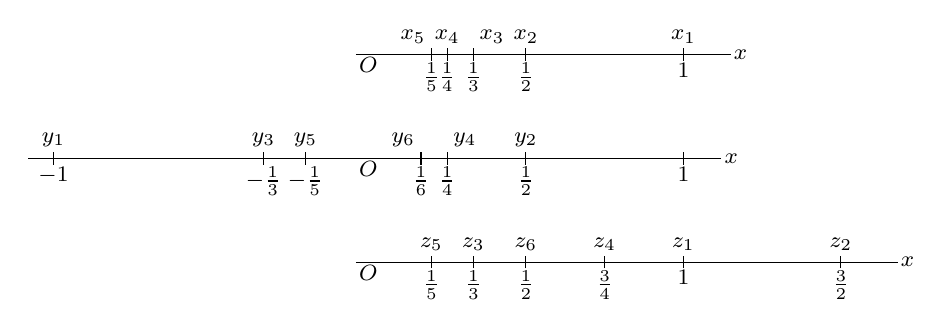
\begin{tikzpicture}[x=4cm,y=1.32cm,
      every node/.style={font=\footnotesize,inner sep=1pt}]
    % x_n
    \draw[line width=.45pt] (-.04,2) -- (1.15,2);
    \node[below] at (0,2) {\(O\)};
    \node[right] at (1.15,2) {\(x\)};
    \foreach \v in {.2,.25,.3333,.5,1}
      \draw[line width=.4pt] (\v,1.94) -- (\v,2.06);
    \node[above left=1pt] at (.2,2.05) {\(x_5\)};
    \node[above=1pt] at (.25,2.05) {\(x_4\)};
    \node[above right=1pt] at (.3333,2.05) {\(x_3\)};
    \node[above=1pt] at (.5,2.05) {\(x_2\)};
    \node[above=1pt] at (1,2.05) {\(x_1\)};
    \node[below] at (.2,1.95) {\(\frac15\)};
    \node[below] at (.25,1.95) {\(\frac14\)};
    \node[below] at (.3333,1.95) {\(\frac13\)};
    \node[below] at (.5,1.95) {\(\frac12\)};
    \node[below] at (1,1.95) {\(1\)};

    % y_n
    \draw[line width=.45pt] (-1.08,1) -- (1.12,1);
    \node[below] at (0,1) {\(O\)};
    \node[right] at (1.12,1) {\(x\)};
    \foreach \v in {-1,-.3333,-.2,.1667,.25,.5,1}
      \draw[line width=.4pt] (\v,.94) -- (\v,1.06);
    \node[above=1pt] at (-1,1.05) {\(y_1\)};
    \node[above=1pt] at (-.3333,1.05) {\(y_3\)};
    \node[above=1pt] at (-.2,1.05) {\(y_5\)};
    \node[above left=1pt] at (.1667,1.05) {\(y_6\)};
    \node[above right=1pt] at (.25,1.05) {\(y_4\)};
    \node[above=1pt] at (.5,1.05) {\(y_2\)};
    \node[below] at (-1,.95) {\(-1\)};
    \node[below] at (-.3333,.95) {\(-\frac13\)};
    \node[below] at (-.2,.95) {\(-\frac15\)};
    \node[below] at (.1667,.95) {\(\frac16\)};
    \node[below] at (.25,.95) {\(\frac14\)};
    \node[below] at (.5,.95) {\(\frac12\)};
    \node[below] at (1,.95) {\(1\)};

    % z_n
    \draw[line width=.45pt] (-.04,0) -- (1.68,0);
    \node[below] at (0,0) {\(O\)};
    \node[right] at (1.68,0) {\(x\)};
    \foreach \v in {.2,.3333,.5,.75,1,1.5}
      \draw[line width=.4pt] (\v,-.06) -- (\v,.06);
    \node[above=1pt] at (.2,.05) {\(z_5\)};
    \node[above=1pt] at (.3333,.05) {\(z_3\)};
    \node[above=1pt] at (.5,.05) {\(z_6\)};
    \node[above=1pt] at (.75,.05) {\(z_4\)};
    \node[above=1pt] at (1,.05) {\(z_1\)};
    \node[above=1pt] at (1.5,.05) {\(z_2\)};
    \node[below] at (.2,-.05) {\(\frac15\)};
    \node[below] at (.3333,-.05) {\(\frac13\)};
    \node[below] at (.5,-.05) {\(\frac12\)};
    \node[below] at (.75,-.05) {\(\frac34\)};
    \node[below] at (1,-.05) {\(1\)};
    \node[below] at (1.5,-.05) {\(\frac32\)};
  \end{tikzpicture}
  \caption{}
  \label{fig:3-1}
\end{figure}

\begin{mydef*}{}
我们称实数序列 \(\langle x_n\rangle\) \textbf{发散}，如果 \(\langle x_n\rangle\) 不收敛。
\end{mydef*}

由序列收敛的定义可知：
\[
\begin{aligned}
\langle x_n\rangle\text{ 发散}
&\iff(\forall\,a\in\R)\quad \lim_{n\to+\infty}x_n\neq a\\
&\iff(\forall\,a\in\R)(\exists\,\varepsilon_a>0)(\forall\,n\in\N)
   (\exists\,k_n\in\N,\ k_n\geqslant n)\\
&\hspace{7em}\Longrightarrow |x_{k_n}-a|\geqslant\varepsilon_a.
\end{aligned}
\]

\begin{sourceexample}{3}
证明：实数序列 \(\langle1+(-1)^n\rangle\) 发散。

事实上，\(\forall\,a\in\R\)，由
\[
\begin{aligned}
2=|2-a+a|
&\leqslant |2-a|+|a|\\
&=|1+(-1)^{2n}-a|+|1+(-1)^{2n-1}-a|
\end{aligned}
\]
推知
\[
|1+(-1)^{2n}-a|\geqslant1
\quad\text{或}\quad
|1+(-1)^{2n-1}-a|\geqslant1.
\]
因此
\[
\begin{aligned}
(\forall\,a\in\R)(\exists\,\varepsilon_a=1>0)(\forall\,n\in\N)
(\exists\,k_n\in\{2n,2n-1\},\ k_n\geqslant n)\\
\Longrightarrow |1+(-1)^{k_n}-a|\geqslant1.
\end{aligned}
\]
此即表明 \(\langle1+(-1)^n\rangle\) 发散。
\end{sourceexample}

直接从序列极限的定义可推出下述等价命题成立：
\[
\lim_{n\to+\infty}x_n=a
\iff
(\forall\,\varepsilon>0)(\exists\,N\in\N)
(\forall\,n\in\N,\ n\geqslant N)
\Longrightarrow |x_n-a|\leqslant M\varepsilon,
\]
这里 \(M\) 是与 \(n\) 无关的正数。

熟悉这一点，将给我们今后证明序列的极限带来方便。

现在我们介绍几个常用的方法。

\subsection{\texorpdfstring{用 \(\varepsilon\)-\(N\) 极限语言证明序列极限的方法}{用 ε-N 极限语言证明序列极限的方法}}

直接用 \(\varepsilon\)-\(N\) 极限语言证明 \(\lim_{n\to+\infty}x_n=a\) 没有万能的方法。总的原则是将差式
\(|x_n-a|\) 适当地放大成 \(|x_n-a|\leqslant A_n\) 的形式，使得表达式 \(A_n\) 的形式尽可能简洁，并由
\(A_n<\varepsilon\) 可方便地求出极限定义中所指的自然数 \(N\)。

下面就是几个一般的证明方法。

\subsubsection*{\texorpdfstring{1）直接变形求 \(A_n\)}{1）直接变形求 An}}

\begin{sourceexample}{4}
证明：
\[
\lim_{n\to+\infty}\sqrt[3]{n}\bigl(\sqrt[3]{n}-\sqrt[3]{n-1}\bigr)=0.
\]

\(\forall\,n\in\N\)，由于
\[
\begin{aligned}
&\left|\sqrt[3]{n}\bigl(\sqrt[3]{n}-\sqrt[3]{n-1}\bigr)-0\right|\\
&=\sqrt[3]{n}\bigl(\sqrt[3]{n}-\sqrt[3]{n-1}\bigr)\\
&=\frac{\sqrt[3]{n}\bigl(\sqrt[3]{n}-\sqrt[3]{n-1}\bigr)
\bigl(\sqrt[3]{n^2}+\sqrt[3]{n(n-1)}+\sqrt[3]{(n-1)^2}\bigr)}
{\sqrt[3]{n^2}+\sqrt[3]{n(n-1)}+\sqrt[3]{(n-1)^2}}\\
&=\frac{\sqrt[3]{n}}
{\sqrt[3]{n^2}+\sqrt[3]{n(n-1)}+\sqrt[3]{(n-1)^2}}
<\frac1{\sqrt[3]{n}}.
\end{aligned}
\]
故 \(\forall\,\varepsilon>0\)，由 \(\dfrac1{\sqrt[3]{n}}<\varepsilon\) 得到
\(n>\dfrac1{\varepsilon^3}\)。令
\[
N=\left[\frac1{\varepsilon^3}\right]+1,
\]
则
\[
\forall\,n\in\N,\quad n\geqslant N
\Longrightarrow
\left|\sqrt[3]{n}\bigl(\sqrt[3]{n}-\sqrt[3]{n-1}\bigr)-0\right|
<\frac1{\sqrt[3]{n}}<\varepsilon.
\]
因此
\[
\lim_{n\to+\infty}\sqrt[3]{n}\bigl(\sqrt[3]{n}-\sqrt[3]{n-1}\bigr)=0.
\]
\end{sourceexample}

\begin{sourceexample}{5}
证明：
\[
\lim_{n\to+\infty}
\left(\frac1{1\cdot2}+\frac1{2\cdot3}+\cdots+\frac1{n(n+1)}\right)=1.
\]

\(\forall\,n\in\N\)，由于
\[
\begin{aligned}
\frac1{1\cdot2}+\frac1{2\cdot3}+\cdots+\frac1{n(n+1)}
&=\left(1-\frac12\right)+\left(\frac12-\frac13\right)
 +\cdots+\left(\frac1n-\frac1{n+1}\right)\\
&=1-\frac1{n+1},
\end{aligned}
\]
故
\[
\left|
\frac1{1\cdot2}+\frac1{2\cdot3}+\cdots+\frac1{n(n+1)}-1
\right|
=\frac1{n+1}<\frac1n.
\]
\(\forall\,\varepsilon>0\)，由 \(\dfrac1n<\varepsilon\) 得到
\(n>\dfrac1\varepsilon\)。令
\[
N=\left[\frac1\varepsilon\right]+1,
\]
则
\[
\forall\,n\in\N,\quad n\geqslant N
\Longrightarrow
\left|
\frac1{1\cdot2}+\frac1{2\cdot3}+\cdots+\frac1{n(n+1)}-1
\right|<\varepsilon.
\]
因此
\[
\lim_{n\to+\infty}
\left(\frac1{1\cdot2}+\frac1{2\cdot3}+\cdots+\frac1{n(n+1)}\right)=1.
\]
\end{sourceexample}

\subsubsection*{\texorpdfstring{2）利用不等式求 \(A_n\)}{2）利用不等式求 An}}

\begin{sourceexample}{6}
证明：
\[
\lim_{n\to+\infty}
\frac{1\cdot3\cdots(2n-1)}{2\cdot4\cdots2n}=0.
\]

由不等式
\[
\frac{a+b}{2}\geqslant\sqrt{ab}\qquad(a\geqslant0,\ b\geqslant0)
\]
得到
\[
2=\frac{1+3}{2}\geqslant\sqrt{1\cdot3},\qquad
4=\frac{3+5}{2}\geqslant\sqrt{3\cdot5},\qquad\ldots,
\]
\[
2n=\frac{(2n-1)+(2n+1)}2\geqslant\sqrt{(2n-1)(2n+1)}.
\]
将这些不等式相乘得
\[
\begin{aligned}
2\cdot4\cdots2n
&\geqslant
\sqrt{1\cdot3}\sqrt{3\cdot5}\cdots\sqrt{(2n-1)(2n+1)}\\
&=1\cdot3\cdots(2n-1)\sqrt{2n+1}.
\end{aligned}
\]
由此得到
\[
\frac{1\cdot3\cdots(2n-1)}{2\cdot4\cdots2n}
<\frac1{\sqrt{2n+1}}<\frac1{\sqrt n}.
\]
\(\forall\,\varepsilon>0\)，由 \(\dfrac1{\sqrt n}<\varepsilon\) 得到
\(n>\dfrac1{\varepsilon^2}\)。令
\[
N=\left[\frac1{\varepsilon^2}\right]+1,
\]
则
\[
\forall\,n\in\N,\quad n\geqslant N
\Longrightarrow
\left|
\frac{1\cdot3\cdots(2n-1)}{2\cdot4\cdots2n}-0
\right|
<\frac1{\sqrt n}<\varepsilon.
\]
因此
\[
\lim_{n\to+\infty}
\frac{1\cdot3\cdots(2n-1)}{2\cdot4\cdots2n}=0.
\]
\end{sourceexample}

\begin{sourceexample}{7}
证明：
\[
\lim_{n\to+\infty}\frac1{\sqrt[n]{n!}}=0.
\]

由于 \(\forall\,n\in\N\)，
\[
\begin{aligned}
(n!)^2=n!\cdot n!
&=1\cdot n\cdot2\cdot(n-1)\cdots k(n-k+1)\cdots n\cdot1,
\end{aligned}
\]
并且
\[
\forall\,k,n\in\N,\quad k\leqslant n
\Longrightarrow k(n-k+1)\geqslant n,
\]
故
\[
(n!)^2\geqslant n\cdot n\cdots n=n^n.
\]
由此推得
\[
\sqrt[n]{n!}\geqslant\sqrt n,
\qquad\text{或}\qquad
\frac1{\sqrt[n]{n!}}\leqslant\frac1{\sqrt n}.
\]
\(\forall\,\varepsilon>0\)，由 \(\dfrac1{\sqrt n}<\varepsilon\) 得到
\(n>\dfrac1{\varepsilon^2}\)。令
\[
N=\left[\frac1{\varepsilon^2}\right]+1,
\]
则
\[
\forall\,n\in\N,\quad n\geqslant N
\Longrightarrow
\left|\frac1{\sqrt[n]{n!}}-0\right|
\leqslant\frac1{\sqrt n}<\varepsilon.
\]
因此
\[
\lim_{n\to+\infty}\frac1{\sqrt[n]{n!}}=0.
\]
\end{sourceexample}

\subsubsection*{\texorpdfstring{3）利用二项式展开求 \(A_n\)}{3）利用二项式展开求 An}}

\begin{sourceexample}{8}
证明：\(\forall\,q\in\R,\ |q|<1\)，
\[
\lim_{n\to+\infty}q^n=0.
\]

若 \(q=0\)，则结论显然成立。

若 \(q\neq0\)，则由于 \(|q|<1\)，有 \(\dfrac1{|q|}>1\)。令
\[
a=\frac1{|q|}-1,
\]
则 \(a>0\)，并且
\[
|q|=\frac1{1+a},\qquad |q|^n=\frac1{(1+a)^n}.
\]
由二项式展开公式得到
\[
(1+a)^n=1+na+\frac{n(n-1)}2a^2+\cdots+a^n>na,
\]
所以
\[
|q^n-0|=|q|^n=\frac1{(1+a)^n}<\frac1{na}.
\]
\(\forall\,\varepsilon>0\)，由 \(\dfrac1{na}<\varepsilon\) 得到
\(n>\dfrac1{a\varepsilon}\)。令
\[
N=\left[\frac1{a\varepsilon}\right]+1,
\]
则
\[
\forall\,n\in\N,\quad n\geqslant N
\Longrightarrow |q^n-0|<\frac1{na}<\varepsilon.
\]
因此
\[
\lim_{n\to+\infty}q^n=0.
\]
\end{sourceexample}

\begin{sourceexample}{9}
证明：\(\forall\,q\in\R,\ |q|<1\)，
\[
\lim_{n\to+\infty}nq^n=0.
\]

若 \(q=0\)，则结论显然成立。

若 \(q\neq0\)，则像上一题一样，令
\[
a=\frac1{|q|}-1>0.
\]
于是
\[
n|q|^n=\frac{n}{(1+a)^n}\qquad(n\in\N).
\]
由于
\[
(1+a)^n
=1+na+\frac{n(n-1)}2a^2+\cdots+a^n
>\frac{n(n-1)}2a^2,
\]
故
\[
|nq^n-0|
=n|q|^n
<\frac{n}{\frac{n(n-1)}2a^2}
=\frac2{(n-1)a^2}
\qquad(n\geqslant2).
\]
\(\forall\,\varepsilon>0\)，由
\(\dfrac2{(n-1)a^2}<\varepsilon\) 得到
\(n>1+\dfrac2{a^2\varepsilon}\)。令
\[
N=1+\left[1+\frac2{a^2\varepsilon}\right],
\]
则
\[
\forall\,n\in\N,\quad n\geqslant N
\Longrightarrow
|nq^n-0|<\frac2{(n-1)a^2}<\varepsilon.
\]
因此
\[
\lim_{n\to+\infty}nq^n=0.
\]
\end{sourceexample}

\subsubsection*{\texorpdfstring{4）分析法求 \(A_n\)}{4）分析法求 An}}

\begin{sourceexample}{10}
证明：
\[
\lim_{n\to+\infty}\frac{a^n}{n!}=0
\qquad(a\neq0).
\]

首先，\(\forall\,n,m\in\N\) 且 \(m\leqslant n\)，我们有
\[
\begin{aligned}
\left|\frac{a^n}{n!}-0\right|
&=\frac{|a|^n}{n!}\\
&=\left(\frac{|a|}{1}\frac{|a|}{2}\cdots\frac{|a|}{m-1}\right)
  \left(\frac{|a|}{m}\cdots\frac{|a|}{n-1}\right)\frac{|a|}{n}.
\end{aligned}
\]
若取 \(m\geqslant|a|\)，则
\[
\left|\frac{a^n}{n!}-0\right|
<\frac{|a|^{m-1}}{(m-1)!}\cdot1\cdots1\cdot\frac{|a|}{n}
=\frac Mn,
\]
这里
\[
M=\frac{|a|^m}{(m-1)!}>0.
\]
\(\forall\,\varepsilon>0\)，由 \(\dfrac Mn<\varepsilon\) 得到
\(n>\dfrac M\varepsilon\)。令
\[
N=\max\left(m,\left[\frac M\varepsilon\right]+1\right),
\]
则
\[
\forall\,n\in\N,\quad n\geqslant N
\Longrightarrow
\left|\frac{a^n}{n!}-0\right|<\frac Mn<\varepsilon.
\]
因此
\[
\lim_{n\to+\infty}\frac{a^n}{n!}=0.
\]
\end{sourceexample}

\begin{sourceexample}{11}
证明：若
\[
\lim_{n\to+\infty}x_n=a,
\]
则
\[
\lim_{n\to+\infty}\frac{x_1+x_2+\cdots+x_n}{n}=a.
\]

由于 \(\lim_{n\to+\infty}x_n=a\)，故由定义
\[
(\forall\,\varepsilon>0)(\exists\,N_1\in\N)
(\forall\,n\in\N,\ n\geqslant N_1)
\Longrightarrow |x_n-a|<\frac\varepsilon2.
\]
因此 \(\forall\,n\geqslant N_1\)，
\[
\begin{aligned}
\left|\frac{x_1+x_2+\cdots+x_n}{n}-a\right|
&=\left|\frac{x_1+x_2+\cdots+x_n-na}{n}\right|\\
&\leqslant
\left|\frac{(x_1-a)+\cdots+(x_{N_1}-a)}{n}\right|\\
&\quad+
\left|\frac{(x_{N_1+1}-a)+\cdots+(x_n-a)}{n}\right|\\
&<\frac{|(x_1-a)+\cdots+(x_{N_1}-a)|}{n}
+\frac{n-N_1}{n}\frac\varepsilon2\\
&<\frac Mn+\frac\varepsilon2,
\end{aligned}
\]
这里
\[
M=|(x_1-a)+\cdots+(x_{N_1}-a)|\geqslant0.
\]
由 \(\dfrac Mn<\dfrac\varepsilon2\) 得到
\(n>\dfrac{2M}{\varepsilon}\)。令
\[
N=\max\left(N_1,\left[\frac{2M}{\varepsilon}\right]+1\right),
\]
则
\[
\begin{aligned}
\forall\,n\in\N,\quad n\geqslant N
&\Longrightarrow
\left|\frac{x_1+x_2+\cdots+x_n}{n}-a\right|
<\frac Mn+\frac\varepsilon2\\
&<\frac\varepsilon2+\frac\varepsilon2=\varepsilon.
\end{aligned}
\]
因此
\[
\lim_{n\to+\infty}\frac{x_1+x_2+\cdots+x_n}{n}=a.
\]
\end{sourceexample}

\subsection*{习 题}
\begin{exercise}
  \item 证明下列结论等价：
  \begin{enumerate}[label=\arabic*)]
    \item \(\displaystyle\lim_{n\to+\infty}x_n=a\)；
    \item \((\forall\,\varepsilon>0)(\exists\,N\in\N)
      (\forall\,n\in\N,\ n\geqslant N)
      \Longrightarrow |x_n-a|<M\varepsilon\)，其中 \(M\) 为常数；
    \item \((\forall\,k\in\N)(\exists\,N\in\N)
      (\forall\,n\in\N,\ n\geqslant N)
      \Longrightarrow |x_n-a|<\dfrac1k\)。
  \end{enumerate}
\end{exercise}

\begin{exercise}
  \item 证明：实数序列 \(\langle(-1)^n\rangle\) 发散。
\end{exercise}

\begin{exercise}
  \item 证明：\(\forall\,a\in\R\)，
  \[
  \lim_{n\to+\infty}\frac{[na]}n=a.
  \]
\end{exercise}

\begin{exercise}
  \item 证明：若 \(\displaystyle\lim_{n\to+\infty}x_n=a\)，则
  \[
  \lim_{n\to+\infty}|x_n|=|a|.
  \]
  举例说明逆命题不成立。
\end{exercise}

\begin{exercise}
  \item 证明：
  \[
  \lim_{n\to+\infty}x_n=a
  \]
  当且仅当
  \[
  \lim_{n\to+\infty}x_{2n}
  =\lim_{n\to+\infty}x_{2n+1}=a.
  \]
\end{exercise}

\begin{exercise}
  \item 用 \(\varepsilon\)-\(N\) 语言证明下列各极限：
  \begin{enumerate}[label=\arabic*)]
    \item \(\displaystyle\lim_{n\to+\infty}\frac{n!}{n^n}=0\)；
    \item \(\displaystyle\lim_{n\to+\infty}\sqrt[n]{a}=1\quad(a>0)\)；
    \item \(\displaystyle\lim_{n\to+\infty}\frac{n^k}{a^n}=0
      \quad(a>1,\ k\in\N)\)；
    \item \(\displaystyle\lim_{n\to+\infty}\sqrt[n]{n^k}=1
      \quad(k\in\N)\)；
    \item \(\displaystyle\lim_{n\to+\infty}\left(\sqrt[k]{n}\right)^{1/n}=1
      \quad(k\in\N)\)；
    \item \(\displaystyle\lim_{n\to+\infty}
      \left(\frac1{n^2}+\frac1{(n+1)^2}+\cdots+\frac1{(2n)^2}\right)=0\)；
    \item \(\displaystyle\lim_{n\to+\infty}
      \left(\frac1{n^2}+\frac2{n^2}+\cdots+\frac n{n^2}\right)=\frac12\)；
    \item \(\displaystyle\lim_{n\to+\infty}
      \left(\frac12+\frac2{2^2}+\cdots+\frac n{2^n}\right)=2\)；
    \item \(\displaystyle\lim_{n\to+\infty}
      \frac32\cdot\frac54\cdots
      \frac{2^{2^n}+1}{2^{2^n}}=2\)；
    \item \(\displaystyle\lim_{n\to+\infty}
      \left(\frac12+\frac3{2^2}+\cdots+\frac{2n-1}{2^n}\right)=3\)。
  \end{enumerate}
\end{exercise}

\begin{exercise}
  \item 设 \(\langle x_n\rangle\) 是任一实数序列，使得
  \[
  \lim_{n\to+\infty}(x_{n+1}-x_n)=0.
  \]
  证明：
  \[
  \lim_{n\to+\infty}\frac{x_n}{n}=0.
  \]
\end{exercise}

\begin{exercise}
  \item 设 \(a_0,a_1,\ldots,a_k\in\R\)，使得
  \[
  a_0+a_1+\cdots+a_k=0.
  \]
  证明：
  \[
  \lim_{n\to+\infty}
  \left(a_0\sqrt n+a_1\sqrt{n+1}+\cdots+a_k\sqrt{n+k}\right)=0.
  \]
\end{exercise}

\begin{exercise}
  \item 设 \(\langle x_n\rangle\) 是任一实数序列，并且
  \[
  \lim_{n\to+\infty}x_n=a.
  \]
  \begin{enumerate}[label=\arabic*)]
    \item 证明：
    \[
    \lim_{n\to+\infty}\frac{x_1+2x_2+\cdots+nx_n}{n^2}=\frac a2.
    \]
    \item 利用 1）的结论计算下列各极限值（\(0<a<1\)）：
    \[
    \lim_{n\to+\infty}
    \frac1{n^2}\left(a+2^2a^2+\cdots+n^2a^n\right),
    \]
    \[
    \lim_{n\to+\infty}
    \frac1{n^2}\left(1+\sqrt{2^3}+\sqrt[3]{3^4}
    +\cdots+\sqrt[n]{n^{n+1}}\right).
    \]
  \end{enumerate}
\end{exercise}

\begin{exercise}
  \item 分别利用极限定义及反证法证明序列 \(\langle\sin n\rangle\) 发散。
\end{exercise}

\begin{exercise}
  \item 设 \(\langle a_n\rangle\) 是一实数序列，令
  \[
  b_n=a_{n-1}+2a_n\qquad(n\in\N,\ n\geqslant2).
  \]
  证明：若序列 \(\langle b_n\rangle\) 收敛，则序列 \(\langle a_n\rangle\) 也收敛，并且
  \[
  \lim_{n\to+\infty}b_n=3\lim_{n\to+\infty}a_n.
  \]
\end{exercise}

\begin{exercise}
  \item 设实数序列 \(\langle a_n\rangle\) 满足条件
  \[
  \lim_{n\to+\infty}(a_n-a_{n-2})=0.
  \]
  证明：
  \[
  \lim_{n\to+\infty}\frac1n(a_n-a_{n-1})=0.
  \]
\end{exercise}

\begin{exercise}
  \item 设 \(X\subset\R\) 是任一非空集合。证明：\(X\) 是闭集的充分必要条件是
  \[
  \forall\,x_n\in X\ (n\in\N),\quad
  x_n\to x\ (n\to+\infty)
  \Longrightarrow x\in X.
  \]
\end{exercise}

\section{收敛序列的性质}

\subsection{收敛序列的一般性质}

\begin{myproperty}{}{limit-uniqueness}
如果实数序列 \(\langle x_n\rangle\) 收敛，则此序列的极限是唯一的。
\end{myproperty}

\begin{proof}
设 \(\lim_{n\to+\infty}x_n=a\)，\(\lim_{n\to+\infty}x_n=b\)，并且 \(a\ne b\)。于是由 \(\R\) 的 Hausdorff 分离性，存在 \(\delta>0\) 使得
\[
B(a,\delta)\cap B(b,\delta)=\varnothing.
\]
另一方面，对 \(\delta>0\)，存在 \(N_1,N_2\in\N\)，使得
\[
\forall n\in\N,\quad n\geqslant N_1\Longrightarrow x_n\in B(a,\delta),
\]
\[
\forall n\in\N,\quad n\geqslant N_2\Longrightarrow x_n\in B(b,\delta).
\]
令 \(N=\max(N_1,N_2)\)，则
\[
\forall n\in\N,\quad n\geqslant N
\Longrightarrow x_n\in B(a,\delta)\cap B(b,\delta).
\]
这与 \(B(a,\delta)\cap B(b,\delta)=\varnothing\) 相矛盾。因此 \(a=b\)。
\end{proof}

\begin{myproperty}{}{finite-modification-preserves-limit}
如果 \(\lim_{n\to+\infty}x_n=a\)，则任意改变 \(\langle x_n\rangle\) 的有限多项后所得新的实数序列 \(\langle y_n\rangle\) 也有
\[
\lim_{n\to+\infty}y_n=a.
\]
\end{myproperty}

证明留给读者。

\begin{myproperty}{}{convergent-sequence-bounded}
如果实数序列 \(\langle x_n\rangle\) 收敛，则 \(\langle x_n\rangle\) 是有界的，即
\[
(\exists M>0)(\forall n\in\N)\Longrightarrow |x_n|\leqslant M.
\]
\end{myproperty}

\begin{proof}
设 \(\lim_{n\to+\infty}x_n=a\)。于是对 \(\varepsilon=1\)，存在 \(N\in\N\)，使得
\[
\forall n\in\N,\quad n\geqslant N\Longrightarrow |x_n-a|<1
\Longrightarrow |x_n|\leqslant |x_n-a|+|a|<1+|a|.
\]
令
\[
M=\max(|x_1|,|x_2|,\dots,|x_{N-1}|,1+|a|),
\]
则 \(\forall n\in\N\)，\(|x_n|\leqslant M\)。
\end{proof}

\begin{myproperty}{}{subsequence-preserves-limit}
如果 \(\lim_{n\to+\infty}x_n=a\)，则对任一映射 \(k\colon\N\to\N\)，若
\[
k(n)<k(n+1)\quad(\forall n\in\N),
\]
也有 \(\lim_{n\to+\infty}x_{k(n)}=a\)。
\end{myproperty}

序列 \(\langle x_{k(n)}\rangle\) 称为 \(\langle x_n\rangle\) 的子序列，\(\langle x_{k(n)}\rangle\) 也常记为 \(\langle x_{k_n}\rangle\)。

\begin{proof}
因为 \(\lim_{n\to+\infty}x_n=a\)，所以由定义
\[
(\forall\varepsilon>0)(\exists N\in\N)(\forall n\in\N, n\geqslant N)
\Longrightarrow |x_n-a|<\varepsilon.
\]
现设 \(k\colon\N\to\N\) 是任一严格单调上升映射。由归纳法可证
\[
\forall n\in\N,\quad k(n)\geqslant n.
\]
由此推得
\[
\forall n\in\N,\quad n\geqslant N\Longrightarrow k(n)\geqslant N
\Longrightarrow |x_{k(n)}-a|<\varepsilon.
\]
因此 \(\lim_{n\to+\infty}x_{k(n)}=a\)。
\end{proof}

\begin{sourceexample}{1}
利用\rprop{property:subsequence-preserves-limit}证明实数序列 \(\langle1+(-1)^n\rangle\) 发散。

定义严格单调上升映射 \(k,l\colon\N\to\N\) 如下：
\[
k(n)=2n,\quad l(n)=2n-1\quad(\forall n\in\N).
\]
那么
\[
1+(-1)^{k(n)}=2,\quad 1+(-1)^{l(n)}=0\quad(\forall n\in\N).
\]
因此
\[
\lim_{n\to+\infty}[1+(-1)^{k(n)}]=2,\quad
\lim_{n\to+\infty}[1+(-1)^{l(n)}]=0.
\]
由\rprop{property:subsequence-preserves-limit}知，序列 \(\langle1+(-1)^n\rangle\) 发散。
\end{sourceexample}

\begin{sourceexample}{2}
设 \(p\in\N\)，\(\langle x_n\rangle\) 是一实数序列，满足
\[
x_n=x_{n+p}\quad(\forall n\in\N).
\]
证明：若 \(\lim_{n\to+\infty}x_n=a\)，则 \(x_n=a\ (\forall n\in\N)\)。

为此，考虑 \(p\) 个严格单调上升映射 \(k^{(i)}\colon\N\to\N\ (i=1,2,\dots,p)\)，它们定义为
\[
k^{(i)}(n)=i+(n-1)p,\quad \forall n\in\N\quad(i=1,2,\dots,p).
\]
由于 \(\lim_{n\to+\infty}x_n=a\)，故
\[
\forall i=1,2,\dots,p,\quad
\lim_{n\to+\infty}x_{k^{(i)}(n)}=a.
\]
另一方面，由假设 \(x_n=x_{n+p}\ (\forall n\in\N)\)，我们有
\[
x_{k^{(i)}(n)}=x_{k^{(i)}(n+1)},\quad
\forall n\in\N\quad(i=1,2,\dots,p).
\]
因此 \(x_{k^{(i)}(n)}\equiv a\ (\forall n\in\N)\ (i=1,2,\dots,p)\)，从而 \(x_n\equiv a\ (\forall n\in\N)\)。
\end{sourceexample}

\subsection{收敛序列极限的运算性质}

\begin{myproperty}{}{limit-arithmetic}
设 \(\lim_{n\to+\infty}x_n=a\)，\(\lim_{n\to+\infty}y_n=b\)。则实数序列
\[
\langle x_n+y_n\rangle,\quad \langle x_ny_n\rangle,\quad
\left\langle\frac{x_n}{y_n}\right\rangle\quad(b\ne0)
\]
也收敛，并且
\begin{enumerate}[label=\arabic*)]
  \item \(\displaystyle\lim_{n\to+\infty}(x_n+y_n)=a+b\)；
  \item \(\displaystyle\lim_{n\to+\infty}x_ny_n=ab\)；
  \item \(\displaystyle\lim_{n\to+\infty}\frac{x_n}{y_n}=\frac ab\quad(b\ne0)\)。
\end{enumerate}
\end{myproperty}

\begin{proof}

因为 \(\lim_{n\to+\infty}x_n=a\)，\(\lim_{n\to+\infty}y_n=b\)，所以
\[
(\forall\varepsilon>0)(\exists N\in\N)(\forall n\in\N, n\geqslant N)
\Longrightarrow
\begin{cases}
|x_n-a|<\varepsilon,\\
|y_n-b|<\varepsilon,\quad |y_n|<|b|+\varepsilon.
\end{cases}
\]

由此推得

\[\forall n \in \mathbb{N}, n \geqslant N\]

\[\Longrightarrow
\begin{cases}
|(x_n+y_n)-(a+b)|\leqslant|x_n-a|+|y_n-b|<2\varepsilon,\\
|x_ny_n-ab|\leqslant|y_n||x_n-a|+|a||y_n-b|
<( |a|+|b|+\varepsilon)\varepsilon.
\end{cases}
\]

因此\(\langle x_n + y_n \rangle\) 及\(\langle x_n y_n \rangle\) 收敛,并且\(\lim_{n \to +\infty} (x_n + y_n) = a + b\) ,\(\lim_{n \to +\infty} x_n y_n = ab\) .

若 \(b\ne0\)，则不妨设 \(0<\varepsilon<|b|/2\)。由 \(|y_n-b|<\varepsilon\) 推得
\[
|y_n|>|b|-\varepsilon\geqslant\frac{|b|}{2}\quad(\forall n\in\N,\ n\geqslant N).
\]
因此
\[
\begin{aligned}
\forall n\in\N,\quad n\geqslant N\Longrightarrow
\left|\frac{x_n}{y_n}-\frac ab\right|
&=\frac{|x_nb-y_na|}{|b|\,|y_n|}\\
&\leqslant\frac{2}{|b|^2}\bigl(|x_nb-ab|+|y_na-ab|\bigr)\\
&\leqslant\frac{2(|a|+|b|)}{|b|^2}\varepsilon.
\end{aligned}
\]

从而 \(\left\langle x_n/y_n\right\rangle\) 收敛，并且
\(\lim_{n\to+\infty}x_n/y_n=a/b\)。

\end{proof}

\begin{mycor*}{}
若 \(\lim_{n\to+\infty}x_n=a\)，\(b\in\R\)，则
\[
\lim_{n\to+\infty}(x_n+b)=a+b,\qquad
\lim_{n\to+\infty}x_nb=ab,
\]
\[
\lim_{n\to+\infty}\frac1{x_n}=\frac1a\quad(a\ne0).
\]
\end{mycor*}

\begin{sourceexample}{3}
由于 \(\forall p\in\N\)，\(\lim_{n\to+\infty}1/n^p=0\)，及
\[
\begin{aligned}
&\frac{a_k n^k+a_{k-1}n^{k-1}+\cdots+a_1n+a_0}
       {b_m n^m+b_{m-1}n^{m-1}+\cdots+b_1n+b_0}\\
&\qquad=
\frac{a_k+a_{k-1}/n+\cdots+a_1/n^{k-1}+a_0/n^k}
     {b_m+b_{m-1}/n+\cdots+b_1/n^{m-1}+b_0/n^m}\,n^{k-m}.
\end{aligned}
\]

因此

\[\lim_{n \to +\infty} \frac{a_k n^k + a_{k-1} n^{k-1} + \cdots + a_1 n + a_0}{b_m n^m + b_{m-1} n^{m-1} + \cdots + b_1 n + b_0}\]

\[= \begin{cases} \dfrac{a_k}{b_m}, & k=m, \\ 0, & k<m. \end{cases}\]

从而

\[\lim_{n\to+\infty} \frac{3n^3-1}{2n^3+n^2+1} = \frac{3}{2},\]

\[\lim_{n\to+\infty} \frac{4n^2+n+1}{5n^3+2n-1} = 0.\]
\end{sourceexample}

\subsection{收敛序列的不等式性质}

\begin{myproperty}{}{limit-eventual-order}
如果 \(\lim_{n\to+\infty}x_n=a\)，并且 \(a>r\)（\(a<r\)），则
\[
(\exists N\in\N)(\forall n\in\N, n\geqslant N)
\Longrightarrow x_n>r\quad(x_n<r).
\]
\end{myproperty}

\begin{proof}
设 \(a>r\)。对于 \(\varepsilon=a-r>0\)，存在 \(N\in\N\)，使得
\[
\forall n\in\N,\quad n\geqslant N\Longrightarrow |x_n-a|<a-r
\Longrightarrow x_n>a-(a-r)=r.
\]
类似可证 \(a<r\) 的情形。
\end{proof}

\begin{myproperty}{}{limit-strict-comparison}
如果 \(\lim_{n\to+\infty}x_n=a\)，\(\lim_{n\to+\infty}y_n=b\)，并且 \(a>b\)（\(a<b\)），则
\[
(\exists N\in\N)(\forall n\in\N, n\geqslant N)
\Longrightarrow x_n>y_n\quad(x_n<y_n).
\]
\end{myproperty}

\begin{proof}
设 \(a>b\)。于是存在 \(r\in\R\)，使得 \(a>r>b\)。由
\[
\lim_{n\to+\infty}x_n=a>r>b=\lim_{n\to+\infty}y_n
\]
及\rprop{property:limit-eventual-order}知，存在 \(N_1,N_2\in\N\)，使得
\[
\forall n\in\N,\quad n\geqslant N_1\Longrightarrow x_n>r,
\]
\[
\forall n\in\N,\quad n\geqslant N_2\Longrightarrow y_n<r.
\]
令 \(N=\max(N_1,N_2)\)，则
\[
\forall n\in\N,\quad n\geqslant N\Longrightarrow x_n>y_n.
\]
对 \(a<b\)，可类似证明。
\end{proof}

\begin{myproperty}{}{limit-preserves-order}
设 \(\lim_{n\to+\infty}x_n=a\)，\(\lim_{n\to+\infty}y_n=b\)，则
\[
\forall n\geqslant N,\quad x_n\geqslant y_n\quad(x_n\leqslant y_n)
\Longrightarrow a\geqslant b\ (a\leqslant b).
\]
\end{myproperty}

\begin{proof}
用反证法，由\rprop{property:limit-strict-comparison}立即推出。
\end{proof}

\begin{mycor*}{}
如果 \(\lim_{n\to+\infty}x_n=a\)，并且 \(\forall n\geqslant N\)，
\(x_n\geqslant r\ (x_n\leqslant r)\)，则 \(a\geqslant r\ (a\leqslant r)\)。
\end{mycor*}

注意，即使在\rprop{property:limit-preserves-order}中将不等号“\(\geqslant\)（\(\leqslant\)）”换成严格不等号“\(>\)（\(<\)）”，也不一定有 \(a>b\ (a<b)\)。例如，取
\[
x_n=\frac1n,\qquad y_n=-\frac1n\quad(n\in\N).
\]
显然有 \(x_n>y_n\ (\forall n\in\N)\)，但是
\(\lim_{n\to+\infty}x_n=\lim_{n\to+\infty}y_n=0\)。

\begin{myproperty}{}{squeeze-theorem}
设实数序列 \(\langle x_n\rangle\)、\(\langle y_n\rangle\)、\(\langle z_n\rangle\) 满足下述条件：
\begin{enumerate}[label=\arabic*)]
  \item \(x_n\leqslant z_n\leqslant y_n\quad(\forall n\in\N, n\geqslant N)\)；
  \item \(\displaystyle\lim_{n\to+\infty}x_n=\lim_{n\to+\infty}y_n=a\)，
\end{enumerate}
则 \(\lim_{n\to+\infty}z_n=a\)。
\end{myproperty}

\begin{proof}
由已知条件，对任意 \(\varepsilon>0\)，存在 \(N_0\in\N\)，\(N_0\geqslant N\)，使得
\[
\forall n\in\N,\quad n\geqslant N_0
\Longrightarrow |x_n-a|<\varepsilon,\quad |y_n-a|<\varepsilon.
\]
由此推得
\[
a-\varepsilon<x_n\leqslant z_n\leqslant y_n<a+\varepsilon
\Longrightarrow |z_n-a|<\varepsilon.
\]
因此 \(\lim_{n\to+\infty}z_n=a\)。
\end{proof}

\rprop{property:squeeze-theorem}常称为序列极限的两边夹法则。

\begin{sourceexample}{4}
设
\[
x_n=\frac{n}{\sqrt{n^2+n}},\qquad
y_n=\frac{n}{\sqrt{n^2+1}},
\]
\[
z_n=\frac1{\sqrt{n^2+1}}+\frac1{\sqrt{n^2+2}}+\cdots+\frac1{\sqrt{n^2+n}}
\quad(n\in\N).
\]
证明：
\[
\lim_{n\to+\infty}x_n=\lim_{n\to+\infty}y_n=\lim_{n\to+\infty}z_n=1.
\]
首先由不等式
\[
1<\sqrt{1+\frac1{n^2}}\leqslant\sqrt{1+\frac1n}<1+\frac1n
\quad(\forall n\in\N)
\]
及\rprop{property:squeeze-theorem}推得
\[
\lim_{n\to+\infty}\sqrt{1+\frac1n}
=\lim_{n\to+\infty}\sqrt{1+\frac1{n^2}}=1.
\]
因此
\[
\lim_{n\to+\infty}x_n=1,\qquad \lim_{n\to+\infty}y_n=1.
\]
另一方面，由于
\[
x_n=\underbrace{\frac1{\sqrt{n^2+n}}+\cdots+\frac1{\sqrt{n^2+n}}}_{n\text{ 项}}
<z_n<\frac{n}{\sqrt{n^2+1}}=y_n,
\]
故 \(x_n\leqslant z_n\leqslant y_n\ (\forall n\in\N)\)。从而由\rprop{property:squeeze-theorem}得到
\[
\lim_{n\to+\infty}z_n=1.
\]
\end{sourceexample}

\begin{sourceexample}{5}
设 \(\langle x_n\rangle\) 是任一实数序列，并且
\(x_n\leqslant x_{n+1}\ (\forall n\in\N)\)。证明：若
\[
\lim_{n\to+\infty}\frac{x_1+x_2+\cdots+x_n}{n}=a,
\]
则 \(\lim_{n\to+\infty}x_n=a\)。

令 \(y_n=(x_1+x_2+\cdots+x_n)/n\)。首先有
\[
y_n\leqslant x_n\quad(\forall n\in\N).
\]
现在任意固定 \(n\in\N\)。\(\forall m\geqslant n\)，
\[
y_m=\frac{x_1+\cdots+x_n}{m}+\frac{x_{n+1}+\cdots+x_m}{m}
\geqslant\frac{x_1+\cdots+x_n}{m}+\left(\frac{m-n}{m}\right)x_n.
\]
两边令 \(m\to+\infty\)，由\rprop{property:limit-preserves-order}得到
\[
a=\lim_{m\to+\infty}y_m
\geqslant\lim_{m\to+\infty}\frac{x_1+\cdots+x_n}{m}
+\lim_{m\to+\infty}\left(\frac{m-n}{m}\right)x_n=x_n.
\]
由此得到
\[
y_n\leqslant x_n\leqslant a\quad(\forall n\in\N).
\]
由于 \(\lim_{n\to+\infty}y_n=a\)，故由\rprop{property:squeeze-theorem}立即推得
\(\lim_{n\to+\infty}x_n=a\)。
\end{sourceexample}

\subsection*{习 题}

\begin{exercise}
  \item 设 \(\langle x_n\rangle\) 是任一实数序列，满足
  \(x_n\leqslant x_{n+1}\ (\forall n\in\N)\) 或
  \(x_n\geqslant x_{n+1}\ (\forall n\in\N)\)。如果存在
  \(\langle x_n\rangle\) 的一个子序列 \(\langle x_{k(n)}\rangle\)，使得
  \(\lim_{n\to+\infty}x_{k(n)}=a\)，则
  \(\lim_{n\to+\infty}x_n=a\)。
\end{exercise}

\begin{exercise}
  \item 计算下列各极限：
  \begin{enumerate}[label=\arabic*)]
    \item \(\displaystyle\lim_{n\to+\infty}\frac{\sqrt n}{\sqrt{n+\sqrt{n+\sqrt n}}}\)；
    \item \(\displaystyle\lim_{n\to+\infty}(\sqrt{n+1}-\sqrt n)\sqrt n\)；
    \item \(\displaystyle\lim_{n\to+\infty}\frac{\sqrt[3]{n^2+1}}{n+2}\)；
    \item \(\displaystyle\lim_{n\to+\infty}\left(\frac1{1\cdot3}+\frac1{2\cdot4}+\cdots+\frac1{n(n+2)}\right)\)；
    \item \(\displaystyle\lim_{n\to+\infty}\sum_{k=1}^{n}\frac1{(k+p)(k+p+q)}\quad(p,q\in\N)\)；
    \item \(\displaystyle\lim_{n\to+\infty}\sum_{k=1}^{n}\frac1{k(k+1)(k+2)}\)。
  \end{enumerate}
\end{exercise}

\begin{exercise}
  \item 设 \(\lim_{n\to+\infty}a_n=a\)，\(\lim_{n\to+\infty}b_n=b\)。证明：
  \begin{enumerate}[label=\arabic*)]
    \item \(\displaystyle\lim_{n\to+\infty}\max(a_n,b_n)=\max(a,b)\)；
    \item \(\displaystyle\lim_{n\to+\infty}\min(a_n,b_n)=\min(a,b)\)。
  \end{enumerate}
\end{exercise}

\begin{exercise}
  \item 设 \(\langle a_n\rangle\) 是任一严格正的实数序列，并且
  \(\lim_{n\to+\infty}a_n=0\)。证明：
  \begin{enumerate}[label=\arabic*)]
    \item 集合 \(\{n\in\N\mid \forall k\geqslant n, a_k\leqslant a_n\}\) 是无限集；
    \item 集合 \(\{n\in\N\mid \forall k\leqslant n, a_n\leqslant a_k\}\) 是无限集。
  \end{enumerate}
\end{exercise}

\begin{exercise}
  \item 设 \(\langle a_n\rangle\)、\(\langle b_n\rangle\) 是任意两个实数序列，并且
  \(\lim_{n\to+\infty}a_n=a\)，\(\lim_{n\to+\infty}b_n=b\)。定义序列 \(\langle c_n\rangle\) 如下：
  \[
  c_n=\frac1n(a_1b_n+a_2b_{n-1}+\cdots+a_nb_1)\quad(n\in\N).
  \]
  \begin{enumerate}[label=\arabic*)]
    \item 证明：存在常数 \(M>0\) 使得
    \[
    |c_n-ab|\leqslant\frac Mn\sum_{i=1}^{n}(|a_i-a|+|b_i-b|).
    \]
    \item 证明：\(\displaystyle\lim_{n\to+\infty}c_n=ab\)。
  \end{enumerate}
\end{exercise}

\begin{exercise}
  \item 设 \(\langle a_n\rangle\)、\(\langle b_n\rangle\) 是任意两个实数序列，满足：
  \begin{enumerate}[label=\arabic*)]
    \item \(\displaystyle\lim_{n\to+\infty}a_n=0\)，\(\displaystyle\lim_{n\to+\infty}b_n=0\)；
    \item 存在 \(M>0\) 使得 \(\forall n\in\N\)，
    \(|b_1|+|b_2|+\cdots+|b_n|\leqslant M\)。
  \end{enumerate}
  证明：
  \[
  \lim_{n\to+\infty}(a_1b_n+a_2b_{n-1}+\cdots+a_nb_1)=0.
  \]
\end{exercise}

\begin{exercise}
  \item 试利用两边夹法则证明下列各极限：
  \begin{enumerate}[label=\arabic*)]
    \item \(\displaystyle\lim_{n\to+\infty}\left[\frac1{(n+1)^2}+\frac1{(n+2)^2}+\cdots+\frac1{(2n)^2}\right]=0\)；
    \item \(\displaystyle\lim_{n\to+\infty}\sqrt[n]{a_1^n+a_2^n+\cdots+a_k^n}=\max_{1\leqslant i\leqslant k}a_i\quad(a_i\geqslant0, i=1,2,\dots,k)\)；
    \item \(\displaystyle\lim_{n\to+\infty}\sqrt[n]{\sqrt[n]{n}-1}=1\)；
    \item \(\displaystyle\lim_{n\to+\infty}\sqrt[n]{a_1a_2\cdots a_n}=a\)，这里 \(a_n>0\) 且 \(\displaystyle\lim_{n\to+\infty}a_n=a\)。
  \end{enumerate}
\end{exercise}

\begin{exercise}
  \item 设 \(\langle x_n\rangle\) 是任一实数序列。
  \begin{enumerate}[label=\arabic*)]
    \item 证明：如果子序列 \(\langle x_{2n}\rangle\)、\(\langle x_{2n+1}\rangle\)、\(\langle x_{3n}\rangle\) 收敛，那么序列 \(\langle x_n\rangle\) 收敛；
    \item 设 \(a,b\in\N\) 是两个互质自然数，\(u,v\in\N\) 使得 \(bv-au=1\)。假设子序列 \(\langle x_{bn}\rangle\) 收敛，并且 \(\forall r\in\{0,1,\dots,a-1\}\)，子序列 \(\langle x_{an+r}\rangle\) 收敛。证明：子序列 \(\langle x_{bn}\rangle\)、\(\langle x_{an+r}\rangle\) 及 \(\langle x_{abn+bvr}\rangle\) 收敛于同一极限 \(l\)，由此推出序列 \(\langle x_n\rangle\) 收敛于 \(l\)。
  \end{enumerate}
\end{exercise}

\begin{exercise}
  \item 设 \(\varphi\colon\N\to\N\) 是任一严格单调上升映射，并且 \(\varphi\ne\operatorname{id}_{\N}\)。
  \begin{enumerate}[label=\arabic*)]
    \item 证明：存在 \(N\in\N\) 使得 \(\forall n\in\N\)，\(n\geqslant N\)，\(\varphi(n)>n\)；
    \item 记 \(\varphi^0=\operatorname{id}_{\N}\)，并归纳地定义
    \(\varphi^{n+1}=\varphi\circ\varphi^n\ (\forall n\in\N\cup\{0\})\)。证明：
    \[
    \forall n\in\N,\quad n\geqslant N\Longrightarrow \varphi^k(n)\geqslant n+k
    \quad(k\in\N).
    \]
    \item 设 \(\langle x_n\rangle\) 是任一实数序列，使得
    \(x_{\varphi(n)}=x_n\ (\forall n\in\N)\)。证明：如果序列
    \(\langle x_n\rangle\) 收敛，则从某一项开始，\(x_n\) 为常数。
  \end{enumerate}
\end{exercise}

\section{无穷小、无穷大序列}

有两类特殊的实数序列——无穷小与无穷大序列——值得注意。

\subsection{无穷小、无穷大序列}

\begin{mydef*}{}
设 \(\langle x_n\rangle\) 是任一实数序列。
\begin{enumerate}[label=\arabic*)]
  \item 如果 \(\lim_{n\to+\infty}x_n=0\)，则称 \(\langle x_n\rangle\) 是\textbf{无穷小序列}；
  \item 如果
  \[
  (\forall M>0)(\exists N\in\N)(\forall n\in\N, n\geqslant N)
  \Longrightarrow |x_n|>M,
  \]
  则称 \(\langle x_n\rangle\) 是\textbf{无穷大序列}。
\end{enumerate}

特别地，如果
\[
(\forall M>0)(\exists N\in\N)(\forall n\in\N, n\geqslant N)
\Longrightarrow x_n>M\quad(x_n<-M),
\]
则称 \(\langle x_n\rangle\) 是正（负）无穷大序列。有时也称 \(\langle x_n\rangle\) 趋于 \(+\infty\)（\(-\infty\)），并记为
\[
\lim_{n\to+\infty}x_n=+\infty
\quad\left(\lim_{n\to+\infty}x_n=-\infty\right).
\]
\end{mydef*}

\begin{sourceexample}{1}
设 \(q\in\R\)。若 \(|q|<1\)（\(|q|>1\)），则实数序列 \(\langle q^n\rangle\) 是无穷小（大）序列。

在 §1 例 8 中我们已经证明了
\[
\lim_{n\to+\infty}q^n=0\quad(|q|<1),
\]
因此当 \(|q|<1\) 时，\(\langle q^n\rangle\) 是无穷小序列。

现在证明当 \(|q|>1\) 时，\(\langle q^n\rangle\) 是无穷大序列。为此令 \(|q|=1+a\)，则 \(a>0\)。于是
\[
|q^n|=|q|^n=(1+a)^n>na.
\]
\(\forall M>0\)，令
\[
N=\left[\frac Ma\right]+1,
\]
则
\[
\forall n\in\N,\quad n\geqslant N\Longrightarrow |q^n|>na>M.
\]
因此 \(\langle q^n\rangle\) 是无穷大序列。
\end{sourceexample}

\begin{sourceexample}{2}
\(\forall k\in\N\)，实数序列 \(\langle n^k\rangle\) 与 \(\langle-n^k\rangle\) 分别是正无穷大序列与负无穷大序列。
\end{sourceexample}

\subsection{无穷小、无穷大序列的性质}

\begin{mythm}{}{infinitesimal-infinite-reciprocal}
设 \(\langle x_n\rangle\) 是任一实数序列。
\begin{enumerate}[label=\arabic*)]
  \item 若 \(\langle x_n\rangle\) 是无穷小序列，并且
  \(x_n\ne0\ (\forall n\geqslant N_0)\)，则
  \(\left\langle1/x_n\right\rangle\) 是无穷大序列；
  \item 若 \(\langle x_n\rangle\) 是无穷大序列，则
  \(\left\langle1/x_n\right\rangle\) 是无穷小序列。
\end{enumerate}
\end{mythm}

\begin{proof}
1) 对 \(\forall M>0\)，存在 \(N\in\N\)，\(N\geqslant N_0\)，使得
\[
\forall n\in\N,\quad n\geqslant N\Longrightarrow |x_n|<\frac1M
\Longrightarrow \left|\frac1{x_n}\right|>M.
\]
因此 \(\left\langle1/x_n\right\rangle\) 是无穷大序列。

2) 若 \(\langle x_n\rangle\) 是无穷大序列，则对任意 \(\varepsilon>0\)，存在 \(N\in\N\)，使得
\[
\forall n\in\N,\quad n\geqslant N\Longrightarrow |x_n|>\frac1\varepsilon
\Longrightarrow \left|\frac1{x_n}\right|<\varepsilon.
\]
因此 \(\left\langle1/x_n\right\rangle\) 是无穷小序列。
\end{proof}

\begin{sourceexample}{3}
由于
\[
\lim_{n\to+\infty}\frac{a^n}{n^n}=0\quad(a\ne0),
\qquad
\lim_{n\to+\infty}nq^n=0\quad(|q|<1),
\]
故 \(\left\langle a^n/n^n\right\rangle\) 与 \(\langle nq^n\rangle\) 是无穷小序列。因而
\(\left\langle n^n/a^n\right\rangle\) 与
\(\left\langle1/(nq^n)\right\rangle\) 是无穷大序列。
\end{sourceexample}

\begin{mythm}{}{infinitesimal-infinite-properties}
设 \(\langle x_n\rangle\)、\(\langle y_n\rangle\) 是两个实数序列。
\begin{enumerate}[label=\arabic*)]
  \item 若 \(\langle x_n\rangle\) 是无穷大序列，则 \(\langle x_n\rangle\) 不是有界序列，并且它的任意子序列 \(\langle x_{k_n}\rangle\) 也是无穷大序列；
  \item 若 \(\langle x_n\rangle\) 是无穷小序列，\(\langle y_n\rangle\) 是有界序列，则 \(\langle x_ny_n\rangle\) 是无穷小序列；
  \item 若 \(\lim_{n\to+\infty}x_n=a\)，\(\langle y_n\rangle\) 是无穷大序列，则 \(\langle x_n\pm y_n\rangle\) 是无穷大序列；
  \item 若 \(\lim_{n\to+\infty}x_n=a\)，\(a\ne0\)，\(\langle y_n\rangle\) 是无穷大序列，则 \(\langle x_ny_n\rangle\) 是无穷大序列。
\end{enumerate}
\end{mythm}

证明留给读者作为练习。

上述\rthm{thm:infinitesimal-infinite-properties}结论 3) 中若 \(\langle x_n\rangle\) 是无穷大序列，则 \(\langle x_n\pm y_n\rangle\) 不一定是无穷大序列；结论 4) 中若 \(\lim_{n\to+\infty}x_n=0\)，则 \(\langle x_ny_n\rangle\) 也不一定是无穷大序列。在这两种情况下，当 \(n\to+\infty\) 时，\(x_n\pm y_n\) 与 \(x_ny_n\) 的变化可出现下述各种情形。

\subsection{不定型}

\textbf{\(\infty-\infty\)}：若
\(\lim_{n\to+\infty}x_n=+\infty\)，
\(\lim_{n\to+\infty}y_n=+\infty\)，则序列
\(\langle x_n-y_n\rangle\) 称为 \(\infty-\infty\) 不定型序列。例如：
\begin{enumerate}[label=\roman*)]
  \item \(x_n=n+1/n\)，\(y_n=n\)，则 \(x_n-y_n=1/n\to0\)；
  \item \(x_n=2n\)，\(y_n=n\)，则 \(x_n-y_n=n\to+\infty\)；
  \item \(x_n=n+(-1)^n\)，\(y_n=n\)，则 \(x_n-y_n=(-1)^n\) 发散。
\end{enumerate}

\textbf{\(0\cdot\infty\)}：若
\(\lim_{n\to+\infty}x_n=0\)，
\(\lim_{n\to+\infty}y_n=\pm\infty\)，则序列
\(\langle x_ny_n\rangle\) 称为 \(0\cdot\infty\) 不定型序列。例如：
\begin{enumerate}[label=\roman*)]
  \item \(x_n=1/n\)，\(y_n=n\)，则 \(x_ny_n=1\)；
  \item \(x_n=1/n\)，\(y_n=n^2\)，则 \(x_ny_n=n\to+\infty\)；
  \item \(x_n=(-1)^n/n\)，\(y_n=n\)，则 \(x_ny_n=(-1)^n\) 发散。
\end{enumerate}

\textbf{\(\infty/\infty\)，\(0/0\)}：若
\(\lim x_n=\pm\infty\)，\(\lim y_n=\pm\infty\)，或
\(\lim x_n=0\)，\(\lim y_n=0\)，则
\(\left\langle x_n/y_n\right\rangle\) 称为
\(\infty/\infty\) 或 \(0/0\) 不定型序列。

后面两种不定型实际上可化为 \(0\cdot\infty\) 不定型，因为只需写
\[
\frac{x_n}{y_n}=\frac1{y_n}\,x_n
\quad\text{或}\quad
\frac{x_n}{y_n}=x_n\,\frac1{y_n}
\]
即可。

关于不定型序列的极限计算，要具体情况具体分析。目前有一个可供我们使用的方法就是 Stolz 定理（见习题 5）。

\subsection*{习 题}

\begin{exercise}
  \item 设 \(\langle a_n\rangle\) 是任一实数序列，
  \(a_n\geqslant0\ (\forall n\in\N)\)，并且存在 \(c>0\) 使得
  \[
  \forall m,n\in\N,\quad m<n\Longrightarrow a_n\leqslant ca_m.
  \]
  证明：如果 \(\langle a_n\rangle\) 有子序列
  \(\langle a_{k_n}\rangle\) 使得
  \(\lim_{n\to+\infty}a_{k_n}=0\)，则
  \(\lim_{n\to+\infty}a_n=0\)。
\end{exercise}

\begin{exercise}
  \item 设 \(\langle x_n\rangle\) 是一个无界实数序列，则从
  \(\langle x_n\rangle\) 中可以选出一个无穷大子序列。特别地，如果
  \(\langle x_n\rangle\) 是无上（下）界实数序列，则从
  \(\langle x_n\rangle\) 中可以选出一个严格单调上升（下降）的正（负）无穷大子序列。
\end{exercise}

\begin{exercise}
  \item 设 \(\langle a_n\rangle\) 是一实数序列，并且
  \[
  \lim_{n\to+\infty}\frac{a_{n+1}}{a_n}=\lambda,\qquad |\lambda|<1.
  \]
  证明 \(\lim_{n\to+\infty}a_n=0\)。利用此结论证明：
  \begin{enumerate}[label=\arabic*)]
    \item \(\displaystyle\lim_{n\to+\infty}\frac{a^n}{n!}=0\quad(a\in\R)\)；
    \item \(\displaystyle\lim_{n\to+\infty}\frac{b(b-1)\cdots(b-n+1)a^n}{n!}=0\quad(|a|<1, b\in\R)\)；
    \item \(\displaystyle\lim_{n\to+\infty}\frac{1^2\cdot3^2\cdots(2n-1)^2}{2^2\cdot4^2\cdots(2n)^2}a^n=0\quad(|a|<1)\)。
  \end{enumerate}
\end{exercise}

\begin{exercise}
  \item 设 \(\langle a_n\rangle\) 是一正实数序列，并且
  \[
  \lim_{n\to+\infty}\frac{a_{n+1}}{a_n}=\lambda,\qquad \lambda>1.
  \]
  证明 \(\lim_{n\to+\infty}a_n=+\infty\)。利用此结论证明：
  \begin{enumerate}[label=\arabic*)]
    \item \(\displaystyle\lim_{n\to+\infty}\frac{3\cdot6\cdot9\cdots3n}{7\cdot10\cdot13\cdots(3n+4)}a^n=+\infty\quad(a>1)\)；
    \item \(\displaystyle\lim_{n\to+\infty}\frac{1\cdot3\cdot5\cdots(2n-1)a^{2n}}{2\cdot4\cdot6\cdots(2n-2)\cdot2n}=+\infty\quad(|a|>1)\)；
    \item \(\displaystyle\lim_{n\to+\infty}\sqrt{\frac{n-1}{n^3-1}}a^n=+\infty\quad(a>1)\)。
  \end{enumerate}
\end{exercise}

\begin{exercise}
  \item 证明下述 Stolz 定理：设 \(\langle x_n\rangle\)、
  \(\langle y_n\rangle\) 是任意两个实数序列，并且满足：
  \begin{enumerate}[label=\arabic*)]
    \item \(y_n<y_{n+1}\ (\forall n\in\N)\)；
    \item \(\displaystyle\lim_{n\to+\infty}y_n=+\infty\)；
    \item \(\displaystyle\lim_{n\to+\infty}\frac{x_{n+1}-x_n}{y_{n+1}-y_n}=a\in\R\text{ 或 }\pm\infty\)。
  \end{enumerate}
  则
  \[
  \lim_{n\to+\infty}\frac{x_n}{y_n}
  =\lim_{n\to+\infty}\frac{x_{n+1}-x_n}{y_{n+1}-y_n}.
  \]
  试利用此结论证明下述各极限：
  \begin{enumerate}[label=\arabic*)]
    \item \(\displaystyle\lim_{n\to+\infty}\frac{n^2}{a^{2n}}=0\quad(|a|>1)\)；
    \item \(\displaystyle\lim_{n\to+\infty}\frac{1^k+2^k+\cdots+n^k}{n^{k+1}}=\frac1{k+1}\quad(\forall k\in\N)\)；
    \item \(\displaystyle\lim_{n\to+\infty}\frac{1^k+3^k+\cdots+(2n+1)^k}{n^{k+1}}=\frac{2^k}{k+1}\quad(\forall k\in\N)\)；
    \item \(\displaystyle\lim_{n\to+\infty}\left(\frac{1^k+2^k+\cdots+n^k}{n^k}-\frac n{k+1}\right)=\frac12\)；
    \item \(\displaystyle\lim_{n\to+\infty}\frac{a_1+2a_2+\cdots+na_n}{n(n+1)}=\pm\infty\)，若 \(\displaystyle\lim_{n\to+\infty}a_n=\pm\infty\)。
  \end{enumerate}
\end{exercise}

\begin{exercise}
  \item 设 \(a_k>0\ (k\in\N)\)，定义
  \[
  A_n=a_1+a_2+\cdots+a_n\quad(\forall n\in\N).
  \]
  假设 \(\langle A_n\rangle\) 发散，但
  \(\lim_{n\to+\infty}a_nA_n^{-1}=0\)。证明：
  \[
  \lim_{n\to+\infty}
  \frac{a_1A_1^{-1}+a_2A_2^{-1}+\cdots+a_nA_n^{-1}}{\log A_n}=1.
  \]
\end{exercise}

\begin{exercise}
  \item 设 \(\langle a_n\rangle\)、\(\langle b_n\rangle\) 是两个正数序列，并且
  \[
  \lim_{n\to+\infty}\frac{a_1+a_2+\cdots+a_n}{na_n}=a,
  \qquad
  \lim_{n\to+\infty}\frac{b_1+b_2+\cdots+b_n}{nb_n}=b,
  \]
  \(a+b>0\)。证明：
  \[
  \lim_{n\to+\infty}
  \frac{a_1b_1+2a_2b_2+\cdots+na_nb_n}{n^2a_nb_n}
  =\frac{ab}{a+b}.
  \]
\end{exercise}

\begin{exercise}
  \item 设 \(\langle a_n\rangle\)、\(\langle b_n\rangle\) 是两个实数序列，满足：
  \begin{enumerate}[label=\arabic*)]
    \item \(b_n<b_{n+1}\ (\forall n\in\N)\)，
    \(\displaystyle\lim_{n\to+\infty}b_n=+\infty\)；
    \item \(\displaystyle\lim_{n\to+\infty}(a_1+a_2+\cdots+a_n)=a\in\R\)。
  \end{enumerate}
  证明：
  \[
  \lim_{n\to+\infty}\frac{a_1b_1+a_2b_2+\cdots+a_nb_n}{b_n}=0.
  \]
\end{exercise}

\section{实数的连续性}

在第 2 章 \S 1 例 3 中已经证明，以
\[
r_n=1+\frac1{1!}+\frac1{2!}+\cdots+\frac1{n!}\qquad(n\in\N)
\]
为通项的序列 \(\langle r_n\rangle\) 是一个有理数 Cauchy 序列。下面证明
\(\langle r_n\rangle\) 没有有理数极限。由
\[
r_{n+1}+\frac1{(n+1)!}
=r_n+\frac2{(n+1)!}<r_n+\frac1{n!}\qquad(n\geqslant2)
\]
推得，对任意 \(n\geqslant2\) 及 \(k\in\N\)，
\[
r_n<r_{n+k}<r_{n+k}+\frac1{(n+k)!}
<r_{n+1}+\frac1{(n+1)!}<r_n+\frac1{n!}
\]
成立。若存在 \(q/p\in\Q\)，使 \(\lim_{n\to+\infty}r_n=q/p\)，
则在上式中令 \(k\to+\infty\)，得到
\[
r_n<\frac qp<r_n+\frac1{n!}.
\]
特别取 \(n=p\)，并同乘以 \(p!\)，得到
\[
0<(q-pr_p)(p-1)!<1,
\]
这与 \((q-pr_p)(p-1)!\) 为整数相矛盾。

那么我们要问：序列 \(\langle r_n\rangle\) 在实数域 \(\R\) 中是否收敛呢？
答案是肯定的。本节的目的就是证明：每一个实数 Cauchy 序列在 \(\R\)
中收敛。这一性质通常称为 \(\R\) 的完备性。

\(\R\) 的完备性可以由下列七个定理中的每一个定理独立地刻画：
\begin{enumerate}[label=\arabic*)]
  \item Cauchy 收敛准则；
  \item 确界存在定理；
  \item 单调序列极限存在定理；
  \item 区间套定理；
  \item 聚点定理；
  \item Bolzano--Weierstrass 定理；
  \item Cantor 有限覆盖定理。
\end{enumerate}

这七个定理也称为\textbf{实数的连续性定理}。下面按上述顺序证明它们的
等价性。首先证明下述引理。

\begin{mylemma*}{}
设 \(x\in\R\)，则对 \(x\) 的任一代表 \(\langle x_n\rangle\) 有
\[
\lim_{n\to+\infty}\widetilde{x_n}=x.
\]
\end{mylemma*}

\begin{proof}
给定 \(\varepsilon>0\)，取正有理数 \(\alpha\)，使
\(0<\widetilde\alpha<\varepsilon\)。由 \(\langle x_n\rangle\) 的
Cauchy 性，存在 \(N\in\N\)，使得
\[
n,m\geqslant N\Longrightarrow |x_n-x_m|<\alpha.
\]
固定 \(n\geqslant N\)，令
\[
r_m=\begin{cases}
0,&m<N,\\
x_n-x_m,&m\geqslant N.
\end{cases}
\]
则 \(\langle r_m\rangle\) 是有理数 Cauchy 序列，
\(\widetilde{x_n}-x=\widetilde{\langle r_m\rangle}\)，并且
\(-\alpha<r_m<\alpha\ (\forall m\in\N)\)。由实数序关系的定义，
\[
n\geqslant N\Longrightarrow
|\widetilde{x_n}-x|<\widetilde\alpha<\varepsilon.
\]
故 \(\widetilde{x_n}\to x\)。
\end{proof}

\subsection{Cauchy收敛准则}

\begin{mydef*}{}
实数序列 \(\langle x_n\rangle\) 称为 Cauchy 序列，如果
\[
(\forall\varepsilon>0)(\exists N\in\N)
(\forall n,m\in\N,\ n,m\geqslant N)
\Longrightarrow |x_n-x_m|<\varepsilon.
\]
\end{mydef*}

显然，当 \(\langle x_n\rangle\) 为有理数序列时，上述定义与第 2 章
\S 1 的有理数 Cauchy 序列定义是一致的。

\begin{mythm}{Cauchy收敛准则}{cauchy-convergence-criterion}
实数序列 \(\langle x_n\rangle\) 收敛的充分必要条件是它为 Cauchy
序列。
\end{mythm}

\begin{proof}
必要性：设 \(\langle x_n\rangle\) 收敛于 \(a\)。给定
\(\varepsilon>0\)，存在 \(N\in\N\)，使
\[
n\geqslant N\Longrightarrow |x_n-a|<\frac\varepsilon2.
\]
因此
\[
n,m\geqslant N\Longrightarrow
|x_n-x_m|\leqslant|x_n-a|+|x_m-a|<\varepsilon.
\]
这表明 \(\langle x_n\rangle\) 是 Cauchy 序列。

充分性：设 \(\langle x_n\rangle\) 是 Cauchy 序列。由
\(\widetilde\Q\) 在 \(\R\) 中稠密，对每个 \(n\) 选取 \(r_n\in\Q\)，
使得
\[
|x_n-\widetilde{r_n}|<\frac1n.
\]
给定 \(\varepsilon>0\)。由 Cauchy 性，存在 \(N_1\in\N\)，使
\[
n,m\geqslant N_1\Longrightarrow |x_n-x_m|<\frac\varepsilon3.
\]
由上面的引理及 \(\langle 1/n\rangle=0\)，有
\(\lim_{n\to+\infty}1/n=0\)，故存在 \(N_2\in\N\)，使
\[
n,m\geqslant N_2\Longrightarrow
\frac1n<\frac\varepsilon3,\qquad \frac1m<\frac\varepsilon3.
\]
令 \(N_0=\max(N_1,N_2)\)，则当 \(n,m\geqslant N_0\) 时，
\[
\begin{aligned}
|\widetilde{r_n}-\widetilde{r_m}|
&\leqslant|\widetilde{r_n}-x_n|+|x_n-x_m|
       +|x_m-\widetilde{r_m}|\\
&<\frac\varepsilon3+\frac\varepsilon3+\frac\varepsilon3
=\varepsilon.
\end{aligned}
\]
故 \(\langle r_n\rangle\) 是有理数 Cauchy 序列。令
\(a=\widetilde{\langle r_n\rangle}\in\R\)。由上面的引理，
\(\widetilde{r_n}\to a\)，故存在 \(N_3\in\N\)，使
\[
n\geqslant N_3\Longrightarrow
|\widetilde{r_n}-a|<\frac\varepsilon3.
\]
最后令 \(N=\max(N_0,N_3)\)，则
\[
n\geqslant N\Longrightarrow
|x_n-a|\leqslant|x_n-\widetilde{r_n}|+|\widetilde{r_n}-a|
<\varepsilon.
\]
因此 \(\lim_{n\to+\infty}x_n=a\)。
\end{proof}

\begin{sourceexample}{1}
本节开头的序列
\[
r_n=1+\frac1{1!}+\frac1{2!}+\cdots+\frac1{n!}
\]
是 Cauchy 序列，所以由\rthm{thm:cauchy-convergence-criterion}，它在
\(\R\) 中收敛。以后将知道它的极限是无理数 \(e\)（\(e\) 的定义见
第 5 章 \S 4）。
\end{sourceexample}

\begin{sourceexample}{2}
设
\[
x_n=\frac1{1^2}+\frac1{2^2}+\cdots+\frac1{n^2}.
\]
证明 \(\langle x_n\rangle\) 收敛。根据 Cauchy 收敛准则，只需证明它是
Cauchy 序列。事实上，对任意 \(n,k\in\N\)，
\[
\begin{aligned}
|x_{n+k}-x_n|
&=\frac1{(n+1)^2}+\cdots+\frac1{(n+k)^2}\\
&<\frac1{n(n+1)}+\cdots+\frac1{(n+k-1)(n+k)}\\
&=\frac1n-\frac1{n+k}<\frac1n.
\end{aligned}
\]
由此，对任意 \(\varepsilon>0\)，取 \(N=[1/\varepsilon]+1\)，则
\[
n\geqslant N\Longrightarrow |x_{n+k}-x_n|<\varepsilon.
\]
故 \(\langle x_n\rangle\) 是 Cauchy 序列，因而收敛。
\end{sourceexample}

\textbf{附注}\quad 因 \(\R\) 的任一个 Cauchy 序列都收敛，故称实数
度量空间 \(\R\) 为\textbf{完备度量空间}。Cauchy 收敛准则完全利用实数
序列本身的信息来判断序列收敛与否，避免了用极限定义证明序列收敛时需
预先估计极限数的弊病，因此在收敛性问题的研究中有着广泛的应用。

\subsection{集合的上、下确界}
	\label{sec:3-4-2}

\begin{mydef*}{}
设 \(X\subset\R\)。
\begin{enumerate}[label=\arabic*)]
  \item 若存在 \(M\in\R\)，使
  \[
  (\forall x\in X)\Longrightarrow x\leqslant M
  \quad\bigl(\text{或 }x\geqslant M\bigr),
  \]
  则称 \(X\) 是上（下）有界集，\(M\) 称为 \(X\) 的上（下）界；
  \item 若 \(X\) 既上有界又下有界，则称 \(X\) 有界。
\end{enumerate}
\end{mydef*}

由上述定义可知：
\begin{enumerate}[label=\roman*)]
  \item 若 \(X\) 是上（下）有界集，\(M\) 是 \(X\) 的一个上（下）界，
  则所有比 \(M\) 大（小）的实数 \(M'\) 都是 \(X\) 的上（下）界；
  \item
  \[
  \begin{aligned}
  X\text{ 有界}
  &\Longleftrightarrow(\exists m,M\in\R)(\forall x\in X),\quad m\leqslant x\leqslant M\\
  &\Longleftrightarrow(\exists M\in\R_+^*)(\forall x\in X),\quad |x|\leqslant M.
  \end{aligned}
  \]
\end{enumerate}

下面研究：若 \(X\) 是上（下）有界集，\(X\) 是否有最小上界（最大下界）。
为此引入下述定义。

\begin{mydef*}{}
设 \(X\subset\R\)。若 \(X\) 是上（下）有界集，并且存在实数
\(A\)（\(B\)）具有下述性质：
\begin{enumerate}[label=\roman*)]
  \item \(A\)（\(B\)）是 \(X\) 的上（下）界；
  \item 若 \(M\)（\(m\)）是 \(X\) 的任一上（下）界，则
  \[
  A\leqslant M\qquad(B\geqslant m),
  \]
\end{enumerate}
则称 \(A\)（\(B\)）是 \(X\) 的\textbf{上确界}（\textbf{下确界}），记作
\[
A=\sup X=\sup_{x\in X}x,\qquad
B=\inf X=\inf_{x\in X}x.
\]
\end{mydef*}

\textbf{附注 1}\quad 集合 \(X\) 的上确界或下确界可能属于 \(X\)，
也可能不属于 \(X\)。如果 \(X\) 有元素 \(x_0\) 是 \(X\) 的上（下）界，
则 \(x_0=\sup X\)（\(x_0=\inf X\)）。例如：
\begin{enumerate}[label=\roman*)]
  \item \(X=]-\infty,1]\) 是上有界集，\(\sup X=1\in X\)；
  \item \(X=]0,+\infty[\) 是下有界集，\(\inf X=0\notin X\)；
  \item \(X=]0,1[\) 是有界集，\(\inf X=0\notin X\)，
  \(\sup X=1\notin X\)。
\end{enumerate}

\textbf{附注 2}\quad 直接由定义可推出下述性质。

\textbf{上、下确界的特征性质：}
\[
A=\sup X\Longleftrightarrow
\begin{cases}
x\leqslant A,&\forall x\in X,\\
(\forall\varepsilon>0)(\exists\bar x\in X),&
A-\varepsilon<\bar x,
\end{cases}
\]
\[
B=\inf X\Longleftrightarrow
\begin{cases}
x\geqslant B,&\forall x\in X,\\
(\forall\varepsilon>0)(\exists\bar x\in X),&
\bar x<B+\varepsilon.
\end{cases}
\]

\begin{mythm}{确界存在定理}{supremum-existence}
任一非空上有界实数集都有上确界；任一非空下有界实数集都有下确界。
\end{mythm}

\begin{proof}
只证 \(X\) 为上有界集的情形；若 \(X\) 为下有界集，则 \(-X\) 是
上有界集，且 \(\inf X=-\sup(-X)\)。

取 \(a_0\in X\)，并取 \(X\) 的一个上界 \(b_0\)。构造两个序列
\(\langle a_n\rangle\)、\(\langle b_n\rangle\)，使它们满足：
\begin{enumerate}[label=\roman*)]
  \item \(a_n\in X\)，\(b_n\) 是 \(X\) 的上界，并且
  \[
  a_n\leqslant a_{n+1}\leqslant b_{n+1}\leqslant b_n
  \qquad(\forall n\geqslant0);
  \]
  \item
  \[
  b_n-a_n\leqslant\frac1{2^n}(b_0-a_0)\qquad(\forall n\geqslant0).
  \]
\end{enumerate}
显然 \(n=0\) 时成立。假设已经构造了
\(a_0,a_1,\ldots,a_n,b_0,b_1,\ldots,b_n\)，它们具有性质 i)、ii)。
下面构造 \(a_{n+1},b_{n+1}\)。若 \((a_n+b_n)/2\) 是 \(X\) 的上界，令
\[
a_{n+1}=a_n,\qquad b_{n+1}=\frac{a_n+b_n}{2};
\]
若 \((a_n+b_n)/2\) 不是 \(X\) 的上界，则存在 \(a_{n+1}\in X\)，使
\[
a_{n+1}>\frac{a_n+b_n}{2},
\]
这时令 \(b_{n+1}=b_n\)。在这两种情况下都有
\[
a_n\in X,\quad b_n\text{ 是 }X\text{ 的上界},\quad
a_n\leqslant a_{n+1}\leqslant b_{n+1}\leqslant b_n,
\]
\[
b_{n+1}-a_{n+1}
\leqslant\frac12(b_n-a_n)
\leqslant\frac1{2^{n+1}}(b_0-a_0).
\]
根据归纳法，满足性质 i)、ii) 的两个序列就完全构造出来了。

由于
\[
0\leqslant b_n-a_n\leqslant\frac1{2^n}(b_0-a_0)\qquad(\forall n\geqslant0),
\]
所以 \(\lim_{n\to+\infty}(b_n-a_n)=0\)。给定 \(\varepsilon>0\)，
存在 \(N\in\N\)，使 \(0<b_N-a_N<\varepsilon\)。从而
\[
\begin{aligned}
n\geqslant N&\Longrightarrow
a_N\leqslant a_n\leqslant a_{n+k}\leqslant b_{n+k}\leqslant b_n\leqslant b_N\\
&\Longrightarrow |a_{n+k}-a_n|\leqslant b_N-a_N<\varepsilon.
\end{aligned}
\]
因此 \(\langle a_n\rangle\) 是 Cauchy 序列。由 Cauchy 收敛准则，存在
\(c\in\R\)，使 \(\lim_{n\to+\infty}a_n=c\)。

下面证明 \(c=\sup X\)。由
\(b_n=(b_n-a_n)+a_n\) 得 \(\lim b_n=c\)。对任意 \(x\in X\)，由
\(x\leqslant b_n\ (\forall n\in\N)\) 推得 \(x\leqslant c\)，所以 \(c\)
是 \(X\) 的上界。若 \(M\) 是 \(X\) 的任一上界，则
\(a_n\leqslant M\ (\forall n\in\N)\)，从而 \(c\leqslant M\)。因此
\(c=\sup X\)。
\end{proof}

\begin{sourceexample}{3}
设
\[
A=\left\{\frac mn\,\middle|\,m,n\in\N,\ m<n\right\}.
\]
证明 \(\inf A=0,\ \sup A=1\)。事实上，对任意 \(m/n\in A\)，有
\(0<m/n<1\)，故 \(0\) 与 \(1\) 分别是 \(A\) 的下界与上界。
现设 \(1>\varepsilon>0\)。由实数的 Archimedes 性质，存在 \(n\in\N\)，
使 \(1<n\varepsilon\)，\(1<n(1-\varepsilon)\)。由此得到
\[
\frac1n<\varepsilon,\qquad
1<n(1-\varepsilon)<[n(1-\varepsilon)]+1
\leqslant n(1-\varepsilon)+1<n.
\]
若令 \(m=[n(1-\varepsilon)]+1\)，则 \(m\in\N\)，\(m<n\)，并且
\[
0<\frac1n<\varepsilon,\qquad
1-\varepsilon<\frac mn<1.
\]
故 \(\inf A=0,\ \sup A=1\)。
\end{sourceexample}

\subsection{单调序列极限}
	\label{sec:3-4-3}

\begin{mydef*}{}
设 \(\langle x_n\rangle\) 是任一实数序列。
\begin{enumerate}[label=\arabic*)]
  \item 若集合 \(\{x_n\mid n\in\N\}\) 上（下）有界，则称序列
  \(\langle x_n\rangle\) 上（下）有界；若它既上有界又下有界，则称其有界。
  \item 若
  \[
  x_n\leqslant x_{n+1}\quad
  \bigl(x_n\geqslant x_{n+1}\bigr)\qquad(\forall n\in\N),
  \]
  则称 \(\langle x_n\rangle\) 是单调上升（下降）序列；若上式中的不等号
  均为严格不等号，则称为严格单调上升（下降）序列。
  \item 单调上升序列与单调下降序列统称为单调序列。
\end{enumerate}
\end{mydef*}

\begin{mythm}{单调序列极限存在定理}{monotone-sequence-limit}
若 \(\langle x_n\rangle\) 单调上升且上有界，则
\[
\lim_{n\to+\infty}x_n=\sup_{n\in\N}x_n.
\]
若它单调下降且下有界，则
\[
\lim_{n\to+\infty}x_n=\inf_{n\in\N}x_n.
\]
\end{mythm}

\begin{proof}
只证单调上升的情形。令 \(a=\sup_{n\in\N}x_n\)。给定
\(\varepsilon>0\)，由上确界的特征，存在 \(N\in\N\)，使
\(a-\varepsilon<x_N\leqslant a\)。于是
\[
n\geqslant N\Longrightarrow
a-\varepsilon<x_N\leqslant x_n\leqslant a<a+\varepsilon.
\]
故 \(x_n\to a\)。
\end{proof}

\textbf{附注}\quad 若单调上升序列无上界，则 \(x_n\to+\infty\)；若单调
下降序列无下界，则 \(x_n\to-\infty\)。因此，若规定相应的
\(\sup x_n=+\infty\)、\(\inf x_n=-\infty\)，则有下述统一形式。

\begin{mythm*}{定理 \ref{thm:monotone-sequence-limit}*}
若 \(\langle x_n\rangle\) 是单调上升（下降）实数序列，则
\[
\lim_{n\to+\infty}x_n=\sup_{n\in\N}x_n
\quad\left(\lim_{n\to+\infty}x_n=\inf_{n\in\N}x_n\right).
\]
\end{mythm*}

\begin{sourceexample}{4}
设 \(a,b>0\)，
\[
a_0=b,\qquad a_n=\frac12\left(a_{n-1}+\frac a{a_{n-1}}\right).
\]
证明递推序列 \(\langle a_n\rangle\) 收敛，并且
\(\lim_{n\to+\infty}a_n=\sqrt a\)。事实上，首先
\(a_n>0\ (\forall n\in\N)\)，由此
\[
a_n=\frac12\left(a_{n-1}+\frac a{a_{n-1}}\right)
\geqslant\sqrt{a_{n-1}\cdot\frac a{a_{n-1}}}=\sqrt a,
\]
并且
\[
\frac{a_n}{a_{n-1}}
=\frac12\left(1+\frac a{a_{n-1}^2}\right)
\leqslant\frac12(1+1)=1.
\]
这表明 \(\langle a_n\rangle\) 单调下降且有下界，故由
\rthm{thm:monotone-sequence-limit}知它收敛。令极限为 \(\lambda\)，则
\[
\lim_{n\to+\infty}a_n
=\frac12\left(\lim_{n\to+\infty}a_{n-1}
+\frac a{\lim_{n\to+\infty}a_{n-1}}\right),
\]
即
\[
\lambda=\frac12\left(\lambda+\frac a\lambda\right)
\Longrightarrow\lambda=\pm\sqrt a.
\]
因为 \(a_n>0\)，故舍去 \(-\sqrt a\)，所以
\(\lim a_n=\sqrt a\)。
\end{sourceexample}

\begin{sourceexample}{5}
证明实数序列 \(\left\langle(1+1/n)^n\right\rangle\) 收敛。
为此，先证明不等式
\[
\frac{b^{n+1}-a^{n+1}}{b-a}<(n+1)b^n
\qquad(0\leqslant a<b, n\in\N). \tag{1}
\]
事实上，
\[
\begin{aligned}
\frac{b^{n+1}-a^{n+1}}{b-a}
&=b^n+ab^{n-1}+a^2b^{n-2}+\cdots+a^{n-1}b+a^n\\
&<b^n+b^n+\cdots+b^n=(n+1)b^n.
\end{aligned}
\]
由（1）得到
\[
b^n[b-(n+1)(b-a)]<a^{n+1}. \tag{2}
\]
在（2）中令
\(a=1+1/(n+1)\)，\(b=1+1/n\)，则
\[
\left(1+\frac1n\right)^n
<\left(1+\frac1{n+1}\right)^{n+1}\qquad(\forall n\in\N),
\]
所以该序列单调上升。在（2）中令 \(a=1\)，\(b=1+1/(2n)\)，则
\[
\left(1+\frac1{2n}\right)^n<2,
\]
从而
\[
\left(1+\frac1n\right)^n
<\left(1+\frac1{2n}\right)^{2n}<4.
\]
所以该序列上有界。根据\rthm{thm:monotone-sequence-limit}，它收敛。
第 5 章 \S 4 将证明此序列的极限等于 \(e\)，于是
\[
\lim_{n\to+\infty}\left(1+\frac1n\right)^n=e.
\]
\end{sourceexample}

\subsection{闭区间套}
	\label{sec:3-4-4}

\begin{mythm}{区间套定理}{nested-interval-theorem}
设闭区间族 \(\{[a_n,b_n]\}_{n\in\N}\) 满足
\[
[a_{n+1},b_{n+1}]\subset[a_n,b_n]\quad(\forall n\in\N),
\qquad b_n-a_n\longrightarrow0.
\]
则存在唯一的 \(c\in\R\)，使
\[
\bigcap_{n\in\N}[a_n,b_n]=\{c\}.
\]
\end{mythm}

\begin{proof}
由区间套关系，\(\langle a_n\rangle\) 单调上升且上有界，
\(\langle b_n\rangle\) 单调下降且下有界。令
\[
a_n\to\alpha,\qquad b_n\to\beta.
\]
由 \(b_n-a_n\to0\) 得 \(\alpha=\beta=:c\)。于是
\(a_n\leqslant c\leqslant b_n\)，故 \(c\) 属于所有区间。若
\(x\) 也属于所有区间，则
\[
|x-c|\leqslant b_n-a_n\longrightarrow0,
\]
所以 \(x=c\)。
\end{proof}

注意，如果上述定理中的闭区间族改为开区间族，或
\(\lim_{n\to+\infty}(b_n-a_n)\ne0\)，则结论可以不成立。

\begin{sourceexample}{5}
对开区间族 \(\{]0,1/n[\}_{n\in\N}\)，显然有
\[
]0,\tfrac1{n+1}[\subset]0,\tfrac1n[\quad(\forall n\in\N),
\qquad \lim_{n\to+\infty}\frac1n=0,
\]
但
\[
\bigcap_{n\in\N}]0,\tfrac1n[=\varnothing.
\]
\end{sourceexample}

\begin{sourceexample}{6}
对闭区间族 \(\{[0,1+1/n]\}_{n\in\N}\)，有
\[
[0,1+\tfrac1{n+1}]\subset[0,1+\tfrac1n]\quad(\forall n\in\N),
\]
但 \(\lim_{n\to+\infty}(1+1/n)=1\)，这时
\[
\bigcap_{n\in\N}[0,1+\tfrac1n]=[0,1].
\]
\end{sourceexample}

\subsection{集合的聚点}
	\label{sec:3-4-5}

\begin{mythm}{聚点定理}{cluster-point-theorem}
任一有界无限实数集至少有一个聚点。
\end{mythm}

\begin{proof}
设 \(A\) 是任一有界无限实数集，取 \(a_0,b_0\in\R\)，使
\(A\subset[a_0,b_0]\)。令 \(\delta=b_0-a_0>0\)。考虑子区间
\([a_0,a_0+\delta/2]\) 与 \([a_0+\delta/2,b_0]\)。由于
\[
A=\left(A\cap[a_0,a_0+\tfrac\delta2]\right)
\cup\left(A\cap[a_0+\tfrac\delta2,b_0]\right),
\]
且 \(A\) 是无限集，故其中至少一个交集为无限集；不妨取这个半区间为
\([a_1,b_1]\)。对 \([a_1,b_1]\) 重复同样的二等分过程。如此不断进行，
得到闭区间族 \(\{[a_n,b_n]\}_{n\in\N}\)，满足
\[
\begin{gathered}
A\cap[a_n,b_n]\text{ 为无限集}\qquad(\forall n\in\N),\\
[a_{n+1},b_{n+1}]\subset[a_n,b_n]\qquad(\forall n\in\N),\\
b_n-a_n=\frac\delta{2^n}\longrightarrow0.
\end{gathered}
\]
由区间套定理，存在 \(c\in\R\)，使
\(\bigcap_{n\in\N}[a_n,b_n]=\{c\}\)。任取
\(x_1\in A\cap[a_1,b_1]\)。由于 \(A\cap[a_2,b_2]\) 为无限集，取
\(x_2\in A\cap[a_2,b_2]\)，且 \(x_2\ne x_1\)。继续归纳选取，得到
实数序列 \(\langle x_n\rangle\)，满足
\[
x_n\in A\cap[a_n,b_n],\qquad x_n\ne x_m\quad(n\ne m).
\]
又因 \(c\in[a_n,b_n]\)，有
\[
x_n,c\in[a_n,b_n]\Longrightarrow
|x_n-c|\leqslant b_n-a_n\longrightarrow0.
\]
故 \(x_n\to c\)，且各 \(x_n\) 互异，所以 \(c\) 是 \(A\) 的聚点。
\end{proof}

\subsection{有界序列的收敛子序列}
	\label{sec:3-4-6}

\begin{mythm}{Bolzano--Weierstrass定理}{bolzano-weierstrass}
任一有界实数序列都有收敛子序列。
\end{mythm}

\begin{proof}
令 \(A=\{x_n\mid n\in\N\}\)，则 \(A\) 是有限集或无限集。

1）设 \(A\) 为有限集，写作
\(A=\{x_{i_1},x_{i_2},\ldots,x_{i_m}\}\)。对每个
\(j=1,2,\ldots,m\)，令
\[
\N_j=\{n\in\N\mid x_n=x_{i_j}\},
\]
则 \(\N=\bigcup_{j=1}^m\N_j\)。若每个 \(\N_j\) 都是有限集，则其有限并
仍为有限集，与 \(\N\) 为无限集矛盾。因此至少有一个 \(\N_s\) 是无限集。
由于 \(\N_s\) 可数，存在严格单调上升映射
\(k\colon\N\to\N_s\)。于是
\[
x_{k(n)}=x_{i_s}\qquad(\forall n\in\N),
\]
所以 \(\langle x_{k(n)}\rangle\) 是一个常值子序列，它当然收敛。

2）设 \(A\) 为无限集。根据聚点定理，\(A\) 至少有一个聚点 \(c\)，并且
由聚点定理的证明过程可知，从 \(A\) 中可以选出一个元素互异的子序列
\(\langle x_{k(n)}\rangle\)，使 \(x_{k(n)}\to c\)。
\end{proof}

\begin{sourceexample}{7}
证明：若 \(\langle x_n\rangle\) 不是无穷大序列，则由定义可知，存在
\(M>0\)，使得对每个 \(n\) 都能找到 \(k_n\geqslant n\)，满足
\(|x_{k_n}|\leqslant M\)。
可令 \(k_n<k_{n+1}\)，于是 \(\langle x_{k_n}\rangle\) 有界，由
Bolzano--Weierstrass 定理，它有收敛子序列，因而
\(\langle x_n\rangle\) 有收敛子序列。
\end{sourceexample}

\subsection{有限覆盖}
	\label{sec:3-4-7}

\begin{mydef*}{}
设 \(X\subset\R\) 是任一非空集合，\(\{U_\lambda\}_{\lambda\in\Lambda}\)
是 \(\R\) 的一个子集族。
\begin{enumerate}[label=\arabic*)]
\item 若
\[
X\subset\bigcup_{\lambda\in\Lambda}U_\lambda,
\]
则称 \(\{U_\lambda\}_{\lambda\in\Lambda}\) 是 \(X\) 的一个覆盖；
\item 若它是 \(X\) 的一个覆盖，并且存在有限个
\(U_{\lambda_1},U_{\lambda_2},\ldots,U_{\lambda_m}\)，使
\[
X\subset\bigcup_{i=1}^mU_{\lambda_i},
\]
则称 \(\{U_\lambda\}_{\lambda\in\Lambda}\) 有有限子覆盖。
\end{enumerate}
\end{mydef*}

\begin{sourceexample}{8}
设 \(X=]0,1[\)，\(U_n=]1/n,1[\ (n\in\N)\)，则
\[
]0,1[=\bigcup_{n\in\N}U_n,
\]
所以 \(\{U_n\}_{n\in\N}\) 是 \(]0,1[\) 的一个覆盖。
\end{sourceexample}

\begin{sourceexample}{9}
设 \(X=[0,1]\)，\(V_1=[-1,0]\)，
\(V_n=[1/n,1+1/n]\ (n\geqslant2)\)，则
\[
[0,1]\subset\bigcup_{n\in\N}V_n,
\]
所以 \(\{V_n\}_{n\in\N}\) 是 \([0,1]\) 的一个覆盖。
\end{sourceexample}

\begin{sourceexample}{10}
设 \(X=]0,+\infty[\)，\(W_n=]1/n,n[\ (n\in\N)\)，则
\[
]0,+\infty[=\bigcup_{n\in\N}W_n,
\]
所以 \(\{W_n\}_{n\in\N}\) 是 \(]0,+\infty[\) 的一个覆盖。
\end{sourceexample}

\begin{mythm}{Cantor有限覆盖定理}{cantor-finite-cover}
有限闭区间 \([a,b]\) 的任一开区间族覆盖都有有限子覆盖。
\end{mythm}

\begin{proof}
设 \(\{]a_\lambda,b_\lambda[\}_{\lambda\in\Lambda}\) 覆盖 \([a,b]\)。

第一步，证明该开区间族覆盖具有下述性质：
\[
 (\exists\delta>0)(\forall x\in[a,b])(\exists\lambda\in\Lambda)
 \Longrightarrow ]x-\delta,x+\delta[
 \subset]a_\lambda,b_\lambda[. \tag{1}
\]
数 \(\delta\) 称为覆盖 \(\{]a_\lambda,b_\lambda[\}_{\lambda\in\Lambda}\)
的 Lebesgue 数。用反证法证明。假设（1）不成立，则
\[
(\forall n\in\N)(\exists x_n\in[a,b])(\forall\lambda\in\Lambda),
\quad ]x_n-\tfrac1n,x_n+\tfrac1n[\not\subset]a_\lambda,b_\lambda[. \tag{2}
\]
由此得到一个实数序列 \(\langle x_n\rangle\)。根据 Bolzano--Weierstrass
定理，它有收敛子序列；不失一般性，仍记 \(x_n\to\bar x\)。显然
\(\bar x\in[a,b]\)。因开区间族覆盖 \([a,b]\)，存在
\(\bar\lambda\in\Lambda\)，使
\(\bar x\in]a_{\bar\lambda},b_{\bar\lambda}[\)。令
\[
\eta=\min(\bar x-a_{\bar\lambda},b_{\bar\lambda}-\bar x)>0.
\]
取充分大的 \(n\)，使 \(1/n<\eta/2\)，且
\(|x_n-\bar x|<\eta/2\)。若
\(x\in]x_n-1/n,x_n+1/n[\)，则
\[
|x-\bar x|\leqslant|x-x_n|+|x_n-\bar x|
<\frac\eta2+\frac\eta2=\eta.
\]
所以
\(]x_n-1/n,x_n+1/n[\subset]a_{\bar\lambda},b_{\bar\lambda}[\)，
与（2）矛盾。因此（1）成立。

第二步，证明开区间族
\(\{]x-\delta,x+\delta[\}_{x\in[a,b]}\) 有有限子覆盖。仍用反证法。
假设它不能有限覆盖 \([a,b]\)。任取 \(\bar x_1\in[a,b]\)，则
\(]\bar x_1-\delta,\bar x_1+\delta[\) 不能覆盖 \([a,b]\)，故存在
\(\bar x_2\in[a,b]\setminus]\bar x_1-\delta,\bar x_1+\delta[\)，于是
\(|\bar x_2-\bar x_1|\geqslant\delta\)。

假设已经选取 \(\bar x_1,\ldots,\bar x_n\in[a,b]\)，使
\[
|\bar x_i-\bar x_j|\geqslant\delta\qquad(i\ne j).
\]
由于这有限个开区间不能覆盖 \([a,b]\)，故可取
\[
\bar x_{n+1}\in[a,b]\setminus
\bigcup_{i=1}^n]\bar x_i-\delta,\bar x_i+\delta[,
\]
从而 \(|\bar x_{n+1}-\bar x_i|\geqslant\delta\ (i=1,\ldots,n)\)。
根据归纳法，得到一个有界点列 \(\langle\bar x_n\rangle\)，其任意两项的
距离均不小于 \(\delta\)。因此它不可能有收敛子序列；但由
Bolzano--Weierstrass 定理，它必有收敛子序列，矛盾。故存在
\(x_1,\ldots,x_m\in[a,b]\)，使
\[
[a,b]\subset\bigcup_{i=1}^m]x_i-\delta,x_i+\delta[.
\]

第三步，若
\[
[a,b]\subset\bigcup_{i=1}^m]x_i-\delta,x_i+\delta[,
\]
则由第一步，对每个 \(i\) 取 \(\lambda_i\)，使
\[
]x_i-\delta,x_i+\delta[
\subset]a_{\lambda_i},b_{\lambda_i}[.
\]
于是 \(\{]a_{\lambda_i},b_{\lambda_i}[\}_{i=1}^m\) 是所需有限子覆盖。
\end{proof}

\textbf{附注}\quad Cantor 有限覆盖定理中的三个条件：1）\([a,b]\) 的闭性；
2）\([a,b]\) 的有界性；3）覆盖的开性，对保证覆盖具有有限覆盖性非常重要，
否则定理的结论可以不成立。例 8 的覆盖没有有限子覆盖，因为 \(]0,1[\)
不是闭区间；例 9 的覆盖也没有有限子覆盖，因为它不是开区间族覆盖；
例 10 的覆盖同样没有有限子覆盖，因为 \(]0,+\infty[\) 不是有界的。

表征实数集 \(\R\) 的完备性的七个定理到此证明完毕。除了 Cauchy 收敛
准则的证明是独立的，其余定理都是用前一定理证明后一定理。因此，为完成
七个连续性定理的等价性证明，还必须用 Cantor 有限覆盖定理证明 Cauchy
收敛准则。

\textbf{Cantor 有限覆盖定理 \(\Longrightarrow\) Cauchy 收敛准则。}

必要性同\rthm{thm:cauchy-convergence-criterion}的证明。下面证充分性。
设 \(\langle x_n\rangle\) 是任一 Cauchy 序列，则它有界，存在 \(M>0\)，使
\[
x_n\in[-M,M]\qquad(\forall n\in\N).
\]
用反证法证明 \(\langle x_n\rangle\) 收敛。假设它发散，则对每个
\(a\in[-M,M]\)，序列不收敛于 \(a\)。于是由定义，存在
\(\varepsilon(a)>0\)，使
\[
(\forall n\in\N)(\exists k_n\in\N, k_n\geqslant n)
\Longrightarrow |x_{k_n}-a|\geqslant\varepsilon(a).
\]
由于 \(\langle x_n\rangle\) 是 Cauchy 序列，存在 \(N\in\N\)，使
\[
n,m\geqslant N\Longrightarrow
|x_n-x_m|<\frac12\varepsilon(a).
\]
因 \(k_N\geqslant N\)，所以对 \(n\geqslant N\)，
\[
\begin{aligned}
|x_n-a|&=|x_n-x_{k_N}+x_{k_N}-a|\\
&\geqslant|x_{k_N}-a|-|x_n-x_{k_N}|\\
&>\varepsilon(a)-\frac12\varepsilon(a)=\frac12\varepsilon(a).
\end{aligned}
\]
这表明开区间
\[
\left]a-\frac{\varepsilon(a)}2,\,
a+\frac{\varepsilon(a)}2\right[.
\]
中最多包含序列 \(\langle x_n\rangle\) 的有限项。由于 \(a\in[-M,M]\)
任意，这些开区间构成 \([-M,M]\) 的开覆盖。由 Cantor 定理，存在有限个
\(a_1,\ldots,a_m\in[-M,M]\)，使
\[
[-M,M]\subset\bigcup_{i=1}^m
\left]a_i-\frac12\varepsilon(a_i),a_i+\frac12\varepsilon(a_i)\right[.
\]
每个开区间至多包含序列的有限项，因此 \([-M,M]\) 中只包含序列的有限项，
这与 \(x_n\in[-M,M]\ (\forall n\in\N)\) 矛盾。故该序列收敛。
\subsection*{习 题}

\begin{exercise}
\item 设 \(\langle a_n\rangle\)、\(\langle b_n\rangle\) 是两个 Cauchy 序列。
\begin{enumerate}[label=\arabic*)]
  \item 证明 \(\langle|a_n|\rangle\)、\(\langle a_n\pm b_n\rangle\)、\(\langle a_nb_n\rangle\) 都是 Cauchy 序列；
  \item 在什么条件下，\(\left\langle a_n/b_n\right\rangle\) 是 Cauchy 序列？
\end{enumerate}
\end{exercise}

\begin{exercise}
\item 设 \(\langle a_n\rangle\) 是任一实数序列。证明 \(\langle a_n\rangle\) 是 Cauchy 序列当且仅当
\[
(\forall\varepsilon>0)(\exists N\in\N)(\forall n\in\N, n\geqslant N)
\Longrightarrow |a_n-a_N|<\varepsilon.
\]
\end{exercise}

\begin{exercise}
\item 设 \(\langle a_n\rangle\) 是任一 Cauchy 序列。试利用极限定义证明：若 \(\langle a_n\rangle\) 有收敛子序列，则 \(\langle a_n\rangle\) 收敛。
\end{exercise}

\begin{exercise}
\item 设 \(\langle a_n\rangle\) 是一实数序列，满足
\[
(\exists M>0)(\forall n\in\N)\Longrightarrow
|a_2-a_1|+|a_3-a_2|+\cdots+|a_{n+1}-a_n|<M.
\]
证明序列 \(\langle a_n\rangle\) 收敛。
\end{exercise}

\begin{exercise}
\item 设 \(f\colon\R\to\R\) 满足
\[
|f(x)-f(y)|\leqslant\lambda|x-y|,\quad \forall x,y\in\R,\quad 0\leqslant\lambda<1.
\]
\begin{enumerate}[label=\arabic*)]
  \item 设 \(a_1\in\R\)，\(a_{n+1}=f(a_n)\ (n\in\N)\)。证明 \(\langle a_n\rangle\) 是 Cauchy 序列；
  \item 考虑 Kepler 方程 \(x=a\sin x+b\)，其中 \(0<a<1\)，\(b\in\R\)。证明 Kepler 方程有唯一解存在。
\end{enumerate}
\end{exercise}

\begin{exercise}
\item 用 Cauchy 收敛准则证明实数序列 \(\langle\sin n\rangle\) 发散。
\end{exercise}

\begin{exercise}
\item 设 \(A\subset\R\) 是任一非空的上有界集。
\begin{enumerate}[label=\arabic*)]
  \item 证明 \(-A=\{-x\mid x\in A\}\) 是下有界集，并且 \(\sup A=-\inf(-A)\)；
  \item 证明 \(A\) 的所有上界组成的集合 \(B\) 是下有界集，并且 \(\inf B=\sup A\)；
  \item 证明：若 \(x\in A\) 且 \(x<\sup A\)，则 \(\sup(A-\{x\})=\sup A\)；
  \item 证明：若 \(x\in A\) 且 \(\sup(A-\{x\})<\sup A\)，则 \(x=\sup A\)。
\end{enumerate}
\end{exercise}

\begin{exercise}
\item 设 \(A,B\subset\R\) 是两个非空集合。
\begin{enumerate}[label=\arabic*)]
  \item 若 \(A\subset B\)，则 \(\sup A\leqslant\sup B\)，\(\inf A\geqslant\inf B\)；
  \item 若 \(\forall x\in A\)，\(\forall y\in B\)，\(x\leqslant y\)，则 \(\sup A\leqslant\inf B\)；
  \item 若 \(A\cup B=\R\)，并且 \(A,B\) 满足 2) 中的条件，则 \(\sup A=\inf B\)。
\end{enumerate}
\end{exercise}

\begin{exercise}
\item 设 \(A,B\subset\R\) 是两个非空集合，定义
\[
A+B=\{x+y\mid x\in A,y\in B\},\qquad AB=\{xy\mid x\in A,y\in B\}.
\]
\begin{enumerate}[label=\arabic*)]
  \item 若 \(A,B\) 是上有界集，证明 \(A+B,AB,A\cup B,A\cap B\ (\ne\varnothing)\) 都是上有界集，并且
  \[
  \sup(A+B)=\sup A+\sup B,
  \]
  \[
  \sup AB=\sup A\cdot\sup B\quad(\forall x\in A,\forall y\in B, x>0,y>0),
  \]
  \[
  \sup(A\cup B)=\max(\sup A,\sup B),\quad
  \sup(A\cap B)\leqslant\min(\sup A,\sup B).
  \]
  \item 若 \(A,B\) 是下有界集，写出并证明相应的下确界公式。
\end{enumerate}
\end{exercise}

\begin{exercise}
\item 设 \(I\subset\R\) 是任一非空集合。证明：\(I\) 是一个区间当且仅当
\[
(\forall x,y\in I)\quad x<y\Longrightarrow ]x,y[\subset I.
\]
\end{exercise}

\begin{exercise}
\item 设 \(\{A_\lambda\}_{\lambda\in\Lambda}\) 是 \(\R\) 的非空上有界集族，令
\[
A=\bigcup_{\lambda\in\Lambda}A_\lambda,\qquad
B=\{\sup A_\lambda\mid\lambda\in\Lambda\}.
\]
证明：\(A\) 是上有界集的充分必要条件是 \(B\) 是上有界集，并且这时
\(\sup A=\sup B\)。
\end{exercise}

\begin{exercise}
\item 设 \(A\subset\R\) 是一非空集，并且 \(A\) 与 \(\R-A\) 都是 \(\R\) 的开集。
\begin{enumerate}[label=\arabic*)]
  \item 证明 \(A\) 不是上有界集；
  \item 假设 \(\R-A\ne\varnothing\)。令 \(x\in\R-A\)，
  \(B=\{y\in A\mid x\leqslant y\}\)。证明 \(B\ne\varnothing\)，并且
  \(B\) 有下确界 \(m\)，使得 \(x<m\)；
  \item 证明 \(m\notin A\) 且 \(m\notin\R-A\)，由此推得 \(A=\R\)。
\end{enumerate}
\end{exercise}

\begin{exercise}
\item 设 \(\langle a_n\rangle\) 是任一有界实数序列，满足
\[
2a_n\leqslant a_{n-1}+a_{n+1}\qquad(\forall n>1).
\]
令 \(b_n=a_{n+1}-a_n\)。
\begin{enumerate}[label=\arabic*)]
  \item 证明 \(\langle b_n\rangle\) 是单调上升序列；
  \item 证明 \(\lim_{n\to+\infty}b_n=0\)。
\end{enumerate}
\end{exercise}

\begin{exercise}
\item 设 \(x_0>0\)，
\[
x_n=\sqrt{2x_{n-1}}\qquad(n\in\N).
\]
证明由此递推关系式所定义的序列 \(\langle x_n\rangle\) 收敛，并求其极限。
\end{exercise}

\begin{exercise}
\item 设 \(0<a_1<b_1\)，
\[
a_{n+1}=\sqrt{a_nb_n},\qquad
b_{n+1}=\frac12(a_n+b_n)\qquad(\forall n\in\N).
\]
证明由上述递推关系式所定义的序列 \(\langle a_n\rangle\) 与
\(\langle b_n\rangle\) 收敛于同一极限。
\end{exercise}

\begin{exercise}
\item 设 \(-\infty\leqslant a<b\leqslant+\infty\)，函数
\(f:[a,b]\to[a,b]\) 满足
\[
(\forall x,y\in[a,b])\qquad x\ne y\Longrightarrow
|f(x)-f(y)|<|x-y|.
\]
设 \(x_1\in[a,b]\)，
\[
x_{n+1}=\frac12\bigl[x_n+f(x_n)\bigr].
\]
证明 \(\lim_{n\to+\infty}x_n=x\) 存在，并且 \(x=f(x)\)。
\end{exercise}

\begin{exercise}
\item 设 \(a,b,c>0\)，并令
\[
\frac3{u_0}=\frac1a+\frac1b+\frac1c,\qquad
v_0=\sqrt[3]{abc},\qquad w_0=\frac{a+b+c}{3}.
\]
证明由递推公式
\[
\frac3{u_{n+1}}=\frac1{u_n}+\frac1{v_n}+\frac1{w_n},\qquad
v_{n+1}=\sqrt[3]{u_nv_nw_n},\qquad
w_{n+1}=\frac{u_n+v_n+w_n}{3}
\]
所定义的序列 \(\langle u_n\rangle,\langle v_n\rangle,\langle w_n\rangle\)
收敛于同一极限。
\end{exercise}

\begin{exercise}
\item 设 \(a_0>0\)，实数序列 \(\langle a_n\rangle\) 由
\[
2a_n=\frac12+a_{n-1}^2\qquad(\forall n\in\N)
\]
定义。用 \(\alpha,\beta\ (\alpha<\beta)\) 表示方程
\(x^2-2x+\frac12=0\) 的两个实根。分别讨论下列四种情形中
\(\langle a_n\rangle\) 的收敛性：
\begin{enumerate}[label=\arabic*)]
  \item \(a_0=\alpha\) 或 \(a_0=\beta\)；
  \item \(a_0\in]0,\alpha[\)；
  \item \(a_0\in]\alpha,\beta[\)；
  \item \(a_0>\beta\)。
\end{enumerate}
\end{exercise}

\begin{exercise}
\item 设 \(a_0\geqslant0\)，
\[
a_n=\frac1{2-\sqrt{a_{n-1}}}\qquad(\forall n\in\N).
\]
\begin{enumerate}[label=\arabic*)]
  \item 写出函数 \(f(x)=1/(2-\sqrt{x})\) 的定义域，并证明：
  若 \(a_0>4\)，则序列 \(\langle a_n\rangle\) 不能对一切 \(n\) 定义；
  \item 求解方程 \(f(x)=x\)，设 \(\omega\) 是它的最大不动点；
  \item 讨论 \(a_0\in[0,\omega]\) 与 \(a_0\in]\omega,4[\) 时序列的可定义性及收敛性；
  \item 由此证明 \(\langle a_n\rangle\) 收敛当且仅当
  \(a_0\in[0,\omega]\)，并求其极限。
\end{enumerate}
\end{exercise}

\begin{exercise}
\item 设 \(\langle a_n\rangle\) 是任一正实数序列，考察
\[
x_n=\sqrt{a_1+\sqrt{a_2+\cdots+\sqrt{a_n}}}\qquad(\forall n\in\N).
\]
\begin{enumerate}[label=\arabic*)]
  \item 若 \(\langle a_n\rangle\) 是常值序列，证明
  \(\langle x_n\rangle\) 收敛并求其极限；
  \item 设 \(a_n=ab^{2n}\ (a>0,b>0)\)，证明相应的
  \(\langle x_n\rangle\) 收敛并求其极限；
  \item 证明 \(\langle x_n\rangle\) 收敛当且仅当
  \(\left\langle(a_n)^{2^{-n}}\right\rangle\) 上有界；
  \item 利用上述结论研究 \(a_n=n,\ a_n=n!,\ a_n=n^n\) 三种情形。
\end{enumerate}
\end{exercise}

\begin{exercise}
\item 证明：有界实数序列 \(\langle x_n\rangle\) 收敛于 \(a\) 的充分必要条件是
\(\langle x_n\rangle\) 的所有收敛子序列都以 \(a\) 为极限。
\end{exercise}

\begin{exercise}
\item 设 \(\langle x_n\rangle\) 是一实数序列，且
\(x_n\geqslant0\ (\forall n\in\N)\)。假设
\[
\lim_{n\to+\infty}n(x_n+x_{2n})=1.
\]
\begin{enumerate}[label=\arabic*)]
  \item 令 \(y_n=nx_n\)。证明 \(\langle y_n\rangle\) 有界；
  \item 证明：若 \(\langle y_n\rangle\) 收敛，则其极限为 \(2/3\)；
  \item 利用第 21 题的结论证明 \(\lim_{n\to+\infty}y_n=2/3\)。
\end{enumerate}
\end{exercise}

\begin{exercise}
\item 设 \(X\) 是任一非空集合。若 \(a\) 是 \(X\) 的上（下）确界，
并且 \(a\notin X\)，证明：
\begin{enumerate}[label=\arabic*)]
  \item 存在实数序列 \(\langle x_n\rangle\)，其中
  \(x_n\in X\ (n\in\N)\)，使得 \(\lim x_n=a\)；
  \item \(a\) 是 \(X\) 的聚点。
\end{enumerate}
\end{exercise}

\begin{exercise}
\item 设
\[
E=\left\{\left(\frac1m+\frac1n\right)^{m+n}\,\middle|\,m,n\in\N\right\},
\]
\(E'\) 为 \(E\) 的聚点集。证明 \(E'=\{0,e\}\)。为此令
\[
E_1=\left\{\left(\frac1m+\frac1n\right)^{m+n}\,\middle|\,n\geqslant m\geqslant2\right\},
\quad
E_2=\left\{\left(1+\frac1n\right)^{n+1}\,\middle|\,n\in\N\right\}.
\]
\begin{enumerate}[label=\arabic*)]
  \item 证明 \(E'=E_1'\cup E_2'\)；
  \item 证明 \(E_1'=\{0\}\)，\(E_2'=\{e\}\)，因而 \(E'=\{0,e\}\)。
\end{enumerate}
\end{exercise}

\begin{exercise}
\item 设 \(G\subset\R\) 是非空集合。若
\[
x,y\in G\Longrightarrow x+y\in G,\qquad
x\in G\Longrightarrow -x\in G,
\]
则称 \(G\) 是实数加群 \(\R\) 的加子群。
\begin{enumerate}[label=\arabic*)]
  \item 证明 \(\Z\) 是 \(\R\) 的加子群，且对每个 \(a\in\R\)，
  \(a\Z\) 也是加子群；
  \item 证明对任意 \(a,b\in\R\)，
  \(G(a,b)=a\Z+b\Z\) 是 \(\R\) 的加子群；
  \item 设 \(G\ne\{0\}\)，令 \(G^*=\{x\in G\mid x>0\}\)，
  \(\alpha=\inf G^*\)。证明 \(G^*\ne\varnothing\)；若 \(\alpha>0\)，
  则 \(\alpha\in G^*\) 且 \(G=\alpha\Z\)；若 \(\alpha=0\)，则 \(G\) 在
  \(\R\) 中稠密；
  \item 证明 \(\R\) 的任一异于 \(\R\) 的闭加子群都形如 \(a\Z\)；
  \item 证明 \(\R\) 的任一非闭加子群都在 \(\R\) 中稠密；
  \item 若 \(a,b\in\R-\{0\}\) 且 \(b/a\) 为无理数，证明
  \(G(a,b)\) 在 \(\R\) 中稠密。
\end{enumerate}
\end{exercise}

\begin{exercise}
\item 试利用区间套定理证明任一有限闭区间 \([a,b]\) 的点是不可数的。
\end{exercise}

\begin{exercise}
\item 试利用确界存在定理、区间套定理证明 Cantor 有限覆盖定理。
\end{exercise}

\begin{exercise}
\item 设 \(I=[0,1]\)，\(A,B\subset I\) 是两个非空子集，使得
\[
\mathscr A=\{[0,a[\}_{a\in A}\cup\{]b,1]\}_{b\in B}
\]
是 \(I\) 的一个覆盖。证明 \(\mathscr A\) 有有限子覆盖。
\end{exercise}

\begin{exercise}
\item 设 \([a,b]\) 是一有限闭区间，
\(\mathscr C=\{[a_\lambda,b_\lambda]\}_{\lambda\in\Lambda}\)
是 \([a,b]\) 的一闭子区间族。若
\[
\begin{aligned}
&(\forall x\in[a,b])(\exists\delta(x)>0)\\
&(\forall[\alpha,\beta]\subset[a,b]\text{ 且 }x\in[\alpha,\beta])\quad
|\beta-\alpha|<\delta(x)\Longrightarrow[\alpha,\beta]\in\mathscr C,
\end{aligned}
\]
则称 \(\mathscr C\) 是 \([a,b]\) 的一个完全覆盖。
\begin{enumerate}[label=\arabic*)]
  \item 设 \(\mathscr C\) 是 \([a,b]\) 的任一完全覆盖。证明
  \(\mathscr C\) 包含 \([a,b]\) 的一个分割，即存在
  \[
  a=x_0<x_1<\cdots<x_{n-1}<x_n=b,
  \]
  使得 \([x_{i-1},x_i]\in\mathscr C\ (i=1,\ldots,n)\)；
  \item 设 \(\{]a_\lambda,b_\lambda[\}_{\lambda\in\Lambda}\)
  是 \([a,b]\) 的任一开区间族覆盖。令
  \[
  \mathscr C=\{I\mid I\text{ 是 }[a,b]\text{ 的闭子区间，且存在 }
  \lambda\in\Lambda,\ I\subset]a_\lambda,b_\lambda[\}.
  \]
  证明 \(\mathscr C\) 是完全覆盖，并利用 1) 推出 Cantor 有限覆盖定理；
  \item 设 \(X\subset\R\) 是任一有界无限点集，取 \(X\subset[a,b]\)，令
  \[
  \mathscr C=\{I\mid I\text{ 是 }[a,b]\text{ 的闭子区间，且 }I\cap X
  \text{ 为有限集}\}.
  \]
  证明 \(\mathscr C\) 是完全覆盖，并利用 1) 推出聚点定理。
\end{enumerate}
\end{exercise}

\section{序列的上、下极限}

设 \(\langle x_n\rangle\) 是任一实数序列。若它有极限
\(a\in\overline{\R}\)，则它的所有子序列都有同一极限；若它发散，
则各子序列的收敛情形较为复杂。研究这些子序列的收敛性有助于认识
序列 \(\langle x_n\rangle\) 本身。

\subsection{上、下极限的定义}
	\label{sec:3-5-1}

我们考虑序列 \(\langle x_n\rangle\) 的四种情形：
\begin{enumerate}[label=\arabic*)]
  \item 若 \(\langle x_n\rangle\) 有上界，则
  \(n\mapsto\sup_{m\geqslant n}x_m\) 单调下降，因而其极限有限或为
  \(-\infty\)；
  \item 若 \(\langle x_n\rangle\) 有下界，则
  \(n\mapsto\inf_{m\geqslant n}x_m\) 单调上升，因而其极限有限或为
  \(+\infty\)；
  \item 若 \(\langle x_n\rangle\) 无上界，则
  \(\sup_{m\geqslant n}x_m=+\infty\ (\forall n\in\N)\)；
  \item 若 \(\langle x_n\rangle\) 无下界，则
  \(\inf_{m\geqslant n}x_m=-\infty\ (\forall n\in\N)\)。
\end{enumerate}

\begin{mydef*}{}
设 \(\langle x_n\rangle\) 是任一实数序列，它的上极限
\(\varlimsup_{n\to+\infty}x_n\) 与下极限
\(\varliminf_{n\to+\infty}x_n\) 定义如下：
\begin{enumerate}[label=\arabic*)]
  \item 若 \(\langle x_n\rangle\) 有上界，则
  \[
  \varlimsup_{n\to+\infty}x_n
  =\lim_{n\to+\infty}\left(\sup_{m\geqslant n}x_m\right);
  \]
  \item 若 \(\langle x_n\rangle\) 有下界，则
  \[
  \varliminf_{n\to+\infty}x_n
  =\lim_{n\to+\infty}\left(\inf_{m\geqslant n}x_m\right);
  \]
  \item 若 \(\langle x_n\rangle\) 无上界，则
  \[
  \varlimsup_{n\to+\infty}x_n=+\infty;
  \]
  \item 若 \(\langle x_n\rangle\) 无下界，则
  \[
  \varliminf_{n\to+\infty}x_n=-\infty.
  \]
\end{enumerate}
\end{mydef*}

若 \(\langle x_n\rangle\) 有界，则其上、下极限存在并且有限。

\begin{sourceexample}{1}
考察实数序列 \(\langle(-1)^n\rangle\) 与
\(\langle(-1)^n n\rangle\)。显然
\[
\varlimsup_{n\to+\infty}(-1)^n=1,\qquad
\varliminf_{n\to+\infty}(-1)^n=-1,
\]
\[
\varlimsup_{n\to+\infty}(-1)^n n=+\infty,\qquad
\varliminf_{n\to+\infty}(-1)^n n=-\infty.
\]
\end{sourceexample}

\begin{sourceexample}{2}
考察实数序列
\[
\left\langle\frac1n+\bigl((-1)^n-1\bigr)n\right\rangle.
\]
由于
\[
\sup_{m\geqslant n}\left(\frac1m+\bigl((-1)^m-1\bigr)m\right)
=\begin{cases}
  1/n,&n=2k,\\
  1/(n+1),&n=2k+1,
\end{cases}
\]
而相应的下确界为 \(-\infty\)，故该序列的上极限为 \(0\)，下极限为
\(-\infty\)。
\end{sourceexample}

\subsection{上、下极限的性质}

\begin{mythm}{}{upper-lower-limit-basic-properties}
设 \(\langle x_n\rangle,\langle y_n\rangle\) 是任意两个实数序列，则
\begin{enumerate}[label=\arabic*)]
  \item
  \[
  \varliminf_{n\to+\infty}x_n
  =-\varlimsup_{n\to+\infty}(-x_n),\qquad
  \varliminf_{n\to+\infty}x_n
  \leqslant\varlimsup_{n\to+\infty}x_n;
  \]
  \item 若 \(x_n\leqslant y_n\ (\forall n\in\N)\)，则
  \[
  \varliminf_{n\to+\infty}x_n
  \leqslant\varliminf_{n\to+\infty}y_n,\qquad
  \varlimsup_{n\to+\infty}x_n
  \leqslant\varlimsup_{n\to+\infty}y_n.
  \]
\end{enumerate}
\end{mythm}

\begin{proof}
1) 不论 \(\langle x_n\rangle\) 的有界性如何，下述关系式恒成立：
\[
\inf_{m\geqslant n}x_m=-\sup_{m\geqslant n}(-x_m),\qquad
\inf_{m\geqslant n}x_m\leqslant\sup_{m\geqslant n}x_m
\quad(\forall n\in\N).
\]
于是由序列上、下极限的定义立即推知
\[
\varliminf_{n\to+\infty}x_n
=-\varlimsup_{n\to+\infty}(-x_n),\qquad
\varliminf_{n\to+\infty}x_n
\leqslant\varlimsup_{n\to+\infty}x_n.
\]

2) 由于 \(x_n\leqslant y_n\ (n\in\N)\)，故不论
\(\langle x_n\rangle\)、\(\langle y_n\rangle\) 的有界性如何，下述不等式总是成立：
\[
\inf_{m\geqslant n}x_m\leqslant\inf_{m\geqslant n}y_m,
\qquad
\sup_{m\geqslant n}x_m\leqslant\sup_{m\geqslant n}y_m
\quad(\forall n\in\N).
\]
若 \(\langle x_n\rangle\) 有下界，则 \(\langle y_n\rangle\) 也有下界，从而
\[
\varliminf_{n\to+\infty}x_n
=\lim_{n\to+\infty}\left(\inf_{m\geqslant n}x_m\right)
\leqslant
\lim_{n\to+\infty}\left(\inf_{m\geqslant n}y_m\right)
=\varliminf_{n\to+\infty}y_n.
\]
若 \(\langle x_n\rangle\) 无下界，则
\(\varliminf_{n\to+\infty}x_n=-\infty\)，从而不论
\(\langle y_n\rangle\) 是否有下界，恒有
\[
-\infty=\varliminf_{n\to+\infty}x_n
\leqslant\varliminf_{n\to+\infty}y_n.
\]
同理可证关于上极限的不等式。因此
\[
\varliminf_{n\to+\infty}x_n
\leqslant\varliminf_{n\to+\infty}y_n,\qquad
\varlimsup_{n\to+\infty}x_n
\leqslant\varlimsup_{n\to+\infty}y_n.
\]
\end{proof}

\begin{mythm}{}{upper-lower-limit-characterization}
设 \(\langle x_n\rangle\) 是任一实数序列。
\begin{enumerate}[label=\arabic*)]
  \item 若 \(\varlimsup_{n\to+\infty}x_n=a\in\overline{\R}\)，则
  \[
  a=-\infty\Longleftrightarrow\lim_{n\to+\infty}x_n=-\infty;
  \]
  \[
  a=+\infty\Longleftrightarrow
  (\forall M>0)(\exists k_1<k_2<\cdots<k_n<\cdots)
  \Longrightarrow x_{k_n}>M;
  \]
  当 \(a\in\R\) 时，
  \[
  \begin{gathered}
  a\in\R\Longleftrightarrow(\forall\varepsilon>0)\\[-2pt]
  \left\{\begin{aligned}
  (\exists N\in\N)(\forall n\in\N, n\geqslant N)
  \Longrightarrow x_n<a+\varepsilon,\\
  (\exists k_1<k_2<\cdots<k_n<\cdots)
  \Longrightarrow x_{k_n}>a-\varepsilon;
  \end{aligned}\right.
  \end{gathered}
  \]
  \item 若 \(\varliminf_{n\to+\infty}x_n=a\in\overline{\R}\)，则
  \[
  a=+\infty\Longleftrightarrow\lim_{n\to+\infty}x_n=+\infty;
  \]
  \[
  \begin{aligned}
  a=-\infty\Longleftrightarrow{}&
  (\forall M>0)(\exists k_1<k_2<\cdots<k_n<\cdots)\\[-2pt]
  &\Longrightarrow x_{k_n}<-M.
  \end{aligned}
  \]
  当 \(a\in\R\) 时，
  \[
  \begin{gathered}
  a\in\R\Longleftrightarrow(\forall\varepsilon>0)\\[-2pt]
  \left\{\begin{aligned}
  (\exists N\in\N)(\forall n\in\N, n\geqslant N)
  \Longrightarrow a-\varepsilon<x_n,\\
  (\exists k_1<k_2<\cdots<k_n<\cdots)
  \Longrightarrow x_{k_n}<a+\varepsilon.
  \end{aligned}\right.
  \end{gathered}
  \]
\end{enumerate}
\end{mythm}

\begin{proof}
由于
\[
\varliminf_{n\to+\infty}x_n
=-\varlimsup_{n\to+\infty}(-x_n),
\]
故我们只对上极限情形进行证明。

必要性。若
\(\varlimsup_{n\to+\infty}x_n=a=-\infty\)，则由
\[
\varlimsup_{n\to+\infty}x_n
=\lim_{n\to+\infty}\left(\sup_{m\geqslant n}x_m\right)
\]
知
\[
(\forall M>0)(\exists N\in\N)(\forall n\in\N, n\geqslant N)
\Longrightarrow \sup_{m\geqslant n}x_m<-M
\Longrightarrow x_n<-M.
\]
因此 \(\lim_{n\to+\infty}x_n=-\infty\)。

若 \(\varlimsup_{n\to+\infty}x_n=+\infty\)，则由定义，序列
\(\langle x_n\rangle\) 无上界。从而
\[
(\forall M>0)(\exists k_1<k_2<\cdots<k_n<\cdots)
\Longrightarrow x_{k_n}>M.
\]

若 \(\varlimsup_{n\to+\infty}x_n=a\in\R\)，则由
\[
\varlimsup_{n\to+\infty}x_n
=\lim_{n\to+\infty}\left(\sup_{m\geqslant n}x_m\right)
\]
知
\[
(\forall\varepsilon>0)(\exists N\in\N)(\forall n\in\N, n\geqslant N)
\Longrightarrow
a-\varepsilon<\sup_{m\geqslant n}x_m<a+\varepsilon
\Longrightarrow x_n<a+\varepsilon.
\]
另一方面，由上确界特性得到
\[
\exists k_1<k_2<\cdots<k_n<\cdots
\Longrightarrow x_{k_n}>a-\varepsilon.
\]

充分性。若 \(\lim_{n\to+\infty}x_n=-\infty\)，则由定义
\[
(\forall M>0)(\exists N\in\N)(\forall n\in\N, n\geqslant N)
\Longrightarrow x_n<-M
\Longrightarrow \sup_{m\geqslant n}x_m\leqslant-M.
\]
因此 \(\varlimsup_{n\to+\infty}x_n=-\infty\)。

若
\[
(\forall M>0)(\exists k_1<k_2<\cdots<k_n<\cdots)
\Longrightarrow x_{k_n}>M,
\]
则序列 \(\langle x_n\rangle\) 无上界，由定义知
\(\varlimsup_{n\to+\infty}x_n=+\infty\)。

最后，设对每个 \(\varepsilon>0\)，既存在 \(N\in\N\)，使得
\[
\forall n\in\N,\quad n\geqslant N\Longrightarrow x_n<a+\varepsilon,
\]
又存在 \(k_1<k_2<\cdots<k_n<\cdots\)，使得
\[
a-\varepsilon<x_{k_n}.
\]
于是
\[
\forall n\in\N,\quad n\geqslant N
\Longrightarrow \sup_{m\geqslant n}x_m\leqslant a+\varepsilon.
\]
另一方面，因 \(k_n\geqslant n\geqslant N\)，故
\[
\sup_{m\geqslant n}x_m\geqslant x_{k_n}>a-\varepsilon.
\]
因此
\[
\forall n\in\N,\quad n\geqslant N
\Longrightarrow
a-\varepsilon<\sup_{m\geqslant n}x_m\leqslant a+\varepsilon.
\]
这表明
\[
\lim_{n\to+\infty}\left(\sup_{m\geqslant n}x_m\right)=a,
\]
即 \(\varlimsup_{n\to+\infty}x_n=a\)。
\end{proof}

\begin{mycor*}{}
设 \(\langle x_n\rangle\) 是任一实数序列，\(a\in\R\)，则
\[
\lim_{n\to+\infty}x_n=a
\Longleftrightarrow
\varliminf_{n\to+\infty}x_n
=\varlimsup_{n\to+\infty}x_n=a.
\]
\end{mycor*}

\begin{proof}
必要性。设 \(\lim_{n\to+\infty}x_n=a\)。由定义，
\[
(\forall\varepsilon>0)(\exists N\in\N)(\forall n\in\N, n\geqslant N)
\Longrightarrow a-\varepsilon<x_n<a+\varepsilon.
\]
于是由\rthm{thm:upper-lower-limit-characterization}知
\[
\varliminf_{n\to+\infty}x_n
=\varlimsup_{n\to+\infty}x_n=a.
\]

充分性。设
\[
\varliminf_{n\to+\infty}x_n
=\varlimsup_{n\to+\infty}x_n=a.
\]
由\rthm{thm:upper-lower-limit-characterization}知，对每个
\(\varepsilon>0\)，存在 \(N_1,N_2\in\N\)，使得
\[
\forall n\in\N,\quad n\geqslant N_1\Longrightarrow a-\varepsilon<x_n,
\]
\[
\forall n\in\N,\quad n\geqslant N_2\Longrightarrow x_n<a+\varepsilon.
\]
令 \(N=\max(N_1,N_2)\)，则
\[
\forall n\in\N,\quad n\geqslant N
\Longrightarrow a-\varepsilon<x_n<a+\varepsilon.
\]
因此 \(\lim_{n\to+\infty}x_n=a\)。
\end{proof}

\begin{mythm}{}{subsequence-limit-extrema}
设 \(\langle x_n\rangle\) 是任一实数序列，则
\begin{enumerate}[label=\arabic*)]
  \item \(\varlimsup_{n\to+\infty}x_n\) 是 \(\langle x_n\rangle\) 的所有收敛
  子序列极限中的最大者；
  \item \(\varliminf_{n\to+\infty}x_n\) 是这些极限中的最小者。
\end{enumerate}
\end{mythm}

\begin{proof}
因为
\[
\varliminf_{n\to+\infty}x_n
=-\varlimsup_{n\to+\infty}(-x_n),
\]
故我们只需证明结论 1)。

首先假设 \(\langle x_n\rangle\) 无上界。这时
\(\varlimsup_{n\to+\infty}x_n=+\infty\)。由于
\(\langle x_n\rangle\) 无上界，故存在 \(\langle x_n\rangle\) 的一个子序列
\(\langle x_{k_n}\rangle\) 使得
\[
\lim_{n\to+\infty}x_{k_n}=+\infty.
\]
因此 \(\varlimsup_{n\to+\infty}x_n\) 是
\(\langle x_n\rangle\) 的所有收敛子序列极限的最大者。

其次假设 \(\langle x_n\rangle\) 有上界。这时
\[
\varlimsup_{n\to+\infty}x_n
=\lim_{n\to+\infty}\left(\sup_{m\geqslant n}x_m\right)
\]
有限或为 \(-\infty\)，下面分别讨论。

i) 设 \(\varlimsup_{n\to+\infty}x_n=A\in\R\)。我们首先证明存在
\(\langle x_n\rangle\) 的一个子序列 \(\langle x_{m_n}\rangle\)，使得
\[
\lim_{n\to+\infty}x_{m_n}=A.
\]
令
\[
a_n=\sup_{m\geqslant n}x_m,\qquad
A=\inf_{n\in\N}a_n.
\]
对 \(\varepsilon=1>0\)，存在 \(N_1\in\N\)，使得
\[
A\leqslant a_{N_1}<A+1.
\]
另一方面，由
\(a_{N_1}=\sup_{m\geqslant N_1}x_m\)，存在 \(m_1\geqslant N_1\)，使得
\[
A-1\leqslant a_{N_1}-1<x_{m_1}<A+1.
\]
对 \(\varepsilon=1/2>0\)，同样存在 \(N_2\in\N\)，且
\(N_1<N_2\)，使得
\[
A\leqslant a_{N_2}<A+\frac12.
\]
再由 \(a_{N_2}=\sup_{m\geqslant N_2}x_m\) 推知，存在
\(m_2>m_1\)，且 \(m_2\geqslant N_2\)，使得
\[
A-\frac12\leqslant a_{N_2}-\frac12<x_{m_2}<A+\frac12.
\]
此过程可无限地继续下去。于是得到 \(\langle x_n\rangle\) 的一个子序列
\(\langle x_{m_n}\rangle\)，使得
\[
A-\frac1n\leqslant a_{N_n}-\frac1n<x_{m_n}<A+\frac1n,
\qquad
N_{n-1}<N_n\leqslant m_n<m_{n+1}\quad(\forall n\in\N).
\]
这等价于
\[
\lim_{n\to+\infty}x_{m_n}=A.
\]

现在设 \(\langle x_{s_n}\rangle\) 是 \(\langle x_n\rangle\) 的任一收敛子序列，并且
\[
\lim_{n\to+\infty}x_{s_n}=A'.
\]
我们证明 \(A'\leqslant A\)。事实上，由 \(\langle a_n\rangle\) 的单调下降性，
对每个 \(n\in\N\)，存在 \(l_n\in\N\)，使得
\[
a_{s_n}\leqslant a_{N_{l_n}},\qquad l_n\to+\infty\quad(n\to+\infty).
\]
从而
\[
x_{s_n}\leqslant a_{s_n}\leqslant a_{N_{l_n}}
<x_{m_{l_n}}+\frac1{l_n}\quad(\forall n\in\N).
\]
两边令 \(n\to+\infty\) 取极限即得 \(A'\leqslant A\)。这表明
\(A\) 是 \(\langle x_n\rangle\) 的所有收敛子序列极限的最大者。

ii) 设 \(\varlimsup_{n\to+\infty}x_n=-\infty\)。这时，由
\[
\inf_{n\in\N}a_n=-\infty,
\]
故对每个 \(n\in\N\)，存在 \(k_n\geqslant1\)，使得
\(a_{k_n}<-n\)。而
\[
a_{k_n}=\sup_{m\geqslant k_n}x_m,
\]
故
\[
\forall l\geqslant k_n,\qquad x_l\leqslant a_{k_n}<-n.
\]
由此可知 \(\lim_{n\to+\infty}x_n=-\infty\)。因此
\(\langle x_n\rangle\) 的所有子序列的极限都是 \(-\infty\)。
\end{proof}

\begin{sourceexample}{3}
考察实数序列 \(\langle\cos n\rangle\)。证明：
\begin{enumerate}[label=\arabic*)]
  \item
\[
\varlimsup_{n\to+\infty}\cos n=1,\qquad
\varliminf_{n\to+\infty}\cos n=-1;
\]
  \item 对每个 \(A\in[-1,1]\)，存在 \(\langle\cos n\rangle\) 的子序列
  \(\langle\cos k_n\rangle\)，使得
  \[
  \lim_{n\to+\infty}\cos k_n=A.
  \]
\end{enumerate}

首先，我们注意到 \(|\cos n|\leqslant1\ (n\in\N)\)，因此
\(\langle\cos n\rangle\) 的所有收敛子序列的极限属于闭区间
\([-1,1]\)。由于
\[
\cos 2n\pi=1,\qquad \cos(2n+1)\pi=-1
\quad(\forall n\in\N),
\]
故
\[
\varlimsup_{n\to+\infty}\cos n=1,\qquad
\varliminf_{n\to+\infty}\cos n=-1.
\]

为了证明 2)，我们只需证明集合
\(\{\cos n\mid n\in\N\}\) 在 \([-1,1]\) 中稠密，即证明
\[
\forall x,y\in[-1,1],\quad x<y
\Longrightarrow (\exists p\in\N)\ x<\cos p<y.
\]
令 \(\alpha,\beta\in[0,\pi]\)，使得
\(\cos\beta=x\)，\(\cos\alpha=y\)，于是
\([\alpha,\beta]\subset[0,\pi]\)。定义集合
\[
G(1,2\pi)=\{p+2\pi q\mid p,q\in\Z\}.
\]
根据第 4 节习题 25 的结论，\(G(1,2\pi)\) 在 \(\R\) 中稠密。因此存在
\(p,q\in\Z\)，使得
\[
p+2\pi q\in(\alpha,\beta).
\]
由此推得
\[
x=\cos\beta<\cos(p+2\pi q)<\cos\alpha=y,
\]
即 \(x<\cos p<y\)。由于余弦函数是偶函数，可认为 \(p\in\N\)，从而
集合 \(\{\cos n\mid n\in\N\}\) 在 \([-1,1]\) 中稠密。
\end{sourceexample}

\subsection*{习 题}

\begin{exercise}
\item 计算下列各上、下极限：
\begin{enumerate}[label=\arabic*)]
  \item \(\displaystyle\varlimsup_{n\to+\infty}\frac{(-1)^n}{n}\)，
  \(\displaystyle\varliminf_{n\to+\infty}\frac{(-1)^n}{n}\)；
  \item \(\displaystyle\varlimsup_{n\to+\infty}n^{(-1)^n}\)，
  \(\displaystyle\varliminf_{n\to+\infty}n^{(-1)^n}\)；
  \item \(\displaystyle\varlimsup_{n\to+\infty}(-1)^n\left(1+\frac1n\right)\)，
  \(\displaystyle\varliminf_{n\to+\infty}(-1)^n\left(1+\frac1n\right)\)；
  \item \(\displaystyle\varlimsup_{n\to+\infty}\left[\frac1n+(1+(-1)^n)n\right]\)，
  \(\displaystyle\varliminf_{n\to+\infty}\left[\frac1n+(1+(-1)^n)n\right]\)；
  \item \(\displaystyle\varlimsup_{n\to+\infty}\frac{n-1}{n+1}\cos\frac{2n\pi}{3}\)，
  \(\displaystyle\varliminf_{n\to+\infty}\frac{n-1}{n+1}\cos\frac{2n\pi}{3}\)。
\end{enumerate}
\end{exercise}

\begin{exercise}
\item 设 \(\langle x_n\rangle,\langle y_n\rangle\) 是任意两个有界实数序列。证明：
\begin{enumerate}[label=\arabic*)]
  \item 对每个 \(\lambda>0\)，
  \[
  \varlimsup_{n\to+\infty}(\lambda x_n)=\lambda\varlimsup_{n\to+\infty}x_n,\qquad
  \varliminf_{n\to+\infty}(\lambda x_n)=\lambda\varliminf_{n\to+\infty}x_n;
  \]
  \item
  \[
  \begin{aligned}
  \varliminf_{n\to+\infty}x_n+\varliminf_{n\to+\infty}y_n
  &\leqslant\varliminf_{n\to+\infty}(x_n+y_n)
  \leqslant\varlimsup_{n\to+\infty}(x_n+y_n)\\
  &\leqslant\varlimsup_{n\to+\infty}x_n+\varlimsup_{n\to+\infty}y_n;
  \end{aligned}
  \]
  \item 若 \(x_n\geqslant0\)，\(y_n\geqslant0\ (\forall n\in\N)\)，则
  \[
  \varliminf_{n\to+\infty}x_n\cdot\varliminf_{n\to+\infty}y_n
  \leqslant\varliminf_{n\to+\infty}(x_ny_n)
  \leqslant\varliminf_{n\to+\infty}x_n\cdot\varlimsup_{n\to+\infty}y_n,
  \]
  \[
  \varlimsup_{n\to+\infty}x_n\cdot\varliminf_{n\to+\infty}y_n
  \leqslant\varlimsup_{n\to+\infty}(x_ny_n)
  \leqslant\varlimsup_{n\to+\infty}x_n\cdot\varlimsup_{n\to+\infty}y_n.
  \]
\end{enumerate}
\end{exercise}

\begin{exercise}
\item 设 \(\langle x_n\rangle\) 收敛，\(\langle y_n\rangle\) 有界。证明
\[
\varlimsup_{n\to+\infty}(x_n+y_n)=\lim_{n\to+\infty}x_n+\varlimsup_{n\to+\infty}y_n,\qquad
\varliminf_{n\to+\infty}(x_n+y_n)=\lim_{n\to+\infty}x_n+\varliminf_{n\to+\infty}y_n.
\]
\end{exercise}

\begin{exercise}
\item 设 \(\lim_{n\to+\infty}x_n<0\)，\(\langle y_n\rangle\) 有界，并且
\[
\varlimsup_{n\to+\infty}(x_ny_n)=\lim_{n\to+\infty}x_n\cdot\varliminf_{n\to+\infty}y_n.
\]
证明序列 \(\langle y_n\rangle\) 收敛。
\end{exercise}

\begin{exercise}
\item 设 \(\langle x_n\rangle,\langle y_n\rangle,\langle z_n\rangle\)
满足
\[
x_n\leqslant z_n\leqslant y_n\quad(\forall n\in\N),\qquad
\varlimsup_{n\to+\infty}y_n\leqslant\varliminf_{n\to+\infty}x_n.
\]
证明
\[
\lim_{n\to+\infty}x_n=\lim_{n\to+\infty}y_n=\lim_{n\to+\infty}z_n.
\]
\end{exercise}

\begin{exercise}
\item 设 \(\langle x_n\rangle\) 是任一严格正的实数序列。证明
\[
\varlimsup_{n\to+\infty}
n\left(\frac{1+x_{n+1}}{x_n}-1\right)\geqslant1.
\]
\end{exercise}

  \include{tex/chapter04}
  \include{tex/chapter05}
  \include{tex/chapter06}
  \chapter{原 函 数}

这一章我们介绍一元实值函数的原函数概念,讨论了 Riemann 积分与原函数的关系,给出了一系列计算原函数的实际方法.

\section{Newton-Leibniz公式}

\subsection{原函数定义}
	\label{sec:7-1-1}

在第 5 章，我们系统地介绍了一元实值函数 \(f:[a,b]\to\R\) 的 Riemann 积分理论。但有一个很重要的问题没有解决：如何具体计算一个函数 \(f\) 的 Riemann 积分值 \(\displaystyle\int_a^b f(x)dx\)。

当然，直接按积分定义或用 Riemann 和极限计算积分是一个办法，然而能够用这种方法去计算的函数毕竟是少数，而且计算起来也不方便。因此寻找计算积分 \(\displaystyle\int_a^b f(x)dx\) 的行之有效的方法就是这一章主要的研究内容。

下面介绍的原函数概念就是计算积分的一个重要工具。

\begin{mydef*}{}

	设 \(I\subset\R\) 是任一非空区间，\(f:I\to\R\) 是任一函数，若存在函数 \(F:I\to\R\) 使得：

	1) \(F\) 在 \(I\) 上可导，

	2) \(F'(x)=f(x),\quad\forall\,x\in I\)，

	则我们称 \(F\) 是函数 \(f\) 的一个原函数。

\end{mydef*}

这里有两个问题需要研究：其一，是否任一个函数 \(f:I\to\R\) 都有原函数存在？其二，若 \(f\) 有原函数存在，原函数是否唯一？

我们先研究唯一性问题。

\subsection{原函数的非唯一性}
	\label{sec:7-1-2}

\begin{mythm}{}{antiderivative-plus-constant}

	若函数 \(F:I\to\R\) 是 \(f:I\to\R\) 的一个原函数，则 \(\forall\,C\in\R\)，\(F+C\) 也是 \(f\) 的原函数。

\end{mythm}

\begin{proof}

	因为 \(F\) 是 \(f\) 的原函数，故由定义有
	\[
	F'(x)=f(x),\quad\forall\,x\in I.
	\]
	显然 \(\forall\,C\in\R\)，\(F+C\) 在 \(I\) 上可导，并且
	\[
	(F(x)+C)'=F'(x)=f(x),\quad\forall\,x\in I.
	\]
	因此 \(F+C\) 也是 \(f\) 的一个原函数。

\end{proof}

此定理表明，若原函数存在，它就不是唯一的，下一定理指出了两个原函数之间的关系。

\begin{mythm}{}{antiderivative-uniqueness}

	若 \(F,G\) 是 \(f:I\to\R\) 的两个原函数，则存在常数 \(C\) 使得
	\[
	F=G+C.
	\]

\end{mythm}

\begin{proof}

	因为 \(F\) 与 \(G\) 是函数 \(f\) 的原函数，故 \(F\) 与 \(G\) 在 \(I\) 上可导，并且
	\[
	\forall\,x\in I,\quad F'(x)=f(x),\quad G'(x)=f(x).
	\]
	从而
	\[
	\forall\,x\in I,\quad F'(x)=G'(x).
	\]
	根据第 6 章 §3 的命题推论，存在常数 \(C\in\R\) 使得
	\[
	F-G=C\quad\text{或}\quad F=G+C.
	\]

\end{proof}

\textbf{原函数的记法}\quad 根据上面两个定理，\(f\) 的所有原函数只能表示成 \(F+C\) 的形式，其中 \(F\) 是 \(f\) 的一个原函数。因此今后我们用符号 \(\displaystyle\int f(x)dx\) 表示函数 \(f\) 的任意一个原函数。通常 \(\displaystyle\int f(x)dx\) 也称为函数 \(f\) 的不定积分，而将 \(\displaystyle\int_a^b f(x)dx\) 称为函数 \(f\) 的定积分。

现在我们来研究原函数的存在性。

\subsection{原函数的存在性}
	\label{sec:7-1-3}

\begin{mythm}{}{antiderivative-existence}

	设 \(I\subset\R\) 是任一非空区间，\(f:I\to\R\) 是任一连续函数。那末下述结论成立。

	1) \(f\) 的原函数存在，并且 \(\forall\,x_0\in I\)，函数
	\[
	x\longmapsto F(x)=\int_{x_0}^x f(t)dt
	\]
	是 \(f\) 的一个原函数。

	2) \(\forall\,a,b\in I\)，\(\displaystyle\int_a^b f(x)dx=F(b)-F(a)\)。

\end{mythm}

\begin{proof}

	1) 函数 \(F\) 是 \(f\) 的积分函数，在第 6 章 §1 的例 6 中我们已经证明了 \(F\) 在 \(I\) 上可导，并且 \(\forall\,x\in I\)，\(F'(x)=f(x)\)，因此 \(F\) 是 \(f\) 的一个原函数。

	2) 利用积分的性质，我们有
	\[
	\int_a^b f(x)dx=\int_a^{x_0} f(x)dx+\int_{x_0}^b f(x)dx
	\]
	\[
	=\int_{x_0}^b f(x)dx-\int_{x_0}^a f(x)dx=F(b)-F(a).
	\]

\end{proof}

这个定理建立了连续函数 \(f\) 的原函数与 \(f\) 在 \([a,b]\) 上的 Riemann 积分之间的联系。下面一个定理把上述结论推广到了一般可积函数。

\begin{mythm}{Newton-Leibniz公式}{newton-leibniz-formula}

	设 \(f:[a,b]\to\R\) 是任一 Riemann 可积函数，若 \(F\) 是 \(f\) 的原函数，则
	\[
	\int_a^b f(x)dx=F(b)-F(a).
	\]

\end{mythm}

\begin{proof}

	首先由于 \(f\in\mathscr{R}[a,b]\)，故根据\rthm{thm:riemann-integrability-criterion} 知，\(\forall\,\varepsilon>0\)，存在两个阶梯函数 \(h,k:[a,b]\to\R\) 使得
	\[
	|f(x)-h(x)|\le k(x),\quad\forall\,x\in[a,b],\qquad\int_a^b k(x)dx<\frac{\varepsilon}{2}.
	\]
	现在设 \(\sigma=(a_0,a_1,\cdots,a_m)\) 是同时适合于 \(h\) 与 \(k\) 的 \([a,b]\) 的一个分割。因此 \(h\) 与 \(k\) 在开区间 \(]a_i,a_{i+1}[\) 上 \((i=0,1,\cdots,m-1)\) 取常数值。

	另一方面，对此分割 \(\sigma\)，我们有
	\[
	F(b)-F(a)=F(a_1)-F(a_0)+F(a_2)-F(a_1)+\cdots+F(a_m)-F(a_{m-1}),
	\]
	\[
	\int_a^b f(x)dx=\sum_{i=0}^{m-1}\int_{a_i}^{a_{i+1}}f(x)dx.
	\]
	由于 \(F\) 是 \(f\) 的原函数，故 \(F\) 在 \([a,b]\) 上可导，并且 \(F'(x)=f(x)\)，\(\forall\,x\in[a,b]\)。因此由 Lagrange 中值定理，我们有：\(\forall\,i=0,1,\cdots,m-1\)，
	\[
	F(a_{i+1})-F(a_i)=F'(\xi_i)(a_{i+1}-a_i)=f(\xi_i)(a_{i+1}-a_i),
	\]
	这里 \(a_i<\xi_i<a_{i+1}\)。从而
	\[
	\left|F(b)-F(a)-\int_a^b f(x)dx\right|
	=\left|\sum_{i=0}^{m-1}\left[F(a_{i+1})-F(a_i)-\int_{a_i}^{a_{i+1}}f(x)dx\right]\right|
	\]
	\[
	=\left|\sum_{i=0}^{m-1}f(\xi_i)(a_{i+1}-a_i)-\int_{a_i}^{a_{i+1}}f(x)dx\right|
	\]
	\[
	=\left|\sum_{i=0}^{m-1}\int_{a_i}^{a_{i+1}}[f(\xi_i)-f(x)]dx\right|
	\le\sum_{i=0}^{m-1}\int_{a_i}^{a_{i+1}}|f(\xi_i)-f(x)|dx.
	\]
	由于 \(h\) 与 \(k\) 在 \(]a_i,a_{i+1}[\) 上取常值，故
	\[
	|f(\xi_i)-f(x)|\le|f(\xi_i)-h(\xi_i)|+|h(x)-f(x)|\le k(\xi_i)+k(x)
	\]
	\[
	=2k(x),\quad\forall\,x\in\ ]a_i,a_{i+1}[.
	\]
	因此
	\[
	\left|F(b)-F(a)-\int_a^b f(x)dx\right|\le2\sum_{i=0}^{m-1}\int_{a_i}^{a_{i+1}}k(x)dx
	\]
	\[
	=2\int_a^b k(x)dx<\varepsilon.
	\]
	由 \(\varepsilon>0\) 的任意性，我们得到
	\[
	\int_a^b f(x)dx=F(b)-F(a).
	\]

\end{proof}

\textbf{附注}\quad 1) 由上述 Newton-Leibniz 公式可以看出，计算函数 \(f:[a,b]\to\R\) 在 \([a,b]\) 上的 Riemann 积分值 \(\displaystyle\int_a^b f(x)dx\) 就转化为

1) 找 \(f\) 的一个原函数 \(F\)。

2) 计算 \(F\) 在 \(a,b\) 两点的值的差 \(F(b)-F(a)\)。因此下面几节的任务就是研究如何去求一个函数的原函数。

2) 关于原函数与 Riemann 可积性的关系我们指出下面两点注意的地方。

其一：并不是每一个 Riemann 可积函数 \(f\) 都有原函数存在。例如定义在 \([0,1]\) 上的 Riemann 函数 \(R\)，在第 5 章 §2 例 4 中我们证明了它在 \([0,1]\) 上是 Riemann 可积的，并且 \(\displaystyle\int_0^1 R(x)dx=0\)。

从而 \(\forall\,x\in[0,1]\)，Riemann 函数 \(R\) 在 \([0,x]\) 上可积并且
\[
\int_0^x R(t)dt=0.
\]
如果 Riemann 函数 \(R:[0,1]\to\R\) 在 \([0,1]\) 上有原函数 \(F:[0,1]\to\R\) 存在，那末由定义知
\[
F'(x)=R(x),\quad\forall\,x\in[0,1].
\]
另一方面，由上述\rthm{thm:newton-leibniz-formula} 知：\(\forall\,x\in[0,1]\)，
\[
F(x)-F(0)=\int_0^x R(t)dt=0,
\]
从而
\[
F(x)=F(0)\quad\text{或}\quad F'(x)=0,\ \forall\,x\in[0,1].
\]
此矛盾说明 Riemann 函数 \(R:[0,1]\to\R\) 在 \([0,1]\) 上不存在任何的原函数。

其二：并不是每一个具有原函数的有界函数都是 Riemann 可积的。这从原函数的定义 \((F'(x)=f(x))\) 应该可以明白这一点，但要具体构造出这样一个函数并非易事。

\subsection*{习 题}

\begin{exercise}
	\item 考虑函数 \(F,G:\R_*^+\to\R\)，它定义为：
	\[
	\forall\,x\in\R_*^+,\quad F(x)=\int_1^x\frac1t dt,\quad G(x)=\int_b^{bx}\frac1t dt\ (b>0).
	\]
	\begin{enumerate}[label=\arabic*)]
		\item 计算 \(F'(x)\)，\(G'(x)\)，\(\forall\,x\in\R_*^+\)。
		\item 利用\rthm{thm:antiderivative-existence} 证明下述我们在\rthm{thm:natural-logarithm-properties} 中证明过的公式：
		\[
		\log a+\log b=\log ab\quad(a>0,\ b>0).
		\]
	\end{enumerate}
\end{exercise}

\begin{exercise}
	\item 设函数 \(f:[a,b]\to\R\) 在 \([a,b]\) 上连续。试利用\rthm{thm:antiderivative-existence} 及第 6 章 §3 的 Darboux 定理（\rthm{thm:darboux-theorem}）证明：\(f\) 取介于 \(f(a)\) 与 \(f(b)\) 之间的一切中间值。
\end{exercise}

\begin{exercise}
	\item 设函数 \(f:I\to\R\) 在区间 \(I\) 上连续，函数 \(h,k:J\to I\) 在区间 \(J\) 上可导，定义函数 \(F:J\to\R\) 如下：
	\[
	\forall\,x\in J,\quad F(x)=\int_{h(x)}^{k(x)}f(t)dt.
	\]
	试利用\rthm{thm:antiderivative-existence} 证明：函数 \(F\) 在 \(J\) 上可导，并且
	\[
	F'(x)=f(k(x))k'(x)-f(h(x))h'(x),\quad\forall\,x\in J.
	\]
\end{exercise}

\begin{exercise}
	\item 此题是 Newton-Leibniz 公式的推广。

	设函数 \(f:[a,b]\to\R\) 在 \([a,b]\) 上 Riemann 可积，函数 \(F:[a,b]\to\R\) 在 \([a,b]\) 上连续，并且 \(\forall\,x\in[a,b]\)，\(F'(x^+)\) 与 \(F'(x^-)\) 中至少有一个存在，并且 \(F'(x^\varepsilon)=f(x)\)（这里 \(\varepsilon=\pm\)）。试利用第 6 章 §4 习题 5 的结论证明
	\[
	\int_a^b f(x)dx=F(b)-F(a).
	\]
\end{exercise}

\begin{exercise}
	\item 设函数 \(f:[a,b]\to\R\) 在 \([a,b]\) 上 Riemann 可积，函数 \(F:[a,b]\to\R\) 在 \([a,b]\) 上连续，并且 \(\forall\,x\in\ ]a,b[\)，\(F\) 在 \(x\) 处的对称导数（见第 6 章 §1 习题 7）\(F'_s(x)=f(x)\)。证明
	\[
	\int_a^b f(x)dx=F(b)-F(a).
	\]
	利用此公式计算 \(\displaystyle\int_{-1}^2\operatorname{sgn}(x)dx\)。（取 \(F(x)=|x|\)，并证明 \(F'_s(x)=\operatorname{sgn}(x),\ \forall\,x\in\R\)。）
\end{exercise}

\section{求原函数的一般法则}

首先我们介绍基本初等函数的原函数。

\subsection{基本初等函数的原函数}

直接从原函数的定义容易证明下列各公式成立。

1) \(\displaystyle\int a\,dx=ax+C\ (a\in\R)\)。

2) \(\displaystyle\int x^\alpha dx=\frac{x^{\alpha+1}}{\alpha+1}+C\ (\alpha\neq-1)\)。

3) \(\displaystyle\int\frac1x\,dx=\log|x|+C\)。

4) \(\displaystyle\int e^x dx=e^x+C\)。

5) \(\displaystyle\int a^x dx=\frac{a^x}{\log a}+C\ (0<a\neq1)\)。

6) \(\displaystyle\int\sin x\,dx=-\cos x+C\)。

7) \(\displaystyle\int\cos x\,dx=\sin x+C\)。

8) \(\displaystyle\int\operatorname{sh}x\,dx=\operatorname{ch}x+C\)。

9) \(\displaystyle\int\operatorname{ch}x\,dx=\operatorname{sh}x+C\)。

10) \(\displaystyle\int\frac1{1+x^2}\,dx=\operatorname{arctg}x+C\)。

11) \(\displaystyle\int\frac1{\sqrt{1-x^2}}\,dx=\arcsin x+C\)。

12) \(\displaystyle\int\frac1{\sqrt{x^2+1}}\,dx=\log\left(x+\sqrt{x^2+1}\right)+C=\operatorname{Arg}\operatorname{sh}x+C\)。

13) \(\displaystyle\int\frac1{\sqrt{x^2-1}}\,dx=\log\left|x+\sqrt{x^2-1}\right|+C\)
\[
\left(=\operatorname{Arg}\operatorname{ch}x+C,\ \text{若}\ x>1\right).
\]

14) \(\displaystyle\int\frac1{1-x^2}\,dx=\frac12\log\left|\frac{1+x}{1-x}\right|+C\)
\[
\left(=\operatorname{Arg}\operatorname{th}x+C,\ \text{若}\ |x|<1\right).
\]

熟悉掌握上面所列举的这些基本初等函数的原函数将有益于我们计算更复杂的函数的原函数。

\subsection{计算原函数的三个方法}
	\label{sec:7-2-2}

\begin{mythm}{代数运算法}{antiderivative-algebraic-operations}

	设函数 \(f,g:I\to\R\) 在区间 \(I\) 上有原函数存在。则

	1) \(\forall\,\lambda\in\R\)，\(\lambda f\) 也有原函数存在，并且
	\[
	\int(\lambda f)(x)dx=\lambda\int f(x)dx+C.
	\]

	2) \(f+g\) 也有原函数存在，并且
	\[
	\int(f+g)(x)dx=\int f(x)dx+\int g(x)dx+C.
	\]

\end{mythm}

\begin{proof}

	1) 设 \(\lambda\in\R\)。由于 \(f\) 有原函数存在，故由原函数定义我们有
	\[
	\left(\int f(x)dx\right)'=f(x),\quad\forall\,x\in I.
	\]
	从而
	\[
	\left(\lambda\int f(x)dx\right)'=\lambda\left(\int f(x)dx\right)'=\lambda f(x)=(\lambda f)(x),\quad\forall\,x\in I.
	\]
	此即表明函数 \(\lambda f\) 有原函数 \(\lambda\int f(x)dx\)，因此
	\[
	\int(\lambda f)(x)dx=\lambda\int f(x)dx+C.
	\]
	2) 由于 \(g\) 有原函数，故
	\[
	\left(\int g(x)dx\right)'=g(x),\quad\forall\,x\in I.
	\]
	从而
	\[
	\left(\int f(x)dx+\int g(x)dx\right)'=\left(\int f(x)dx\right)'+\left(\int g(x)dx\right)'
	\]
	\[
	=f(x)+g(x)=(f+g)(x),\quad\forall\,x\in I.
	\]
	此即表明 \(f+g\) 有原函数 \(\int f(x)dx+\int g(x)dx\)。因此
	\[
	\int(f+g)(x)dx=\int f(x)dx+\int g(x)dx+C.
	\]

\end{proof}

\begin{sourceexample}{1}

	证明：\(\forall\,n\in\N\)，
	\[
	\int(a_nx^n+a_{n-1}x^{n-1}+\cdots+a_1x+a_0)dx
	\]
	\[
	=\frac{a_n}{n+1}x^{n+1}+\frac{a_{n-1}}nx^n+\cdots+\frac{a_1}2x^2+a_0x+C.
	\]
	事实上，\(\forall\,k\in\N\)，\(\displaystyle\int x^kdx=\frac1{k+1}x^{k+1}\)，因此由上述定理我们推得
	\[
	\int(a_nx^n+a_{n-1}x^{n-1}+\cdots+a_1x+a_0)dx
	\]
	\[
	=\int a_nx^ndx+\int a_{n-1}x^{n-1}dx+\cdots+\int a_1xdx+\int a_0dx
	\]
	\[
	=a_n\int x^ndx+a_{n-1}\int x^{n-1}dx+\cdots+a_1\int xdx+a_0\int 1\,dx
	\]
	\[
	=\frac{a_n}{n+1}x^{n+1}+\frac{a_{n-1}}nx^n+\cdots+\frac{a_1}2x^2+a_0x+C.
	\]

\end{sourceexample}

\begin{sourceexample}{2}

	计算 \(\displaystyle\int\sin nx\cos mx\,dx\ (m,n\in\Z)\)。

	直接从原函数定义容易证明：
	\[
	\forall\,a\in\R,\quad\int\sin ax\,dx=\begin{cases} -\dfrac1a\cos ax+C, & a\neq0, \\ C, & a=0. \end{cases}
	\]
	由于
	\[
	\sin nx\cos mx=\frac12\left[\sin(n+m)x+\sin(n-m)x\right],
	\]
	故
	\[
	\int\sin nx\cos mx\,dx=\begin{cases} -\dfrac12\left[\dfrac{\cos(n+m)x}{n+m}+\dfrac{\cos(n-m)x}{n-m}\right]+C, & n^2\neq m^2, \\[6pt] -\dfrac{\cos2mx}{4m}+C, & n=m, \\[6pt] \dfrac{\cos2mx}{4m}+C, & n=-m. \end{cases}
	\]

\end{sourceexample}

\begin{mythm}{分部积分法}{integration-by-parts}

	设 \(I\subset\R\) 是一非空区间，函数 \(u,v:I\to\R\) 在 \(I\) 上是 \(C^1\) 类的，则
	\[
	\int u(x)v'(x)dx=u(x)v(x)-\int u'(x)v(x)dx.
	\]

\end{mythm}

\begin{proof}

	由于函数 \(uv\) 在 \(I\) 上是 \(C^1\) 类的，并且
	\[
	[u(x)v(x)]'=u'(x)v(x)+u(x)v'(x),\quad\forall\,x\in I.
	\]
	故 \(uv\) 是函数 \(u'v+uv'\) 的一个原函数，因此
	\[
	u(x)v(x)=\int[u'(x)v(x)+u(x)v'(x)]dx+C.
	\]
	从而
	\[
	\int u(x)v'(x)dx=u(x)v(x)-\int u'(x)v(x)dx+C.
	\]

\end{proof}

\textbf{推论}\quad \(\forall\,a,b\in I\)，
\[
\int_a^b u(x)v'(x)dx=\bigl[u(x)v(x)\bigr]_a^b-\int_a^b u'(x)v(x)dx.
\]
这里 \(\bigl[u(x)v(x)\bigr]_a^b=u(b)v(b)-u(a)v(a)\)。

\textbf{证明}\quad 由于函数 \(u'v\) 的任意两个原函数只相差一个常数，并且 \(\displaystyle\int_a^x u'(t)v(t)dt\) 是 \(u'v\) 的一个原函数，故
\[
\int u'(x)v(x)dx=\int_a^x u'(t)v(t)dt+C'.
\]
从而
\[
\int u(x)v'(x)dx=u(x)v(x)-\int_a^x u'(t)v(t)dt+C-C'.
\]
因此由\rthm{thm:newton-leibniz-formula} 得到
\[
\int_a^b u(x)v'(x)dx=\left[u(b)v(b)-\int_a^b u'(t)v(t)dt+C-C'\right]
\]
\[
-\left[u(a)v(a)-\int_a^a u'(t)v(t)dt+C-C'\right]
\]
\[
=u(b)v(b)-u(a)v(a)-\int_a^b u'(x)v(x)dx=\bigl[u(x)v(x)\bigr]_a^b-\int_a^b u'(x)v(x)dx.
\]

从上述定理可知，对于给定的函数 \(f:I\to\R\)，要利用分部积分法计算它的原函数 \(\displaystyle\int f(x)dx\)，需要注意下面两点：

1) 首先将 \(f(x)\) 表示成 \(u(x)v'(x)\) 的形式。

2) 原函数 \(\displaystyle\int u'(x)v(x)dx\) 易于计算。

\begin{sourceexample}{3}

	计算 \(\displaystyle\int\log(1+x^2)dx\)。

	由 \(\log(1+x^2)=\log(1+x^2)\cdot x'\)，及分部积分法有
	\[
	\int\log(1+x^2)dx=\int\log(1+x^2)\cdot x'dx
	\]
	\[
	=x\log(1+x^2)-\int[\log(1+x^2)]'x\,dx
	\]
	\[
	=x\log(1+x^2)-2\int\frac{x^2}{1+x^2}dx
	\]
	\[
	=x\log(1+x^2)-2\int\frac{1+x^2-1}{1+x^2}dx
	\]
	\[
	=x\log(1+x^2)-2\int dx+2\int\frac1{1+x^2}dx
	\]
	\[
	=x\log(1+x^2)-2x+2\operatorname{arctg}x+C.
	\]

\end{sourceexample}

\begin{sourceexample}{4}

	计算 \(\displaystyle\int e^{ax}\sin bx\,dx\)，\(\displaystyle\int e^{ax}\cos bx\,dx\ (b\neq0)\)。

	由 \(e^{ax}\sin bx=e^{ax}\left(-\dfrac{\cos bx}{b}\right)'\) 及分部积分法得到
	\[
	\int e^{ax}\sin bx\,dx=\int e^{ax}\left(-\frac{\cos bx}{b}\right)'dx
	\]
	\[
	=-\frac{e^{ax}\cos bx}{b}-\int(e^{ax})'\left(-\frac{\cos bx}{b}\right)dx
	\]
	\[
	=-\frac{e^{ax}\cos bx}{b}+\frac ab\int e^{ax}\cos bx\,dx. \tag{1}
	\]
	又 \(e^{ax}\cos bx=e^{ax}\left(\dfrac{\sin bx}{b}\right)'\)，
	\[
	\int e^{ax}\cos bx\,dx=\int\left(\frac{\sin bx}{b}\right)'e^{ax}dx
	\]
	\[
	=\frac{e^{ax}\sin bx}{b}-\int\frac{\sin bx}{b}(e^{ax})'dx
	\]
	\[
	=\frac{e^{ax}\sin bx}{b}-\frac ab\int e^{ax}\sin bx\,dx. \tag{2}
	\]
	将 (2) 式代入 (1) 式得到
	\[
	\int e^{ax}\sin bx\,dx=-\frac{e^{ax}\cos bx}{b}+\frac{ae^{ax}\sin bx}{b^2}-\frac{a^2}{b^2}\int e^{ax}\sin bx\,dx.
	\]
	或
	\[
	\int e^{ax}\sin bx\,dx=\frac1{a^2+b^2}e^{ax}(a\sin bx-b\cos bx)+C.
	\]
	同理将 (1) 式代入 (2) 式得到
	\[
	\int e^{ax}\cos bx\,dx=\frac1{a^2+b^2}e^{ax}(a\cos bx+b\sin bx)+C.
	\]

\end{sourceexample}

\begin{sourceexample}{5}

	计算 \(I_n=\displaystyle\int_0^{\pi/2}\cos^nx\,dx\ (n=0,1,2,\cdots)\)。

	首先设 \(n\ge2\)。由于
	\[
	\cos^nx=\cos x\cos^{n-1}x=(\sin x)'\cos^{n-1}x,
	\]
	故由分部积分法得到
	\[
	I_n=\int_0^{\frac\pi2}\cos^nx\,dx=\int_0^{\frac\pi2}(\sin x)'\cos^{n-1}x\,dx
	\]
	\[
	=\Bigl[\sin x\cos^{n-1}x\Bigr]_0^{\frac\pi2}-\int_0^{\frac\pi2}\sin x(\cos^{n-1}x)'dx
	\]
	\[
	=(n-1)\int_0^{\frac\pi2}\cos^{n-2}x\sin^2x\,dx
	\]
	\[
	=(n-1)\int_0^{\frac\pi2}\cos^{n-2}x(1-\cos^2x)dx
	\]
	\[
	=(n-1)\int_0^{\frac\pi2}\cos^{n-2}x\,dx-(n-1)\int_0^{\frac\pi2}\cos^nx\,dx
	\]
	\[
	=(n-1)I_{n-2}-(n-1)I_n.
	\]
	由此得到 \(I_n\) 的下述递推公式
	\[
	I_n=\frac{n-1}{n}I_{n-2}.
	\]
	从而
	\[
	I_{2k}=\frac{2k-1}{2k}I_{2(k-1)}=\frac{2k-1}{2k}\cdot\frac{2k-3}{2(k-1)}\cdot\cdots\cdot\frac12 I_0,
	\]
	\[
	I_{2k+1}=\frac{2k}{2k+1}I_{2k-1}=\frac{2k}{2k+1}\cdot\frac{2k-2}{2k-1}\cdot\cdots\cdot\frac23 I_1.
	\]
	由于
	\[
	I_0=\int_0^{\frac\pi2}dx=\frac\pi2,\qquad I_1=\int_0^{\frac\pi2}\cos x\,dx=1,
	\]
	故最后我们得到
	\[
	I_n=\begin{cases} \dfrac{1\cdot3\cdot5\cdot\cdots\cdot(2k-1)}{2\cdot4\cdot6\cdot\cdots\cdot2k}\cdot\dfrac\pi2, & n=2k, \\[8pt] \dfrac{2\cdot4\cdot6\cdot\cdots\cdot2k}{1\cdot3\cdot5\cdot\cdots\cdot(2k+1)}, & n=2k+1. \end{cases}\quad(k\in\N)
	\]
	下面我们利用 \(I_n\) 的表达式推导出计算无理数 \(\pi\) 的著名 Wallis 公式。

	首先由 \(I_{2n}\) 与 \(I_{2n+1}\) 的表达式得到
	\[
	\frac{I_{2n}}{I_{2n+1}}=\left[\frac{1\cdot3\cdot5\cdot\cdots\cdot(2n-1)}{2\cdot4\cdot6\cdot\cdots\cdot2n}\right]^2(2n+1)\cdot\frac\pi2.
	\]
	另一方面，在 \(\left[0,\dfrac\pi2\right]\) 内，下述不等式成立：
	\[
	0\le\cos^{2n+1}x\le\cos^{2n}x\le\cos^{2n-1}x\quad(\forall\,n\in\N).
	\]
	由此得到
	\[
	0<I_{2n+1}\le I_{2n}\le I_{2n-1}\quad(\forall\,n\in\N).
	\]
	从而
	\[
	1\le\frac{I_{2n}}{I_{2n+1}}\le\frac{I_{2n-1}}{I_{2n+1}}\quad(\forall\,n\in\N).
	\]
	但是
	\[
	\frac{I_{2n-1}}{I_{2n+1}}=\frac{2n+1}{2n}\to1\ (n\to+\infty),
	\]
	故我们得到 \(\displaystyle\lim_{n\to+\infty}\frac{I_{2n}}{I_{2n+1}}=1\)，或
	\[
	\lim_{n\to+\infty}\left[\frac{1\cdot3\cdot5\cdots(2n-1)}{2\cdot4\cdot6\cdots2n}\right]^2\cdot(2n+1)\cdot\frac\pi2=1.
	\]
	由此推得
	\[
	\lim_{n\to+\infty}\left[\frac{2\cdot4\cdot6\cdots2n}{1\cdot3\cdot5\cdots(2n-1)}\right]^2\cdot\frac1n=\pi.
	\]
	这就是著名的 Wallis 公式。

\end{sourceexample}

\begin{mythm}{变元替换法}{substitution-rule}

	设 \(I,J\subset\R\) 是两个非空区间，函数 \(\varphi:J\to\R\) 在 \(J\) 上是 \(C^1\) 类的，函数 \(f:I\to\R\) 在 \(I\) 上连续，并且 \(\varphi(J)\subset I\)。

	1) 若 \(F:I\to\R\) 是 \(f\) 的原函数，则
	\[
	\int f(\varphi(t))\varphi'(t)dt=F(\varphi(t))+C,\quad\forall\,t\in J.
	\]

	2) 若 \(\Phi:J\to\R\) 是函数 \(t\longmapsto f(\varphi(t))\varphi'(t),\ t\in J\) 的原函数，并且 \(\varphi'(t)\neq0,\ \forall\,t\in J\)（于是 \(\varphi\) 可逆），则
	\[
	\int f(x)dx=\Phi(\varphi^{-1}(x))+C,\quad\forall\,x\in\varphi(J).
	\]

\end{mythm}

\begin{proof}

	1) 因为 \(F\) 是 \(f\) 的原函数，所以
	\[
	F'(x)=f(x),\quad\forall\,x\in I.
	\]
	另一方面，由于 \(\varphi\) 在 \(J\) 上是 \(C^1\) 类的，故函数 \(F\circ\varphi\) 在 \(J\) 上是 \(C^1\) 类的，并且
	\[
	[F(\varphi(t))]'=F'(\varphi(t))\cdot\varphi'(t)=f(\varphi(t))\cdot\varphi'(t),\quad\forall\,t\in J.
	\]
	此即表明 \(F\circ\varphi\) 是函数 \(t\longmapsto f(\varphi(t))\cdot\varphi'(t),\ t\in J\) 的原函数，因此
	\[
	\int f(\varphi(t))\varphi'(t)dt=F(\varphi(t))+C,\quad\forall\,t\in J.
	\]
	2) 若 \(\Phi\) 是函数 \(t\longmapsto f(\varphi(t))\cdot\varphi'(t),\ t\in J\) 的原函数，则
	\[
	\Phi'(t)=f(\varphi(t))\cdot\varphi'(t),\quad\forall\,t\in J.
	\]
	由于 \(\varphi'(t)\neq0,\ \forall\,t\in J\)，故 \(\varphi\) 可逆，并且
	\[
	(\varphi^{-1})'(x)=\frac1{\varphi'(\varphi^{-1}(x))}=\frac1{\varphi'(t)},\quad\forall\,x\in\varphi(J).
	\]
	因此函数 \(\Phi\circ\varphi^{-1}\) 在 \(\varphi(J)\) 上可导，并且
	\[
	[\Phi(\varphi^{-1}(x))]'=\Phi'(\varphi^{-1}(x))\cdot(\varphi^{-1})'(x)
	\]
	\[
	=\Phi'(t)\cdot\frac1{\varphi'(t)}\quad(t=\varphi^{-1}(x))
	\]
	\[
	=f(\varphi(t))\cdot\varphi'(t)\cdot\frac1{\varphi'(t)}=f(x).\qquad(\forall\,x\in\varphi(J))
	\]
	此即表明 \(\Phi\circ\varphi^{-1}\) 是函数 \(f\) 在 \(\varphi(J)\) 上的原函数。故
	\[
	\int f(x)dx=\Phi(\varphi^{-1}(x))+C,\quad\forall\,x\in\varphi(J).
	\]

\end{proof}

\textbf{推论}\quad 设 \(a,b\in I,\ \alpha,\beta\in J\) 使得 \(a=\varphi(\alpha),\ b=\varphi(\beta)\)，则
\[
\int_a^b f(x)dx=\int_\alpha^\beta f(\varphi(t))\cdot\varphi'(t)dt.
\]

\textbf{证明}\quad 根据上述定理的结论 1)，\(F\circ\varphi\) 是函数 \(t\longmapsto f(\varphi(t))\cdot\varphi'(t),\ t\in J\) 的原函数，故由\rthm{thm:newton-leibniz-formula} 有
\[
\int_\alpha^\beta f(\varphi(t))\varphi'(t)dt=F\circ\varphi(\beta)-F\circ\varphi(\alpha)=F(b)-F(a).
\]
另一方面，由于 \(F\) 是 \(f\) 的原函数，故
\[
\int_a^b f(x)dx=F(b)-F(a).
\]
因此
\[
\int_a^b f(x)dx=\int_\alpha^\beta f(\varphi(t))\varphi'(t)dt.
\]

\textbf{注意}\quad 此推论中，我们并不要求 \(\varphi\) 可逆或 \(\varphi'(t)\neq0,\ \forall\,t\in J\)。只需 \(\varphi\) 在 \(J\) 上是 \(C^1\) 类即可。

\begin{sourceexample}{6}

	计算 \(\displaystyle\int\sin^2t\cos t\,dt\)。

	因为 \(\sin^2t\cos t=(\sin t)^2(\sin t)'\)，所以若令 \(f(x)=x^2\)，\(x\in\R\)，\(x=\sin t\)，\(t\in\R\)，则由变元替换公式 1) 有
	\[
	\int\sin^2t\cos t\,dt=\int(\sin t)^2(\sin t)'dt
	\]
	\[
	=\int x^2dx\ (x=\sin t)=\frac13x^3+C\ (x=\sin t)=\frac13\sin^3t+C.
	\]

\end{sourceexample}

\begin{sourceexample}{7}

	计算 \(\displaystyle\int\frac{x}{(1+x^2)^2}dx\)。

	因为 \(\displaystyle\frac{x}{(1+x^2)^2}=\frac1{2(1+x^2)^2}(1+x^2)'\)，所以若令 \(f(y)=\dfrac1{2y^2}\)，\(y\in\R_*^+\)，\(y=1+x^2\)，\(x\in\R\)，则利用变元替换公式 1) 得到
	\[
	\int\frac{x}{(1+x^2)^2}dx=\int\frac1{2(1+x^2)^2}(1+x^2)'dx
	\]
	\[
	=\int\frac1{2y^2}dy\ (y=1+x^2)=-\frac1{2y}+C\ (y=1+x^2)=-\frac1{2(1+x^2)}+C.
	\]

\end{sourceexample}

\begin{sourceexample}{8}

	计算 \(\displaystyle\int\sqrt{a^2-x^2}\,dx\ (a>0)\)。

	令 \(f(x)=\sqrt{a^2-x^2}\)，\(x\in\ ]-a,a[\)，\(x=\varphi(t)=a\sin t\)，\(t\in\left]-\dfrac\pi2,\dfrac\pi2\right[\)，则 \(f\) 在 \(]-a,a[\) 上连续，\(\varphi\) 在 \(\left]-\dfrac\pi2,\dfrac\pi2\right[\) 上是 \(C^1\) 类的，并且 \(\varphi'(t)=a\cos t\neq0\)，\(\forall\,t\in\left]-\dfrac\pi2,\dfrac\pi2\right[\)，故 \(\varphi^{-1}:\ ]-a,a[\to\left]-\dfrac\pi2,\dfrac\pi2\right[\) 存在。因此根据变元替换公式 2) 我们得到
	\[
	\int\sqrt{a^2-x^2}\,dx=\int\sqrt{a^2-(a\sin t)^2}\,(a\sin t)'dt\quad\left(t=\arcsin\frac xa\right)
	\]
	\[
	=\int a^2\cos^2t\,dt=\frac{a^2}{2}\int(1+\cos2t)dt
	\]
	\[
	=\frac{a^2}{2}\left[\int dt+\int\cos2t\,dt\right]=\frac{a^2}{2}\left[t+\frac12\sin2t\right]+C
	\]
	\[
	=\frac{a^2}{2}\left[\arcsin\frac xa+\frac12\sin2\left(\arcsin\frac xa\right)\right]+C.
	\]
	由于 \(\sin2t=2\sin t\cos t=2\sin t\sqrt{1-\sin^2t},\ t\in\left]-\dfrac\pi2,\dfrac\pi2\right[\)，故
	\[
	\sin2\left(\arcsin\frac xa\right)=2\sin\left(\arcsin\frac xa\right)\cdot\sqrt{1-\sin^2\left(\arcsin\frac xa\right)}
	\]
	\[
	=2\frac xa\sqrt{1-\frac{x^2}{a^2}}=\frac{2x\sqrt{a^2-x^2}}{a^2}.
	\]
	因此最后我们得到
	\[
	\int\sqrt{a^2-x^2}\,dx=\frac{a^2}{2}\left(\arcsin\frac xa+\frac{x\sqrt{a^2-x^2}}{a^2}\right)+C
	\]
	\[
	=\frac12 x\sqrt{a^2-x^2}+\frac{a^2}{2}\arcsin\frac xa+C.
	\]

\end{sourceexample}

\begin{sourceexample}{9}

	计算 \(\displaystyle\int\sqrt{a^2+x^2}\,dx\) 与 \(\displaystyle\int_0^a\sqrt{a^2+x^2}\,dx\)。\((a>0)\)

	令 \(f(x)=\sqrt{a^2+x^2}\)，\(x\in\R\)，\(x=\varphi(t)=a\operatorname{sh}t\)，\(t\in\R\)，则函数 \(f,\varphi\) 在 \(\R\) 上是 \(C^1\) 类的，并且 \(\varphi'(t)=a\operatorname{ch}t\neq0\)，\(\forall\,t\in\R\)，故 \(\varphi^{-1}:\R\to\R\) 存在。根据变元替换公式 2) 得到
	\[
	\int\sqrt{a^2+x^2}\,dx=\int\sqrt{a^2+(a\operatorname{sh}t)^2}\,(a\operatorname{sh}t)'dt\quad\left(t=\operatorname{Arg}\operatorname{sh}\frac xa\right)
	\]
	\[
	=\int a^2\operatorname{ch}^2t\,dt=\frac{a^2}{2}\int(1+\operatorname{ch}2t)dt
	\]
	\[
	=\frac{a^2}{2}\left[\int dt+\int\operatorname{ch}2t\,dt\right]=\frac{a^2}{2}\left[t+\frac12\operatorname{sh}2t\right]+C
	\]
	\[
	=\frac{a^2}{2}\left[\operatorname{Arg}\operatorname{sh}\frac xa+\frac12\operatorname{sh}2\left(\operatorname{Arg}\operatorname{sh}\frac xa\right)\right]+C.
	\]
	由于 \(\operatorname{sh}2t=2\operatorname{sh}t\operatorname{ch}t=2\operatorname{sh}t\sqrt{1+\operatorname{sh}^2t}\quad(t\in\R)\)，故
	\[
	\operatorname{sh}2\left(\operatorname{Arg}\operatorname{sh}\frac xa\right)=2\operatorname{sh}\left(\operatorname{Arg}\operatorname{sh}\frac xa\right)\sqrt{1+\operatorname{sh}^2\left(\operatorname{Arg}\operatorname{sh}\frac xa\right)}
	\]
	\[
	=\frac{2x}{a}\sqrt{1+\frac{x^2}{a^2}}=\frac2{a^2}x\sqrt{a^2+x^2}.
	\]
	因此
	\[
	\int\sqrt{a^2+x^2}\,dx=\frac{a^2}{2}\left[\operatorname{Arg}\operatorname{sh}\frac xa+\frac1{a^2}x\sqrt{a^2+x^2}\right]+C
	\]
	\[
	=\frac12 x\sqrt{a^2+x^2}+\frac{a^2}{2}\operatorname{Arg}\operatorname{sh}\frac xa+C.
	\]
	为了计算 \(\displaystyle\int_0^a\sqrt{a^2+x^2}\,dx\)，我们现在只需利用\rthm{thm:antiderivative-existence}。于是
	\[
	\int_0^a\sqrt{a^2+x^2}\,dx=\left[\frac12x\sqrt{a^2+x^2}+\frac{a^2}{2}\operatorname{Arg}\operatorname{sh}\frac xa\right]_0^a
	\]
	\[
	=\frac12a\sqrt{a^2+a^2}+\frac{a^2}{2}\operatorname{Arg}\operatorname{sh}1-\frac{a^2}{2}\operatorname{Arg}\operatorname{sh}0.
	\]
	由于 \(\operatorname{Arg}\operatorname{sh}x=\log\left(x+\sqrt{1+x^2}\right),\ \forall\,x\in\R\)，所以
	\[
	\operatorname{Arg}\operatorname{sh}1=\log(1+\sqrt2),\quad\operatorname{Arg}\operatorname{sh}0=0.
	\]
	因此
	\[
	\int_0^a\sqrt{a^2+x^2}\,dx=\frac{\sqrt2}{2}a^2+\frac{a^2}{2}\log(1+\sqrt2)=\frac{a^2}{2}\left[\sqrt2+\log(1+\sqrt2)\right].
	\]

\end{sourceexample}

\textbf{附注}\quad 定积分 \(\displaystyle\int_0^a\sqrt{a^2+x^2}\,dx\) 也可以直接利用定积分的变元替换公式（即\rthm{thm:substitution-rule} 的推论）计算。

首先和上面一样，令 \(x=\varphi(t)=a\operatorname{sh}t,\ t\in\R\)，则 \(t=\operatorname{Arg}\operatorname{sh}\dfrac xa=\log\left(\dfrac xa+\sqrt{1+\dfrac{x^2}{a^2}}\right)\)。由此得到
\[
x=0\ \text{时},\ \alpha=\operatorname{Arg}\operatorname{sh}\frac0a=\log1=0,
\]
\[
x=a\ \text{时},\ \beta=\operatorname{Arg}\operatorname{sh}\frac aa=\log(1+\sqrt2).
\]
于是
\[
\int_0^a\sqrt{a^2+x^2}\,dx=\int_0^{\log(1+\sqrt2)}\sqrt{a^2+a^2\operatorname{sh}^2t}\;(a\operatorname{sh}t)'dt
\]
\[
=a^2\int_0^{\log(1+\sqrt2)}\operatorname{ch}^2t\,dt
\]
\[
=\frac{a^2}{2}\int_0^{\log(1+\sqrt2)}(1+\operatorname{ch}2t)dt
\]
\[
=\frac{a^2}{2}\left[\int_0^{\log(1+\sqrt2)}dt+\int_0^{\log(1+\sqrt2)}\operatorname{ch}2t\,dt\right]
\]
\[
=\frac{a^2}{2}\left[\log(1+\sqrt2)+\frac12\operatorname{sh}2(\log(1+\sqrt2))\right]
\]
\[
=\frac{a^2}{2}\left[\log(1+\sqrt2)+\operatorname{sh}(\log(1+\sqrt2))\cdot\operatorname{ch}(\log(1+\sqrt2))\right]
\]
\[
=\frac{a^2}{2}\left[\log(1+\sqrt2)+\operatorname{sh}(\operatorname{Arg}\operatorname{sh}1)\cdot\sqrt{1+\operatorname{sh}^2(\operatorname{Arg}\operatorname{sh}1)}\right]
\]
\[
=\frac{a^2}{2}\left[\sqrt2+\log(1+\sqrt2)\right].
\]

\subsection*{习 题}

\begin{exercise}
	\item 设函数 \(f:\R\to\R\) 在 \(\R\) 上连续，\(a,b,c\in\R\)。证明下述等式成立：
	\begin{enumerate}[label=\arabic*)]
		\item \(\displaystyle\int_a^b f(x)dx=\int_{a+c}^{b+c}f(x-c)dx\)。
		\item \(\displaystyle\int_a^b f(x)dx=\int_a^b f(a+b-x)dx\)。
		\item \(\displaystyle\int_0^x\left[\int_0^u f(t)dt\right]du=\int_0^x f(u)(x-u)du\quad(x,u\in\R)\)。
	\end{enumerate}
\end{exercise}

\begin{exercise}
	\item 设函数 \(f:\R\to\R\) 在 \(\R\) 上连续，定义函数 \(F:[a,b]\to\R\) 如下：\((a,b\in\R)\)
	\[
	F(x)=\int_a^b f(x+t)\cos t\,dt,\quad\forall\,x\in[a,b].
	\]
	\begin{enumerate}[label=\arabic*)]
		\item 证明：函数 \(F\) 在 \([a,b]\) 上可导；
		\item 计算导数 \(F'(x)\)，\(\forall\,x\in[a,b]\)。
	\end{enumerate}
\end{exercise}

\begin{exercise}
	\item 设函数 \(f:\R\to\R\) 在 \(\R\) 上连续，并且以 \(T\) 为周期。定义函数 \(G:\R\to\R\) 如下：
	\[
	G(x)=\int_x^{x+T}f(t)dt,\quad\forall\,x\in\R.
	\]
	证明：\(G\) 是常值函数。
\end{exercise}

\begin{exercise}
	\item 设函数 \(f,g:\R\to\R\) 在 \(\R\) 上连续，并有周期 \(T\)。定义函数 \(f*g:\R\to\R\) 如下：
	\[
	f*g(x)=\frac1T\int_0^T f(t)g(x-t)dt.
	\]
	函数 \(f*g\) 称为 \(f\) 与 \(g\) 的卷积。证明：
	\begin{enumerate}[label=\arabic*)]
		\item \(f*g\) 是以 \(T\) 为周期的连续周期函数。
		\item \(\displaystyle f*g(x)=\frac1T\int_a^{a+T}f(t)g(x-t)dt,\quad\forall\,x\in\R,\ \forall\,a\in\R\)。
		\item \(f*g=g*f\)。
	\end{enumerate}
\end{exercise}

\begin{exercise}
	\item 设函数 \(f:\R\to\R\) 在 \(\R\) 上是 \(C^{n+1}\) 类的，试计算
	\[
	F_n(x)=\frac1{n!}\int_{x_0}^x(x-t)^n f^{(n+1)}(t)dt,\quad x,x_0\in\R.
	\]
\end{exercise}

\begin{exercise}
	\item 设 \(a,b\in\R\)，\(a<b\)。假设函数 \(f,g:[a,b]\to\R\) 在 \(\R\) 上是 \(C^{n+1}\) 类的，证明下述等式成立：
	\[
	\int_a^x f(t)g^{(n+1)}(t)dt=\sum_{k=0}^n(-1)^k\left[f^{(k)}(x)g^{(n-k)}(x)-f^{(k)}(a)g^{(n-k)}(a)\right]
	\]
	\[
	+(-1)^{n+1}\int_a^x f^{(n+1)}(t)g(t)dt.
	\]
\end{exercise}

\begin{exercise}
	\item 证明 \(\displaystyle\int_0^{\frac\pi2}\sin^nx\,dx=\int_0^{\frac\pi2}\cos^nx\,dx\ (\forall\,n\in\N)\)。
\end{exercise}

\begin{exercise}
	\item 设函数 \(f:[0,\pi]\to\R\) 在 \([0,\pi]\) 上连续。
	\begin{enumerate}[label=\arabic*)]
		\item 利用变元替换法证明
		\[
		\int_0^\pi xf(\sin x)dx=\frac\pi2\int_0^\pi f(\sin x)dx.
		\]
		\item 利用上述公式证明
		\[
		\int_0^\pi\frac{x\sin x}{1+\cos^2x}dx=\frac{\pi^2}{4}.
		\]
	\end{enumerate}
\end{exercise}

\begin{exercise}
	\item 利用 Cauchy 准则证明：实数序列 \(\langle u_n\rangle\)
	\[
	u_n=\int_0^n\frac{\sin x}{x}dx\quad(\forall\,n\in\N)
	\]
	收敛。
\end{exercise}

\begin{exercise}
	\item 设 \(f:[0,1]\to\R\) 在 \([0,1]\) 上连续可导，并且 \(f(0)=f(1)=0\)。证明：
	\[
	\int_0^1 x^5[f'(x)]^2dx\ge\frac{25}{4}\int_0^1 x^4[f(x)]^2dx.
	\]
\end{exercise}

\begin{exercise}
	\item 设函数 \(f,g:[0,+\infty[\to[0,+\infty[\) 在 \([0,+\infty[\) 上连续，并且满足不等式：
	\[
	f(x)\le A+\int_0^x f(t)g(t)dt,\quad\forall\,x\in[0,+\infty[,\ A>0.
	\]
	证明 Bellman 不等式：
	\[
	f(x)\le A e^{\int_0^x g(t)dt},\quad\forall\,x\in[0,+\infty[.
	\]
\end{exercise}

\begin{exercise}
	\item 令
	\[
	R(x)=\int_0^x\frac{dt}{\sqrt{1-k^2\sin^2t}},\qquad
	S(x)=\int_0^x\frac{dt}{\sqrt{(1-t^2)(1-k^2t^2)}},
	\]
	\[
	(0<k<1)
	\]
	（这两个积分都称为第一类椭圆积分）。
	\begin{enumerate}[label=\arabic*)]
		\item 证明：函数 \(R:\R\to\R\) 与 \(S:\ ]-1,1[\to\R\) 都是严格单调上升的连续函数。
		\item 证明：\(R\) 与 \(S\) 的反函数 \(R^{-1}\) 与 \(S^{-1}\) 满足等式：
		\[
		S^{-1}(x)=\sin\left(R^{-1}(x)\right).
		\]
	\end{enumerate}
\end{exercise}

\begin{exercise}
	\item 利用分部积分法计算下列各原函数：
	\begin{enumerate}[label=\arabic*)]
		\item \(\displaystyle\int\operatorname{arctg}x\,dx\)；
		\item \(\displaystyle\int\frac{x^2}{1+\operatorname{tg}^2x}\,dx\)；
		\item \(\displaystyle\int x^n\log x\,dx\)；
		\item \(\displaystyle\int\sin(\log x)dx\)；
		\item \(\displaystyle\int x^2\arccos x\,dx\)；
		\item \(\displaystyle\int x(\operatorname{arctg}x)^2dx\)；
		\item \(\displaystyle\int\sec^3x\,dx\)；
		\item \(\displaystyle\int\operatorname{Arg}\operatorname{sh}x\,dx\)；
		\item \(\displaystyle\int\frac{x\log\left(x+\sqrt{1+x^2}\right)}{\sqrt{1+x^2}}dx\)；
		\item \(\displaystyle\int\frac{xe^{\operatorname{arctg}x}}{\sqrt{(1+x^2)^3}}dx\)。
	\end{enumerate}
\end{exercise}

\begin{exercise}
	\item 设 \(m,n\in\Z\)，\(x\ge0\)。令
	\[
	I_{m,n}(x)=\int_1^x t^m(\log t)^n dt\quad(x\ge1).
	\]
	\begin{enumerate}[label=\arabic*)]
		\item 计算 \(I_{-1,n}(x)\)。
		\item 找出 \(I_{m,n}(x)\) 与 \(I_{m,n-1}(x)\) 之间的关系。
		\item 由此推出 \(I_{m,n}(x)\) 的值 \((m\neq-1)\)。
	\end{enumerate}
\end{exercise}

\begin{exercise}
	\item 计算下列各不定（定）积分：
	\begin{enumerate}[label=\arabic*)]
		\item \(\displaystyle\int\frac{x^2+1}{x^4+1}dx\)；
		\item \(\displaystyle\int\frac1{\sin x}dx\)；
		\item \(\displaystyle\int\frac{x^2-1}{x^4+1}dx\)；
		\item \(\displaystyle\int\frac{\sin x\cos x}{\sin^4x+\cos^4x}dx\)；
		\item \(\displaystyle\int\frac1{\sqrt{(a^2+x^2)^3}}dx\)；
		\item \(\displaystyle\int\frac1{\sqrt{(x-a)(b-x)}}dx\ (a<b)\)；
		\item \(\displaystyle\int_1^a\frac1{x\sqrt{e^x-1}}dx\ (a>0)\)；
		\item \(\displaystyle\int_a^b\frac1{\sqrt{x(1-x)}}dx\ (0<a<b<1)\)；
		\item \(\displaystyle\int_a^b\frac{\arcsin x}{x^2}dx\ (0<a<b<1)\)；
		\item \(\displaystyle\int_0^{\frac\pi2}\frac1{\sin x+2\cos x+3}dx\)。
	\end{enumerate}
\end{exercise}

\section{有理分式的原函数}

设 \(P_n(x)\) 与 \(Q_m(x)\) 分别为 \(n\) 次与 \(m\) 次的实系数多项式，这里我们要研究有理分式 \(\dfrac{P_n(x)}{Q_m(x)}\) 的原函数
\[
\int\frac{P_n(x)}{Q_m(x)}dx
\]
的计算问题。

根据多项式理论，若 \(n\ge m\)，则存在唯一的多项式 \(R_{n-m}(x)\) 与 \(s_k(x)\) 使得
\[
P_n(x)=R_{n-m}(x)Q_m(x)+s_k(x),
\]
这里多项式 \(R_{n-m}(x)\) 的次数为 \(n-m\)，多项式 \(s_k(x)\) 的次数为 \(k<m\)。于是我们得到
\[
\frac{P_n(x)}{Q_m(x)}=R_{n-m}(x)+\frac{s_k(x)}{Q_m(x)}.
\]
因此
\[
\int\frac{P_n(x)}{Q_m(x)}dx=\int R_{n-m}(x)dx+\int\frac{s_k(x)}{Q_m(x)}dx.
\]
由于多项式 \(R_{n-m}(x)\) 的原函数 \(\displaystyle\int R_{n-m}(x)dx\) 我们已经会计算了，故我们只需研究原函数 \(\displaystyle\int\frac{s_k(x)}{Q_m(x)}dx\) 的计算。

根据上述分析，以下我们假设 \(n<m\)。

首先我们介绍有理分式的分解。

\subsection{有理分式 \(\dfrac{P_n(x)}{Q_m(x)}\) 的分解}

首先我们注意到以下事实：

若 \(\alpha+i\beta\) 是 \(Q_m(x)=0\) 的一个复根，则 \(\alpha-i\beta\) 也是 \(Q_m(x)=0\) 的根。因此 \(Q_m(x)=0\) 的复数根是以共轭对形式出现的，于是每一对共轭复根 \(\alpha+i\beta\)，\(\alpha-i\beta\) 对应于一个二次三项式
\[
[x-(\alpha+i\beta)][x-(\alpha-i\beta)]=x^2+px+q\quad(p,q\in\R).
\]
现在我们假设

1) \(Q_m(x)=0\) 总共有 \(k\) 个不同实根 \(\alpha_1,\alpha_2,\cdots,\alpha_k\)，它们的重数分别为 \(n_1,n_2,\cdots,n_k\)。

2) \(Q_m(x)=0\) 总共有 \(s\) 对不同共轭复根，与它们相对应的 \(s\) 个二次三项式为
\[
x^2+p_ix+q_i\quad i=1,2,\cdots,s,\ p_i,q_i\in\R.
\]
它们的重数分别为 \(m_1,m_2,\cdots,m_s\)。

因此 \(Q_m(x)\) 有下述形式的分解式：
\[
Q_m(x)=(x-\alpha_1)^{n_1}(x-\alpha_2)^{n_2}\cdots(x-\alpha_k)^{n_k}(x^2+p_1x+q_1)^{m_1}
\]
\[
\cdot(x^2+p_2x+q_2)^{m_2}\cdots(x^2+p_sx+q_s)^{m_s}.
\]
代数学里已经证明，有理分式 \(\dfrac{P_n(x)}{Q_m(x)}\) 可唯一地分解成下述形式的简单分式的和：
\[
\frac{P_n(x)}{Q_m(x)}=\left[\frac{A_{11}}{x-\alpha_1}+\frac{A_{12}}{(x-\alpha_1)^2}+\cdots+\frac{A_{1n_1}}{(x-\alpha_1)^{n_1}}\right]
\]
\[
+\left[\frac{A_{21}}{x-\alpha_2}+\frac{A_{22}}{(x-\alpha_2)^2}+\cdots+\frac{A_{2n_2}}{(x-\alpha_2)^{n_2}}\right]
\]
\[
+\cdots\cdots\cdots\cdots+
\]
\[
+\left[\frac{A_{k1}}{x-\alpha_k}+\frac{A_{k2}}{(x-\alpha_k)^2}+\cdots+\frac{A_{kn_k}}{(x-\alpha_k)^{n_k}}\right]
\]
\[
+\left[\frac{B_{11}x+C_{11}}{x^2+p_1x+q_1}+\frac{B_{12}x+C_{12}}{(x^2+p_1x+q_1)^2}+\cdots+\frac{B_{1m_1}x+C_{1m_1}}{(x^2+p_1x+q_1)^{m_1}}\right]
\]
\[
+\left[\frac{B_{21}x+C_{21}}{x^2+p_2x+q_2}+\frac{B_{22}x+C_{22}}{(x^2+p_2x+q_2)^2}+\cdots+\frac{B_{2m_2}x+C_{2m_2}}{(x^2+p_2x+q_2)^{m_2}}\right]
\]
\[
+\cdots\cdots\cdots
\]
\[
+\left[\frac{B_{s1}x+C_{s1}}{x^2+p_sx+q_s}+\frac{B_{s2}x+C_{s2}}{(x^2+p_sx+q_s)^2}+\cdots+\frac{B_{sm_s}x+C_{sm_s}}{(x^2+p_sx+q_s)^{m_s}}\right],
\]
这里
\[
A_{ij}\in\R,\quad(i=1,2,\cdots,k,\ j=1,2,\cdots,n_i)
\]
\[
B_{lh},C_{lh}\in\R,\quad(l=1,2,\cdots,s,\ h=1,2,\cdots,m_l).
\]

\subsection{原函数 \(\displaystyle\int\frac{P_n(x)}{Q_m(x)}dx\) 的计算}

由有理分式 \(\dfrac{P_n(x)}{Q_m(x)}\) 的上述分解式知，计算原函数 \(\displaystyle\int\frac{P_n(x)}{Q_m(x)}dx\) 就化为计算分解式的每一个和项的原函数，由于这些和项只有下面两种最基本的类型：
\[
\frac{A}{(x-a)^k}\ (k\in\N)\quad\text{与}\quad\frac{Bx+C}{(x^2+px+q)^k}\quad(k\in\N).
\]
因此我们只需研究原函数
\[
\int\frac{A}{(x-a)^k}dx\quad\text{与}\quad\int\frac{Bx+C}{(x^2+px+q)^k}dx\ (k\in\N)
\]
的计算问题。

\textbf{1) \(\displaystyle\int\frac{A}{(x-a)^k}dx\) 的计算}

这可由 §2 的基本初等函数的原函数表推得
\[
\int\frac{A}{(x-a)^k}dx=\begin{cases} A\log|x-a|+C, & k=1, \\[6pt] \dfrac{A}{(1-k)(x-a)^{k-1}}+C, & k>1. \end{cases}
\]

\textbf{2) \(\displaystyle\int\frac{Bx+C}{(x^2+px+q)^k}dx\) 的计算}

首先，我们将二次三项式 \(x^2+px+q\) 写成下述形式：
\[
x^2+px+q=\left(x+\frac p2\right)^2+\left(q-\frac{p^2}{4}\right)=\left(x+\frac p2\right)^2+a^2,
\]
\[
\left(a^2=q-\frac{p^2}{4}>0\right)
\]
因此
\[
\int\frac{Bx+C}{(x^2+px+q)^k}dx=\int\frac{B\left(x+\dfrac p2\right)+C-\dfrac{Bp}{2}}{\left[\left(x+\dfrac p2\right)^2+a^2\right]^k}dx
\]
\[
=\int\frac{B\left(x+\dfrac p2\right)}{\left[\left(x+\dfrac p2\right)^2+a^2\right]^k}dx+\int\frac{C-\dfrac{Bp}{2}}{\left[\left(x+\dfrac p2\right)^2+a^2\right]^k}dx.
\]
作变元替换 \(x+\dfrac p2=at\)，则我们得到
\[
\int\frac{Bx+C}{(x^2+px+q)^k}dx=\int\frac{Dt}{(t^2+1)^k}dt+\int\frac{E}{(t^2+1)^k}dt,\quad(*)
\]
这里 \(D,E\in\R\) 是两个新的常数。

对于 \((*)\) 式右边第一个不定积分，我们有
\[
\int\frac{Dt}{(t^2+1)^k}dt=\frac D2\int\frac1{(t^2+1)^k}(t^2+1)'dt
\]
\[
=\frac D2\int\frac1{y^k}dy\quad(y=t^2+1)
\]
\[
=\begin{cases} \dfrac D2\log(t^2+1)+C, & k=1, \\[6pt] \dfrac{D}{2(1-k)(t^2+1)^{k-1}}+C, & k>1. \end{cases}
\]
为了计算 \((*)\) 式右边第二个原函数，我们只需计算
\[
I_k=\int\frac1{(t^2+1)^k}dt\quad(k\in\N).
\]
若 \(k=1\)，则 \(I_1=\displaystyle\int\frac1{t^2+1}dt=\operatorname{arctg}t+C\)。

若 \(k>1\)，则由分部积分法我们有
\[
I_k=\int\frac1{(t^2+1)^k}dt=\int(t)'\cdot\frac1{(t^2+1)^k}dt
\]
\[
=\frac{t}{(t^2+1)^k}-\int t\left[\frac1{(t^2+1)^k}\right]'dt
\]
\[
=\frac{t}{(t^2+1)^k}+2k\int\frac{t^2}{(t^2+1)^{k+1}}dt
\]
\[
=\frac{t}{(t^2+1)^k}+2k\int\left[\frac{t^2+1}{(t^2+1)^{k+1}}-\frac1{(t^2+1)^{k+1}}\right]dt
\]
\[
=\frac{t}{(t^2+1)^k}+2k\left[\int\frac1{(t^2+1)^k}dt-\int\frac1{(t^2+1)^{k+1}}dt\right]
\]
\[
=\frac{t}{(t^2+1)^k}+2k(I_k-I_{k+1}).
\]
由此得到 \(I_k\) 的递推公式
\[
I_{k+1}=\frac{t}{2k(t^2+1)^k}+\frac{2k-1}{2k}I_k\quad(k\in\N).
\]
根据此递推公式及 \(I_1=\operatorname{arctg}t+C\)，我们就可以逐次计算出任意的 \(I_n\)。

至此，有理分式 \(\dfrac{P_n(x)}{Q_m(x)}\) 的原函数 \(\displaystyle\int\dfrac{P_n(x)}{Q_m(x)}dx\) 的计算就完全解决了。

\begin{sourceexample}{1}

	计算 \(\displaystyle\int\frac{x^7-2x^6+2x^5-4x^4+x^3+2x+13}{(x-2)(x^2+1)^2}dx\)。

	这是一个有理分式的不定积分。由于分子的次数高于分母的次数。利用多项式的带余除法得到
	\[
	\frac{x^7-2x^6+2x^5-4x^4+x^3+2x+13}{(x-2)(x^2+1)^2}=x^3+\frac{2x^2+2x+13}{(x-2)(x^2+1)^2}.
	\]
	因此
	\[
	\int\frac{x^7-2x^6+2x^5-4x^4+x^3+2x+13}{(x-2)(x^2+1)^2}dx
	\]
	\[
	=\int x^3dx+\int\frac{2x^2+2x+13}{(x-2)(x^2+1)^2}dx=\frac{x^4}{4}+\int\frac{2x^2+2x+13}{(x-2)(x^2+1)^2}dx.
	\]
	下面我们来计算 \(\displaystyle\int\frac{2x^2+2x+13}{(x-2)(x^2+1)^2}dx\)。根据上面的有理分式的分解公式，我们有
	\[
	\frac{2x^2+2x+13}{(x-2)(x^2+1)^2}=\frac{A}{x-2}+\frac{Bx+C}{x^2+1}+\frac{Dx+E}{(x^2+1)^2}.
	\]
	两边同乘以 \((x-2)(x^2+1)^2\) 得到
	\[
	2x^2+2x+13=A(x^2+1)^2+(Bx+C)(x^2+1)(x-2)+(Dx+E)(x-2).
	\]
	比较两边 \(x\) 的同次幂的系数，我们得到确定常数 \(A,B,C,D,E\) 的方程组
	\[
	\begin{cases} A+B=0, \\ -2B+C=0, \\ 2A+B-2C+D=2, \\ -2B+C-2D+E=2, \\ A-2C-2E=13. \end{cases}
	\]
	解之得到
	\[
	A=1,\quad B=-1,\quad C=-2,\quad D=-3,\quad E=-4.
	\]
	因此
	\[
	\frac{2x^2+2x+13}{(x-2)(x^2+1)^2}=\frac1{x-2}-\frac{x+2}{x^2+1}-\frac{3x+4}{(x^2+1)^2}.
	\]
	从而
	\[
	\int\frac{2x^2+2x+13}{(x-2)(x^2+1)^2}dx=\int\frac1{x-2}dx-\int\frac{x+2}{x^2+1}dx-\int\frac{3x+4}{(x^2+1)^2}dx
	\]
	\[
	=\log|x-2|-\int\frac2{x^2+1}dx-\int\frac{x}{x^2+1}dx-3\int\frac{x}{(x^2+1)^2}dx-4\int\frac1{(x^2+1)^2}dx
	\]
	\[
	=\log|x-2|-2\operatorname{arctg}x-\int\frac{x}{x^2+1}dx-3\int\frac{x}{(x^2+1)^2}dx-4\int\frac1{(x^2+1)^2}dx.
	\]
	由于
	\[
	\int\frac{x}{x^2+1}dx\xlongequal{x^2+1=y}\frac12\int\frac1y dy=\frac12\log(x^2+1)+C,
	\]
	\[
	\int\frac{x}{(x^2+1)^2}dx\xlongequal{x^2+1=y}\frac12\int\frac1{y^2}dy=-\frac1{2(x^2+1)}+C,
	\]
	\[
	\int\frac1{(x^2+1)^2}dx=\frac{x}{2(x^2+1)}+\frac12\int\frac1{x^2+1}dx=\frac{x}{2(x^2+1)}+\frac12\operatorname{arctg}x+C,
	\]
	因此
	\[
	\int\frac{2x^2+2x+13}{(x-2)(x^2+1)^2}dx=\log|x-2|-2\operatorname{arctg}x-\frac12\log(x^2+1)
	\]
	\[
	+\frac3{2(x^2+1)}-\frac{2x}{x^2+1}-2\operatorname{arctg}x+C
	\]
	\[
	=\frac12\log\frac{(x-2)^2}{x^2+1}-4\operatorname{arctg}x+\frac{3-4x}{2(x^2+1)}+C.
	\]
	最后我们得到
	\[
	\int\frac{x^7-2x^6+2x^5-4x^4+x^3+2x+13}{(x-2)(x^2+1)^2}dx
	\]
	\[
	=\frac{x^4}{4}+\frac12\log\frac{(x-2)^2}{x^2+1}-4\operatorname{arctg}x+\frac{3-4x}{2(x^2+1)}+C.
	\]

\end{sourceexample}

\begin{sourceexample}{2}

	计算 \(\displaystyle\int\frac1{x(x+1)(x^2+x+1)^2}dx\)。

	对于有理分式 \(\displaystyle\frac1{x(x+1)(x^2+x+1)^2}\)，我们可以按有理分式一般分解公式，首先将它表示为下述形式
	\[
	\frac1{x(x+1)(x^2+x+1)^2}=\frac Ax+\frac B{x+1}+\frac{Cx+D}{x^2+x+1}+\frac{Ex+F}{(x^2+x+1)^2}.
	\]
	但更好的是采用下面的方法：由于
	\[
	x(x+1)(x^2+x+1)^2=(x^2+x)(x^2+x+1)^2=(x^2+x+1-1)(x^2+x+1)^2,
	\]
	故若令 \(h=x^2+x+1\)，则
	\[
	x(x+1)(x^2+x+1)^2=(h-1)h^2,
	\]
	从而
	\[
	\frac1{x(x+1)(x^2+x+1)^2}=\frac1{(h-1)h^2}=\frac{1-h+h}{(h-1)h^2}=-\frac1{h^2}+\frac1{(h-1)h}
	\]
	\[
	=-\frac1{h^2}+\frac1{h-1}-\frac1h=\frac1{x^2+x}-\frac1{x^2+x+1}-\frac1{(x^2+x+1)^2}
	\]
	\[
	=\frac1x-\frac1{x+1}-\frac1{x^2+x+1}-\frac1{(x^2+x+1)^2}.
	\]
	因此
	\[
	\int\frac1{x(x+1)(x^2+x+1)^2}dx=\int\frac1x dx-\int\frac1{x+1}dx
	\]
	\[
	-\int\frac1{x^2+x+1}dx-\int\frac1{(x^2+x+1)^2}dx
	\]
	\[
	=\log|x|-\log|x+1|-\int\frac1{x^2+x+1}dx-\int\frac1{(x^2+x+1)^2}dx.
	\]
	由于
	\[
	\int\frac1{x^2+x+1}dx=\int\frac1{\left(x+\dfrac12\right)^2+\left(\dfrac{\sqrt3}{2}\right)^2}dx
	\]
	\[
	=\frac2{\sqrt3}\int\frac1{t^2+1}dt\quad\left(x+\frac12=\frac{\sqrt3}{2}t\right)
	\]
	\[
	=\frac2{\sqrt3}\operatorname{arctg}t+C=\frac2{\sqrt3}\operatorname{arctg}\frac{2x+1}{\sqrt3}+C,
	\]
	\[
	\int\frac1{(x^2+x+1)^2}dx=\int\frac1{\left[\left(x+\dfrac12\right)^2+\left(\dfrac{\sqrt3}{2}\right)^2\right]^2}dx
	\]
	\[
	=\frac{8\sqrt3}{9}\int\frac1{(t^2+1)^2}dt\quad\left(x+\frac12=\frac{\sqrt3}{2}t\right)
	\]
	\[
	=\frac{8\sqrt3}{9}\left[\frac{t}{2(t^2+1)}+\frac12\int\frac1{t^2+1}dt\right]
	\]
	\[
	=\frac{8\sqrt3}{9}\left[\frac{t}{2(t^2+1)}+\frac12\operatorname{arctg}t\right]+C
	\]
	\[
	=\frac{2x+1}{3(x^2+x+1)}+\frac{4\sqrt3}{9}\operatorname{arctg}\frac{2x+1}{\sqrt3}+C,
	\]
	故
	\[
	\int\frac1{x(x+1)(x^2+x+1)^2}dx=\log\left|\frac{x}{x+1}\right|-\frac2{\sqrt3}\operatorname{arctg}\frac{2x+1}{\sqrt3}
	\]
	\[
	-\frac{4\sqrt3}{9}\operatorname{arctg}\frac{2x+1}{\sqrt3}-\frac{2x+1}{3(x^2+x+1)}+C
	\]
	\[
	=-\frac{2x+1}{3(x^2+x+1)}+\log\left|\frac{x}{x+1}\right|-\frac{10\sqrt3}{9}\operatorname{arctg}\frac{2x+1}{\sqrt3}+C.
	\]

\end{sourceexample}

有时候，在求某些函数的原函数时，经过适当的变元替换后就化为求有理分式的原函数。下面我们来研究这种情形。

\subsection{可化为有理分式求原函数的情形 I}

设 \(f\) 是两个变元 \(X,Y\) 的实系数有理分式，即
\[
f(X,Y)=\frac{P(X,Y)}{Q(X,Y)},
\]
其中 \(P(X,Y)\) 与 \(Q(X,Y)\) 是关于 \(X,Y\) 的多项式。

这里我们研究的是下述形式的原函数
\[
I=\int f(\sin x,\cos x)dx
\]
的计算问题。

我们对 \(f\) 分以下四种情形讨论。

1) \(f(\sin x,\cos x)=g(\cos x)\sin x\)（\(g\) 为有理分式）；

这时，可作变换 \(t=\cos x\)，于是
\[
I=\int f(\sin x,\cos x)dx=\int g(\cos x)\sin x\,dx
\]
\[
=-\int g(\cos x)(\cos x)'dx=-\int g(t)dt.
\]
因此 \(I\) 的计算就化为有理分式 \(g\) 的原函数计算。

\textbf{附注}\quad 我们可以证明 \(f(\sin x,\cos x)=g(\cos x)\sin x\) 的充分必要条件是：函数
\[
x\longmapsto f(\sin x,\cos x),\quad x\in E\ \text{是奇函数}.
\]
在证明这个结论之前，我们首先注意到，对任意两个变元的有理分式 \(R(X,Y)=\dfrac{P(X,Y)}{Q(X,Y)}\)，若将 \(P,Q\) 分别表示为含 \(X\) 的偶次幂与奇次幂的多项式之和，则我们可以把 \(R\) 表示成下述形式
\[
R(X,Y)=\frac{P_1(X^2,Y)+XP_2(X^2,Y)}{Q_1(X^2,Y)+XQ_2(X^2,Y)}.
\]
这里 \(P_1,P_2,Q_1,Q_2\) 都是关于 \(X^2,Y\) 的多项式。

对 \(R(X,Y)\) 的右端的分子分母同乘以 \(Q_1(X^2,Y)-XQ_2(X^2,Y)\) 得到
\[
R(X,Y)=\frac{[P_1(X^2,Y)+XP_2(X^2,Y)][Q_1(X^2,Y)-XQ_2(X^2,Y)]}{Q_1^2(X^2,Y)-X^2Q_2^2(X^2,Y)}
\]
\[
=\frac{[P_1(X^2,Y)Q_1(X^2,Y)-X^2P_2(X^2,Y)Q_2(X^2,Y)]}{Q_1^2(X^2,Y)-X^2Q_2^2(X^2,Y)}
\]
\[
+\frac{X[P_2(X^2,Y)Q_1(X^2,Y)-P_1(X^2,Y)Q_2(X^2,Y)]}{Q_1^2(X^2,Y)-X^2Q_2^2(X^2,Y)}
\]
令
\[
R_1(X^2,Y)=\frac{P_1(X^2,Y)Q_1(X^2,Y)-X^2P_2(X^2,Y)Q_2(X^2,Y)}{Q_1^2(X^2,Y)-X^2Q_2^2(X^2,Y)},
\]
\[
R_2(X^2,Y)=\frac{P_2(X^2,Y)Q_1(X^2,Y)-P_1(X^2,Y)Q_2(X^2,Y)}{Q_1^2(X^2,Y)-X^2Q_2^2(X^2,Y)},
\]
则 \(R_1,R_2\) 都是 \(X^2,Y\) 的有理分式，于是
\[
R(X,Y)=R_1(X^2,Y)+XR_2(X^2,Y).
\]
对 \(f(\sin x,\cos x)\)，我们有
\[
f(\sin x,\cos x)=f_1(\sin^2x,\cos x)+\sin x f_2(\sin^2x,\cos x)
\]
\[
=f_1(1-\cos^2x,\cos x)+\sin x f_2(1-\cos^2x,\cos x)=g_*(\cos x)+\sin x\,g(\cos x),\qquad(*)
\]
这里 \(g_*,g\) 都是一个变元的有理分式。

现在我们来证明上述附注。

i) \textbf{必要性} 设 \(f(\sin x,\cos x)=\sin x\,g(\cos x)\)。显然，函数 \(x\longmapsto f(\sin x,\cos x),\ x\in E\) 是奇函数。

ii) \textbf{充分性} 设函数 \(x\longmapsto f(\sin x,\cos x),\ x\in E\) 是奇函数。那末由上述 \((*)\) 式我们有
\[
f(\sin(-x),\cos(-x))=g_*(\cos(-x))+\sin(-x)g(\cos(-x)).
\]
另一方面，由假设，我们有
\[
f(\sin x,\cos x)=-f(\sin(-x),\cos(-x)).
\]
由此推得
\[
2f(\sin x,\cos x)=g_*(\cos x)+\sin x\,g(\cos x)-[g_*(\cos(-x))+\sin(-x)g(\cos(-x))]
\]
\[
=2\sin x\,g(\cos x).
\]
从而
\[
f(\sin x,\cos x)=g(\cos x)\sin x.
\]

\begin{sourceexample}{3}

	计算 \(\displaystyle\int\sin^3x\cos^3x\,dx\)。

	由于 \(\sin^3x\cos^3x=(1-\cos^2x)\cos^3x\sin x\)，故
	\[
	\int\sin^3x\cos^3x\,dx=\int(1-\cos^2x)\cos^3x\sin x\,dx
	\]
	\[
	=-\int(1-\cos^2x)\cos^3x(\cos x)'dx=\int(t^2-1)t^3dt\quad(t=\cos x)
	\]
	\[
	=\int(t^5-t^3)dt=\frac{t^6}{6}-\frac{t^4}{4}+C=\frac16\cos^6x-\frac14\cos^4x+C.
	\]

\end{sourceexample}

\begin{sourceexample}{4}

	计算 \(\displaystyle\int\frac1{\sin x\cos2x}dx\)。

	因为函数 \(\displaystyle x\longmapsto\frac1{\sin x\cos2x}\)，\(x\in E\) 是奇函数，所以 \(\displaystyle\frac1{\sin x\cos2x}\) 一定可以表示成 \(g(\cos x)\sin x\) 的形式。事实上，我们有
	\[
	\frac1{\sin x\cos2x}=\frac{\sin x}{\sin^2x(2\cos^2x-1)}=\frac{\sin x}{(1-\cos^2x)(2\cos^2x-1)}.
	\]
	因此
	\[
	\int\frac1{\sin x\cos2x}dx=\int\frac{\sin x}{(1-\cos^2x)(2\cos^2x-1)}dx
	\]
	\[
	=-\int\frac1{(1-\cos^2x)(2\cos^2x-1)}(\cos x)'dx=\int\frac1{(t^2-1)(2t^2-1)}dt\quad(t=\cos x)
	\]
	\[
	=\int\left[\frac1{t^2-1}-\frac2{2t^2-1}\right]dt
	\]
	\[
	=\frac12\log\left|\frac{t-1}{t+1}\right|-\frac{\sqrt2}{2}\log\left|\frac{\sqrt2\,t-1}{\sqrt2\,t+1}\right|+C
	\]
	\[
	=\frac12\log\left|\frac{\cos x-1}{\cos x+1}\right|-\frac{\sqrt2}{2}\log\left|\frac{\sqrt2\cos x-1}{\sqrt2\cos x+1}\right|+C.
	\]

\end{sourceexample}

2) \(f(\sin x,\cos x)=h(\sin x)\cos x\)（\(h\) 为有理分式）

这时，可作变换 \(t=\sin x\)，于是
\[
I=\int f(\sin x,\cos x)dx=\int h(\sin x)\cos x\,dx
\]
\[
=\int h(\sin x)(\sin x)'dx=\int h(t)dt.
\]
因此 \(I\) 的计算化为有理分式 \(h\) 的原函数计算。

\textbf{附注}\quad 与上面的附注类似地可证：

\(f(\sin x,\cos x)=h(\sin x)\cos x\) 的充分必要条件是：\(F(x)=f(\sin x,\cos x)\) 满足条件：
\[
F(\pi-x)=-F(x).
\]

\begin{sourceexample}{5}

	计算 \(\displaystyle\int\sin^2x\cos^3x\,dx\)。

	因为 \(\sin^2x\cos^3x=\sin^2x\cos^2x\cos x=\sin^2x(1-\sin^2x)\cos x\)，所以
	\[
	\int\sin^2x\cos^3x\,dx=\int\sin^2x(1-\sin^2x)\cos x\,dx
	\]
	\[
	=\int\sin^2x(1-\sin^2x)(\sin x)'dx=\int t^2(1-t^2)dt\quad(t=\sin x)
	\]
	\[
	=\frac{t^3}{3}-\frac{t^5}{5}+C=\frac13\sin^3x-\frac15\sin^5x+C.
	\]

\end{sourceexample}

\begin{sourceexample}{6}

	计算 \(\displaystyle\int\frac{\sin x\cos x}{1+\sin^4x}dx\)。

	因为 \(\displaystyle\frac{\sin x\cos x}{1+\sin^4x}=\frac{\sin x}{1+\sin^4x}\cos x\)，所以
	\[
	\int\frac{\sin x\cos x}{1+\sin^4x}dx=\int\frac{\sin x}{1+\sin^4x}(\sin x)'dx
	\]
	\[
	=\int\frac{t}{1+t^4}dt\quad(t=\sin x)=\frac12\int\frac{(t^2)'}{1+(t^2)^2}dt
	\]
	\[
	=\frac12\int\frac1{1+u^2}du\quad(u=t^2)=\frac12\operatorname{arctg}u+C
	\]
	\[
	=\frac12\operatorname{arctg}(\sin x)^2+C.
	\]

\end{sourceexample}

3) \(f(\sin x,\cos x)=k(\operatorname{tg}x)\)（\(k\) 为有理分式）

这时，可作变换 \(t=\operatorname{tg}x\)。于是
\[
I=\int f(\sin x,\cos x)dx=\int k(\operatorname{tg}x)dx
\]
\[
=\int\frac{k(\operatorname{tg}x)}{1+\operatorname{tg}^2x}(1+\operatorname{tg}^2x)dx
\]
\[
=\int\frac{k(\operatorname{tg}x)}{1+\operatorname{tg}^2x}(\operatorname{tg}x)'dx=\int\frac{k(t)}{1+t^2}dt.
\]
因此 \(I\) 的计算化为有理分式 \(\dfrac{k(t)}{1+t^2}\) 的原函数计算。

\textbf{附注}\quad 仿照第一个附注的证明方法，我们可以证明：

\(f(\sin x,\cos x)=k(\operatorname{tg}x)\) 的充分必要条件是：\(F(x)=f(\sin x,\cos x)\) 满足条件
\[
F(\pi+x)=F(x).
\]

\begin{sourceexample}{7}

	计算 \(\displaystyle\int\frac1{\sin^4x\cos^2x}dx\)。

	因为 \(F(x)=\dfrac1{\sin^4x\cos^2x}\) 满足 \(F(\pi+x)=F(x)\)，所以我们可以作变换 \(t=\operatorname{tg}x\)。于是
	\[
	\int\frac1{\sin^4x\cos^2x}dx=\int\frac1{\dfrac{\sin^4x}{\cos^4x}\cdot\cos^4x}\cdot\frac1{\cos^2x}dx
	\]
	\[
	=\int\frac1{\operatorname{tg}^4x}\cdot\left(\frac{\sin^2x+\cos^2x}{\cos^2x}\right)^2(\operatorname{tg}x)'dx
	\]
	\[
	=\int\frac{(1+\operatorname{tg}^2x)^2}{\operatorname{tg}^4x}(\operatorname{tg}x)'dx=\int\frac{(1+t^2)^2}{t^4}dt\quad(t=\operatorname{tg}x)
	\]
	\[
	=\int\left(1+\frac2{t^2}+\frac1{t^4}\right)dt=t-\frac2t-\frac1{3t^3}+C
	\]
	\[
	=\operatorname{tg}x-2\operatorname{ctg}x-\frac13\operatorname{ctg}^3x+C.
	\]

\end{sourceexample}

\begin{sourceexample}{8}

	计算 \(\displaystyle\int\frac{\sin x-\cos x}{\sin x+2\cos x}dx\)。

	因为 \(\dfrac{\sin x-\cos x}{\sin x+2\cos x}=\dfrac{\operatorname{tg}x-1}{\operatorname{tg}x+2}\)，所以
	\[
	\int\frac{\sin x-\cos x}{\sin x+2\cos x}dx=\int\frac{\operatorname{tg}x-1}{(\operatorname{tg}x+2)(1+\operatorname{tg}^2x)}(1+\operatorname{tg}^2x)dx
	\]
	\[
	=\int\frac{\operatorname{tg}x-1}{(\operatorname{tg}x+2)(1+\operatorname{tg}^2x)}(\operatorname{tg}x)'dx=\int\frac{t-1}{(t+2)(1+t^2)}dt\quad(t=\operatorname{tg}x)
	\]
	\[
	=\int\left[-\frac35\frac1{t+2}+\frac{\frac35t-\frac15}{1+t^2}\right]dt
	\]
	\[
	=-\frac35\int\frac1{t+2}dt+\frac35\int\frac{t}{1+t^2}dt-\frac15\int\frac1{1+t^2}dt
	\]
	\[
	=-\frac35\log|t+2|+\frac3{10}\log(1+t^2)-\frac15\operatorname{arctg}t+C
	\]
	\[
	=\frac3{10}\log\frac{1+\operatorname{tg}^2x}{(2+\operatorname{tg}x)^2}-\frac15x+C.
	\]

\end{sourceexample}

4) \(f(\sin x,\cos x)\) 为一般形式

这时我们可作变换 \(t=\operatorname{tg}\dfrac x2\)，\(x\in\ ]-\pi,\pi[\)。于是 \(x=2\operatorname{arctg}t\)。

由此得到
\[
\sin x=\frac{2t}{1+t^2},\quad\cos x=\frac{1-t^2}{1+t^2},\quad(2\operatorname{arctg}t)'=\frac2{1+t^2}.
\]
根据不定积分的变元替换法我们有
\[
I=\int f(\sin x,\cos x)dx
\]
\[
=\int f\left(\frac{2t}{1+t^2},\frac{1-t^2}{1+t^2}\right)\cdot(2\operatorname{arctg}t)'dt\quad\left(t=\operatorname{tg}\frac x2\right)
\]
\[
=\int f\left(\frac{2t}{1+t^2},\frac{1-t^2}{1+t^2}\right)\frac2{1+t^2}dt.
\]
因此 \(I\) 的计算化为有理分式 \(f\left(\dfrac{2t}{1+t^2},\dfrac{1-t^2}{1+t^2}\right)\dfrac2{1+t^2}\) 的原函数计算。

\begin{sourceexample}{9}

	计算 Poisson 积分
	\[
	\int\frac{1-r^2}{1-2r\cos x+r^2}dx\quad(0<r<1).
	\]
	令 \(t=\operatorname{tg}\dfrac x2,\ x\in\ ]-\pi,\pi[\)，则我们有
	\[
	\int\frac{1-r^2}{1-2r\cos x+r^2}dx
	\]
	\[
	=\int\frac{1-r^2}{1-2r\cdot\dfrac{1-t^2}{1+t^2}+r^2}\cdot\frac2{1+t^2}dt
	\]
	\[
	=2(1-r^2)\int\frac1{(1-r)^2+(1+r)^2t^2}dt
	\]
	\[
	=2\operatorname{arctg}\left(\frac{1+r}{1-r}t\right)+C
	\]
	\[
	=2\operatorname{arctg}\left(\frac{1+r}{1-r}\operatorname{tg}\frac x2\right)+C.
	\]
	注意，这里计算出来的函数
	\[
	x\longmapsto F(x)=2\operatorname{arctg}\left(\frac{1+r}{1-r}\operatorname{tg}\frac x2\right),\quad x\in\ ]-\pi,\pi[
	\]
	只是函数
	\[
	x\longmapsto f(x)=\frac{1-r^2}{1-2r\cos x+r^2},\quad x\in\R
	\]
	在 \(]-\pi,\pi[\) 上的一个原函数。由于函数 \(f\) 在整个 \(\R\) 上连续，故 \(f\) 应该有在 \(\R\) 上定义的原函数存在。

	下面我们来求 \(f\) 的定义在 \(\R\) 上的原函数 \(G\)，使得 \(G\) 在 \(]-\pi,\pi[\) 上的限制等于 \(F\)。

	首先我们注意到 \(G\) 在 \(\R\) 上是 \(C^1\) 类的，并且
	\[
	\lim_{x\to\pi^-}F(x)=\pi,\qquad\lim_{x\to-\pi^+}F(x)=-\pi.
	\]
	故
	\[
	G(\pi)=\lim_{x\to\pi^-}G(x)=\lim_{x\to\pi^-}F(x)=\pi,
	\]
	\[
	G(-\pi)=\lim_{x\to-\pi^+}G(x)=\lim_{x\to-\pi^+}F(x)=-\pi.
	\]
	现在我们分别令
	\[
	G(x)=F(x-2\pi)+C_1,\quad x\in\ ]\pi,3\pi[,
	\]
	\[
	G(x)=F(x+2\pi)+C_2,\quad x\in\ ]-3\pi,-\pi[.
	\]
	选择适当的常数 \(C_1,C_2\) 使得 \(G\) 在 \(x=\pm\pi\) 处连续。为此我们应该有
	\[
	\pi=G(\pi)=\lim_{x\to\pi^+}G(x)=\lim_{x\to\pi^+}[F(x-2\pi)+C_1]=-\pi+C_1,
	\]
	\[
	-\pi=G(-\pi)=\lim_{x\to-\pi^-}G(x)=\lim_{x\to-\pi^-}[F(x+2\pi)+C_2]=\pi+C_2.
	\]
	由此得到 \(C_1=2\pi,\ C_2=-2\pi\)，因此
	\[
	G(x)=F(x-2\pi)+2\pi,\quad x\in\ ]\pi,3\pi[,
	\]
	\[
	G(x)=F(x+2\pi)-2\pi,\quad x\in\ ]-3\pi,-\pi[.
	\]
	\[
	G(3\pi)=\lim_{x\to3\pi^-}[F(x-2\pi)+2\pi]=\lim_{x\to\pi^-}F(x)+2\pi=3\pi,
	\]
	\[
	G(-3\pi)=\lim_{x\to-3\pi^+}[F(x+2\pi)-2\pi]=\lim_{x\to-\pi^+}F(x)-2\pi=-3\pi.
	\]
	逐步地用上述方法可以确定出 \(G\) 在所有开区间 \(]-\pi+2k\pi,\pi+2k\pi[\ (k\in\Z)\) 上的表达式及 \(G\) 在 \(x=\pi+2k\pi\)，及 \(x=-\pi-2k\pi\ (k=0,1,2,\cdots)\) 上的值：
	\[
	G(x)=F(x-2k\pi)+2k\pi,\quad x\in\ ]-\pi+2k\pi,\pi+2k\pi[,\ k\in\Z,
	\]
	\[
	G(\pi+2k\pi)=(2k+1)\pi,\qquad k=0,1,2,\cdots
	\]
	\[
	G(-\pi-2k\pi)=-(2k+1)\pi,\qquad k=0,1,2,\cdots.
	\]
	最后证明 \(G\) 在 \(\R\) 上是 \(C^1\) 类的。直接计算得
	\[
	G'(x)=(F(x-2k\pi)+2k\pi)'=f(x-2k\pi)=f(x),\quad\forall\,x\in\ ]-\pi+2k\pi,\pi+2k\pi[.
	\]
	\[
	G'(\pi^-)=\lim_{x\to\pi^-}\frac{G(x)-G(\pi)}{x-\pi}=\lim_{x\to\pi^-}\frac{F(x)-\pi}{x-\pi}
	\]
	\[
	=\lim_{x\to\pi^-}f(x)=\frac{1-r}{1+r}=f(\pi).
	\]
	\[
	G'(-\pi^+)=\lim_{x\to-\pi^+}\frac{G(x)-G(-\pi)}{x+\pi}=\lim_{x\to-\pi^+}\frac{F(x)+\pi}{x+\pi}
	\]
	\[
	=\lim_{x\to-\pi^+}f(x)=\frac{1-r}{1+r}=f(-\pi).
	\]
	由此可知，\(\forall\,k=0,1,2,\cdots\)
	\[
	G'(\pi+2k\pi)=G'(-\pi-2k\pi)=\frac{1-r}{1+r}=f(\pm\pi\pm2k\pi).
	\]
	因此 \(G\) 就是我们所求的定义在 \(\R\) 上的 \(f\) 的原函数，它在 \(]-\pi,\pi[\) 上的限制等于 \(F\)。

	从几何上来看，原函数 \(G\) 的图形就是逐步将函数 \(F\) 的图形先向右（左）平移 \(2k\pi\)，然后向上（下）平移 \(2k\pi\) 而得到的图形。

	

\end{sourceexample}

\begin{figure}[htbp]
		\centering
			\begin{tikzpicture}
\begin{axis}[
  axis lines=middle,
  xlabel={$x$},
  ylabel={$y$},
  xmin=-12.5, xmax=12.5,
  ymin=-12.5, ymax=12.5,
  xtick={-9.42478,-3.14159,0,3.14159,9.42478},
  xticklabels={\footnotesize $-3\pi$,\footnotesize $-\pi$,\footnotesize $0$,\footnotesize $\pi$,\footnotesize $3\pi$},
  ytick={-9.42478,-3.14159,0,3.14159,9.42478},
  yticklabels={\footnotesize $-3\pi$,\footnotesize $-\pi$,\footnotesize $0$,\footnotesize $\pi$,\footnotesize $3\pi$},
  tick label style={font=\footnotesize},
  samples=200,
  domain=-12:12,
  restrict y to domain=-12.5:12.5,
  clip=true,
]
\addplot[domain=-12:-9.3, samples=100] {x + sin(deg(x))};
\addplot[domain=-9.3:-3.5, samples=100] {x + sin(deg(x))};
\addplot[domain=-3.5:3.5, samples=100] {x + sin(deg(x))};
\addplot[domain=3.5:9.3, samples=100] {x + sin(deg(x))};
\addplot[domain=9.3:12, samples=100] {x + sin(deg(x))};
\addplot[dashed] coordinates {(-9.42478,-12.5) (-9.42478,12.5)};
\addplot[dashed] coordinates {(9.42478,-12.5) (9.42478,12.5)};
\end{axis}
\end{tikzpicture}
		\caption{}
		\label{fig:7-1}
	\end{figure}


\subsection{可化为有理分式求原函数的情形 II}

设 \(f(X,Y)\) 是 \(X,Y\) 的有理分式。这里我们研究下述形式的原函数
\[
I=\int f\left(x,\sqrt[m]{\frac{ax+b}{cx+d}}\right)dx
\]
的计算问题。（\(a,b,c,d\in\R,\ m\in\N\)）

作变换 \(t=\sqrt[m]{\dfrac{ax+b}{cx+d}}\)，于是
\[
t^m=\frac{ax+b}{cx+d},\qquad x=\frac{dt^m-b}{-ct^m+a},
\]
\[
x'(t)=\frac{m(ad-bc)t^{m-1}}{(a-ct^m)^2}.
\]
根据不定积分的变元替换法得到
\[
I=\int f\left(x,\sqrt[m]{\frac{ax+b}{cx+d}}\right)dx
\]
\[
=\int f\left(\frac{dt^m-b}{-ct^m+a},t\right)\frac{m(ad-bc)t^{m-1}}{(a-ct^m)^2}dt.
\]
因此 \(I\) 的计算化为关于 \(t\) 的有理分式的原函数的计算。

\begin{sourceexample}{10}

	计算 \(\displaystyle\int\frac1{\sqrt{x}\sqrt[3]{1+\sqrt[4]{x}}}dx\)。

	首先作变换 \(y=\sqrt[4]{x}\)，则 \(x=y^4,\ \sqrt{x}=y^2\)，于是
	\[
	\int\frac1{\sqrt{x}\sqrt[3]{1+\sqrt[4]{x}}}dx=\int\frac1{y^2\sqrt[3]{1+y}}(y^4)'dy\quad(y=\sqrt[4]{x})
	\]
	\[
	=4\int\frac{y}{\sqrt[3]{1+y}}dy.
	\]
	再作变换 \(t=\sqrt[3]{1+y}\)，则 \(y=t^3-1\)，从而
	\[
	\int\frac{y}{\sqrt[3]{1+y}}dy=\int\frac{t^3-1}{t}(t^3-1)'dt\quad\left(t=\sqrt[3]{1+y}\right)
	\]
	\[
	=3\int t(t^3-1)dt=3\int(t^4-t)dt=\frac35t^5-\frac32t^2+C.
	\]
	因此
	\[
	\int\frac1{\sqrt{x}\sqrt[3]{1+\sqrt[4]{x}}}dx=\frac{12}{5}t^5-6t^2+C\quad\left(t=\sqrt[3]{1+y}\right)
	\]
	\[
	=\frac{12}{5}\sqrt[3]{(1+y)^5}-6\sqrt[3]{(1+y)^2}+C\quad(y=\sqrt[4]{x})
	\]
	\[
	=\frac{12}{5}\sqrt[3]{\left(1+\sqrt[4]{x}\right)^5}-6\sqrt[3]{\left(1+\sqrt[4]{x}\right)^2}+C.
	\]

\end{sourceexample}

\subsection{可化为有理分式求原函数的情形 III}

设 \(f(X,Y)\) 是 \(X,Y\) 的有理分式，我们来研究下述形式的原函数
\[
I=\int f\left(x,\sqrt{ax^2+bx+c}\right)dx
\]
的计算问题。（\(a,b,c\in\R,\ a\neq0\)）

显然我们只能在集合 \(E=\{x\in\R\mid ax^2+bx+c\ge0\}\) 上来讨论上述原函数的计算。由于
\[
ax^2+bx+c=a\left(x^2+\frac bax+\frac ca\right)=a\left(x+\frac b{2a}\right)^2+\frac{4ac-b^2}{4a},
\]
若令 \(y=x+\dfrac b{2a}\)，则
\[
ax^2+bx+c=ay^2+\frac{4ac-b^2}{4a}.
\]
所以不失一般性，我们可以只讨论下述不定积分
\[
I=\int f(x,\sqrt{ax^2+c})dx\qquad(a\neq0,\ c\in\R).
\]
我们不妨假设 \(c\neq0\)，否则上述不定积分就是 \(x\) 的有理分式的不定积分。这我们已经讨论过了。

下面对 \(a,c\) 的符号分三种情况来讨论：
\[
a>0,\ c>0;\qquad a>0,\ c<0;\qquad a<0,\ c>0.
\]
1) \(a>0,\ c>0\)：

因为 \(f(x,\sqrt{ax^2+c})=f\left(x,\sqrt{a\left(x^2+\dfrac ca\right)}\right)\)。所以我们可作变换 \(x=\sqrt{\dfrac ca}\operatorname{sh}\theta\)。于是
\[
I=\int f(x,\sqrt{ax^2+c})dx
\]
\[
=\int f\left(\sqrt{\frac ca}\operatorname{sh}\theta,\sqrt c\operatorname{ch}\theta\right)\sqrt{\frac ca}\operatorname{ch}\theta\,d\theta
\]
\[
\left(\theta=\operatorname{Arg}\operatorname{sh}\sqrt{\frac ac}\,x\right)
\]
\[
=\int f\left(\sqrt{\frac ca}\frac{e^\theta-e^{-\theta}}2,\sqrt c\frac{e^\theta+e^{-\theta}}2\right)\cdot\sqrt{\frac ca}\frac{e^\theta+e^{-\theta}}2\,d\theta
\]
\[
=\int f\left(\sqrt{\frac ca}\frac{e^{2\theta}-1}{2e^\theta},\sqrt c\frac{e^{2\theta}+1}{2e^\theta}\right)\cdot\sqrt{\frac ca}\frac{e^{2\theta}+1}{2e^\theta}\,d\theta
\]
\[
=\frac12\sqrt{\frac ca}\int f\left(\sqrt{\frac ca}\frac{t^2-1}{2t},\sqrt c\frac{t^2+1}{2t}\right)\cdot\frac{t^2+1}{t^2}dt\quad(t=e^\theta).
\]
因此 \(I\) 的计算化为关于 \(t\) 的有理分式的原函数的计算。

2) \(a>0,\ c<0\)：

这时 \(f(x,\sqrt{ax^2+c})=f\left(x,\sqrt{a\left(x^2-\dfrac{|c|}{a}\right)}\right)\)。作变换 \(x=\sqrt{\dfrac{|c|}{a}}\operatorname{ch}\theta\)，则
\[
I=\int f(x,\sqrt{ax^2+c})dx
\]
\[
=\int f\left(\sqrt{\frac{|c|}{a}}\operatorname{ch}\theta,\sqrt{|c|}\operatorname{sh}\theta\right)\sqrt{\frac{|c|}{a}}\operatorname{sh}\theta\,d\theta
\]
\[
\left(\theta=\operatorname{Arg}\operatorname{ch}\sqrt{\frac a{|c|}}\,x\right)
\]
\[
=\frac12\sqrt{\frac{|c|}{a}}\int f\left(\sqrt{\frac{|c|}{a}}\frac{t^2+1}{2t},\sqrt{|c|}\frac{t^2-1}{2t}\right)\frac{t^2-1}{t^2}dt\quad(t=e^\theta).
\]
因此 \(I\) 的计算也化为关于 \(t\) 的有理分式的原函数的计算。

3) \(a<0,\ c>0\)：

这时 \(f(x,\sqrt{ax^2+c})=f\left(x,\sqrt{|a|\left(\dfrac c{|a|}-x^2\right)}\right)\)。作变换 \(x=\sqrt{\dfrac c{|a|}}\sin\theta\)，则
\[
I=\int f(x,\sqrt{ax^2+c})dx
\]
\[
=\int f\left(\sqrt{\frac c{|a|}}\sin\theta,\sqrt c\cos\theta\right)\sqrt{\frac c{|a|}}\cos\theta\,d\theta
\]
\[
=\sqrt{\frac c{|a|}}\int f\left(\sqrt{\frac c{|a|}}\sin\theta,\sqrt c\cos\theta\right)\cos\theta\,d\theta.
\]
因此 \(I\) 的计算也最终化为有理分式的原函数的计算。

\begin{sourceexample}{11}

	计算 \(\displaystyle\int\sqrt{x^2+x+1}\,dx\)。

	\[
	I=\int\sqrt{x^2+x+1}\,dx=\int\sqrt{\left(x+\frac12\right)^2+\frac34}\,dx
	\]
	\[
	=\int\sqrt{y^2+\frac34}\,dy\quad\left(y=x+\frac12\right)
	\]
	\[
	=\int\frac{\sqrt3}{2}\sqrt{\operatorname{sh}^2\theta+1}\cdot\frac{\sqrt3}{2}\operatorname{ch}\theta\,d\theta\quad\left(y=\frac{\sqrt3}{2}\operatorname{sh}\theta\right)
	\]
	\[
	=\frac34\int\operatorname{ch}^2\theta\,d\theta=\frac34\int\left(\frac{e^\theta+e^{-\theta}}2\right)^2d\theta
	\]
	\[
	=\frac34\int\frac{(e^{2\theta}+1)^2}{4e^{2\theta}}d\theta=\frac3{16}\int\frac{t^4+2t^2+1}{t^3}dt\quad(t=e^\theta)
	\]
	\[
	=\frac3{16}\left[\int t\,dt+2\int\frac1t dt+\int\frac1{t^3}dt\right]
	\]
	\[
	=\frac3{32}t^2+\frac38\log t-\frac3{32t^2}+C
	\]
	\[
	=\frac3{32}\exp\left(2\operatorname{Arg}\operatorname{sh}\frac{2x+1}{\sqrt3}\right)+\frac38\operatorname{Arg}\operatorname{sh}\frac{2x+1}{\sqrt3}
	\]
	\[
	-\frac3{32}\exp\left(-2\operatorname{Arg}\operatorname{sh}\frac{2x+1}{\sqrt3}\right)+C.
	\]

\end{sourceexample}

\begin{sourceexample}{12}

	计算 \(\displaystyle\int\frac1{\sqrt{a^2-x^2}}dx\quad(a>0)\)。

	作变换 \(x=a\sin\theta\)，\(\theta\in\left]-\dfrac\pi2,\dfrac\pi2\right[\)，则
	\[
	\int\frac1{\sqrt{a^2-x^2}}dx=\int\frac1{\sqrt{a^2-a^2\sin^2\theta}}(a\sin\theta)'d\theta\quad\left(\theta=\arcsin\frac xa\right)
	\]
	\[
	=\int\frac{a\cos\theta}{a\cos\theta}d\theta=\int d\theta=\theta+C=\arcsin\frac xa+C.
	\]

\end{sourceexample}

\subsection*{习 题}

\begin{exercise}
	\item 计算下列各有理分式的原函数：
	\begin{enumerate}[label=\arabic*)]
		\item \(\displaystyle\int\frac1{(x-a)(x-b)(x-c)}dx\)；
		\item \(\displaystyle\int\frac{x^3+2x^2+2x+1}{x(x^2+1)}dx\)；
		\item \(\displaystyle\int\frac1{x^4-1}dx\)；
		\item \(\displaystyle\int\frac{x^2}{(1+x^2)^2}dx\)；
		\item \(\displaystyle\int\frac1{(x^2+2x+2)(x^2+2x+5)}dx\)；
		\item \(\displaystyle\int\frac1{x^4+x^2+1}dx\)；
		\item \(\displaystyle\int\frac{x^2}{(x^2+x+1)^2}dx\)；
		\item \(\displaystyle\int\frac{x^4+x^2-1}{(x-2)^5}dx\)；
		\item \(\displaystyle\int\frac{x^5+1}{(x^2+x+1)^2}dx\)；
		\item \(\displaystyle\int\frac1{(x+1)^7-x^7-1}dx\)。
	\end{enumerate}
\end{exercise}

\begin{exercise}
	\item 设
	\[
	f(x)=\frac{ax^2+bx+c}{(x^2+k^2)^2}\quad(a,b,c,k\in\R,\ a\neq0,\ k\neq0).
	\]
	试问常数 \(a,b,c\) 取何值时，可以保证 \(f\) 的原函数 \(\displaystyle\int f(x)dx\) 是一个有理分式？
\end{exercise}

\begin{exercise}
	\item 计算下列各原函数：
	\begin{enumerate}[label=\arabic*)]
		\item \(\displaystyle\int\sin^2x\cos^3x\,dx\)；
		\item \(\displaystyle\int\frac1{\sin^2x\cos^4x}dx\)；
		\item \(\displaystyle\int\frac{\cos x}{(1-\cos x)^2}dx\)；
		\item \(\displaystyle\int\frac{\sin x}{(1-\cos x)^{n+1}}dx\quad(n\in\N)\)；
		\item \(\displaystyle\int\frac{\cos x}{1+\cos x}dx\)；
		\item \(\displaystyle\int\frac{\cos^4x-\sin^4x}{\cos^4x+\sin^4x}dx\)；
		\item \(\displaystyle\int\frac{\cos^3x}{\sin^2x+\sin x+1}dx\)；
		\item \(\displaystyle\int\frac{(1+\tan^2x)\sin^2x}{\cos^2x+2\cos x+2}dx\)；
		\item \(\displaystyle\int\frac{\cos^2x}{(\sin x-2)(\sin x+2)}dx\)；
		\item \(\displaystyle\int\frac1{2\sin x-\cos x+5}dx\)。
	\end{enumerate}
\end{exercise}

\begin{exercise}
	\item 计算下列各原函数：
	\begin{enumerate}[label=\arabic*)]
		\item \(\displaystyle\int\frac1{1+\sqrt{x}}dx\)；
		\item \(\displaystyle\int\frac{\sqrt[3]{1+\sqrt[4]{x}}}{\sqrt{x}}dx\)；
		\item \(\displaystyle\int\frac{\sqrt{x}-1}{\sqrt[3]{x}+1}dx\)；
		\item \(\displaystyle\int\frac{1-\sqrt{x+1}}{1+\sqrt[3]{x+1}}dx\)；
		\item \(\displaystyle\int\frac1{\sqrt{x}(1+\sqrt[4]{x})^3}dx\)；
		\item \(\displaystyle\int\frac{\sqrt{x-1}+2}{\sqrt{(x-1)^4}-(x-1)}dx\)；
		\item \(\displaystyle\int\frac1x\sqrt{\frac{1+x}{x}}dx\)；
		\item \(\displaystyle\int\frac{2x+1}{x^2\sqrt{2x+1}}dx\)；
		\item \(\displaystyle\int\frac1{(2+x)\sqrt{x+1}}dx\)；
		\item \(\displaystyle\int\frac1{\sqrt[3]{(x-1)(x+1)^2}}dx\)。
	\end{enumerate}
\end{exercise}

\begin{exercise}
	\item 计算下列各原函数：
	\begin{enumerate}[label=\arabic*)]
		\item \(\displaystyle\int\frac1{\sqrt{x^2+2x+3}}dx\)；
		\item \(\displaystyle\int\frac{3x+2}{(x+1)\sqrt{x^2+3x+3}}dx\)；
		\item \(\displaystyle\int\frac{\sqrt{x^2+x+1}}{2x+1}dx\)；
		\item \(\displaystyle\int\frac{x^2-x+1}{x\sqrt{x^2+2x+2}}dx\)；
		\item \(\displaystyle\int\frac{5x-3}{\sqrt{2x^2+8x+1}}dx\)；
		\item \(\displaystyle\int\frac{3x+1}{\sqrt{-x^2+6x-8}}dx\)；
		\item \(\displaystyle\int\frac1{(x-1)\sqrt{-x^2+2x+3}}dx\)；
		\item \(\displaystyle\int x^2\sqrt{1-x^2}\,dx\)；
		\item \(\displaystyle\int\frac1{x+\sqrt{x^2-x+1}}dx\)；
		\item \(\displaystyle\int\sqrt{e^{2x}+2e^x+2}\,dx\)。
	\end{enumerate}
\end{exercise}

\begin{exercise}
	\item 计算下列各原函数：
	\begin{enumerate}[label=\arabic*)]
		\item \(\displaystyle\int\frac{1-\operatorname{tg}x}{1+\operatorname{tg}x}dx\)；
		\item \(\displaystyle\int\frac{\sin\sqrt{x}+\cos\sqrt{x}}{\sqrt{x}\sin^2\sqrt{x}}dx\)；
		\item \(\displaystyle\int\frac{x}{\operatorname{ch}^2x}dx\)；
		\item \(\displaystyle\int\frac{\operatorname{ch}\sqrt{1+x}}{\sqrt{1+x}}dx\)；
		\item \(\displaystyle\int\frac1{1+\operatorname{ch}^2x}dx\)；
		\item \(\displaystyle\int\frac1{\operatorname{sh}x+2\operatorname{ch}x}dx\)；
		\item \(\displaystyle\int\frac{\operatorname{ch}^3x}{1+\operatorname{sh}x}dx\)；
		\item \(\displaystyle\int\operatorname{sh}^4x\,dx\)；
		\item \(\displaystyle\int\sqrt{\operatorname{th}x}\,dx\)；
		\item \(\displaystyle\int\operatorname{cth}^2x\,dx\)。
	\end{enumerate}
\end{exercise}


  \include{tex/chapter08}
  \chapter{广义积分}

在第5章中我们研究的一元实值函数f的Riemann积分\(\int_{-a}^{b} f(x) dx\) 有两方面的限制:一是{[}a, b{]}为有限闭区间;二是函数f在{[}a,b{]}上有界.这一章我们取消这些限制,介绍函数的广义积分.

\section{广义积分的定义}

\subsection{\texorpdfstring{\(\int_c^{b^-}f(x)\,dx\) 型广义积分}{c 到 b- 型广义积分}}

设 $c\in\R$，$c<b\leqslant+\infty$，假设函数 $f:[c,b[\to\R$ 满足下述条件：

\begin{enumerate}[label=\arabic{enumi})]
\item $f$ 在 $[c,b[$ 的任一有限闭区间 $[\alpha,\beta]$ 上可积，
\item 当 $b<+\infty$ 时，$\displaystyle\lim_{x\to b^-}f(x)=\pm\infty$（这时 $b$ 称为 $f$ 的奇点或瑕点）。
\end{enumerate}

于是 $\forall\,d\in[c,b[$，积分 $\int_c^df(x)\,dx$ 存在。我们定义函数 $F:[c,b[\to\R$ 如下：
\[\forall\,d\in[c,b[,\quad F(d)=\int_c^df(x)\,dx.\]

\begin{mydef*}{}

设函数 $f:[c,b[\to\R$ 满足上面的条件，则 $f$ 在 $[c,b[$ 上的广义积分，记为 $\displaystyle\int_c^{b^-}f(x)\,dx$，定义为：

\begin{enumerate}[label=\arabic{enumi})]
\item $\displaystyle\int_c^{b^-}f(x)\,dx$ 存在 $\Longleftrightarrow\displaystyle\lim_{d\to b^-}F(d)=\lim_{d\to b^-}\int_c^df(x)\,dx$ 存在（有限或 $\pm\infty$），并且这时
\[\int_c^{b^-}f(x)\,dx\triangleq\lim_{d\to b^-}\int_c^df(x)\,dx;\]
\item $\displaystyle\int_c^{b^-}f(x)\,dx$ 收敛 $\Longleftrightarrow\displaystyle\lim_{d\to b^-}\int_c^df(x)\,dx$ 有限；
\item $\displaystyle\int_c^{b^-}f(x)\,dx$ 发散 $\Longleftrightarrow\displaystyle\lim_{d\to b^-}\int_c^df(x)\,dx$ 不存在或 $\pm\infty$。
\end{enumerate}

①当 $b=+\infty$ 时，$d\to b^-$ 就是 $d\to+\infty$，以下同。

\end{mydef*}

从几何意义上来看，

$b=+\infty$：广义积分 $\displaystyle\int_c^{+\infty}f(x)\,dx$ 就是平面上由 $x$ 轴、直线 $x=c$ 及函数 $f:[c,+\infty[\to\R$ 的曲线 $\Gamma$ 所围的向右无限伸展的平面图形 $G$ 的“面积”。

若 $\displaystyle\int_c^{+\infty}f(x)\,dx$ 收敛，则 $G$ 的“面积”存在且有限。

若 $\displaystyle\int_c^{+\infty}f(x)\,dx$ 发散，则 $G$ 的“面积”存在但为正无穷大或负无穷大，或根本没有“面积”。

\begin{center}
	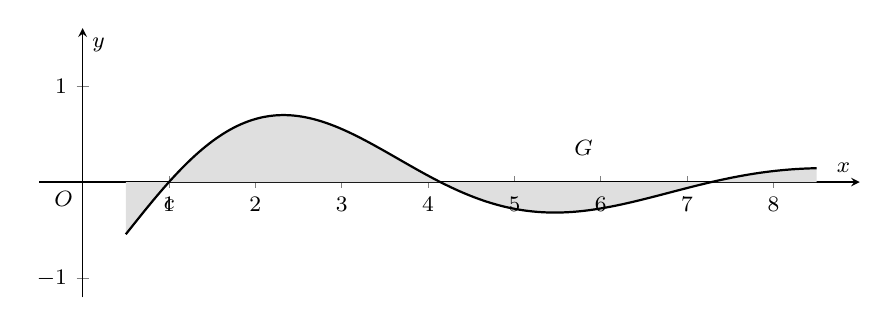
\begin{tikzpicture}
  \begin{axis}[
    axis lines=middle,
    xlabel={$x$},
    ylabel={$y$},
    xmin=-0.5, xmax=9,
    ymin=-1.2, ymax=1.6,
    xtick={1,2,3,4,5,6,7,8},
    ytick={-1,1},
    tick label style={font=\footnotesize},
    label style={font=\footnotesize},
    width=12cm,
    height=5cm,
    axis equal image=false,
    clip=false,
    samples=200,
    domain=0.5:8.5,
  ]
    % 衰减振荡曲线 y = e^{-0.25(x-1)} * sin(deg(x-1))
    \addplot[thick, name path=A] {exp(-0.25*(x-1))*sin(deg(x-1))};
    % x轴（零线）
    \path[name path=B] (axis cs:0.5,0) -- (axis cs:8.5,0);

    % 填充区域：曲线与x轴之间
    \addplot[gray!25] fill between[of=A and B];

    % 标注 c
    \node[font=\footnotesize, below] at (axis cs:1,-0.08) {$c$};
    % 标注 Γ
    \node[font=\footnotesize] at (axis cs:4.6,0.55) {$\varGamma$};
    % 标注 G
    \node[font=\footnotesize] at (axis cs:5.8,0.35) {$G$};
    % 原点 O
    \node[font=\footnotesize, below left] at (axis cs:0,0) {$O$};
  \end{axis}
\end{tikzpicture}

图 9-1
\end{center}

$b<+\infty$：广义积分 $\displaystyle\int_c^{b^-}f(x)\,dx$ 就是平面上由 $x$ 轴、直线 $x=c$ 与 $x=b$ 及函数 $f:[c,b[\to\R$ 的曲线 $\Gamma$ 所围的向正 $y$ 轴方向无限伸展的平面图形 $G$ 的“面积”（这里我们假设 $\displaystyle\lim_{x\to b^-}f(x)=+\infty$）。

若 $\displaystyle\int_c^{b^-}f(x)\,dx$ 收敛，则 $G$ 的“面积”存在且有限。

若 $\displaystyle\int_c^{b^-}f(x)\,dx$ 发散，则 $G$ 的“面积”存在但为正无穷大或负无穷大，或根本没有“面积”。

\begin{center}
	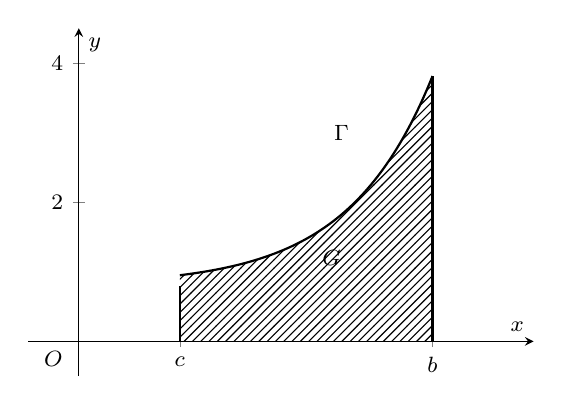
\begin{tikzpicture}[font=\footnotesize]
  \begin{axis}[
    axis lines=middle,
    xlabel={$x$},
    ylabel={$y$},
    xmin=-0.5, xmax=4.5,
    ymin=-0.5, ymax=4.5,
    xtick={1,3.5},
    xticklabels={$c$,$b$},
    ytick={},
    clip=false,
    width=8cm,
    height=6cm,
    samples=200,
  ]
    % 曲线与 x 轴之间（c 到 b）斜线填充
    \addplot[name path=A, draw=none, domain=1:3.5] {0.8 + 0.15*exp(1.2*(x-1))};
    \path[name path=B] (axis cs:1,0) -- (axis cs:3.5,0);
    \addplot[pattern=north east lines, pattern color=black] fill between[of=A and B];

    % 曲线
    \addplot[thick, domain=1:3.5] {0.8 + 0.15*exp(1.2*(x-1))};

    % 左右边界线
    \draw[thick] (axis cs:1,0) -- (axis cs:1,0.8);
    \draw[thick] (axis cs:3.5,0) -- (axis cs:3.5,{0.8+0.15*exp(1.2*2.5)});

    % 原点 O
    \node at (axis cs:-0.25,-0.25) {$O$};
    % 区域 G
    \node at (axis cs:2.5,1.2) {$G$};
    % 曲线 Γ
    \node at (axis cs:2.6,3.0) {$\Gamma$};
  \end{axis}
\end{tikzpicture}

图 9-2
\end{center}

\begin{sourceexample}{1}

考虑广义积分 $\displaystyle\int_0^{+\infty}e^{-x}\,dx$。

\end{sourceexample}

函数 $x\longmapsto e^{-x}$，$x\in[0,+\infty[$ 连续，并且
\[\lim_{d\to+\infty}\int_0^de^{-x}\,dx=\lim_{d\to+\infty}(1-e^{-d})=1,\]
因此广义积分 $\displaystyle\int_0^{+\infty}e^{-x}\,dx$ 收敛，并且
\[\int_0^{+\infty}e^{-x}\,dx=1.\]

\begin{sourceexample}{2}

考虑广义积分 $\displaystyle\int_1^{+\infty}\frac{1}{x}\,dx$。

\end{sourceexample}

函数 $x\longmapsto\dfrac{1}{x}$，$x\in[1,+\infty[$ 连续，并且
\[\lim_{d\to+\infty}\int_1^d\frac{1}{x}\,dx=\lim_{d\to+\infty}\log d=+\infty,\]
故广义积分 $\displaystyle\int_1^{+\infty}\frac{1}{x}\,dx$ 发散，但有值
\[\int_1^{+\infty}\frac{1}{x}\,dx=+\infty.\]

\begin{sourceexample}{3}

考虑广义积分 $\displaystyle\int_0^{+\infty}\cos x\,dx$。

\end{sourceexample}

函数 $x\longmapsto\cos x$，$x\in[0,+\infty[$ 连续，并且
\[\lim_{d\to+\infty}\int_0^d\cos x\,dx=\lim_{d\to+\infty}\sin d\ \text{不存在},\]
故广义积分 $\displaystyle\int_0^{+\infty}\cos x\,dx$ 不存在，从而 $\displaystyle\int_0^{+\infty}\cos x\,dx$ 发散。

\begin{sourceexample}{4}

考虑广义积分 $\displaystyle\int_0^{1^-}\frac{1}{\sqrt{1-x}}\,dx$ 与 $\displaystyle\int_0^{1^-}\frac{1}{1-x}\,dx$。

\end{sourceexample}

这里两个函数 $x\longmapsto\dfrac{1}{\sqrt{1-x}}$，$x\longmapsto\dfrac{1}{1-x}$，$x\in[0,1[$ 都连续，$x=1$ 是 $f$ 的奇点，并且
\[\lim_{c\to1^-}\int_0^c\frac{1}{\sqrt{1-x}}\,dx=\lim_{c\to1^-}\left[-2\sqrt{1-x}\right]_0^c=2-\lim_{c\to1^-}2\sqrt{1-c}=2,\]
\[\lim_{c\to1^-}\int_0^c\frac{1}{1-x}\,dx=\lim_{c\to1^-}\left[-\log(1-x)\right]_0^c=-\lim_{c\to1^-}\log(1-c)=+\infty.\]
因此广义积分 $\displaystyle\int_0^{1^-}\frac{1}{\sqrt{1-x}}\,dx$ 收敛，而广义积分 $\displaystyle\int_0^{1^-}\frac{1}{1-x}\,dx$ 发散，并且
\[\int_0^{1^-}\frac{1}{\sqrt{1-x}}\,dx=2,\quad\int_0^{1^-}\frac{1}{1-x}\,dx=+\infty.\]

\subsection{\texorpdfstring{\(\int_{a^+}^cf(x)\,dx\) 型广义积分}{a+ 到 c 型广义积分}}
	\label{sec:9-1-2}

设 $-\infty\leqslant a<c<+\infty$，函数 $f:]a,c]\to\R$ 满足下述条件：

\begin{enumerate}[label=\arabic{enumi})]
\item $f$ 在 $]a,c]$ 的任一有限闭区间 $[\alpha,\beta]$ 上可积，
\item 当 $a>-\infty$ 时，$\displaystyle\lim_{x\to a^+}f(x)=\pm\infty$（这时 $a$ 称为 $f$ 的奇点或瑕点）。
\end{enumerate}

这时，我们可以仿照 1，类似地定义 $f$ 在 $]a,c]$ 上的广义积分 $\displaystyle\int_{a^+}^cf(x)\,dx$ 为：

$\displaystyle\int_{a^+}^cf(x)\,dx$ 存在 $\Longleftrightarrow\displaystyle\lim_{d\to a^+}\int_d^cf(x)\,dx$ 存在（有限或 $\pm\infty$），并且这时
\[\int_{a^+}^cf(x)\,dx\triangleq\lim_{d\to a^+}\int_d^cf(x)\,dx,\]
$\displaystyle\int_{a^+}^cf(x)\,dx$ 收敛 $\Longleftrightarrow\displaystyle\lim_{d\to a^+}\int_d^cf(x)\,dx$ 有限，
$\displaystyle\int_{a^+}^cf(x)\,dx$ 发散 $\Longleftrightarrow\displaystyle\lim_{d\to a^+}\int_d^cf(x)\,dx$ 不存在或为 $\pm\infty$。

①当 $a=-\infty$ 时，$d\to a^+$ 就是 $d\to-\infty$，以下同。

\begin{sourceexample}{5}

考虑广义积分 $\displaystyle\int_{0^+}^1\log x\,dx$。

\end{sourceexample}

这里函数 $x\longmapsto\log x$，$x\in\ ]0,1]$ 连续，$x=0$ 是它的唯一奇点，由于
\[\lim_{d\to0^+}\int_d^1\log x\,dx=\lim_{d\to0^+}\left([x\log x]_d^1-\int_d^1dx\right)=-1,\]
故广义积分 $\displaystyle\int_{0^+}^1\log x\,dx$ 收敛，其值
\[\int_{0^+}^1\log x\,dx=-1.\]

\begin{sourceexample}{6}

考虑广义积分 $\displaystyle\int_{-\infty}^0e^{-x}\cos x\,dx$。

\end{sourceexample}

这里函数 $x\longmapsto e^{-x}\cos x$，$x\in\ ]-\infty,0]$ 连续。$\forall\,d<0$，直接计算得到
\[\int_d^0e^{-x}\cos x\,dx=\frac{1}{2}e^{-d}(-\sin d+\cos d)-\frac{1}{2}.\]
由此可知，极限 $\displaystyle\lim_{d\to-\infty}\int_d^0e^{-x}\cos x\,dx$ 不存在，因此广义积分 $\displaystyle\int_{-\infty}^0e^{-x}\cos x\,dx$ 不存在，从而发散。

\subsection{\texorpdfstring{\(\int_{a^+}^{b^-}f(x)\,dx\) 型广义积分}{a+ 到 b- 型广义积分}}

设 $-\infty\leqslant a<b\leqslant+\infty$，假设函数 $f:]a,b[\to\R$ 满足下述条件：

\begin{enumerate}[label=\arabic{enumi})]
\item $f$ 在 $]a,b[$ 的任一有限闭区间 $[\alpha,\beta]$ 上可积，
\item 当 $a>-\infty$，$b<+\infty$ 时，$\displaystyle\lim_{x\to a^+}f(x)=\pm\infty$，$\displaystyle\lim_{x\to b^-}f(x)=\pm\infty$（即 $a,b$ 是 $f$ 的奇点或瑕点）。
\end{enumerate}

现在我们假设对某一 $c\in\ ]a,b[$，广义积分之和 $\displaystyle\int_{a^+}^cf(x)\,dx+\int_c^{b^-}f(x)\,dx\in\overline{\R}$。于是由定义可推知下面两个简单结论成立：

\begin{enumerate}[label=\arabic{enumi})]
\item $\forall\,c'\in\ ]a,b[$，都有
\[\int_{a^+}^{c'}f(x)\,dx+\int_{c'}^{b^-}f(x)\,dx\in\overline{\R}.\]
\item 对任意 $c,c'\in\ ]a,b[$，都有
\[\int_{a^+}^{c}f(x)\,dx+\int_{c}^{b^-}f(x)\,dx=\int_{a^+}^{c'}f(x)\,dx+\int_{c'}^{b^-}f(x)\,dx.\]
\end{enumerate}

第二式表明 $\displaystyle\int_{a^+}^cf(x)\,dx+\int_c^{b^-}f(x)\,dx$ 的值与 $c$ 的选择无关，因此我们引入下述定义。

\begin{mydef*}{}

设函数 $f:]a,b[\to\R$ 满足上面所述条件，则 $f$ 在 $]a,b[$ 上的广义积分，记为 $\displaystyle\int_{a^+}^{b^-}f(x)\,dx$，定义如下：

\begin{enumerate}[label=\arabic{enumi})]
\item $\displaystyle\int_{a^+}^{b^-}f(x)\,dx$ 存在，当且仅当对某一 $c\in\ ]a,b[$，
\[\int_{a^+}^{c}f(x)\,dx+\int_c^{b^-}f(x)\,dx\]
是有限实数或 $\pm\infty$。并且这时
\[\int_{a^+}^{b^-}f(x)\,dx\triangleq\int_{a^+}^{c}f(x)\,dx+\int_{c}^{b^-}f(x)\,dx.\]
\item $\displaystyle\int_{a^+}^{b^-}f(x)\,dx$ 收敛，当且仅当对某一 $c\in\ ]a,b[$，$\displaystyle\int_{a^+}^{c}f(x)\,dx$ 与 $\displaystyle\int_c^{b^-}f(x)\,dx$ 收敛。
\item $\displaystyle\int_{a^+}^{b^-}f(x)\,dx$ 发散，当且仅当对某一 $c\in\ ]a,b[$，$\displaystyle\int_{a^+}^{c}f(x)\,dx$ 与 $\displaystyle\int_c^{b^-}f(x)\,dx$ 中至少有一个发散。特别地，若 $\displaystyle\int_{a^+}^{c}f(x)\,dx=+\infty\,(-\infty)$，$\displaystyle\int_c^{b^-}f(x)\,dx=-\infty\,(+\infty)$；或 $\displaystyle\int_{a^+}^{c}f(x)\,dx$ 与 $\displaystyle\int_c^{b^-}f(x)\,dx$ 中有一个不存在，则我们称 $\displaystyle\int_{a^+}^{b^-}f(x)\,dx$ 不存在。
\end{enumerate}

\end{mydef*}

\begin{sourceexample}{7}

考虑广义积分 $\displaystyle\int_{-1^+}^{1^-}\frac{1}{\sqrt{1-x^2}}\,dx$。

\end{sourceexample}

这里函数 $x\longmapsto\dfrac{1}{\sqrt{1-x^2}}$，$x\in\ ]-1,1[$ 连续，并且 $x=\pm1$ 是它的两个奇点。由于
\[\lim_{d\to-1^+}\int_d^0\frac{1}{\sqrt{1-x^2}}\,dx+\lim_{d'\to1^-}\int_0^{d'}\frac{1}{\sqrt{1-x^2}}\,dx\]
\[=\lim_{d\to-1^+}(-\arcsin d)+\lim_{d'\to1^-}(\arcsin d')=\frac{\pi}{2}+\frac{\pi}{2}=\pi,\]
故广义积分 $\displaystyle\int_{-1^+}^{1^-}\frac{1}{\sqrt{1-x^2}}\,dx$ 收敛，并且
\[\int_{-1^+}^{1^-}\frac{1}{\sqrt{1-x^2}}\,dx=\pi.\]

\begin{sourceexample}{8}

考虑广义积分 $\displaystyle\int_{-\infty}^{+\infty}\frac{1+x}{1+x^2}\,dx$。

\end{sourceexample}

这里函数 $x\longmapsto\dfrac{1+x}{1+x^2}$，$x\in\ ]-\infty,+\infty[$ 连续，由于
\[\int_0^{+\infty}\frac{1+x}{1+x^2}\,dx=\lim_{d\to+\infty}\int_0^d\frac{1+x}{1+x^2}\,dx\]
\[=\lim_{d\to+\infty}\left(\left[\operatorname{arctg}x\right]_0^d+\frac{1}{2}\left[\log(1+x^2)\right]_0^d\right)\]
\[=\lim_{d\to+\infty}\left(\operatorname{arctg}d+\frac{1}{2}\log(1+d^2)\right)\]
\[=+\infty,\]
故广义积分 $\displaystyle\int_{-\infty}^{+\infty}\frac{1+x}{1+x^2}\,dx$ 发散，并且由于
\[\int_{-\infty}^{0}\frac{1+x}{1+x^2}\,dx=\lim_{c\to-\infty}\int_c^0\frac{1+x}{1+x^2}\,dx\]
\[=\lim_{c\to-\infty}\left(\left[\operatorname{arctg}x\right]_c^0+\frac{1}{2}\left[\log(1+x^2)\right]_c^0\right)\]
\[=\lim_{c\to-\infty}\left(-\operatorname{arctg}c-\frac{1}{2}\log(1+c^2)\right)=-\infty,\]
故广义积分 $\displaystyle\int_{-\infty}^{+\infty}\frac{1+x}{1+x^2}\,dx$ 实际上不存在。

附注 1 如果我们在例 8 的第 2 个积分 $\displaystyle\int_{-\infty}^{0}\frac{1+x}{1+x^2}\,dx$ 计算过程中取 $c=-d$，并与第一个积分的极限计算过程合并在一起，则出现下述情形：
\[\lim_{d\to+\infty}\left(\int_{-d}^{0}\frac{1+x}{1+x^2}\,dx+\int_{0}^{d}\frac{1+x}{1+x^2}\,dx\right)\]
\[=\lim_{d\to+\infty}\left(\left[\operatorname{arctg}x\right]_{-d}^{d}+\frac{1}{2}\left[\log(1+x^2)\right]_{-d}^{d}\right)\]
\[=\lim_{d\to+\infty}2\operatorname{arctg}d=\pi.\]
由此似乎应推得
\[\int_{-\infty}^{+\infty}\frac{1+x}{1+x^2}\,dx=\pi\]
其实不然，因为根据广义积分 $\displaystyle\int_{a^+}^{b^-}f(x)\,dx$ 的定义，
\[\int_{-\infty}^{0}\frac{1+x}{1+x^2}\,dx+\int_{0}^{+\infty}\frac{1+x}{1+x^2}\,dx=\lim_{c\to-\infty}\int_{c}^{0}\frac{1+x}{1+x^2}\,dx+\lim_{d\to+\infty}\int_{0}^{d}\frac{1+x}{1+x^2}\,dx\]
的右边 $c\to-\infty$ 与 $d\to+\infty$ 是两个完全独立的极限过程，而在上面我们的计算 $\displaystyle\lim_{d\to+\infty}\left(\int_{-d}^{0}\frac{1+x}{1+x^2}\,dx+\int_{0}^{d}\frac{1+x}{1+x^2}\,dx\right)$ 中，已经通过令 $c=-d$ 而化为 $d\to+\infty$ 的一个极限过程，从而出现两种截然不同的结果。

为了区别这种情形，我们特作下述定义。

\begin{mydef*}{}

对于广义积分 $\displaystyle\int_{a^+}^{b^-}f(x)\,dx$，

\begin{enumerate}[label=\arabic{enumi})]
\item 若 $a=-\infty$，$b=+\infty$：则 $f$ 在 $]-\infty,+\infty[$ 上的 Cauchy 广义积分主值，记为 $(C)\displaystyle\int_{-\infty}^{+\infty}f(x)\,dx$，定义为：
\[(C)\int_{-\infty}^{+\infty}f(x)\,dx=\lim_{d\to+\infty}\int_{-d}^{d}f(x)\,dx.\]
\item 若 $a>-\infty$，$b<+\infty$：则 $f$ 在 $]a,b[$ 上的 Cauchy 广义积分主值，记为 $(C)\displaystyle\int_{a^+}^{b^-}f(x)\,dx$，定义为：
\[(C)\int_{a^+}^{b^-}f(x)\,dx=\lim_{\eta\to0^+}\int_{a+\eta}^{b-\eta}f(x)\,dx.\]
\end{enumerate}

\end{mydef*}

由上述定义可知，若广义积分 $\displaystyle\int_{a^+}^{b^-}f(x)\,dx$ 收敛则它的值就是 Cauchy 广义积分主值 $(C)\displaystyle\int_{a^+}^{b^-}f(x)\,dx$。

于是我们有
\[\int_{-1^+}^{1^-}\frac{1}{\sqrt{1-x^2}}\,dx=(C)\int_{-1^+}^{1^-}\frac{1}{\sqrt{1-x^2}}\,dx=\pi,\]
\[\int_{-\infty}^{+\infty}\frac{1+x}{1+x^2}\,dx\text{ 发散，但 }(C)\int_{-\infty}^{+\infty}\frac{1+x}{1+x^2}\,dx=\pi.\]

附注 2 如果出现下述形式的两个广义积分：
\[\int_{a}^{c^-}f(x)\,dx,\ \int_{c^+}^{b}f(x)\,dx\quad(\text{这里 }a>-\infty,\ b<+\infty,\ c\in\R)\]
则它们的和 $\displaystyle\int_{a}^{c^-}f(x)\,dx+\int_{c^+}^{b}f(x)\,dx$，记为 $\displaystyle\int_{a}^{b}f(x)\,dx$，自然应作如下规定：

\begin{enumerate}[label=\arabic{enumi})]
\item 广义积分 $\displaystyle\int_a^bf(x)\,dx$ 存在 $\Longleftrightarrow\displaystyle\int_a^{c^-}f(x)\,dx+\int_{c^+}^bf(x)\,dx$ 为有限实数或 $\pm\infty$，
并且这时
\[\int_a^bf(x)\,dx\triangleq\int_a^{c^-}f(x)\,dx+\int_{c^+}^bf(x)\,dx.\]
\item 广义积分 $\displaystyle\int_a^bf(x)\,dx$ 收敛 $\Longleftrightarrow\displaystyle\int_a^{c^-}f(x)\,dx$ 与 $\displaystyle\int_{c^+}^bf(x)\,dx$ 收敛。
\item 广义积分 $\displaystyle\int_a^bf(x)\,dx$ 发散 $\Longleftrightarrow\displaystyle\int_a^{c^-}f(x)\,dx$ 与 $\displaystyle\int_{c^+}^bf(x)\,dx$ 中至少有一个发散。
\item 广义积分 $\displaystyle\int_a^bf(x)\,dx$ 的 Cauchy 广义积分主值
\[(C)\int_a^bf(x)\,dx\triangleq\lim_{\eta\to0^+}\left(\int_a^{c-\eta}f(x)\,dx+\int_{c+\eta}^bf(x)\,dx\right).\]
\end{enumerate}

此外，我们还可以将这种广义积分 $\displaystyle\int_a^bf(x)\,dx$ 推广到 $f$ 在 $]a,b[$ 上有有限个奇点的情形上去。具体的叙述留给读者。

\begin{sourceexample}{9}

考虑广义积分 $\displaystyle\int_0^2\frac{x}{\sqrt{|1-x^2|}}\,dx$。

\end{sourceexample}

这里函数 $x\longmapsto\dfrac{x}{\sqrt{|1-x^2|}}$，$x\in[0,2]-\{1\}$ 连续，并且 $x=1$ 是它的唯一奇点。由于
\[\int_0^{1^-}\frac{x}{\sqrt{|1-x^2|}}\,dx=\lim_{c\to1^-}\int_0^c\frac{x}{\sqrt{1-x^2}}\,dx=1,\]
\[\int_{1^+}^2\frac{x}{\sqrt{|1-x^2|}}\,dx=\lim_{d\to1^+}\int_d^2\frac{x}{\sqrt{x^2-1}}\,dx=\sqrt{3},\]
故广义积分 $\displaystyle\int_0^2\frac{x}{\sqrt{|1-x^2|}}\,dx$ 收敛，并且
\[\int_0^2\frac{x}{\sqrt{|1-x^2|}}\,dx=\int_0^{1^-}\frac{x}{\sqrt{|1-x^2|}}\,dx+\int_{1^+}^2\frac{x}{\sqrt{|1-x^2|}}\,dx\]
\[=1+\sqrt{3}.\]

\begin{sourceexample}{10}

考虑广义积分 $\displaystyle\int_{-1}^{1}\frac{1}{x}\,dx$。

\end{sourceexample}

此函数 $x\longmapsto\dfrac{1}{x}$，$x\in[-1,1]-\{0\}$ 连续，$x=0$ 是它的唯一奇点。由于
\[\int_{-1}^{0^-}\frac{1}{x}\,dx=\lim_{c\to0^-}\int_{-1}^{c}\frac{1}{x}\,dx=-\infty,\]
\[\int_{0^+}^{1}\frac{1}{x}\,dx=\lim_{d\to0^+}\int_{d}^{1}\frac{1}{x}\,dx=+\infty,\]
故广义积分 $\displaystyle\int_{-1}^{1}\frac{1}{x}\,dx$ 不存在，但是它的 Cauchy 广义积分主值
\[(C)\int_{-1}^{1}\frac{1}{x}\,dx=\lim_{\eta\to0^+}\left(\int_{-1}^{-\eta}\frac{1}{x}\,dx+\int_{\eta}^{1}\frac{1}{x}\,dx\right)\]
\[=0.\]

\subsection{广义积分的两个计算方法}
	\label{sec:9-1-4}

对广义积分，也有类似于普通 Riemann 积分的变元替换法与分部积分法。下面我们只对 $\displaystyle\int_{a}^{b^-}f(x)\,dx$ 型广义积分叙述这两个计算方法，对另外两种类型的广义积分，读者可以自己补充。

\begin{mythm}{变元替换法}{substitution-improper}

设函数 $\varphi:[\alpha,\beta[\to\R$ 在 $[\alpha,\beta[$ 上是 $C^1$ 类的，$I\subset\R$ 是包含 $\varphi([\alpha,\beta[)$ 的一个区间，函数 $f:I\to\R$ 在 $I$ 上连续。那末广义积分 $\displaystyle\int_{\alpha}^{\beta^-}f(\varphi(t))\varphi'(t)\,dt$ 收敛，当且仅当极限
\[\lim_{s\to\beta^-}\int_{\varphi(\alpha)}^{\varphi(s)}f(x)\,dx\]
存在并且有限。并且这时
\[\int_{\alpha}^{\beta^-}f(\varphi(t))\varphi'(t)\,dt=\lim_{s\to\beta^-}\int_{\varphi(\alpha)}^{\varphi(s)}f(x)\,dx.\]

\end{mythm}

\begin{proof}

设 $s\in[\alpha,\beta[$，根据定积分的变元替换法（\rthm{thm:substitution-rule} 推论）我们有
\[\int_{\alpha}^{s}f(\varphi(t))\varphi'(t)\,dt=\int_{\varphi(\alpha)}^{\varphi(s)}f(x)\,dx.\]
两边令 $s\to\beta^-$ 取极限即得。$\blacksquare$

\end{proof}

\begin{sourceexample}{11}

计算广义积分 $\displaystyle\int_0^{+\infty}\frac{\operatorname{arctg}x}{(1+x^2)^{3/2}}\,dx$。

\end{sourceexample}

令 $x=\varphi(t)=\operatorname{tg}t$，$t\in\left[0,\dfrac{\pi}{2}\right[$。显然 $\varphi$ 在 $\left[0,\dfrac{\pi}{2}\right[$ 上是 $C^1$ 类的，并且 $[0,+\infty[=\varphi\left(\left[0,\dfrac{\pi}{2}\right[\right)$。由于函数
\[x\longmapsto f(x)=\frac{\operatorname{arctg}x}{(1+x^2)^{3/2}},\quad x\in[0,+\infty[\]
在 $[0,+\infty[$ 上连续，故由上述定理知，
\[\int_0^{+\infty}\frac{\operatorname{arctg}x}{(1+x^2)^{3/2}}\,dx\text{ 收敛}\Longleftrightarrow\int_0^{\frac{\pi}{2}}\frac{\operatorname{arctg}(\operatorname{tg}t)}{(1+\operatorname{tg}^2t)^{3/2}}(\operatorname{tg}t)'\,dt\text{ 收敛。}\]
这里
\[\int_0^{\frac{\pi}{2}}\frac{\operatorname{arctg}(\operatorname{tg}t)}{(1+\operatorname{tg}^2t)^{3/2}}(\operatorname{tg}t)'\,dt=\int_0^{\frac{\pi}{2}}t\cos t\,dt,\]
显然收敛，因此
\[\int_0^{+\infty}\frac{\operatorname{arctg}x}{(1+x^2)^{3/2}}\,dx=\int_0^{\frac{\pi}{2}}t\cos t\,dt\]
\[=\left[t\sin t\right]_0^{\frac{\pi}{2}}-\int_0^{\frac{\pi}{2}}\sin t\,dt\]
\[=\frac{\pi}{2}-1.\]

\begin{mythm}{分部积分法}{integration-by-parts-improper}

设函数 $u,v:[c,b[\to\R$ 在 $[c,b[$ 上是 $C^1$ 类的，如果

\begin{enumerate}[label=\arabic{enumi})]
\item $\displaystyle\lim_{x\to b^-}u(x)v(x)$ 存在并且有限，
\item 广义积分 $\displaystyle\int_{c}^{b^-}u'(x)v(x)\,dx$ 收敛，
\end{enumerate}

则广义积分 $\displaystyle\int_{c}^{b^-}u(x)v'(x)\,dx$ 也收敛，并且
\[\int_{c}^{b^-}u(x)v'(x)\,dx=\lim_{x\to b^-}\left[u(x)v(x)-u(c)v(c)\right]-\int_{c}^{b^-}u'(x)v(x)\,dx.\]

\end{mythm}

\begin{proof}

设 $d\in[c,b[$，由定积分的分部积分法（\rthm{thm:integration-by-parts} 推论）我们有
\[\int_{c}^{d}u(x)v'(x)\,dx=u(d)v(d)-u(c)v(c)-\int_{c}^{d}u'(x)v(x)\,dx.\]
两边令 $d\to b^-$ 取极限，由定理假设知左边极限 $\displaystyle\lim_{d\to b^-}\int_{c}^{d}u(x)v'(x)\,dx$ 存在并且有限，故广义积分 $\displaystyle\int_{c}^{b^-}u(x)v'(x)\,dx$ 收敛，并且定理的等式成立。

习惯上我们把上述等式写成下述形式：
\[\int_{c}^{b^-}u(x)v'(x)\,dx=\left[u(x)v(x)\right]_{c}^{b^-}-\int_{c}^{b^-}u'(x)v(x)\,dx.\]

\end{proof}

\begin{sourceexample}{12}

计算广义积分 $\displaystyle\int_1^{+\infty}\frac{\log x}{x^2}\,dx$。

\end{sourceexample}

由于
\[\int_1^{+\infty}\frac{\log x}{x^2}\,dx=\int_1^{+\infty}\log x\cdot\left(-\frac{1}{x}\right)'dx,\]
若令函数 $u,v:[1,+\infty[\to\R$ 为
\[\forall\,x\in[1,+\infty[,\quad u(x)=\log x,\ v(x)=-\frac{1}{x}.\]
则 $u,v$ 满足分部积分法的两个条件，因此广义积分 $\displaystyle\int_1^{+\infty}\frac{\log x}{x^2}\,dx$ 收敛，并且
\[\int_1^{+\infty}\frac{\log x}{x^2}\,dx=\left[-\frac{1}{x}\log x\right]_1^{+\infty}-\int_1^{+\infty}\left(-\frac{1}{x}\right)(\log x)'dx\]
\[=\int_1^{+\infty}\frac{1}{x^2}\,dx\]
\[=1.\]

\subsection{两个重要的广义积分}

下面两个广义积分对判断一般广义积分的收敛与发散性将起着重要作用，我们把它们作为一个命题列出。

\begin{myprop*}{}

对广义积分 $\displaystyle\int_{0^+}^1\frac{1}{x^{\lambda}}\,dx$ 与 $\displaystyle\int_1^{+\infty}\frac{1}{x^{\lambda}}\,dx$ 下述结论成立：

\begin{enumerate}[label=\arabic{enumi})]
\item $\displaystyle\int_{0^+}^1\frac{1}{x^{\lambda}}\,dx\begin{cases} \text{收敛，若 }\lambda<1;\\ \text{发散，若 }\lambda\geqslant1. \end{cases}$
\item $\displaystyle\int_1^{+\infty}\frac{1}{x^{\lambda}}\,dx\begin{cases} \text{收敛，若 }\lambda>1;\\ \text{发散，若 }\lambda\leqslant1. \end{cases}$
\end{enumerate}

\end{myprop*}

\begin{proof}

直接利用定义计算这两个积分，即可验证命题成立。

\end{proof}

最后作为这一节的结束，我们特作如下说明。

\textbf{记号说明}\quad 为了书写简单起见，今后对广义积分 $\displaystyle\int_a^{b^-}f(x)\,dx$、$\displaystyle\int_{a^+}^bf(x)\,dx$ 及 $\displaystyle\int_{a^+}^{b^-}f(x)\,dx$，如无特别指明需要，我们一律删去上标“$+$”与“$-$”，读者从 $\displaystyle\int_a^bf(x)\,dx$ 的具体形式可以明了它是普通 Riemann 积分还是广义积分。

\subsection*{习 题}

\begin{exercise}
	\item 计算下列各广义积分：
	\begin{enumerate}[label=\arabic*)]
		\item $\displaystyle\int_0^1\frac{x\log x}{(1+x^2)^2}\,dx$；
		\item $\displaystyle\int_0^{+\infty}\frac{x^2+1}{x^4+1}\,dx$；
		\item $\displaystyle\int_0^{+\infty}\frac{1}{1+x^4}\,dx$；
		\item $\displaystyle\int_a^b\frac{1}{\sqrt{(x-a)(b-x)}}\,dx$；
		\item $\displaystyle\int_0^1\frac{1}{x\sqrt{1+x^2}}\,dx$；
		\item $\displaystyle\int_0^{+\infty}\frac{x^2\log x}{(1+x^4)^3}\,dx$。
	\end{enumerate}
\end{exercise}

\begin{exercise}
	\item
	\begin{enumerate}[label=\arabic*)]
		\item 证明：广义积分 $\displaystyle\int_0^{+\infty}\frac{x-2}{x^3-1}\,dx$ 不存在。
		\item 证明：广义积分 $\displaystyle\int_1^{+\infty}\operatorname{arctg}\frac{1}{x}\,dx$ 存在但不收敛。
		\item 证明：广义积分 $\displaystyle\int_1^{+\infty}\frac{x\log\left(1+\dfrac{1}{x}\right)}{1+x^2}\,dx$ 收敛。
	\end{enumerate}
\end{exercise}

\begin{exercise}
	\item 计算下列各 Cauchy 广义积分主值：
	\begin{enumerate}[label=\arabic*)]
		\item $(C)\displaystyle\int_0^{+\infty}\frac{1}{1-x^2}\,dx$；
		\item $(C)\displaystyle\int_0^4\frac{1}{x^2-4x+3}\,dx$；
		\item $(C)\displaystyle\int_{-\infty}^{+\infty}\sin x\,dx$；
		\item $(C)\displaystyle\int_{1/2}^2\frac{1}{x\log x}\,dx$。
	\end{enumerate}
\end{exercise}

\begin{exercise}
	\item 计算广义积分 $I=\displaystyle\int_0^{+\infty}\frac{1}{(1+x^2)(1+x^{\lambda})}\,dx$ $(\lambda\geqslant0)$。
\end{exercise}

\begin{exercise}
	\item 计算下列各广义积分：
	\begin{enumerate}[label=\arabic*)]
		\item $\displaystyle\int_0^{+\infty}\frac{\log x}{1+x}\,dx$；
		\item $\displaystyle\int_0^{+\infty}\frac{\log x}{(1+x^2)^2}\,dx$；
		\item $\displaystyle\int_0^{\pi}\log(1+\cos\theta)\,d\theta$；
		\item $\displaystyle\int_0^{+\infty}\log\left(x+\frac{1}{x}\right)\frac{1}{1+x^2}\,dx$；
		\item $\displaystyle\int_{-1}^{1}\frac{x^3}{\sqrt{1-x^2}}\log\frac{1+x}{1-x}\,dx$；
		\item $\displaystyle\int_0^1\frac{1}{(1+x)^{3/2}\sqrt{x(1-x)}}\,dx$。
	\end{enumerate}
\end{exercise}

\section{广义积分的收敛准则}

在上一节，我们研究了三类广义积分：

\begin{enumerate}[label=\roman{enumi})]
\item $\displaystyle\int_a^{b^-}f(x)\,dx$；
\item $\displaystyle\int_{a^+}^bf(x)\,dx$；
\item $\displaystyle\int_{a^+}^{b^-}f(x)\,dx$。
\end{enumerate}

第 iii) 类广义积分 $\displaystyle\int_{a^+}^{b^-}f(x)\,dx$ 实际上是第 i) 类与第 ii) 类广义积分的组合。

第 ii) 类广义积分 $\displaystyle\int_{a^+}^cf(x)\,dx$ 可通过变元替换 $x=-y$ 化为第 i) 类广义积分。因为我们有
\[\int_{a^+}^cf(x)\,dx=-\int_{(-a)^-}^{-c}f(-y)\,dy=\int_{-c}^{(-a)^-}f(-y)\,dy.\]
因此要研究一般广义积分的收敛与发散性，实际上我们只需研究第 i) 类型的广义积分 $\displaystyle\int_a^{b^-}f(x)\,dx$ 的收敛与发散性。

下面我们就来研究广义积分 $\displaystyle\int_a^{b^-}f(x)\,dx$ 的收敛性与发散性。

\subsection{广义积分的一般收敛准则}
	\label{sec:9-2-1}

\begin{mythm}{}{improper-linear}

设 $\displaystyle\int_a^{b^-}f(x)\,dx$ 与 $\displaystyle\int_a^{b^-}g(x)\,dx$ 是任意两个广义积分。

\begin{enumerate}[label=\arabic{enumi})]
\item 若 $\displaystyle\int_a^{b^-}f(x)\,dx$ 与 $\displaystyle\int_a^{b^-}g(x)\,dx$ 收敛，则广义积分 $\displaystyle\int_a^{b^-}[f(x)+g(x)]\,dx$ 也收敛，并且
\[\int_a^{b^-}[f(x)+g(x)]\,dx=\int_a^{b^-}f(x)\,dx+\int_a^{b^-}g(x)\,dx.\]
\item 若 $\displaystyle\int_a^{b^-}f(x)\,dx$ 收敛，则 $\forall\,\lambda\in\R$，广义积分 $\displaystyle\int_a^{b^-}(\lambda f)(x)\,dx$ 也收敛，并且
\[\int_a^{b^-}(\lambda f)(x)\,dx=\lambda\int_a^{b^-}f(x)\,dx.\]
\end{enumerate}

\end{mythm}

\begin{proof}

直接由广义积分的定义及函数极限的性质推出。

\end{proof}

\begin{mythm}{Cauchy收敛准则}{cauchy-improper}

广义积分 $\displaystyle\int_a^{b^-}f(x)\,dx$ 收敛的充分必要条件是：
\[(\forall\,\varepsilon>0)(\exists\,B\geqslant a)(\forall\,c,c'\geqslant B)\Longrightarrow\left|\int_c^{c'}f(x)\,dx\right|<\varepsilon.\]

\end{mythm}

\begin{proof}

因为广义积分 $\displaystyle\int_a^{b^-}f(x)\,dx$ 收敛当且仅当函数 $F:[a,b[\to\R$（$\forall\,c\in[a,b[$，$F(c)=\displaystyle\int_a^cf(x)\,dx$）当 $c\to b^-$ 时有有限的极限存在，而 $\forall\,c,c'\geqslant a$，
\[F(c)-F(c')=\int_c^{c'}f(x)\,dx.\]
因此上述广义积分 $\displaystyle\int_a^{b^-}f(x)\,dx$ 收敛的充要条件正好就是函数 $F$ 当 $c\to b^-$ 的 Cauchy 收敛准则。从而定理成立。

\end{proof}

\begin{mythm}{比较判别法}{comparison-improper}

设 $\displaystyle\int_a^{b^-}f(x)\,dx$ 与 $\displaystyle\int_a^{b^-}g(x)\,dx$ 是任意两个广义积分，函数 $f,g:[a,b[\to\R$ 满足下述不等式：
\[\forall\,x\in[a,b[,\quad 0\leqslant f(x)\leqslant g(x).\]
\begin{enumerate}[label=\arabic{enumi})]
\item 若 $\displaystyle\int_a^{b^-}g(x)\,dx$ 收敛，则 $\displaystyle\int_a^{b^-}f(x)\,dx$ 也收敛，并且
\[\int_a^{b^-}f(x)\,dx\leqslant\int_a^{b^-}g(x)\,dx.\]
\item 若 $\displaystyle\int_a^{b^-}f(x)\,dx$ 发散，则 $\displaystyle\int_a^{b^-}g(x)\,dx$ 也发散。
\end{enumerate}

\end{mythm}

\begin{proof}

因为 $\forall\,x\in[a,b[$，$0\leqslant f(x)\leqslant g(x)$，所以
\[\forall\,c\in[a,b[,\quad 0\leqslant\int_a^cf(x)\,dx\leqslant\int_a^cg(x)\,dx.\]
1) 若 $\displaystyle\int_a^{b^-}g(x)\,dx$ 收敛，则由于函数 $c\longmapsto F(c)=\displaystyle\int_a^cf(x)\,dx$，$c\in[a,b[$ 关于 $c$ 单调上升，并且
\[\int_a^cf(x)\,dx\leqslant\int_a^cg(x)\,dx\leqslant\int_a^{b^-}g(x)\,dx<+\infty,\]
故极限 $\displaystyle\lim_{c\to b^-}F(c)$ 存在且有限，从而广义积分 $\displaystyle\int_a^{b^-}f(x)\,dx$ 收敛。

2) 若 $\displaystyle\int_a^{b^-}f(x)\,dx$ 发散，则由反证法及结论 1) 知，广义积分 $\displaystyle\int_a^{b^-}g(x)\,dx$ 必然发散。

\end{proof}

\begin{mycor*}{}

若函数 $f,g:[a,b[\to\R$ 满足条件：$f\geqslant0$，$g\geqslant0$ 并且 $f(x)\sim g(x)\ (x\to b^-)$，
则广义积分 $\displaystyle\int_a^{b^-}f(x)\,dx$ 与 $\displaystyle\int_a^{b^-}g(x)\,dx$ 有相同的收敛与发散性。

\end{mycor*}

\begin{proof}

因为 $f(x)\sim g(x)\ (x\to b^-)$，所以存在 $B$，$a\leqslant B<b$ 使得
\[\frac{1}{2}g(x)\leqslant f(x)\leqslant2g(x),\quad\forall\,x\in[B,b[.\]
由此不等式及上述比较判别法立即推知此推论成立。

\end{proof}

\begin{sourceexample}{1}

考虑广义积分 $\displaystyle\int_1^{+\infty}\frac{\log x}{\sqrt{x}}\,dx$。

\end{sourceexample}

由于函数 $x\longmapsto\dfrac{\log x}{\sqrt{x}}$，$x\in[1,+\infty[$ 在 $[1,+\infty[$ 上连续，并且
\[\forall\,x\geqslant e,\quad\frac{\log x}{\sqrt{x}}\geqslant\frac{1}{\sqrt{x}},\]
而广义积分 $\displaystyle\int_1^{+\infty}\frac{1}{\sqrt{x}}\,dx$ 发散，故由比较判别法知，广义积分
\[\int_1^{+\infty}\frac{\log x}{\sqrt{x}}\,dx\]
发散。

\begin{sourceexample}{2}

考虑广义积分 $\displaystyle\int_1^{+\infty}\frac{x}{\sqrt{x^5+x+1}}\,dx$。

\end{sourceexample}

函数 $x\longmapsto\dfrac{x}{\sqrt{x^5+x+1}}$，$x\in[1,+\infty[$ 在 $[1,+\infty[$ 上连续，并且由于
\[x^5+x+1=x^5\left(1+\frac{1}{x^4}+\frac{1}{x^5}\right)\sim x^5\quad(x\to+\infty);\]
故
\[\frac{x}{\sqrt{x^5+x+1}}\sim x\cdot x^{-\frac{5}{2}}=\frac{1}{x^{3/2}}\quad(x\to+\infty).\]
广义积分 $\displaystyle\int_1^{+\infty}\frac{1}{x^{3/2}}\,dx$ 收敛；故由上述推论知，广义积分
\[\int_1^{+\infty}\frac{x}{\sqrt{x^5+x+1}}\,dx\]
收敛。

\begin{sourceexample}{3}

考虑广义积分 $\displaystyle\int_0^{1^-}\frac{1}{\sqrt[4]{1-x^4}}\,dx$。

\end{sourceexample}

$x=1$ 是此广义积分的唯一奇点。并且
\[\frac{1}{\sqrt[4]{1-x^4}}=1/[1-(x-1+1)^4]^{\frac{1}{4}}\]
\[=1/[4(1-x)-6(1-x)^2+4(1-x)^3-(1-x)^4]^{\frac{1}{4}}\]
\[=1/\left(\sqrt[4]{4}(1-x)^{\frac{1}{4}}\left[1-\frac{6}{4}(1-x)+(1-x)^2-\frac{1}{4}(1-x)^3\right]^{\frac{1}{4}}\right)\]
\[\sim\frac{1}{\sqrt[4]{4}(1-x)^{\frac{1}{4}}}\quad(x\to1^-).\]
而广义积分 $\displaystyle\int_0^{1^-}\frac{1}{(1-x)^{\frac{1}{4}}}\,dx$ 收敛，故广义积分 $\displaystyle\int_0^{1^-}\frac{1}{\sqrt[4]{1-x^4}}\,dx$ 收敛。

\begin{sourceexample}{4}

考虑广义积分 $\displaystyle\int_0^{+\infty}\frac{1}{x^{\alpha}(1+x^{\beta})}\,dx$ $(\alpha,\beta\in\R)$。

\end{sourceexample}

$\forall\,\alpha,\beta\in\R$，函数 $x\longmapsto\dfrac{1}{x^{\alpha}(1+x^{\beta})}$，$x\in[1,+\infty[$ 在 $[1,+\infty[$ 上连续。

\begin{enumerate}[label=\arabic{enumi})]
\item $\beta\leqslant0$：这时
\[\frac{1}{x^{\alpha}(1+x^{\beta})}\sim\frac{1}{x^{\alpha}}\quad(x\to+\infty),\ \text{若 }\beta<0,\]
\[\frac{1}{x^{\alpha}(1+x^{\beta})}\sim\frac{1}{2x^{\alpha}}\quad(x\to+\infty),\ \text{若 }\beta=0.\]
因此广义积分 $\displaystyle\int_1^{+\infty}\frac{1}{x^{\alpha}(1+x^{\beta})}\,dx$ 收敛当且仅当 $\alpha>1$。
\item $\beta>0$：这时
\[\frac{1}{x^{\alpha}(1+x^{\beta})}\sim\frac{1}{x^{\alpha+\beta}}\quad(x\to+\infty).\]
因此广义积分 $\displaystyle\int_1^{+\infty}\frac{1}{x^{\alpha}(1+x^{\beta})}\,dx$ 收敛，当且仅当 $\alpha+\beta>1$。
\end{enumerate}

特别地，当 $\alpha=1$ 时，$\displaystyle\int_1^{+\infty}\frac{1}{x(1+x^{\beta})}\,dx$ 收敛当且仅当 $\beta>0$，并且这时
\[\int_1^{+\infty}\frac{1}{x(1+x^{\beta})}\,dx=\int_1^{+\infty}\frac{x^{\beta-1}}{x^{\beta}(1+x^{\beta})}\,dx=\frac{1}{\beta}\int_1^{+\infty}\frac{1}{y(1+y)}\,dy=\frac{1}{\beta}\log2.\]

\subsection{广义积分的绝对收敛与条件收敛}

\begin{mydef*}{}

设 $\displaystyle\int_a^{b^-}f(x)\,dx$ 是任一广义积分。

\begin{enumerate}[label=\arabic{enumi})]
\item 若 $\displaystyle\int_a^{b^-}|f(x)|\,dx$ 收敛，则称广义积分 $\displaystyle\int_a^{b^-}f(x)\,dx$ 是\textbf{绝对收敛的}。
\item 若 $\displaystyle\int_a^{b^-}|f(x)|\,dx$ 发散，但 $\displaystyle\int_a^{b^-}f(x)\,dx$ 收敛，则称广义积分 $\displaystyle\int_a^{b^-}f(x)\,dx$ 是\textbf{条件收敛的}。
\end{enumerate}

\end{mydef*}

\begin{mythm}{}{absolute-improper}

任何一个绝对收敛的广义积分 $\displaystyle\int_a^{b^-}f(x)\,dx$ 是收敛的。

\end{mythm}

\begin{proof}

因为 $\displaystyle\int_a^{b^-}|f(x)|\,dx$ 收敛，所以由\rthm{thm:cauchy-improper}知，
\[(\forall\,\varepsilon>0)(\exists\,B\geqslant a)(\forall\,c,c'\geqslant B)\Longrightarrow\left|\int_c^{c'}|f(x)|\,dx\right|<\varepsilon\]
\[\Longrightarrow\left|\int_c^{c'}f(x)\,dx\right|<\varepsilon.\]
从而由同一定理知广义积分 $\displaystyle\int_a^{b^-}f(x)\,dx$ 收敛。$\blacksquare$

\end{proof}

\begin{sourceexample}{5}

广义积分 $\displaystyle\int_a^{+\infty}\frac{\sin x}{x^2}\,dx$ $(a>0)$ 是绝对收敛的。这是因为
\[\left|\frac{\sin x}{x^2}\right|\leqslant\frac{1}{x^2},\quad\int_a^{+\infty}\frac{1}{x^2}\,dx\ \text{收敛}\quad(a>0).\]

\end{sourceexample}

\begin{sourceexample}{6}

广义积分 $\displaystyle\int_{0^+}^1\frac{\cos(x^2)}{\sqrt{x}}\,dx$ 是绝对收敛的。

因为
\[\left|\frac{\cos(x^2)}{\sqrt{x}}\right|\leqslant\frac{1}{\sqrt{x}},\quad\int_{0^+}^1\frac{1}{\sqrt{x}}\,dx\ \text{收敛}.\]

\end{sourceexample}

\begin{sourceexample}{7}

广义积分 $\displaystyle\int_{0^+}^{+\infty}\frac{\sin x}{x^{3/2}}\,dx$ 是绝对收敛的。

因为
\begin{enumerate}[label=\roman{enumi})]
\item 在 $]0,1]$ 上：$\dfrac{\sin x}{x^{3/2}}\sim\dfrac{1}{\sqrt{x}}\ (x\to0^+)$，广义积分 $\displaystyle\int_{0^+}^1\frac{1}{\sqrt{x}}\,dx$ 收敛，故广义积分 $\displaystyle\int_{0^+}^1\frac{\sin x}{x^{3/2}}\,dx$ 收敛。
\item 在 $[1,+\infty[$ 上：$\left|\dfrac{\sin x}{x^{3/2}}\right|\leqslant\dfrac{1}{x^{3/2}}$。而广义积分 $\displaystyle\int_1^{+\infty}\frac{1}{x^{3/2}}\,dx$ 收敛，故广义积分 $\displaystyle\int_1^{+\infty}\left|\frac{\sin x}{x^{3/2}}\right|dx$ 收敛。
\end{enumerate}

因此，广义积分 $\displaystyle\int_{0^+}^{+\infty}\left|\frac{\sin x}{x^{3/2}}\right|dx$ 收敛，从而原广义积分 $\displaystyle\int_{0^+}^{+\infty}\frac{\sin x}{x^{3/2}}\,dx$ 绝对收敛。

\end{sourceexample}

\begin{sourceexample}{8}

广义积分 $\displaystyle\int_a^{+\infty}\frac{\sin x}{x}\,dx$ 是条件收敛的 $(a>0)$。

1) 首先证明 $\displaystyle\int_a^{+\infty}\frac{\sin x}{x}\,dx$ 收敛。

为此由分部积分法，$\forall\,B\geqslant a$ 我们有
\[\int_a^B\frac{\sin x}{x}\,dx=\left[-\frac{\cos x}{x}\right]_a^B-\int_a^B\frac{\cos x}{x^2}\,dx=\frac{\cos a}{a}-\frac{\cos B}{B}-\int_a^B\frac{\cos x}{x^2}\,dx.\]
由于 $\displaystyle\lim_{B\to+\infty}\frac{\cos B}{B}=0$，$\displaystyle\lim_{B\to+\infty}\int_a^B\frac{\cos x}{x^2}\,dx=\int_a^{+\infty}\frac{\cos x}{x^2}\,dx$ 是绝对收敛的（见例 5）。所以
\[\int_a^{+\infty}\frac{\sin x}{x}\,dx=\lim_{B\to+\infty}\int_a^B\frac{\sin x}{x}\,dx\]
收敛。

2) 证明 $\displaystyle\int_a^{+\infty}\left|\frac{\sin x}{x}\right|dx$ 发散。

用反证法。假设 $\displaystyle\int_a^{+\infty}\left|\frac{\sin x}{x}\right|dx$ 收敛。那末由
\[\left|\frac{\sin x}{x}\right|\geqslant\frac{\sin^2x}{x}=\frac{1-\cos2x}{2x},\quad\forall\,x\geqslant a,\]
及比较判别法知广义积分 $\displaystyle\int_a^{+\infty}\frac{1-\cos2x}{2x}\,dx$ 收敛。

由于类似可证广义积分 $\displaystyle\int_a^{+\infty}\frac{\cos2x}{2x}\,dx$ 收敛，故由\rthm{thm:improper-linear}知，广义积分
\[\int_a^{+\infty}\frac{1}{2x}\,dx=\int_a^{+\infty}\frac{1-\cos2x}{2x}\,dx+\int_a^{+\infty}\frac{\cos2x}{2x}\,dx\]
应该收敛，这显然是矛盾的，因为广义积分 $\displaystyle\int_a^{+\infty}\frac{1}{x}\,dx$ 发散。因此广义积分 $\displaystyle\int_a^{+\infty}\left|\frac{\sin x}{x}\right|dx$ 发散。

由 1)、2) 讨论知，广义积分 $\displaystyle\int_a^{+\infty}\frac{\sin x}{x}\,dx$ 是条件收敛的。

\end{sourceexample}

为了确定这种非绝对收敛的广义积分的收敛性，下面我们来介绍更精细的判别法。

\subsection{广义积分的Abel与Dirichlet判别法}
	\label{sec:9-2-3}

为此我们首先证明下述一般性结论。

\begin{mythm}{}{abel-dirichlet-general}

设函数 $f:[a,b[\to\R$ 在 $[a,b[$ 上连续，函数 $g:[a,b[\to\R$ 在 $[a,b[$ 上是 $C^1$ 类的，并且还满足下述条件：

\begin{enumerate}[label=\arabic{enumi})]
\item 广义积分 $\displaystyle\int_a^{b^-}|g'(x)|\,dx$ 收敛。
\item 函数 $c\longmapsto F(c)=\displaystyle\int_a^cf(x)\,dx$，$c\in[a,b[$ 在 $[a,b[$ 上有界。
\item $\displaystyle\lim_{c\to b^-}g(c)F(c)$ 存在并且有限。
\end{enumerate}

则广义积分 $\displaystyle\int_a^{b^-}f(x)g(x)\,dx$ 收敛。

\end{mythm}

\begin{proof}

由分部积分法，$\forall\,c\geqslant a$，我们得到
\[\int_a^cf(x)g(x)\,dx=\int_a^cg(x)F'(x)\,dx\]
\[=\left[g(x)F(x)\right]_a^c-\int_a^cF(x)g'(x)\,dx\]
\[=g(c)F(c)-g(a)F(a)-\int_a^cF(x)g'(x)\,dx.\qquad(*)\]
由假设 2)，存在常数 $M>0$ 使得
\[\forall\,x\in[a,b[,\quad|F(x)|\leqslant M.\]
于是
\[\forall\,x\in[a,b[,\quad|F(x)g'(x)|\leqslant M\,|g'(x)|.\]
而由假设 1)，积分 $\displaystyle\int_a^{b^-}|g'(x)|\,dx$ 收敛，故广义积分
\[\int_a^{b^-}|F(x)g'(x)|\,dx=\lim_{c\to b^-}\int_a^c|F(x)g'(x)|\,dx\]
收敛，从而广义积分 $\displaystyle\int_a^{b^-}F(x)g'(x)\,dx$ 收敛。即极限
\[\lim_{c\to b^-}\int_a^cF(x)g'(x)\,dx\text{ 存在且有限。}\]
另一方面，由假设 3)，极限 $\displaystyle\lim_{c\to b^-}g(c)F(c)$ 有限。因此由上述 $(*)$ 式立即推知极限
\[\lim_{c\to b^-}\int_a^cf(x)g(x)\,dx=\lim_{c\to b^-}g(c)F(c)-g(a)F(a)-\lim_{c\to b^-}\int_a^cF(x)g'(x)\,dx\]
存在并且有限，此即表明广义积分 $\displaystyle\int_a^{b^-}f(x)g(x)\,dx$ 收敛。$\blacksquare$

\end{proof}

\begin{mycor*}{1}

（Abel 判别法）设函数 $f:[a,b[\to\R$ 在 $[a,b[$ 上连续，函数 $g:[a,b[\to\R$ 在 $[a,b[$ 上是 $C^1$ 类的，并且满足下述条件：

\begin{enumerate}[label=\arabic{enumi})]
\item 函数 $g$ 在 $[a,b[$ 上单调下降且有下界。
\item 广义积分 $\displaystyle\int_a^{b^-}f(x)\,dx$ 收敛。
\end{enumerate}

则广义积分 $\displaystyle\int_a^{b^-}f(x)g(x)\,dx$ 收敛。

\end{mycor*}

\begin{proof}

为此我们只需验证上述定理的条件 1)、2)、3) 满足即可。

事实上，由于 $g$ 在 $[a,b[$ 上单调下降有下界，所以
\[\lim_{c\to b^-}g(c)=l\in\R,\quad g'(x)\leqslant0,\quad\forall\,x\in[a,b[.\]
从而 $\forall\,c\geqslant a$，
\[\int_a^c|g'(x)|\,dx=-\int_a^cg'(x)\,dx=g(a)-g(c).\]
因此
\[\lim_{c\to b^-}\int_a^c|g'(x)|\,dx=g(a)-\lim_{c\to b^-}g(c)=g(a)-l.\]
此即表明广义积分 $\displaystyle\int_a^{b^-}|g'(x)|\,dx$ 收敛。

其次，由于广义积分 $\displaystyle\int_a^{b^-}f(x)\,dx$ 收敛，并且
\[\int_a^{b^-}f(x)\,dx=\lim_{c\to b^-}F(c),\]
故存在 $B$，$a\leqslant B<b$ 使得函数 $F$ 在 $]B,b[$ 上有界。而函数 $F$ 连续，故 $F$ 在有界闭区间 $[a,B]$ 上有界，从而函数 $F$ 在 $[a,b[$ 上有界。

最后，极限
\[\lim_{c\to b^-}g(c)F(c)=\lim_{c\to b^-}g(c)\cdot\lim_{c\to b^-}F(c)=l\int_a^{b^-}f(x)\,dx\in\R.\]
因此\rthm{thm:abel-dirichlet-general}的条件全部满足，故广义积分 $\displaystyle\int_a^{b^-}f(x)g(x)\,dx$ 收敛。

\end{proof}

\begin{sourceexample}{9}

考虑广义积分 $\displaystyle\int_2^{+\infty}\frac{x\cos(x^2)}{x^2-1}\,dx$。

我们首先将它写成下述形式
\[\int_2^{+\infty}\frac{x\cos(x^2)}{x^2-1}\,dx=\int_2^{+\infty}\frac{x^2}{x^2-1}\cdot\frac{\cos(x^2)}{x}\,dx.\]
令 $g(x)=\dfrac{x^2}{x^2-1}$，$f(x)=\dfrac{\cos(x^2)}{x}$，$\forall\,x\in[2,+\infty[$。

由于
\[g'(x)=\left(\frac{x^2}{x^2-1}\right)'=-\frac{2x}{(x^2-1)^2}<0,\quad\lim_{x\to+\infty}g(x)=1,\]
故 $g$ 在 $[2,+\infty[$ 上单调下降有下界。

另一方面，对于广义积分 $\displaystyle\int_2^{+\infty}f(x)\,dx=\int_2^{+\infty}\frac{\cos(x^2)}{x}\,dx$，作变元替换 $x^2=y$，则
\[\int_2^{+\infty}\frac{\cos(x^2)}{x}\,dx=\frac{1}{2}\int_4^{+\infty}\frac{\cos y}{y}\,dy.\]
用类似于例 8 的方法可证广义积分 $\displaystyle\int_4^{+\infty}\frac{\cos y}{y}\,dy$ 收敛，因此广义积分 $\displaystyle\int_2^{+\infty}f(x)\,dx=\int_2^{+\infty}\frac{\cos(x^2)}{x}\,dx$ 收敛。

根据 Abel 判别法知，广义积分 $\displaystyle\int_2^{+\infty}\frac{x\cos(x^2)}{x^2-1}\,dx$ 收敛。

\end{sourceexample}

\begin{mycor*}{2}

（Dirichlet 判别法）设函数 $f:[a,b[\to\R$ 在 $[a,b[$ 上连续，函数 $g:[a,b[\to\R$ 在 $[a,b[$ 上是 $C^1$ 类的，并且满足下述条件：

\begin{enumerate}[label=\arabic{enumi})]
\item 函数 $g$ 在 $[a,b[$ 上单调下降且 $\displaystyle\lim_{x\to b^-}g(x)=0$。
\item 函数 $c\longmapsto F(c)=\displaystyle\int_a^cf(x)\,dx$，$c\in[a,b[$ 在 $[a,b[$ 上有界。
\end{enumerate}

则广义积分 $\displaystyle\int_a^{b^-}f(x)g(x)\,dx$ 收敛。

\end{mycor*}

\begin{proof}

与推论 1 的证明一样，我们来验证定理的条件全部满足。

事实上，因为 $g$ 单调下降且 $\displaystyle\lim_{x\to b^-}g(x)=0$，所以
\[\lim_{c\to b^-}\int_a^c|g'(x)|\,dx=\lim_{c\to b^-}\int_a^c-g'(x)\,dx=g(a)-\lim_{c\to b^-}g(c)=g(a).\]
因此广义积分 $\displaystyle\int_a^{b^-}|g'(x)|\,dx$ 收敛。

其次由于函数 $F$ 在 $[a,b[$ 上有界，所以
\[\lim_{c\to b^-}g(c)F(c)=0.\]
因此\rthm{thm:abel-dirichlet-general}的全部条件满足，故广义积分
\[\int_a^{b^-}f(x)g(x)\,dx\text{ 收敛。}\quad\blacksquare\]

\end{proof}

\begin{sourceexample}{10}

考虑 Fresnel 积分
\[\int_0^{+\infty}\sin(x^2)\,dx\quad\text{与}\quad\int_0^{+\infty}\cos(x^2)\,dx.\]
设 $0<c<b$。对积分 $\displaystyle\int_0^b\sin(x^2)\,dx$ 作变元替换 $x^2=y$ 得到
\[\int_0^{+\infty}\sin(x^2)\,dx=\frac{1}{2}\int_0^{+\infty}\frac{\sin y}{\sqrt{y}}\,dy.\]
由此可知，我们只需讨论广义积分 $\displaystyle\int_0^{+\infty}\frac{\sin y}{\sqrt{y}}\,dy$ 的收敛性。

对于广义积分 $\displaystyle\int_1^{+\infty}\frac{\sin y}{\sqrt{y}}\,dy$：

由于函数 $y\longmapsto g(y)=\dfrac{1}{\sqrt{y}}$，$y\in[1,+\infty[$ 在 $[1,+\infty[$ 上单调下降且 $\displaystyle\lim_{y\to+\infty}g(y)=0$，而函数 $c\longmapsto F(c)=\displaystyle\int_1^c\sin y\,dy$ $c\in[1,+\infty[$ 在 $[1,+\infty[$ 上以 $2$ 为界，故根据 Dirichlet 判别法知，广义积分
\[\int_1^{+\infty}\frac{\sin y}{\sqrt{y}}\,dy\]
收敛。

对于广义积分 $\displaystyle\int_{0^+}^1\frac{\sin y}{\sqrt{y}}\,dy$：

由于 $\displaystyle\left|\frac{\sin y}{\sqrt{y}}\right|\leqslant\frac{1}{\sqrt{y}}$，$\forall\,y\in\ ]0,1]$，而广义积分 $\displaystyle\int_{0^+}^1\frac{1}{\sqrt{y}}\,dy$ 收敛，故广义积分 $\displaystyle\int_{0^+}^1\frac{\sin y}{\sqrt{y}}\,dy$ 也收敛。

因此广义积分 $\displaystyle\int_{0^+}^{+\infty}\frac{\sin y}{\sqrt{y}}\,dy$ 收敛，从而 Fresnel 积分
\[\int_0^{+\infty}\sin(x^2)\,dx\]
收敛。

同理可证，Fresnel 积分 $\displaystyle\int_0^{+\infty}\cos(x^2)\,dx$ 收敛。

\end{sourceexample}

\subsection*{习 题}

\begin{exercise}
	\item 研究下列各广义积分的收敛性。
	\begin{enumerate}[label=\arabic*)]
		\item $\displaystyle\int_0^1\frac{1}{x^2}\sin\left(\frac{1}{x^2}\right)\,dx$；
		\item $\displaystyle\int_0^1\frac{1}{\log x}\,dx$；
		\item $\displaystyle\int_0^1\frac{\operatorname{tg}x-1}{\sqrt{x}\,\sin x}\,dx$；
		\item $\displaystyle\int_0^1\frac{\log x}{1-x^2}\,dx$；
		\item $\displaystyle\int_0^{\pi/2}\frac{\log(\sin x)}{\sqrt{x}}\,dx$；
		\item $\displaystyle\int_0^{+\infty}\frac{\sin x}{\sqrt{x+\cos x}}\,dx$；
		\item $\displaystyle\int_0^{+\infty}\frac{\log(1+x)}{x^n}\,dx$；
		\item $\displaystyle\int_1^{+\infty}\frac{1}{x}\left(e^{-\frac{1}{x}}-\cos\frac{1}{x}\right)\,dx$。
	\end{enumerate}
\end{exercise}

\begin{exercise}
	\item 设 $\lambda\in\R$。试讨论广义积分 $\displaystyle\int_0^1\frac{x^{\lambda}-1}{\log x}\,dx$ 的收敛性。
\end{exercise}

\begin{exercise}
	\item 设 $I=\displaystyle\int_0^{\pi/2}\cos x\log(\operatorname{tg}x)\,dx$。
	\begin{enumerate}[label=\arabic*)]
		\item 证明广义积分 $I$ 收敛。
		\item 计算广义积分 $I$（提示作变换 $y=\sin x$）。
	\end{enumerate}
\end{exercise}

\begin{exercise}
	\item 设 $\lambda\in\R$，$I=\displaystyle\int_1^{+\infty}x^{\lambda-1}\cos x\,dx$。
	\begin{enumerate}[label=\arabic*)]
		\item 证明：对 $\lambda<0$，广义积分 $I$ 绝对收敛。
		\item 由此推出广义积分 $J=\displaystyle\int_1^{+\infty}x^{\lambda}\sin x\,dx$ 对 $\lambda<0$ 收敛。$J$ 绝对收敛吗？
	\end{enumerate}
\end{exercise}

\begin{exercise}
	\item 设
	\[I=\int_0^{\pi/2}\log(\sin x)\,dx,\quad J=\int_0^{\pi/2}\log(\cos x)\,dx.\]
	\begin{enumerate}[label=\arabic*)]
		\item 证明广义积分 $I$ 与 $J$ 收敛。
		\item 推导出 $I$ 与 $J$ 之间的关系式，从而计算出 $I$ 与 $J$ 的值。
	\end{enumerate}
\end{exercise}

\begin{exercise}
	\item 设 $f:[0,+\infty[\to\R$ 满足下列条件：
	\begin{enumerate}[label=\arabic*)]
		\item $f\in C^2([0,+\infty[,\R)$，
		\item $\displaystyle\int_0^{+\infty}f^4(x)\,dx$ 与 $\displaystyle\int_0^{+\infty}[f''(x)]^2\,dx$ 收敛。
	\end{enumerate}
	试证明广义积分 $\displaystyle\int_0^{+\infty}[f'(x)]^2\,dx$ 收敛。
\end{exercise}

\begin{exercise}
	\item 设 $\alpha\in\R_*^+$，试讨论广义积分 $\displaystyle\int_{\pi}^{+\infty}\frac{\sin x}{x^{\alpha}}\,dx$ 的绝对收敛性。
\end{exercise}

\begin{exercise}
	\item 设 $P(x)=\dfrac{A(x)}{B(x)}$ 是定义在 $[a,+\infty[$ 上的任一有理分式。并且 $B(x)>0$。试研究广义积分
	\[I=\int_a^{+\infty}P(x)\sin x\,dx\]
	的收敛性与绝对收敛性。

	（提示：设 $\deg P=\deg B-\deg A$，考虑以下情况：i) $\deg P\geqslant2$，ii) $\deg P=1$，iii) $\deg P\leqslant0$）。
\end{exercise}

\begin{exercise}
	\item 设 $f:]0,+\infty[\to\R$ 是在任一有限闭区间 $[a,b]\subset\ ]0,+\infty[$ 上可积的函数，$\alpha,\beta\in\R_*^+$，令
	\[J(\alpha,\beta)=\int_0^{+\infty}\frac{f(\alpha x)-f(\beta x)}{x}\,dx.\]
	\begin{enumerate}[label=\arabic*)]
		\item 举例说明 $J(\alpha,\beta)$ 可以发散。
		\item 若 $a=\displaystyle\lim_{x\to0^+}f(x)$，$b=\displaystyle\lim_{x\to+\infty}f(x)$，计算 $J(\alpha,\beta)$ 的值。
		\item 若存在 $m,M\in\R$ 使得广义积分
		\[\int_0^1\frac{f(x)-m}{x}\,dx\quad\text{与}\quad\int_1^{+\infty}\frac{f(x)-M}{x}\,dx\]
		收敛，计算 $J(\alpha,\beta)$ 的值。
		\item 设 $a=\displaystyle\lim_{x\to0^+}f(x)$ 并且存在 $M>0$ 使得
		\[\forall\,c,d\in\R_*^+,\quad\left|\int_c^df(x)\,dx\right|\leqslant M,\]
		计算 $J(\alpha,\beta)$ 的值。
		\item 将上述结果应用到广义积分
		\[\int_0^{+\infty}\frac{\operatorname{arctg}2x-\operatorname{arctg}x}{x}\,dx\quad\text{与}\quad\int_0^1\frac{x-1}{\log x}\,dx.\]
	\end{enumerate}
\end{exercise}

\begin{exercise}
	\item 此题是要计算广义积分
	\[I=\int_0^{+\infty}\frac{\sin x}{x}\,dx\]
	的值。

	\begin{enumerate}[label=\arabic*)]
		\item 定义函数 $f:[0,\pi]\to\R$ 如下：
		\[f(x)=\begin{cases} \dfrac{1}{x}-\dfrac{1}{2\sin(x/2)}, & x\in\ ]0,\pi];\\[1ex] 0, & x=0. \end{cases}\]
		证明 $f\in C^1([0,\pi],\R)$。
		\item 设 $n\in\N$，令
		\[I_n=\int_0^{\pi}\frac{\sin\left(n+\dfrac{1}{2}\right)x}{2\sin\dfrac{x}{2}}\,dx.\]
		证明：$I_n$ 的值与 $n$ 无关，并计算 $I_n$ 的值。
		\item 设 $\varphi\in C^1([0,\pi],\R)$。证明：积分
		\[J_n=\int_0^{\pi}\varphi(x)\sin\left(n+\frac{1}{2}\right)x\,dx\]
		当 $n\to+\infty$ 时有极限 $0$。
		\item 最后计算 $I=\displaystyle\int_0^{+\infty}\frac{\sin x}{x}\,dx$ 的值。
		\item 利用 $I$ 的值证明：
		\[J=\int_0^{+\infty}\frac{\sin x\cos x}{x}\,dx=\frac{\pi}{4}.\]
		\item 对 $J$ 用分部积分法，证明：
		\[K=\int_0^{+\infty}\frac{\sin^2x}{x^2}\,dx=\frac{\pi}{2}.\]
		\item 应用恒等式 $\sin^2x+\cos^2x=1$，由 $K$ 的值证明：
		\[L=\int_0^{+\infty}\frac{\sin^4x}{x^2}\,dx=\frac{\pi}{4}.\]
		\item 再由 $L$ 的值证明：
		\[M=\int_0^{+\infty}\frac{\sin^4x}{x^4}\,dx=\frac{\pi}{3}.\]
	\end{enumerate}
\end{exercise}

  \include{tex/chapter10}

  \backmatter
  \chapter{符号索引}

本索引以符号在书中出现的先后为序，符号后的 3 个数字表示该符号所在的章、节、段。

Dom(\(A\)) 关系 \(A\) 的定义域 \idxref{1}{2}{1}

Ran(\(A\)) 关系 \(A\) 的值域 \idxref{1}{2}{1}

\(\mathscr{R}^{-1}\) 关系 \(\mathscr{R}\) 的逆关系 \idxref{1}{2}{1}

\(\mathscr{U}\circ\mathscr{V}\) 关系 \(\mathscr{U}\) 与 \(\mathscr{V}\) 的复合关系 \idxref{1}{2}{1}

\(X/\mathscr{A}\) 集 \(X\) 关于等价关系 \(\mathscr{A}\) 的商集 \idxref{1}{2}{2}

Gr(\(f\)) 映射 \(f\) 的图形 \idxref{1}{3}{1}

\(id_X\) \(X\) 上的恒等映射 \idxref{1}{3}{2}

\(\mathbb{R}^{+}\) 非负实数集 \idxref{2}{3}{1}

\(\mathbb{R}^{-}\) 非正实数集 \idxref{2}{3}{1}

\(\mathbb{R}^{+}_{*}\) 正实数集 \idxref{2}{3}{1}

\(\mathbb{R}^{-}_{*}\) 负实数集 \idxref{2}{3}{1}

\(\widetilde{\mathbb{Q}}\) 有理实数集 \idxref{2}{3}{2}

\(B(a,\delta)\) \(\R\) 的以 \(a\) 为心、\(\delta\) 为半径的 \(\delta\) 邻域 \idxref{2}{5}{3}

\(B_+(a,\delta)\)，\(B_-(a,\delta)\) \(a\) 的右、左侧 \(\delta\) 邻域 \idxref{2}{5}{3}

\(\mathring{B}(a,\delta)\) \(\R\) 的以 \(a\) 为心、\(\delta\) 为半径的去心 \(\delta\) 邻域 \idxref{2}{5}{3}

\(\mathring{B}_+(a,\delta)\)，\(\mathring{B}_-(a,\delta)\) \(a\) 的右、左侧去心 \(\delta\) 邻域 \idxref{2}{5}{3}

\(\sup X\)，\(\sup_{x\in X}x\) 集 \(X\) 的上确界 \idxref{3}{4}{2}

\(\inf X\)，\(\inf_{x\in X}x\) 集 \(X\) 的下确界 \idxref{3}{4}{2}

\(\delta(\sigma)\) 分割 \(\sigma\) 的步长或跨距 \idxref{5}{1}{1}, 19·1·1

\(\sigma\vee\sigma'\) 合并 \(\sigma\) 与 \(\sigma'\) 的分点所得的分割 \idxref{5}{1}{1}

\(\operatorname{sgn}(x)\) \(x\) 的符号 \idxref{4}{1}{1}, \idxref{5}{1}{2}

\([\sigma,\xi]\) 适合于阶梯函数的二元组 \idxref{5}{1}{2}

\(\mathscr{E}^{0}[a,b]\) 定义在 \([a,b]\) 上的阶梯函数的集合 \idxref{5}{1}{3}

\(\mathscr{R}[a,b]\) 定义在 \([a,b]\) 上的 Riemann 可积函数的集合 \idxref{5}{2}{5}

\(C^0([a,b],\mathbb{C})\) 定义在 \([a,b]\) 上的连续复值函数的集合 \idxref{10}{1}{4}

\(\|f\|_{\infty}\) \(f\in C^0([a,b],\mathbb{R})\) 的一致收敛范数，即 \(\|f\|_{\infty}=\sup_{x\in[a,b]}|f(x)|\) \idxref{10}{1}{4}

\(\mathscr{L}(\mathbb{R}^n,\mathbb{R}^m)\) 从 \(\mathbb{R}^n\) 到 \(\mathbb{R}^m\) 的线性映射的集合 \idxref{10}{1}{4}

\(B(a,\delta)\)，\(\bar{B}(a,\delta)\)，\(S(a,\delta)\) 以 \(a\) 为中心、\(\delta\) 为半径的开球、闭球、球面 \idxref{10}{2}{1}

\(\mathscr{N}(a)\) 点 \(a\) 的邻域系 \idxref{10}{2}{2}

\(d_Y\) 度量 \(d\) 在集 \(Y\) 上的限制 \idxref{10}{2}{4}

\(B_{d_Y}(x,\delta)\) \(B_{d_Y}(x,\delta)=\{y\in Y\mid d(x,y)<\delta\}=B_d(x,\delta)\cap Y\) \idxref{10}{2}{4}

  \chapter{名词索引}

本索引以主名词的汉语拼音字母为序。名词后的三个数字分别表示该名词所在的章、节、段。

\begin{longtable}{@{}p{0.70\columnwidth}p{0.30\columnwidth}@{}}
\toprule
\endfirsthead
\toprule
\endhead
\bottomrule
\endlastfoot
\textbf{A} & \\
Archimedes性质 & \idxref{2}{3}{2} \\
\textbf{B} & \\
闭包 & \idxref{10}{2}{3} \\
边界 & \idxref{10}{2}{3} \\
步长 & \idxref{5}{1}{1} \\
不等式 & \\
\quad Hölder\textasciitilde{} & \idxref{6}{4}{2} \\
\quad Jensen\textasciitilde{} & \idxref{6}{4}{2} \\
\quad Minkowski\textasciitilde{} & \idxref{6}{4}{2} \\
\textbf{D} & \\
导数(可导) & \\
\quad Cauchy\textasciitilde{} & \idxref{6}{1}{1} \\
\quad Carathéodory\textasciitilde{} & \idxref{6}{1}{3} \\
\quad 高阶\textasciitilde{} & \idxref{6}{1}{5} \\
\quad 无穷大\textasciitilde{} & \idxref{6}{1}{4} \\
\quad 有限\textasciitilde{} & \idxref{6}{1}{2} \\
等价类 & \idxref{1}{2}{2} \\
点 & \\
\quad 第一类左(右)间断\textasciitilde{} & \idxref{4}{5}{2} \\
\quad 第二类左(右)间断\textasciitilde{} & \idxref{4}{5}{2} \\
\quad 第一类间断\textasciitilde{} & \idxref{4}{5}{2} \\
\quad 第二类间断\textasciitilde{} & \idxref{4}{5}{2} \\
\quad 分\textasciitilde{} & \idxref{5}{1}{1} \\
\quad 拐\textasciitilde{} & \idxref{6}{4}{2} \\
\quad 孤立\textasciitilde{} & \idxref{2}{5}{4} \\
\quad 聚\textasciitilde{} & \idxref{2}{5}{4} \\
\quad 间断\textasciitilde{} & \idxref{4}{5}{2} \\
\quad 局部极大(小)值\textasciitilde{} & \idxref{8}{5}{2} \\
\quad 可去间断\textasciitilde{} & \idxref{4}{5}{2} \\
\quad 连续\textasciitilde{} & \idxref{4}{5}{1} \\
\quad 内\textasciitilde{} & \idxref{2}{5}{4} \\
\quad 双侧聚\textasciitilde{} & \idxref{2}{5}{4} \\
\quad 无穷远聚\textasciitilde{} & \idxref{2}{5}{4} \\
\quad 瑕(奇)\textasciitilde{} & \idxref{9}{1}{2} \\
\quad 左(右)侧聚\textasciitilde{} & \idxref{2}{5}{4} \\
定理 & \\
\quad Bolzano-Weierstrass\textasciitilde{} & \idxref{3}{4}{6} \\
\quad Banach不动点\textasciitilde{} & \idxref{10}{4}{3} \\
\quad Cantor有限覆盖\textasciitilde{} & \idxref{3}{4}{7} \\
\quad Cauchy中值\textasciitilde{} & \idxref{6}{3}{3} \\
\quad Darboux\textasciitilde{} & \idxref{6}{3}{4} \\
\quad Heine\textasciitilde{} & \idxref{4}{2}{1} \\
\quad Lagrange中值\textasciitilde{} & \idxref{6}{3}{2} \\
\quad Rolle\textasciitilde{} & \idxref{6}{3}{1} \\
\quad Weierstrass\textasciitilde{} & \idxref{4}{6}{2} \\
\quad 单调序列极限存在\textasciitilde{} & \idxref{3}{4}{3} \\
\quad 聚点\textasciitilde{} & \idxref{3}{4}{5} \\
\quad 确界存在\textasciitilde{} & \idxref{3}{4}{2} \\
\quad 区间套\textasciitilde{} & \idxref{3}{4}{4} \\
度量 & \\
\quad 等价\textasciitilde{} & \idxref{10}{1}{3} \\
\quad 基本\textasciitilde{} & \idxref{10}{1}{2} \\
\textbf{F} & \\
法 & \\
\quad Abel判别\textasciitilde{} & \idxref{9}{2}{3} \\
\quad Dirichlet判别\textasciitilde{} & \idxref{9}{2}{3} \\
\quad 变元替换\textasciitilde{} & \idxref{7}{2}{2}, \idxref{9}{1}{4} \\
\quad 比较判别\textasciitilde{} & \idxref{9}{2}{1} \\
\quad 分部积分\textasciitilde{} & \idxref{7}{2}{2}, \idxref{9}{1}{4} \\
分割 & \idxref{5}{1}{1} \\
分裂 & \idxref{10}{6}{1} \\
分离 & \\
\quad Hausdorff\textasciitilde{} & \idxref{2}{5}{3}, \idxref{10}{2}{2} \\
\textbf{G} & \\
公式 & \\
\quad De Morgan\textasciitilde{} & \idxref{1}{1}{3} \\
\quad Leibniz\textasciitilde{} & \idxref{6}{2}{1} \\
\quad Newton-Leibniz\textasciitilde{} & \idxref{7}{1}{3} \\
\quad Taylor-Young\textasciitilde{} & \idxref{8}{2}{5} \\
\quad Wallis\textasciitilde{} & \idxref{7}{2}{2} \\
\quad 第一积分中值\textasciitilde{} & \idxref{5}{2}{5} \\
关系 & \idxref{1}{2}{1} \\
\quad 偏序\textasciitilde{} & \idxref{1}{2}{3} \\
\quad 等价\textasciitilde{} & \idxref{1}{2}{2}, \idxref{8}{1}{3} \\
\quad 大O\textasciitilde{} & \idxref{8}{1}{1} \\
\quad 二元\textasciitilde{} & \idxref{1}{2}{1} \\
\quad 复合\textasciitilde{} & \idxref{1}{2}{1} \\
\quad 函数\textasciitilde{} & \idxref{1}{3}{1} \\
\quad 逆\textasciitilde{} & \idxref{1}{2}{1} \\
\quad 序\textasciitilde{} & \idxref{1}{2}{3} \\
\quad 小o\textasciitilde{} & \idxref{8}{1}{2} \\
\textbf{H} & \\
函数 & \idxref{4}{1}{1} \\
\quad K元实值\textasciitilde{} & \idxref{10}{3}{2} \\
\quad K元向量值\textasciitilde{} & \idxref{10}{3}{2} \\
\quad Riemann可积\textasciitilde{} & \idxref{5}{2}{2} \\
\quad 单调上升(下降)\textasciitilde{} & \idxref{4}{4}{2} \\
\quad 单调\textasciitilde{} & \idxref{4}{4}{2} \\
\quad 对数\textasciitilde{} & \idxref{5}{4}{2} \\
\quad 导\textasciitilde{} & \idxref{6}{1}{5} \\
\quad 反\textasciitilde{} & \idxref{4}{7}{1} \\
\quad 反双曲\textasciitilde{} & \idxref{5}{4}{2} \\
\quad 反三角\textasciitilde{} & \idxref{4}{7}{3} \\
\quad 阶梯\textasciitilde{} & \idxref{5}{1}{2} \\
\quad 连续\textasciitilde{} & \idxref{4}{5}{1} \\
\quad 幂\textasciitilde{} & \idxref{5}{4}{2} \\
\quad 双曲\textasciitilde{} & \idxref{5}{4}{2} \\
\quad 凸(凹)\textasciitilde{} & \idxref{6}{4}{2} \\
\quad 原\textasciitilde{} & \idxref{7}{1}{1} \\
\quad 自然对数\textasciitilde{} & \idxref{5}{4}{2} \\
\quad 指数\textasciitilde{} & \idxref{5}{4}{2} \\
横截相交 & \idxref{8}{5}{3} \\
\textbf{J} & \\
积分 & \\
\quad Riemann\textasciitilde{} & \idxref{5}{2}{2} \\
\quad 不定\textasciitilde{} & \idxref{7}{1}{2} \\
\quad 阶梯函数\textasciitilde{} & \idxref{5}{1}{2} \\
集 & \idxref{1}{1}{1} \\
\quad 并\textasciitilde{} & \idxref{1}{1}{3} \\
\quad 不可数\textasciitilde{} & \idxref{1}{3}{4} \\
\quad 差\textasciitilde{} & \idxref{1}{1}{3} \\
\quad 道路连通\textasciitilde{} & \idxref{10}{6}{4} \\
\quad 交\textasciitilde{} & \idxref{1}{1}{3} \\
\quad 积\textasciitilde{} & \idxref{1}{1}{3} \\
\quad 紧\textasciitilde{} & \idxref{10}{5}{1} \\
\quad 可数无限\textasciitilde{} & \idxref{1}{3}{4} \\
\quad 可数\textasciitilde{} & \idxref{1}{3}{4} \\
\quad 开(闭)\textasciitilde{} & \idxref{10}{2}{2} \\
\quad 连通\textasciitilde{} & \idxref{10}{6}{1} \\
\quad 幂\textasciitilde{} & \idxref{1}{1}{3} \\
\quad 逆象\textasciitilde{} & \idxref{1}{3}{2} \\
\quad 偏序\textasciitilde{} & \idxref{1}{2}{3} \\
\quad 全序\textasciitilde{} & \idxref{1}{2}{3} \\
\quad 商\textasciitilde{} & \idxref{1}{2}{2} \\
\quad 上(下)有界\textasciitilde{} & \idxref{3}{4}{2} \\
\quad 凸\textasciitilde{} & \idxref{6}{4}{2} \\
\quad 无限\textasciitilde{} & \idxref{1}{3}{4} \\
\quad 线性序\textasciitilde{} & \idxref{1}{2}{3} \\
\quad 象\textasciitilde{} & \idxref{1}{3}{2} \\
\quad 余\textasciitilde{} & \idxref{1}{1}{3} \\
\quad 有限\textasciitilde{} & \idxref{1}{3}{4} \\
\quad 有界\textasciitilde{} & \idxref{3}{4}{2} \\
\quad 子\textasciitilde{} & \idxref{1}{1}{2} \\
\quad 真子\textasciitilde{} & \idxref{1}{1}{2} \\
\quad 指标\textasciitilde{} & \idxref{1}{1}{3} \\
极限 & \\
\quad \(\varepsilon\)-\(N\)\textasciitilde{}语言 & \idxref{3}{1}{1} \\
\quad 函数\textasciitilde{} & \idxref{4}{1}{1} \\
\quad 函数的左(右)\textasciitilde{} & \idxref{4}{1}{1} \\
\quad 函数的不定型\textasciitilde{} & \idxref{4}{3}{2} \\
\quad 实数序列\textasciitilde{} & \idxref{3}{1}{1} \\
\quad 序列的上(下)\textasciitilde{} & \idxref{3}{5}{1} \\
\quad 映射的\textasciitilde{} & \idxref{10}{3}{2} \\
极值 & \\
\quad 局部\textasciitilde{} & \idxref{8}{5}{2} \\
交换群 & \idxref{2}{2}{1} \\
交换域 & \idxref{2}{2}{3} \\
界 & \\
\quad 上(下)\textasciitilde{} & \idxref{3}{4}{2} \\
\quad 上(下)确\textasciitilde{} & \idxref{3}{4}{2} \\
\textbf{K} & \\
空间 & \\
\quad 度量\textasciitilde{} & \idxref{10}{1}{1} \\
\quad 道路连通\textasciitilde{} & \idxref{10}{6}{4} \\
\quad 赋范向量\textasciitilde{} & \idxref{10}{1}{4} \\
\quad 紧度量\textasciitilde{} & \idxref{10}{5}{1} \\
\quad 可度量化拓扑\textasciitilde{} & \idxref{10}{2}{2} \\
\quad 连通度量\textasciitilde{} & \idxref{10}{6}{1} \\
\quad 实数\textasciitilde{} & \idxref{2}{5}{1} \\
\quad 拓扑\textasciitilde{} & \idxref{10}{2}{2} \\
\quad 完备度量\textasciitilde{} & \idxref{10}{4}{2} \\
\end{longtable}

\end{sloppypar}
\end{document}
